%%%%%%%%%%%%%%%%%%%%%%%%%%%%%PREÁMBULO DEL DOCUMENTO%%%%%%%%%%%%%%%%%%%%%%%%%%%
% En esta sección se configura el documento, pero no se incluye contenido

% Esto es la clase del documento, que define las instrucciones principales
% que condicionarán el documento generado. Generalmente cambiarla después de
% añadir contenido produce numerosos errores.
\documentclass[a4paper]{article}
\widowpenalties 1 10000
\usepackage{parskip}

%%%%%%%%%%%%%%%%%%%SECCIÓN INCLUSIÓN DE PAQUETES %%%%%%%%%%%%%%%%%%%%%%%%%%%%%%
% Este paquete permite cambiar la fuente. Hay muchas, la lista se puede
% encontrar en https://tug.org/FontCatalogue/, las que no indican nada después
% del nombre son las que se pueden usar como está aquí puesto.
\usepackage{newcent}  %Cambio de fuente sin serifas a Helvética de Hacendado
%El ratio de las escalas será este: 1.1845

\usepackage[scaled=.95]{helvet}
\usepackage{nimbusmononarrow}
\renewcommand{\familydefault}{\sfdefault} %Hacer que la fuente general sea sin serifa
%\renewcommand{\ttdefault}{cmtt} %Devolver la tipografía monoespaciada a computer modern
% Permite el uso de más caracteres, aunque algunos especiales siguen sin
% estar disponibles.
\usepackage[T1]{fontenc}
\usepackage[utf8]{inputenc}
% Comentar esta línea haría que se usara la fuente predeterminada.
\usepackage{titlesec}

% Carga el paquete babel, las opciones son:
    % spanish: indica que usaremos configuración para escribir en español
    % es-tabla: traduce la palabra table como tabla, no como cuadro
    % es-lcroman: permite la numeración romana en minúscula.
\usepackage[spanish,es-tabla]{babel}
\decimalcomma
% Paquete que permite escribir el símbolo del euro, se usa de dos maneras.
    % En el documento, la orden \euro escribirá el símbolo
    % Si se escribe \EUR{<cifra>} el paquete formará un bloque con el
    % número y el símbolo.
    % El símbolo del euro que pone es el «oficial» es decir, no se adapta
    % a la fuente que se use.
\usepackage{eurosym}
% Paquete para que las imágenes tengan un tamaño relativo al del párrafo
\usepackage{graphicx}
% nos permite insertar las figuras con el especificador H, que hace que se
    % inserte en el lugar del document donde se ha escrito su código.
\usepackage{float}
% Paquete que habilita las referencias cruzadas.
\usepackage{hyperref}
\hypersetup{
   linkbordercolor={1 1 1},
   pdfborderstyle={/S/U/W 1}
}
% Permite poner pies y encabezados de página personalizados
\usepackage{fancyhdr}
 %permite referenciar la última página (para incluir páginas totales)
\usepackage{lastpage}
% Paquete BibTex para referencias bibliográficas.
\usepackage[backend=biber, style=apa, citestyle=apa]{biblatex}
% Añadimos un archivo de fuentes bibliográficas.
\addbibresource{bibliography/sources.bib}
% Paquete para cambiar la configuración de página.
\usepackage[]{geometry}
%Cambiamos los márgenes de página
\geometry{
    a4paper, % tamaño del papel
    left=30mm,
    right=30mm,
    bottom=35mm, %margen inferior
    headheight=25mm    %margen superior
}

%Permite utilizar la fuente de trazo doble en ecuaciones.
\usepackage{amsfonts}
%Permite figuras de figuras
\usepackage{subcaption}
%coloreado syntaxis
\usepackage{listings}
% mejores colores
\usepackage[dvipsnames,table]{xcolor}
    \definecolor{gray}{rgb}{0.5,0.5,0.5}
    \definecolor{lightYellow}{RGB}{251, 255, 212}
    \definecolor{lightBlue}{RGB}{56,184,255}
    \definecolor{backgroundColor}{RGB}{248,248,248}
    \definecolor{keywordColor}{RGB}{0,0,255}
    \definecolor{stringColor}{RGB}{163,21,21}
    \definecolor{commentColor}{RGB}{0,128,0}
    \definecolor{textColor}{RGB}{25,25,25}
% Permite tachar ecuaciones
\usepackage{cancel}
% Permite celdas de varias filas en tablas
\usepackage{multirow}
\usepackage{array}
% Permite rotar texto
\usepackage{rotating}
%Permite definir nuevos entornos flotantes (como las figures
\usepackage{newfloat}
% Permite añadir captions a cosas personalizadas
\usepackage{caption}

\DeclareFloatingEnvironment[fileext=ecc,
                            placement={H},
                            name=Ecuación,
                            listname={Índice de ecuaciones}]
                            {ecuacion}
\captionsetup[ecuacion]{labelfont=normal}

\usepackage{multicol}
\usepackage{pdfpages}

%\usepackage{amsopn}

\usepackage{tabularx}
\renewcommand{\tabularxcolumn}[1]{m{#1}}
\newcolumntype{Y}{>{\centering\arraybackslash}X}
\newcolumntype{R}{>{\raggedleft\arraybackslash}X}

\usepackage{tikz}    % Diagramas de flujo
\usepackage{enumitem}
\newlist{exercises}{enumerate}{1}
\setlist[exercises]{label=\textbf{Ej. \arabic*:}, wide}

\newlist{stack}{enumerate}{6}
\setlist[stack]{leftmargin=*, label=\arabic*.}

%%%%%%%%%%%%%%%%%%%%%%%%%%%%%% FIN SECCIÓN %%%%%%%%%%%%%%%%%%%%%%%%%%%%%%%%%%%%%
\lstdefinestyle{C}{
    language=C,
    basicstyle=\ttfamily\color{textColor},
    numberstyle=\ttfamily,
    frame=none, % draw a frame at the top and bottom of the code block
    tabsize=4, % tab space width
    showstringspaces=false, % don't mark spaces in strings
    numbers=left, % display line numbers on the left
    commentstyle=\color{commentColor}, % comment color
    keywordstyle=\color{keywordColor}, % keyword color
    stringstyle=\color{stringColor}, % string color
    backgroundcolor=\color{backgroundColor},
    captionpos=b,
    morekeywords={bool},
    breaklines=true,
    literate=
            {Á}{{\'{A}}}1
            {É}{{\'{E}}}1
            {Í}{{\'{I}}}1
            {Ó}{{\'{O}}}1
            {Ú}{{\'{U}}}1
            {á}{{\'{a}}}1
            {é}{{\'{e}}}1
            {í}{{\'{i}}}1
            {ó}{{\'{o}}}1
            {ú}{{\'{u}}}1
            {ñ}{{\~{n}}}1
            {Ñ}{{\~{N}}}1
            {ü}{{\"{u}}}1
            {Ü}{{\"{U}}}1
            {¡}{{\char189}}1
            {¿}{{\char190}}1
            {\\\$}{{\$}}1
}

\lstdefinestyle{pseudoCode}{
    language= ,
    basicstyle=\normalfont \rm,
    frame=tb,
    numbers=none,
    commentstyle=\color{lightBlue}, % comment color
    keywordstyle= \bfseries \itshape, % keyword color
    stringstyle=\color{red}, % string color
    backgroundcolor=\color{white},
    captionpos=b,
    morekeywords={si,mientras,retornar,para,desde,hasta,en,otro,caso,FALSO,CIERTO,algoritmo,es,igual,no,menor,mayor,que},
    breaklines=true,
    literate=
            {Á}{{\'{A}}}1
            {É}{{\'{E}}}1
            {Í}{{\'{I}}}1
            {Ó}{{\'{O}}}1
            {Ú}{{\'{U}}}1
            {á}{{\'{a}}}1
            {é}{{\'{e}}}1
            {í}{{\'{i}}}1
            {ó}{{\'{o}}}1
            {ú}{{\'{u}}}1
            {ñ}{{\~{n}}}1
            {Ñ}{{\~{N}}}1
            {ü}{{\"{u}}}1
            {Ü}{{\"{U}}}1
            {¡}{{\char189}}1
            {¿}{{\char190}}1
            {\\\$}{{\$}}1
}
\definecolor{terminalRuler}{RGB}{231,234,237}
\lstdefinestyle{terminalStyle}{
    frame=none,
    numbers=none,
    rulecolor=\color{terminalRuler},
    language={},
    basicstyle=\ttfamily\color{textColor},
    numberstyle=\ttfamily,
    tabsize=4, % tab space width
    showstringspaces=false, % don't mark spaces in strings
    commentstyle=\color{lightBlue}, % comment color
    keywordstyle=\color{green}, % keyword color
    stringstyle=\color{red}, % string color
    backgroundcolor=\color{backgroundColor},
    captionpos=b,
    breaklines=true,
    literate=
            {Á}{{\'{A}}}1
            {É}{{\'{E}}}1
            {Í}{{\'{I}}}1
            {Ó}{{\'{O}}}1
            {Ú}{{\'{U}}}1
            {á}{{\'{a}}}1
            {é}{{\'{e}}}1
            {í}{{\'{i}}}1
            {ó}{{\'{o}}}1
            {ú}{{\'{u}}}1
            {ñ}{{\~{n}}}1
            {Ñ}{{\~{N}}}1
            {ü}{{\"{u}}}1
            {Ü}{{\"{U}}}1
            {¡}{{\char189}}1
            {¿}{{\char190}}1
            {\\\$}{{\$}}1
}
\renewcommand{\lstlistingname}{Programa}
\renewcommand{\lstlistlistingname}{Índice de programas}
\newcommand{\mod}{\mathop{\mathrm{m\acute{o}d}}}
\newcommand{\division}[1]{\begin{array}{|l}#1\\\hline\end{array}}
\newcommand{\padding}{\phantom{0}}
\newcommand{\centigrade}{°C}

% Vamos a permitir más niveles de título, hasta 5.
\setcounter{secnumdepth}{5}
% Esto hace que la tabla de contenidos muestre hasta el nivel 3.
    % Si se quiere que la tabla de contenido muestre todos los niveles, sólo
    % ha de cambiarse el 3 por un 5
\setcounter{tocdepth}{3}


%%FORMATO DE LOS TÍTULOS
\newcommand{\sectionbreak}{\newpage}
\titleformat{\section}[hang]{\Large \rm \bfseries}{\thesection .}{1em}{}[]

\titleformat{\subsection}{\large \rm \bfseries }{\thesubsection .}{.75em}{}
\titleformat{\subsubsection}{\rm \bfseries }{\thesubsubsection .}{.5em}{}
% Aquí estamos redefiniendo el comando paragraph, será nuestro título de nivel
    % 4. Esta es una de las cosas que no tengo nada claro cómo funciona,
    % pero funciona, así que si quieres usar títulos de esta jerarquía,
    % déjalo así.
\titleformat{\paragraph}{\bfseries\rm}{\theparagraph .}{1em}{}
\titlespacing*{\paragraph}{0pt}{3.25ex plus 1ex minus .2ex}{1.5ex plus .2ex}

% El subparagraph será el título de nivel 5
\titleformat{\subparagraph}{\bfseries\rm}{\thesubparagraph .}{1em}{}
\titlespacing*{\subparagraph}{0pt}{3.25ex plus 1ex minus .2ex}{1.5ex plus .2ex}


% Esta línea nos permite indicar un directorio donde estamos guardando
% nuestras imágenes. Más información más adelante.
\graphicspath{{img/}}




% Permite que en las ecuaciones escribas un punto y salga un punto (no lo
% interprete como un decimal en español, es decir, una coma)


%%%%%%%%%%%%%%%%%SECCIÓN VARIABLES %%%%%%%%%%%%%%%%%%%%%%%%%%%%%%%%%%%%%%%%%%%%
% Podemos definir variables para usar a lo largo del texto
% Así podemos cambiarlas aquí sin tener que repetir texto.
\def \autor{Francisco Rodríguez Melgar}
\def \titulo{Manual comprensible de C}
\def \organizacion{Ingeniero informático}
%%%%%%%%%FIN SECCIÓN%%%%%%%%%%%%%%%%%%%%%%%%%%%%%%%%%%%%%%%%%%%%%%%%%%%%%%%%%%%

% Esta orden especifica que cuando se cree la portada se use este título.
% Además, con Huge utilizamos la macro de tipo de letra más grande que hay
% disponible.
\title{\rm \textbf{\Huge{\titulo}}\normalfont }
% Aquí lo mismo, pero con el autor
% Algunos especificadores de tamaño son: tiny, small, large, Large, LARGE, huge
    % y Huge
\author{\LARGE{\autor}\\ \\ \Large{\organizacion}}
%%%%%%%%%%%%%%%%%%%%%%%%%%%%FIN DEL PREÁMBULO%%%%%%%%%%%%%%%%%%%%%%%%%%%%%%%%%%
% La totalidad del texto que se renderizará en PDF en tu documento debe estar
% entre begin document y end document.
\begin{document}
% Elimina la numeración de página hasta que se diga lo contrario.
\pagenumbering{gobble}
% Pone el título, el autor y la fecha. (la fecha se detecta automáticamente)
\maketitle

% Aquí creamos una figura para poner el logo de algo (Ahora hay un placeholder)
% más en cuanto a figuras más adelante.
\begin{figure}[H]
    % Lo centramos
    \center
    
\includegraphics[width=.5\linewidth]{c_icon}
\end{figure}
\newpage
% En esta página puedes poner agradecimientos o prefacios que no tendrán pie ni
% encabezado de página y que no afectarán a la numeración, si no quieres poner
% nada, elimina esta línea y uno de los newpages
%\begin{center}
%\textbf{[Esta página ha sido dejada en blanco a propósito por el editor]}
%\end{center}
%Vamos a poner agradecimientos. El bloque flushright alinea el texto a la
    % derecha.
\cleardoublepage
\begin{flushright}
    \textit{<<Como es más lo que ignoras que lo que sabes, no hables mucho.>>}

    \textit{--Raimundo Lulio}
\end{flushright}

\cleardoublepage
%%%%%%%%%%%%%%%%% CABECERA Y PIE DE PÁGINA SECCIÓN ÍNDICE%%%%%%%%%%%%%%%%%%%%%
\pagestyle{fancy}
\fancyhf{}
\fancyhead[C]{
\textrm{\Large\titulo\normalsize}\\
\rule[1mm]{0.3\hsize}{.5pt}\\
\textrm{ÍNDICES}
}
\fancyhead[R]{
\includegraphics[height=2cm]{c_icon}}
% Incluye el texto "pág. X de Y" en el pie de pág. a la derecha.
    % estoy referenciando una etiqueta que añadí, se verá luego.
\rfoot{\textrm{pág. \thepage{} de \pageref*{startSectionContent}}}
\fancyfoot[L]{\textrm{\today}}
% Incluye una línea en el pie de página.
\renewcommand{\footrulewidth}{0.5pt}
%decimos que se numeren las páginas en romano hasta nueva orden
    % Esto nos permite numerar las páginas de índices en números romanos
\pagenumbering{roman}
%%%%%%%%%%%%%%%%%                 FIN                      %%%%%%%%%%%%%%%%%%%

\tableofcontents

% se pueden añadir saltos de página extra con \newpage
\newpage

% cambia el nombre del índice de ilustraciones
%\renewcommand{\listfigurename}{Índice de ilustraciones}
%inserta el índice de ilustraciones
\listoffigures
\newpage

%cambia el nombre del índice de tablas
%\renewcommand{\listtablename}{Índice de tablas}
%inserta el índice de tablas
\listoftables
\newpage

\lstlistoflistings
\label{startSectionContent}
\newpage
%\listofecuacions
% Esto hace que los enlaces a webs (\href{url}{texto} salgan en azul.
    % También impide que salga un repugnante cuadrado rojo alrededor de cada
    % referencia cruzada que incluyas en el documento.
\hypersetup{
   linkbordercolor=black,
   urlbordercolor=black,
   pdfborderstyle={/S/U/W 1}
}
% Esta orden (label) inserta etiquetas invisibles en el texto, al ponerla justo
    % antes del salto de página del último índice de la sección, me permite
    % referenciar este punto, así es como consigo que salga "Pág. i de iii".
% A partir de aquí numeración normal
\pagenumbering{arabic}
%%%%%%%%%%%%%%%%% CABECERA Y PIE DE PÁGINA SECCIÓN CUERPO%%%%%%%%%%%%%%%%%%%%%%
\pagestyle{fancy}
\fancyhf{}
\fancyhead[C]{
\Large\rm\titulo\normalsize\normalfont\\
\rule[1mm]{0.3\hsize}{.5pt}\\
\textrm{\leftmark}
}
\fancyhead[R]{
\includegraphics[height=2cm]{c_icon}}
% El único cambio es que aquí referencio la última página del documento.
\fancyfoot[R]{\textrm{pág. \thepage{} de \pageref*{LastPage}}}
\fancyfoot[L]{\textrm{\today}}
\renewcommand{\footrulewidth}{0.5pt}

\section{Introducción}
En este documento quiero poder explicar, al menos, los fundamentos básicos
del lenguaje de programación C. Además, espero ofrecer motivos para aprenderlo,
e intentar transmitir al lector parte de la belleza que me inspira. Bajo este
primer epígrafe explicaré primero lo que es la programación, qué tipo de
lenguajes existen y ofrecer una explicación de cómo estructuraremos este
documento.

\label{section:queEsLaProgramacion}
\subsection{¿Qué es la programación?}
Siendo este un manual no muy avanzado, es posible que aún no hayas tenido
experiencia en programación. Si ése es el caso, en esta sección te explicaré
de manera somera qué es <<programar>>.
Programar es, según el diccionario de la Real Academia Española,
<<Elaborar programas para su empleo en computadoras>>, no se quedaron calvos
los académicos con esta definición, pero nos sirve para empezar,
programar es elaborar programas, dicho esto, para saber qué es programar,
debemos responder a la pregunta de qué es un programa.

Un programa es el conjunto de instrucciones que un ordenador sigue para
realizar una tarea concreta. Por ejemplo, si tú fueras un ordenador, e
hiciéramos un programa para que compraras un café en una máquina expendedora,
el programa que tú, como ordenador viviente, seguirías se parecería a lo
siguiente:
\begin{enumerate}
    \item Levántate
    \item Camina hasta la máquina de café
    \item Escoge el café que deseas tomar
    \item Mira el precio de ese café
    \item Introduce el precio de ese café en la ranura para monedas
    \item Pulsa el botón del café deseado
    \item Espera a que se haga
    \item Recoge el café, ¡y ten cuidado de no quemarte!
\end{enumerate}

Dicho así, sería genial poder decirle a tu ordenador, o a cualquier ordenador,
algo como <<resuelve esta ecuación diferencial>> o <<predice el tiempo que hará
mañana>>. Tristemente, es aquí donde entra en juego la pericia del programador,
pues los ordenadores no entienden el lenguaje de las personas, ni saben lo que
es el tiempo, ni lo que es un café. Los ordenadores sólo entienden de
operaciones matemáticas (y no muchas) y de operaciones lógicas (si no sabes lo
que es la lógica, como ciencia, no te preocupes). El programador debe ser capaz
de convertir una tarea compleja en instrucciones que un ordenador pueda
comprender.

Así que, finalmente, podríamos decir que programar es: <<expresar tareas
complejas expresadas en lenguaje humano en términos de
tareas simples que un ordenador pueda entender>>.

\subsection{¿Cómo se programa?}
Ahora que sabemos \textbf{qué} es programar, veamos \textbf{cómo}
se hace, en términos generales. Siguiendo con la metáfora que establecí en el
apartado anterior, un <<programa>>, tal y como lo entendemos, es un archivo de
texto -o varios- donde se expresan esas instrucciones para que el ordenador
haga algo. Como he dicho antes, los ordenadores entienden un número de
instrucciones muy pequeño, y, de hecho, sólo las entienden en código binario. Un
ordenador almacena en su memoria (lo que se conoce como memoria RAM,
coloquialmente) las intrucciones que debe ejecutar.
En esa memoria sólo se almacenan \textit{bits}, es decir, un valor en un
sistema numérico que sólo tiene dos cifras: el uno y el cero.

Si aplicamos la definición del apartado anterior, para programar, deberíamos
escribir los programas en ceros y unos. Para que te hagas una idea,
el programa Firefox, el navegador de Internet, ocupa unos 500~KB, o lo que
es lo mismo: medio millón de \textit{bytes}. Un byte son ocho bits. Eso quiere
decir que el programador que, hipotéticamente, escribiera Firefox, habría tenido
que escribir un archivo continuo de cuatro millones de ceros y unos. Es lógico
pensar que eso no es así.

Desde los primeros tiempos de la informática moderna se han ideado
\textbf{lenguajes formales} que explican de una manera entendible para el ser
humano cómo debe ser un programa, pero que permiten crear un programa en esos
ceros y unos. Aquí es donde entran los distintos nombres de lenguajes que
quizás has oído nombrar: C, C++, C\#, Java, Rust...
Todos esos lenguajes se diferencian en que son maneras distintas (cada una con
sus ventajas e inconvenientes) de componer un programa que, después de un
proceso, el ordenador pueda entender. Este proceso es la \textbf{compilación}.
Compilar un programa es convertirlo desde ese lenguaje intermedio que los
humanos podemos entender (y que tú vas a aprender a escribir, espero que con mi
ayuda) a un lenguaje puramente de ordenadores. El código escrito en esos
lenguajes se llama \textbf{código fuente}, o, en inglés: \textit{source code},
porque es la fuente de donde sacaremos (compilaremos) nuestros programas. En
general no voy a hacer la distinción entre programa (programa compilado) y
código fuente. Los distinguiremos por el contexto.

Así que si añadimos a lo que ya teníamos esta nueva información, podemos decir
que programar es: <<escribir un archivo en un lenguaje de programación que
pueda ser compilado a un programa que el ordenador pueda ejecutar
directamente>>.
\section{Preparación del entorno}
Quizás estás ya impaciente, o quizás hace mucho que dejaste de leer, pero creo
que esa introducción era pertinente, al menos para quien no supiera lo que era
programar en el nivel más básico. Ahora vamos a hablar de cómo preparar
un \textbf{entorno} para programar. El entorno es el conjunto de herramientas
que vamos a utilizar para escribir y compilar nuestros programas.
El problema de C es que es un lenguaje muy <<cercano al ordenador>>, ¿qué quiere
decir esto? Que es más difícil de entender y de escribir para las personas, por
lo que la preparación que vas a tener que hacer para programar en C es un poco
más complicada que si usaras otros lenguajes. Así que vamos por partes.

\subsection{Sistema operativo}
Si estás leyendo este manual, o esta parte, entiendo que no has explorado la
programación anteriormente.
Empecemos por el principio. Como C es uno de esos lenguajes más
fáciles de entender para el ordenador que otros, debemos preguntarnos qué
sistema operativo tenemos. Si no le has hecho nada a tu ordenador, lo más
probable es que tengas un ordenador con Windows. Lo ideal sería que instalaras
Linux, o que crearas una máquina virtual con Linux, o, al menos, que utilices
el Subsistema de Linux para Windows.

Como explicar todas las alternativas haría el manual muy extenso y, además, me
obligaría a hacer distinciones en cada uno de los apartados que vienen a
continuación, voy a suponer que utilizarás el subsistema de Linux para Windows
o, por sus siglas en inglés (\textit{Windows Subsystem for Linux}, WSL). El
primer paso es instalar la característica de Windows que nos permite hacer esto.
Para hacer esto, pulsa la tecla de Windows en tu teclado y la letra R, después,
escribe \verb!optionalfeatures! y pulsa intro. Se te abrirá una ventana
pequeña donde deberás buscar el elemento: <<Subsistema de Windows para Linux>>,
selecciona la casilla de la izquierda y dale a aceptar. Reinicia cuando se te
sugiera. Después irás a la tienda de Windows (Microsoft Store) y buscarás
<<Ubuntu>>, elige el primer resultado e instálala. Después, ve al menú inicio y
busca la aplicación (Ubuntu), ábrela. Tardará un momento en instalarse. Después
te pedirá un nombre de usuario, y que escribas dos veces una contraseña.
¡Recuérdalos! Cuando termines, estarás delante de una ventana negra con un
texto que será: \verb!{usuario}@{nombre de la máquina}:~$!. Enhorabuena, ya
tienes instalado un Linux que puedes usar en Windows.

Esta ventana negra que sólo contiene letras se llama terminal, y es una manera
de interactuar con el ordenador que se lleva usando desde hace décadas. En vez
de hacer clic en iconos, escribirás comandos en la terminal y le darás a enter.
Te voy a dar una serie de comandos básicos y de conceptos para que sepas cómo
utilizarla. En una terminal está en todo momento en un <<directorio de trabajo>>,
por ejemplo, si escribes \verb!pwd! y le das a enter, te dirá en qué
directorio (carpeta) estás ahora mismo. A continuación te muestro un ejemplo
de cómo se vería:


\noindent
\begin{minipage}[H]{\linewidth}
\mbox{}
\begin{lstlisting}[style=terminalStyle]
usuario@DESKTOP-U8OA808:~\$ pwd
/home/usuario
\end{lstlisting}
\end{minipage}

Con el comando \verb!cd! te mueves de directorio de trabajo. Todo directorio
tiene dentro dos directorios especiales, el directorio punto (\verb!.!) y el
punto punto (\verb!..!). El primero simboliza el mismo directorio, es decir,
si haces \verb!cd .! nunca harás nada, y el segundo el directorio superior,
por ejemplo:

\noindent
\begin{minipage}[H]{\linewidth}
\mbox{}
\begin{lstlisting}[style=terminalStyle]
usuario@DESKTOP-U8OA808:~\$ pwd
/home/usuario
usuario@DESKTOP-U8OA808:~\$ cd ..
usuario@DESKTOP-U8OA808:/home\$ pwd
/home
usuario@DESKTOP-U8OA808:/home\$
\end{lstlisting}
\end{minipage}

Para que te de quede una idea más sólida de lo que es un sistema de ficheros,
voy a explicártelo más detenidamente. En Windows, todos tus archivos y
directorios están en unidades que tienen asignadas letras y acaban en dos
puntos: (\verb!:!). Por ejemplo, la ruta más habitual para el escritorio es
\verb!C:\users\<nombre de usuario>\Escritorio! en sistemas Windows en español.
Por otro
lado, en Linux esto no es así, en este sistema todos los directorios nacen
desde el directorio raíz (\verb!/!). Nota, si no lo has hecho ya, que en Windows
las rutas de los directorios se simboliza mediante barras invertidas (\verb!\!)
y en Linux con barras inclinadas normales(\verb!/!).
Cada unidad en Windows suele ser un
disco físico: un pendrive, un disco duro mecánico, un SSD... En Linux, cuando
insertas una unidad o disco, simplemente se \textbf{monta} en un
directorio que cuelga del raíz. Montar simplemente significa que el sistema de
ficheros del disco que hemos añadido (todas sus carpetas y contenido) se
<<enganchan>> a los directorios que ya teníamos en un punto (en un directorio)
como si fueran contenido de una carpeta.

Estos directorios funcionan como una serie de puntos unidos por conexiones.
Cada directorio o archivo es un punto, conectado al directorio de los que
cuelga y teniendo conectados a él los directorios y archivos que están en él.
Esto se suele representar en un dibujo como este que te presento ahora:

\begin{figure}[H]
    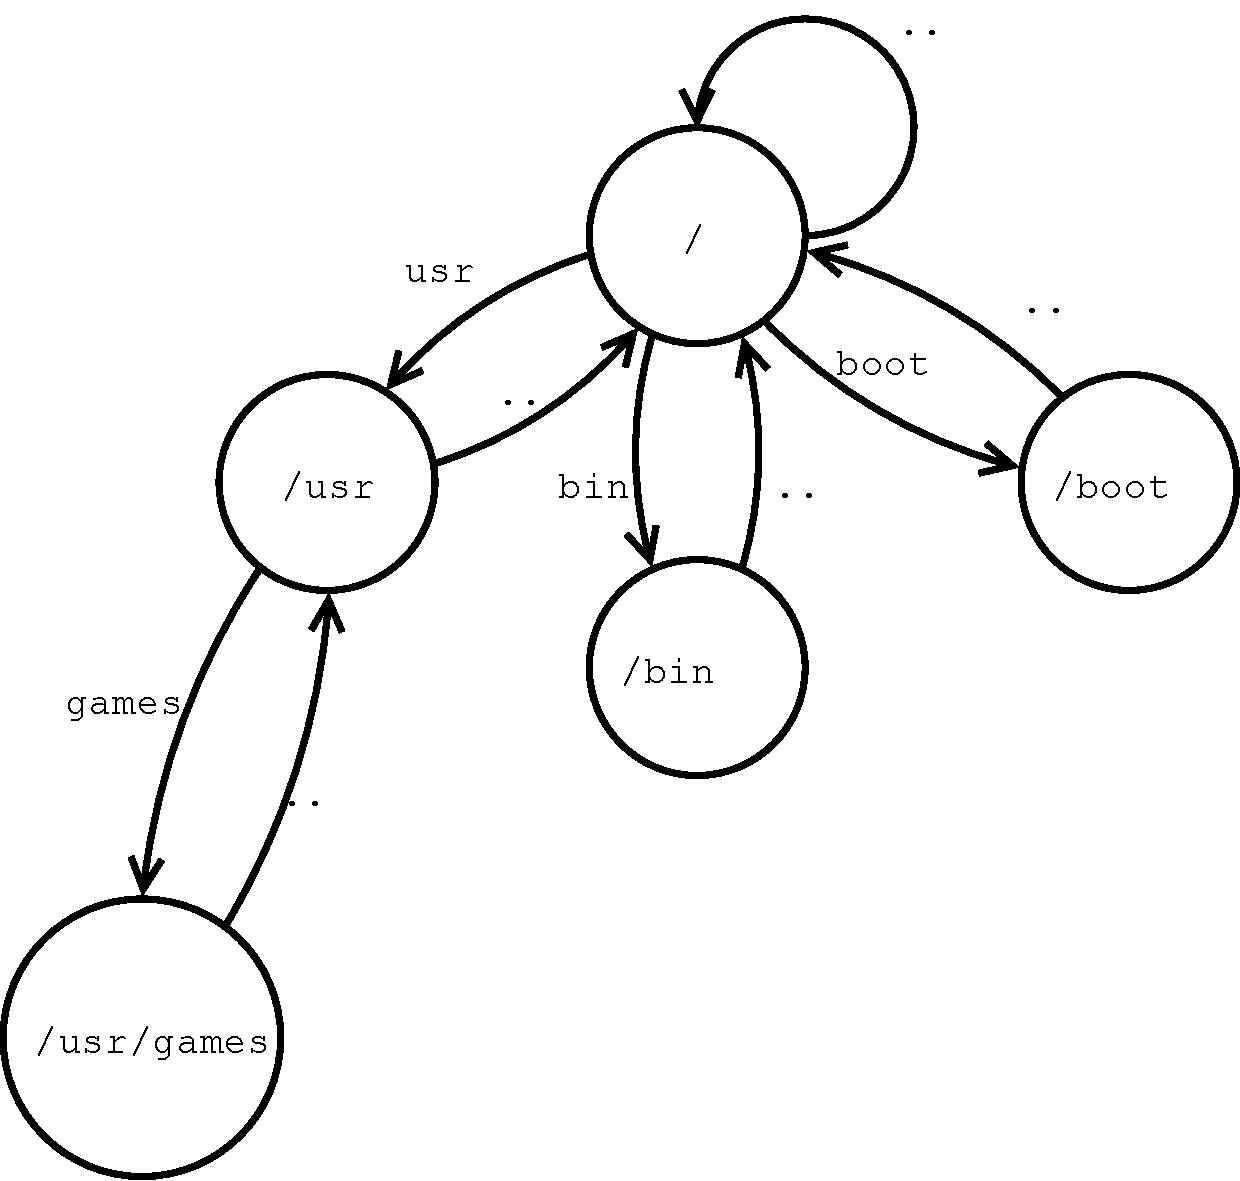
\includegraphics[width=\linewidth]{filesystems}
    \caption{Ejemplo de sistema de ficheros}
    \label{img:extensions}
\end{figure}

En esta figura, cada directorio tiene enlazados aquéllos dentro de él, y todos
ellos muestran a dónde enlaza el directorio \verb!..! que está dentro de ellos.
Como puedes ver, para llegar a una ruta como \verb!/usr/games! sólo tenemos
que ir dando <<saltos>> desde un directorio al siguiente. Si quisiéramos
volver hacia atrás, podemos usar los directorios ficticios que apuntan al padre
de cada uno. El caso del raíz es especial, porque su directorio padre es él
mismo. En Windows el sistema es igual, pero no existe una raíz, sino varias,
siendo éstas las unidades de disco. Por otro lado, no tenemos por qué hacer
\verb!cd! directorio a directorio, podemos introducir rutas completas. Una ruta,
si no lo has deducido ya, es simplemente la sucesión de directorios que llevan,
desde uno dado, a otro. Hay dos tipos de rutas:
\begin{enumerate}
\item Rutas absolutas: Empiezan por barra inclinada (\verb!/!) e indican una
ruta desde el directorio raíz hasta uno concreto, por ejemplo:
\verb!/home/john/music/Beethoven_symphony.mp4! sería una ruta absoluta.
\item Rutas relativas: Son aquéllas cuyo inicio no es la raíz, sino el
directorio de trabajo. Por ejemplo: \verb!music/Beethoven_symphony.mp4! es una
ruta relativa que sólo apuntará a un archivo que existe
si en el directorio de trabajo actual existe
un directorio llamado \verb!music! y, dentro de éste, un archivo llamado
\verb!Beethoven_symphony.mp4!.
\end{enumerate}

Eso que sale cada vez que pulsas enter se llama \textit{prompt}, y en general
te muestra tu nombre de usuario (en mi caso: <<usuario>>), la máquina donde
estás (en mi caso: <<DESKTOP-U8OA808>>) y después el directorio de trabajo, si
cabe. Yo voy a sustituir el \textit{prompt} por únicamente
el símbolo del dólar en
los ejemplos que te muestre, para que quepa el texto mejor.
La primera vez que abriste la terminal, ésta mostraba una virgulilla (\verb!~!)
porque ese es un alias de tu
directorio \textit{home}, que es una ruta de los sistemas Linux donde el usuario
almacena sus archivos personales. En general esa ruta está en
\verb!/home/<nombre de usuario>!.

Ahora vamos a aprender a ver lo que hay en un directorio, el comando que hace
eso se llama \verb!ls!, si lo tecleas y pulsas enter, verás que... que no sale
nada. Eso es porque no hemos creado ningún archivo ni directorio en nuestra
\emph{home}, el comando que crea archivos es \verb!touch!, escribe
\verb!touch prueba.txt! y pulsa enter, si haces \verb!ls!, verás que ahora
aparece.


\noindent
\begin{minipage}[H]{\linewidth}
\mbox{}
\begin{lstlisting}[style=terminalStyle]
\$ touch prueba.txt
\$ ls
prueba.txt
\$
\end{lstlisting}
\end{minipage}

\verb!ls! tiene muchas opciones, las opciones en comandos de Linux se ponen
con un guion delante, así que si te dicen que debes escribir, <<\verb!ls!
con las opciones a y l>>, debes escribir \verb!ls -l -a! o, juntando todas
las opciones en el mismo guion: \verb!ls -la!. Debería pasar algo como esto:

\noindent
\begin{minipage}[H]{\linewidth}
\mbox{}
\begin{lstlisting}[style=terminalStyle]
\$ ls -la
total 8
drwxr-xr-x 1 usuario usuario  512 Jul  8 19:05 .
drwxr-xr-x 1 root    root     512 Jul  7 22:37 ..
-rw-r--r-- 1 usuario usuario  220 Jul  7 22:37 .bash_logout
-rw-r--r-- 1 usuario usuario 3771 Jul  7 22:37 .bashrc
drwxr-xr-x 1 usuario usuario  512 Jul  7 22:37 .landscape
-rw-rw-rw- 1 usuario usuario    0 Jul  8 18:25 .motd_shown
-rw-r--r-- 1 usuario usuario  807 Jul  7 22:37 .profile
-rw-rw-rw- 1 usuario usuario    0 Jul  8 19:05 prueba.txt
\end{lstlisting}
\end{minipage}



Como verás, hay muchos archivos que tú no has creado. Esto es porque la opción
\verb!a! hace que \verb!ls! nos muestre \textbf{todos los archivos}, incluidos
los ocultos, que son los que empiezan por punto (\verb!.!). Y la opción \verb!l!
hace que salgan en una lista, y con información sobre ellos. Los directorios
ocultos empiezan con punto, y esto provoca que cuando haces un \verb!ls! normal
no aparezcan, convenientemente, los directorios punto y punto-punto.
Si esto te intimida, no te preocupes, es normal, y tengo buenas noticias, el WSL
ve los directorios que tienes en tu sistema Windows, así que puedes crear una
carpeta en tu escritorio y trabajar con el explorador de Windows, para crear
o eliminar los archivos.

\subsection{Instalar el compilador}
Ahora que ya has instalado una distribución de Linux que puedes usar, vamos
a instalar el compilador. Para ello ejecuta los comandos que salen a
continuación y, si te preguntan si quieres continuar, di que sí.

\noindent
\begin{minipage}[H]{\linewidth}
\mbox{}
\begin{lstlisting}[style=terminalStyle]
$ sudo apt update
#Aquí saldrá mucho texto, ignóralo.
$ sudo apt install build-essential
.......
After this operation, 189 MB of additional disk space will be used.
Do you want to continue? [Y/n] y
........
\end{lstlisting}
\end{minipage}



Ahora ya deberías tener instalado el compilador de C, que se llama GCC (por
sus siglas en inglés: \textit{GNU Compiler Collection}).
Para ver si es cierto, haz lo que sale a continuación.


\noindent
\begin{minipage}[H]{\linewidth}
\mbox{}
\begin{lstlisting}[style=terminalStyle]
\$ gcc -v
Using built-in specs.
COLLECT_GCC=gcc
COLLECT_LTO_WRAPPER=/usr/lib/gcc/x86_64-linux-gnu/9/lto-wrapper
OFFLOAD_TARGET_NAMES=nvptx-none:hsa
OFFLOAD_TARGET_DEFAULT=1
Target: x86_64-linux-gnu
Configured with: ../src/configure -v --with-pkgversion='Ubuntu 9.3.0-17ubuntu1~20.04' --with-bugurl=file:///usr/share/doc/gcc-9/README.Bugs --enable-languages=c,ada,c++,go,brig,d,fortran,objc,obj-c++,gm2 --prefix=/usr --with-gcc-major-version-only --program-suffix=-9 --program-prefix=x86_64-linux-gnu- --enable-shared --enable-linker-build-id --libexecdir=/usr/lib --without-included-gettext --enable-threads=posix --libdir=/usr/lib --enable-nls --enable-clocale=gnu --enable-libstdcxx-debug --enable-libstdcxx-time=yes --with-default-libstdcxx-abi=new --enable-gnu-unique-object --disable-vtable-verify --enable-plugin --enable-default-pie --with-system-zlib --with-target-system-zlib=auto --enable-objc-gc=auto --enable-multiarch --disable-werror --with-arch-32=i686 --with-abi=m64 --with-multilib-list=m32,m64,mx32 --enable-multilib --with-tune=generic --enable-offload-targets=nvptx-none=/build/gcc-9-HskZEa/gcc-9-9.3.0/debian/tmp-nvptx/usr,hsa --without-cuda-driver --enable-checking=release --build=x86_64-linux-gnu --host=x86_64-linux-gnu --target=x86_64-linux-gnu
Thread model: posix
gcc version 9.3.0 (Ubuntu 9.3.0-17ubuntu1~20.04)
\end{lstlisting}
\end{minipage}


Si te sale un texto parecido, enhorabuena, ya has instalado el compilador de C.
Ahora vamos, (por fin, estarás pensando) a empezar a aprender los conceptos del
lenguaje.


\section{Tu primer programa; ¡dile hola al mundo!}

Vamos a navegar a esa carpeta que tienes en tu escritorio, las unidades de tu
ordenador (los <<discos>> C, D, E...) se presentan en tu WSL en los
directorios dentro de
\verb!/mnt/!, así, \verb!C:! sería: \verb!/mnt/c!. A continuación te dejo el
ejemplo de cómo navegar en Linux a una carpeta llamada \verb!hola_mundo! en
tu escritorio de Windows. Puedes crearla ahora.


\noindent
\begin{minipage}[H]{\linewidth}
\mbox{}
\begin{lstlisting}[style=terminalStyle]
\$ cd /mnt/c/Users/Usuario/Desktop/
\$ cd hola_mundo
\$ pwd
/mnt/c/Users/Usuario/Desktop/hola_mundo
\$
\end{lstlisting}
\end{minipage}


Ahora que ya estás en la carpeta, ábrela en el explorador de Windows, porque
nos queda una última configuración, en la ventana del explorador de archivos,
arriba, pincha en la pestaña <<vista>> y marca la casilla donde pone
<<extensiones de nombre de archivo>>. Te dejo una foto de cómo debe quedar:

\begin{figure}[H]
    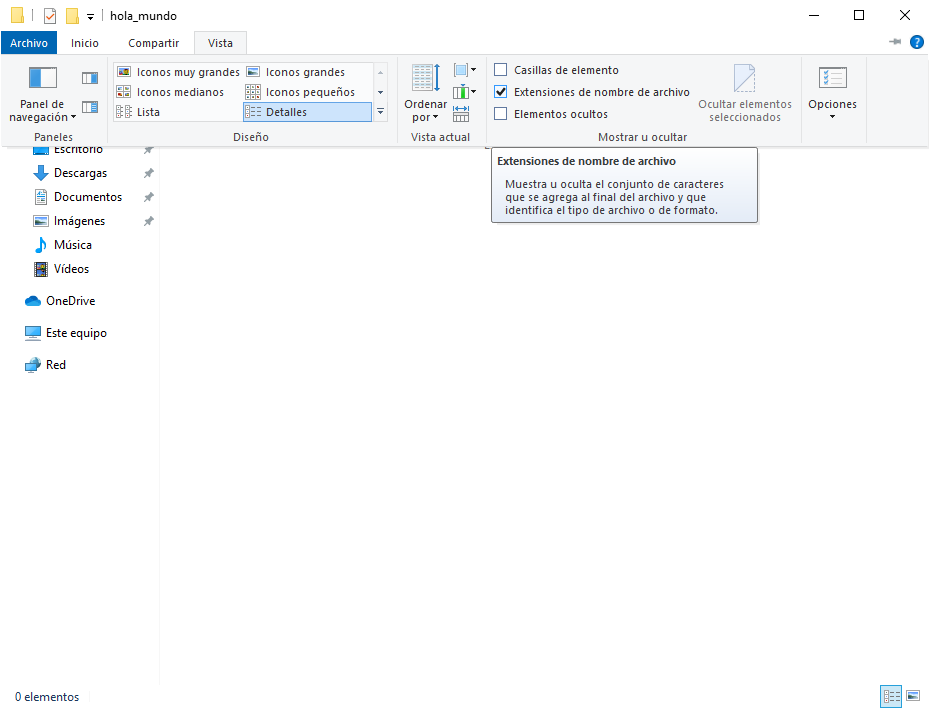
\includegraphics[width=\linewidth]{extensions}
    \caption{Configurar ver las extensiones}
    \label{img:extensions}
\end{figure}

Ahora, con el método que prefieras (la terminal o el ratón), crea en esa
carpeta un archivo llamado \verb!hola_mundo.c!. Y ábrelo con el bloc de notas
de Windows, y cuando digo el bloc de notas, no me refiero ni al wordPad ni a
Word, sino al bloc de notas. En ese documento vamos a escribir esto:

\begin{figure}[H]
\begin{verbatim}
#include <stdio.h>

int main(void)
{
        printf("¡Hola, mundo!\n");
}
\end{verbatim}
\end{figure}

Te aclaro que la línea que sale desplazada a la derecha es porque tiene
espacios delante, puedes poner dos, cuatro u ocho, yo recomiendo cuatro en
términos generales.
Después guárdalo, y acude a la terminal, deberías tener el fichero en el
directorio. Haz un \verb!ls! para comprobarlo. Te recuerdo que si has
cambiado de directorio de trabajo o has cerrado la terminal y vuelto a abrirla,
deberás volver a navegar a este directorio para poder ver sus archivos y
trabajar con él.
Ahora vamos a compilar nuestro
primer programa. Para eso, estando en el directorio que hemos creado
(\verb!hola_mundo!) invocaremos a gcc. Debería verse así:


\noindent
\begin{minipage}[H]{\linewidth}
\mbox{}
\begin{lstlisting}[style=terminalStyle]
\$ ls
hola_mundo.c
\$ gcc -o hola_mundo.elf hola_mundo.c
\end{lstlisting}
\end{minipage}


Al hacer esto, habrá aparecido un archivo llamado \verb!hola_mundo.elf! en la
carpeta. ¡Enhorabuena!, ese es tu primer programa en C. ¿Qué hace? Imprime
<<¡Hola, mundo!>>. Si haces doble clic en él verás que Windows no sabe abrirlo,
porque es un ejecutable para Linux, por ello, en la terminal, escribe
\verb!./hola_mundo.elf!. Si recuerdas lo que dije antes, una ruta que no empieza
en el directorio raíz (\verb!/!) es una ruta relativa, y el directorio punto
\textbf{es el directorio de trabajo}. Cuando a una terminal le indicas un
comando y pulsas enter, busca un programa con ese nombre en unos directorios
que vienen configurados en tu sistema operativo. Si quieres ejecutar cualquier
otro programa (u otras cosas que se pueden ejecutar, pero no vienen al caso
ahora) debes indicar una ruta, relativa o absoluta. Para que la terminal
sepa que estamos introduciendo una ruta y no un comando, la empezamos por
\verb!.!, es decir, este mismo directorio. Cuando escribas la orden y le des
a enter, debería verse lo siguiente:

\noindent
\begin{minipage}[H]{\linewidth}
\mbox{}
\begin{lstlisting}[style=terminalStyle]
\$ ./hola_mundo.elf
¡Hola, mundo!
\end{lstlisting}
\end{minipage}


Ahora que ya has compilado tu primer programa, quizás te hayas quedado un poco
frío, porque no entiendes qué hace, y es el momento en que yo adquiera un
compromiso contigo, el lector, y tú conmigo. Ese compromiso es que, por tu
parte, cuando no entiendas algo que aparece en los programas, confíes en que
en algún momento explicaré qué es. Por mi parte, mi compromiso es que procuraré
hacerlo lo antes posible.

De momento, te voy a explicar qué es el comando que hemos usado para compilar
nuestro programa: gcc es, como ya te dije, el compilador de C, la opción
\texttt{o} (recuerda que te expliqué lo que eran las opciones cuando te expliqué
cómo usar \verb!ls!) indica que lo que viene a continuación es el nombre del
programa que queremos crear y, finalmente, el nombre de nuestro fichero de
código fuente. Si detrás de la opción \verb!-o! escribieras otro nombre, el
programa resultante se llamaría así, de aquí en adelante la mayoría de los
ejemplos se compilarán como \verb!main.exe!.

\subsection{Editor de texto}
Tu primer programa lo has abierto con el Bloc de notas, pero editar código
fuente con eso es bastante insufrible. En parte porque como verás más adelante
lo normal es editar archivos de código fuente con un editor que coloree las
palabras más importantes (más adelante verás cuáles) y te ayude con cosas como
saber dónde terminan las llaves o paréntesis que has abierto. Si quieres
editar tu código, hay una gran variedad de editores para ello, aquí te dejo
una lista. En el manual no haré referencia a comandos específicos del editor.
Algunos editores que puedes usar son:
\begin{enumerate}
\item Visual Studio Code.
\item Atom.
\item Sublime Text.
\item Notepad++.
\end{enumerate}

\section{Primeros pasos}

Ahora que ya sabes lo que es un fichero de código fuente te voy a presentar
cómo vamos a incluir los fragmentos de código fuente en el manual.
Revisitemos el programa \verb!hola_mundo.c!.

\noindent
\begin{minipage}[H]{\linewidth}
\mbox{}
\begin{lstlisting}[style=C, caption={Hola Mundo en C},
label={lst:helloWorld}]
#include <stdio.h>
int main(void)
{
    printf("¡Hola, mundo!\n");
}
\end{lstlisting}
\end{minipage}

Como puedes ver, las líneas están numeradas, y hay palabras que salen en color
azul, y otras en rojo. Las palabras que salen en azul son las llamadas palabras
clave, (en inglés \textit{key words}), de momento, quédate con que todos tus
programas deben contener las líneas 1, 2, 3 y 5, y que entre la 3 y la 5
escribirás las instrucciones que compondrán tus archivos de código.
\subsection{Variables}
¡Por fin empieza lo bueno! Una de las primeras cosas que hacen falta en un
programa son \textbf{variables}, una variable simboliza un espacio en la
memoria del ordenador en que guardamos cosas. Cuando creamos una variable, le
decimos al ordenador <<reserva espacio en tu memoria para guardar un dato>>.
C es un lenguaje de los que se llaman tipados, es decir, que cada variable
tiene un tipo, y éste no puede cambiar una vez que esa variable se crea. En C
hay una serie de tipos básicos que te presento en una práctica tabla.


\begin{table}[H]
    \centering
    \begin{tabularx}{\linewidth}{|c|c|c|Y|}
        \hline
        \textbf{Nombre} &\textbf{Tamaño} (en bytes)&\textbf{Rango}&\textbf{Uso} \\\hline
        \texttt{char} & 1 & $[-128, 127]\vphantom{\matrix{1\cr1\cr1\cr}}$ & Un carácter de texto o un byte\\\hline
        \texttt{short}& 2 & $[-32\,768, 32\,767]\vphantom{\matrix{1\cr1\cr1\cr}}$& Números en ese rango (generalmente puertos de red)\\\hline
        \texttt{int}&   4  & $[-2\,147\,483\,648, 2\,147\,483\,647]\vphantom{\matrix{1\cr1\cr1\cr}}$&Tipo general para números enteros\\\hline
        \texttt{float}& 4 & $[\pm3.4\cdot{}10^{-38}, \pm3.4\cdot{}10^{38}]\vphantom{\matrix{1\cr1\cr1\cr}}$ & Números decimales de precisión simple\\\hline
        \texttt{double}&8 &$[\pm1.79\cdot{}10^{-308}, \pm1.79\cdot{}10^{308}] \vphantom{\matrix{1\cr1\cr1\cr}}$ & Números decimales de precisión doble\\\hline
    \end{tabularx}
    \caption{Tipos básicos de C}
    \label{tab:basicTypes}
\end{table}

Una tabla así puede ser abrumadora, pero es sencillo. Cuando declaramos
(creamos) una variable, debemos decir de qué tipo es. Me gusta decir que las
variables son como cajas y que, según su tipo, en esa caja entran unas cosas
u otras. Para declarar una variable, debes poner su tipo, y un nombre, ¡y no
olvides terminar la línea en punto y coma (;)! Además de declararlas, debemos
aprender a darles un valor. Eso se llama <<asignar un valor>> y se hace con el
símbolo de igual (\verb!=!). Para darle un valor se pone el nombre de la
variable, el símbolo de igual y el valor, veamos unos ejemplos, y te explico
algunas salvedades.

A propósito del nombre: el nombre
de una variable se compone de letras, números y guiones bajos.
El nombre de una variable no debería estar escrita en mayúsculas, pero puede
contenerlas.
No puede empezar por número y \textbf{no deberías empezarla por un guion bajo}.
En general, puedes usar dos notaciones para escribir nombres en C
(y en cualquier lenguaje de programación):
\begin{enumerate}
\item \emph{Camel Case}: Si un nombre contiene varias palabras, se deben
escribir juntas, con la primera palabra de cada una en mayúscula. Por ejemplo:
\verb!betterValue! o \verb!targetNumber!. Se llama así porque esas mayúsculas
recuerdan a las jorobas de un camello.
\item \emph{Snake Case}: Las palabras aparecen separadas por guiones bajos,
en minúscula totalmente, por ejemplo: \verb!better_value! o
\verb!target_number!. Se llama así porque la forma de los nombres escritos en
este modo recuerda a una serpiente que ha comido animales y tiene bultos en su
cuerpo.
\end{enumerate}

\noindent
\begin{minipage}[H]{\linewidth}
\mbox{}
\begin{lstlisting}[style=C, caption={Creación y asignación de variables},
label={lst:variableAsignation}]
#include <stdio.h>
int main(void)
{
    char letter = 'a';
    char byte = 120;
    short shorty = 5520;
    int money_i_want;
    float money_i_have = 3.22F;
    double money_you_have = 52.55;

    money_i_want = 450000;
    shorty = 11111;
}
\end{lstlisting}
\end{minipage}

Los ordenadores no entienden de letras, sólo de números, así que, en el fondo,
cuando le dices que \verb!letter! es igual a \verb!'a'!, le dices que es igual
al número que significa esa letra. Nota que para poner el valor de un
\texttt{char} debes usar comillas simples, en el teclado español, es lo que
sale al pulsar la tecla de la interrogación de cierre.
La correspondencia entre letras y números está escrita en la tabla ASCII, si
quieres leerla, te dejo un \href{https://elcodigoascii.com.ar/}{enlace}
a un sitio donde la puedes consultar.
Si miras allí, verás que la letra a es el valor
97. Después asignamos a otro \verb!char!
un valor numérico, en la línea 7 puedes ver que declaramos una variable sin
darle un valor. Esto es perfectamente correcto, pero, ¡cuidado!,
\textbf{una variable a la que no le das valor tiene un valor aleatorio}.
Darle valor a una variable por primera vez se llama <<inicializarla>>.
Por este motivo muchos profesores te dirán que siempre que declares
una variable le des un valor inmediatamente.

En las líneas 11 y 12 le damos
valor a variables que hemos declarado anteriormente, y quiero detenerme en el
caso de la línea 12. Al principio puede parece que al escribir
\verb!shorty = 5520;! estamos enunciando una igualdad matemática, es decir,
que eso siempre será así, pero en C no trabajamos con <<leyes>>, sino con
instrucciones, así que no debes leer esa línea como <<\verb!shorty! es igual a
5520>> sino como <<He asignado a \verb!shorty! el valor 5520>>. Es decir, has
metido en esa <<caja>> un 5520, pero nada te impide sacar ese valor y meter
otro número como estamos haciendo.

Los valores que escribe el programador en el código se llaman <<literales>>.
Creo que el nombre no necesita explicación. Cada literal tiene un tipo
determinado, al igual que las variables. Más adelante veremos por qué eso es
importante. De momento, recuerda que se llama literal a los valores que el
programador escribe en el código explícitamente. Por ejemplo, los números
(como 5520) o las letras (\verb!'a'!)
Además de literales, podemos asignarle a una
variable el valor de una \textbf{expresión}, una expresión es cualquier
texto escrito en lenguaje C que tenga un valor. De momento, nos vamos a limitar
a asignar unas variables a otras. Por ejemplo:

\noindent
\begin{minipage}[H]{\linewidth}
\mbox{}
\begin{lstlisting}[style=C, caption={Asignación de variables entre ellas},
label={lst:variableAsignationBetween}]
#include <stdio.h>
int main(void)
{
    int a = 3;
    int b = 2;

    a = b;
}
\end{lstlisting}
\end{minipage}

En la línea 7 podemos ver como asigno a la variable \verb!a! el valor de
\verb!b!, es decir, ahora \verb!a! valdrá 2. Como ver esto así es difícil, voy a
incluir en el siguiente
ejemplo una serie de líneas que contienen la palabra \verb!printf!, te sonará
porque la usamos en nuestro primer ejemplo, sirve para que el programa escriba
cosas en tu terminal. Después te enseñaré a usarla.
De momento, simplemente copia el
siguiente programa en tu archivo de código fuente y compila como lo hicimos
antes. (Copiar desde un PDF suele ser mala idea, teclea a mano, así practicarás)

\noindent
\begin{minipage}[H]{\linewidth}
\mbox{}
\begin{lstlisting}[style=C, caption={Ejemplo final de variables},
label={lst:variableFinalExample}]
#include <stdio.h>
int main(void)
{
    int a = 3;
    int b = 10;
    printf("a vale: %d\n", a);
    a = b;
    printf("b vale: %d y a vale lo mismo, es decir: %d\n", b, a);
    b = 22;
    printf("b vale: %d, a sigue valiendo %d\n", b, a);
}
\end{lstlisting}
\end{minipage}


Si tecleas este programa, lo compilas y lo ejecutas
debería salirte algo como esto:


\noindent
\begin{minipage}[H]{\linewidth}
\mbox{}
\begin{lstlisting}[style=terminalStyle]
\$ ./main.elf
a vale: 3
b vale: 10 y a vale lo mismo, es decir: 10
b vale: 22, a sigue valiendo 10
\end{lstlisting}
\end{minipage}

Como puedes ver, cuando se escribe \verb!a = b!,
\textbf{los valores de \texttt{a} y \texttt{b} no quedan ligados}. Pero al
asignar cualquier valor (tanto literal como de una expresión) a una variable
hay que tener cuidado. Volviendo a la metáfora de las cajas, en una caja caben
objetos de determinadas formas y tamaños, si un dato es,
por ejemplo, un número decimal (ya sea éste \textit{float} o \textit{double})
al ser asignado a una variable entera, perderá su parte decimal. Pero hay más,
si aplicas la lógica, ¿qué pasaría si asignas un número como 1203 a un
\texttt{char}? Si acudes a la tabla \ref{tab:basicTypes}:
\nameref{tab:basicTypes}, verás que 1203 está fuera del rango del
char. Bien, lo que pasa es que no sabes lo que pasa. La manera elegante de decir
esto es: <<comportamiento no definido>> o <<\textit{undefined behaviour}>>.
El siguiente programa es un ejemplo de esto:


\noindent
\begin{minipage}[H]{\linewidth}
\mbox{}
\begin{lstlisting}[style=C, caption={Asignaciones inválidas},
label={lst:invalidAssignations}]
#include <stdio.h>
int main(void)
{
    char c = 1500;
    short s = 5555555;
    float f = 3.8e105;

    printf("c: %d\n", c);
    printf("s: %hd\n", s);
    printf("f: %f\n", f);
}
\end{lstlisting}
\end{minipage}


Si lo compilas, el compilador te dará una serie de mensajes llamados
\textit{warnings}. Advertencias de que algo que has escrito, si bien es
<<correcto>>, no tiene pinta de <<estar bien>>. Si por ejemplo escribieras
en español: <<¡Mas me duele a mí!>>, aunque es una frase correcta, es probable
que quisieras escribir <<¡Más me duele a mí!>>, y no significan lo mismo. Si
compilamos y ejecutamos, en la terminal debería aparecer algo así:


\noindent
\begin{minipage}[H]{\linewidth}
\mbox{}
\begin{lstlisting}[style=terminalStyle]
\$ gcc -o main.exe main.c
main.c: In function 'main':
main.c:86:14: warning: overflow in conversion from 'int' to 'char' changes value from '1500' to '-36' [-Woverflow]
   86 |     char c = 1500;
      |              ^~~~
main.c:87:15: warning: overflow in conversion from 'int' to 'short int' changes value from '5555555' to '-15005' [-Woverflow]
   87 |     short s = 5555555;
      |               ^~~~~~~
\$ ./main.exe
c: -36
s: -15005
f: inf
\end{lstlisting}
\end{minipage}


Como puedes ver, ni el \texttt{char} vale 1.500 (porque no puede), ni el
\texttt{short} vale 5.555.555, porque tampoco puede. Pero el compilador no dice
nada sobre el \texttt{float}, al que le hemos asignado un literal fuera de
rango. El motivo es que los \texttt{float} y \texttt{double} en C tienen un
valor especial llamado \textit{infinity}, que simboliza el infinito. Esto es
porque, como veremos a continuación, no representan los números de manera
totalmente correcta, y por eso pueden valer más y menos infinito.

Detengámonos en el problema de los números decimales. Si sabes cómo funciona
el código binario, sabrás que en un número binario de $n$ bit se pueden
representar $2^n$ valores. En el caso de los números decimales, usamos un
sistema complejo denominado IEEE 754. No voy a entrar en detalles, pero el
principal problema de esta manera de representar los números decimales es que
no sólo no es exacta (por ejemplo, el número 0,1 no se puede representar
exactamente) sino que además su precisión \textbf{varía} según el rango en que
esté el número representado. ¿Qué quiere decir esto? Que si cerca del cero los
\textit{float} pueden distinguir entre 1,10 y 1,11, a lo mejor no pueden
distinguir entre 1000000,10 y 1000000,11. Ten esto en cuenta si haces
programas que utilicen números decimales.

Como has visto aquí, hay asignaciones permitidas y prohibidas entre
tipos, las permitidas (las que el compilador no ve como algo malo), se llaman
conversiones implícitas, su nombre viene de que tú no tienes que hacer nada
para que ocurran, por ejemplo, como hemos visto, asignando un \verb!char!
a un entero. Posteriormente te enseñaré a hacer conversiones entre tipos
explícitamente.

\subsection{Imprimir cosas}
Entre programadores se llama imprimir a escribir cosas en ficheros y,
especialmente, por pantalla, como tu primer programa que escribía en pantalla
<<¡Hola, mundo!>>. No quiero adelantar más de lo necesario, porque detrás de
lo que usamos para imprimir por pantalla hay varios conceptos, pero necesito que
sepas imprimir cosas para que puedar probar tus propios programas.

Para imprimir algo en pantalla debes usar la palabra \texttt{printf}. Con una
sintaxis que es un poco complicada. Debes poner \texttt{printf}, un paréntesis y
una cosa llamada <<formato>>. El formato es el texto que se va a imprimir,
rodeado de comillas dobles (\texttt{"}). Para incluir variables en esa
impresión, debes poner los llamados <<especificadores>>, que son textos
especiales que indican \textbf{el tipo} de las variables que quieres imprimir.
Después del formato, pondremos las variables que vayamos a imprimir, separadas
por comas, en el orden en que pusimos sus especificadores. Además, hay ciertos
caracteres que se deben poner de manera especial, los saltos de línea y
los tabuladores. Esto es un poco confuso, así que te dejo dos tablas donde
puedes ver los especificadores y los caracteres especiales.

\begin{table}[H]
\centering
\begin{tabularx}{\linewidth}{|c|Y|}
\hline
\textbf{Especificador} & \textbf{Tipo que imprime}                       \\ \hline
\texttt{\%d}& Enteros (\texttt{int})                                     \\ \hline
\texttt{\%f}& \texttt{float}      \\ \hline
\texttt{\%lf}& \texttt{double}      \\ \hline
\texttt{\%hd}& \texttt{short}                                            \\ \hline
\texttt{\%c}& \texttt{char} como letras (no números)                     \\ \hline
\texttt{\%s}& Texto, escrito como \texttt{\textquotedbl Un texto\textquotedbl}, comillas incluidas. \\ \hline
\texttt{\%p}& Punteros, son una cosa avanzada y la explicaré varias secciones más adelante \\ \hline
\end{tabularx}
\caption{Especificadores de formato en C}
\label{tab:formatSpecifierC}
\end{table}

Por otro lado, los caracteres especiales son éstos, y se ponen con una barra
inclinada invertida (\textbackslash{}) delante. En la tabla incluyo ya la barra
inclinada invertida correspondiente. Además, como los especificadores empiezan
con el símbolo de porcentaje, si quieres imprimir uno, debes ponerlo dos veces.

\begin{table}[H]
\centering
\begin{tabularx}{\linewidth}{|c|Y|}
\hline
\textbf{Secuencia} & \textbf{Carácter impreso} \\\hline
\texttt{\textbackslash{}\textbackslash{}} & Barra inclinada inversa            \\\hline
\texttt{\textbackslash{}n}& Nueva línea                         \\\hline
\texttt{\textbackslash{}t}& Tabulador (imprime espacios hasta que se alinea a una columna de 4 espacios)   \\\hline
\texttt{\%\%}& Imprime sólo un símbolo de porcentaje   \\\hline
\end{tabularx}
\caption{Imprimir caracteres especiales en C}
\label{tab:specialCharsC}
\end{table}

Esto es muy pedregoso, así que vamos a ver un ejemplo.



\noindent
\begin{minipage}[H]{\linewidth}
\mbox{}
\begin{lstlisting}[style=C, caption={Ejemplo de impresión.},
label={lst:decimalvsintergerDivision}]
#include <stdio.h>
int main(void)
{
    int entero = 654654;
    short shorty = 25254;
    char charty = 'a';
    double decimal = 2.3;
    printf("El entero vale:\t%d\nEl short vale:\t%hd\nEl char es la letra:\t%c\nEl decimal vale:\t%f\n", entero, shorty, charty, decimal);
}
\end{lstlisting}
\end{minipage}


La línea es muy larga y en esta página se escribe como varias, pero tú deberías
escribirlo todo como una sola línea. (Si te fijas, sólo hay un número, eso
indica que es la misma línea pero partida para que quepa) El programa, una vez
compilado, debería arrojar este resultado:



\noindent
\begin{minipage}[H]{\linewidth}
\mbox{}
\begin{lstlisting}[style=terminalStyle]
\$ ./main.exe
El entero vale: 654654
El short vale:  25254
El char es la letra:    a
El decimal vale:        2.300000
\end{lstlisting}
\end{minipage}


Corolario final: \texttt{printf} no añade nada que tú no le pongas, incluidos
saltos de línea, así que si quieres imprimir lo siguiente en una línea distinta,
acuérdate de poner \verb!\n! al final del formato. Además, siempre es
recomendable que lo último que imprima tu programa sea un salto de línea, si no,
podría dejarse cosas sin imprimir, porque la terminal se fuerza a imprimir las
cosas cuando recibe una línea nueva.

\subsection{Operadores}
Jugar a los trileros con los valores de las variables que declaras en
tu programa es... aburrido, lo sé, por ello, vamos a aprender a hacer
operaciones con ellas.
En C (y en cualquier lenguaje de programación) existen los llamados
\textbf{operadores}. Son símbolos que nos permiten realizar un cálculo.
Los operadores son un concepto matemático, y se aplican a una
serie de argumentos, o, mejor dicho, operandos. En
matemáticas, los símbolos $+$, $-$, $\times$, y $/$ son
operadores para la suma, la resta, la multiplicación y la división,
respectivamente.
Del mismo modo que hemos hecho con los tipos básicos, te los
voy a presentar en una tabla y después veremos ejemplos de cómo se usan.

\begin{table}[H]
\centering
\begin{tabularx}{\linewidth}{|c|Y|}
\hline
\bf Operador & \bf Descripción \\ \hline
\tt + & Suma. Suma tanto números enteros como decimales y entre ellos. \\\hline
\tt - & Resta. Sustrae del operando de a su izquierda el valor del operando a su derecha. \\\hline
\tt / & División. Devuelve el resultado de la división del operando izquierdo entre el derecho. Nótese que, \textbf{si ambos operandos son enteros}, el operador realiza la división entera, es decir, \textbf{sin decimales}. \\\hline
\tt * & Multiplicación. El asterisco hace muchas cosas en C, pero de momento esta la primera de sus funciones que descubrirás. El resultado de una multiplicación es un \textbf{double}.\\\hline
\tt ++ & Incremento. Hace que un número (decimal o no) aumente en una unidad. Puede ser prefijo (delante del número) o postfijo (detrás del número). \\\hline
\tt -{}- & Decremento. Funciona como el incremento, pero disminuye el número en una unidad. \\\hline
\tt \% & Módulo. Es un operador que devuelve el resto (o residuo) de la división entera entre el operando izquierdo y el derecho. \\\hline
\end{tabularx}
\caption{Operadores matemáticos básicos}
\label{tab:mathOperators}
\end{table}

En la sección anterior te dije que a una variable le podíamos asignar un valor.
También dije que una expresión es un fragmento de código C con un valor, y que
el nombre de una variable, sola, es una expresión. Ahora que tenemos operadores
podemos realizar expresiones más complejas, por ejemplo, \verb!a+b! sería una
expresión cuyo valor sería la suma de \verb!a! y \verb!b!. ¡Ya podemos hacer
cálculos!

Hay que tener cuidado, porque, como ya te dije, toda expresión en C tiene
\textbf{un tipo}, y, como vimos en la sección anterior, asignar un valor de
un tipo incorrecto a una variable resulta en errores. Por ejemplo, el operador
de la división se comporta distintamente si sus operandos (los números
divididos) son enteros o decimales. Veamos un ejemplo:


\noindent
\begin{minipage}[H]{\linewidth}
\mbox{}
\begin{lstlisting}[style=C, caption={División entera contra división
decimal},
label={lst:decimalvsintergerDivision}]
#include <stdio.h>
int main(void)
{
    double d1 = 1/3;
    printf("d1: %f\n", d1);

    double d2 = 1.0/3;
    printf("d2: %f\n", d2);
}
\end{lstlisting}
\end{minipage}


Si compilas y ejecutas el programa verás que sale este resultado:


\noindent
\begin{minipage}[H]{\linewidth}
\mbox{}
\begin{lstlisting}[style=terminalStyle]
\$ ./main.exe
d1: 0.000000
d2: 0.333333
\end{lstlisting}
\end{minipage}



Lo que parecen operaciones iguales, dan resultados distintos, y esto es porque
el \textbf{tipo} de los operandos es distinto. En C, un valor literal entero
es un \verb!int!, y el operador división, cuando opera dos enteros, tiene tipo
entero. Sin embargo, cuando \textbf{cualquiera de los dos} operadores es
decimal, realiza la operación decimal, y su tipo es \verb!double!.

Los operadores \verb!++! y \verb!--! son especiales, porque son operadores
unarios. Un operador unario es aquél que sólo se aplica a un operando. Por
ejemplo, en matemáticas existe el operador raíz cuadrada, denotado por el
símbolo $\sqrt{\phantom{2}}$ que, aplicado a un único número, nos da
el número (o números) que elevado al cuadrado nos dan el operando.
Los operadores incremento y decremento son unarios, y, además, se
pueden escribir delante o detrás de su operando. Estos operadores son
especiales porque no sólo dan un valor, sino que \textbf{cambian el valor
del operando al que se aplican}. Simplemente: si \verb!a! vale tres y realizamos
\verb!a++!, \verb!a! pasará a valer cuatro, pero si asignamos el valor de la
operación a otra variable, esa variable tendrá un valor determinado.
Veámoslo en código.


\noindent
\begin{minipage}[H]{\linewidth}
\mbox{}
\begin{lstlisting}[style=C, caption={Operadores de incremento y decremento},
label={lst:prefixAndPostfixOperators}]
#include <stdio.h>
int main(void)
{
    int a = 3;
    int b = ++a;
    printf("a: %d; b: %d\n", a, b);
    a = 3;
    int c = a++;
    printf("a: %d; c: %d\n", a, c);
}
\end{lstlisting}
\end{minipage}


Si lo ejecutas saldrá lo siguiente:


\noindent
\begin{minipage}[H]{\linewidth}
\mbox{}
\begin{lstlisting}[style=terminalStyle]
\$ ./main.exe
a: 4; b: 4
a: 4; c: 3
\end{lstlisting}
\end{minipage}


Quiero que entiendas bien lo que ocurre aquí: siempre que apliquemos el
operador incremento a una variable, ésta aumentará de valor en una unidad.
No obstante;
dependiendo de si lo hacemos prefijo o postfijo, el valor \textbf{de la
expresión} cambia. En el caso del operador prefijo, el valor de la expresión es
el valor de la variable \textbf{con el incremento aplicado} y si lo hacemos
postfijo, ese valor es el de la variable \textbf{antes de aplicar el operador}.
Te preguntarás qué necesidad hay de que haya un operador para esto. Bueno,
existe porque contar, tanto hacia delante como hacia atrás, es una operación
muy común. Así que para ahorrarnos líneas, en vez de escribir
\lstinline[style=C]!int b = a; a = a + 1;! podemos escribirlo como ya has
visto.

Siguiendo la línea de los operadores incremento y decremento, también hay
operadores que aúnan la asignación con alguna operación matemática, es decir,
sustituir \lstinline[style=C]!a = a * 3;! por
\lstinline[style=C]!a *= 3;!. Existen los mismos operadores para suma, resta,
división y módulo.

Finalmente, decirte que la \textbf{prioridad} de las operaciones es la misma
que en matemáticas: primero se ejecutan divisiones y multiplicaciones, después
restas y sumas. Las operaciones con la misma prioridad se ejecutan de izquierda
a derecha. El módulo está al mismo nivel que la multiplicación, y los operadores
de incremento y decremento siempre van los primeros. De todos modos, si tienes
dudas, pon paréntesis en lo que quieras que se ejecute primero.

\subsubsection{Cásting: conversiones explícitas}
Es normal que necesites que un tipo se convierta en otro, por ejemplo, en el
caso anterior, si los divisores fueran enteros,
tendrías que <<forzar>> a que uno fuera decimal para conseguir la división decimal.
También suele pasar que una variable que es un entero
deba ser <<metida>> en un \verb!char! porque sabes que es del rango correcto.
Para esto existe la herramienta del \textit{casting}, que en inglés es
<<moldear>> como quien vierte metal líquido en un molde. Con él, podemos
transformar un tipo en otro. Pero no es la panacea, las leyes de la lógica se
siguen aplicando, un \verb"char" no puede valer más de 127, aunque hagas
cástings. Veamos un ejemplo:



\noindent
\begin{minipage}[H]{\linewidth}
\mbox{}
\begin{lstlisting}[style=C, caption={Ejemplo de cásting},
label={lst:castingExample}]
#include <stdio.h>
int main(void)
{
    int a = 3;
    int b = 2;
    double result = (double)a / b;
}
\end{lstlisting}
\end{minipage}



En la línea 6 necesitamos que al menos unos de los operadores sea decimal
(ya sea \texttt{float} o \texttt{double}). Así que realizamos el cásting
a ese tipo del primer operando. La sintaxis del cásting es sencilla, pero
voy a explicarla detenidamente: debes poner el nombre del tipo al que quieres
hacer cásting entre paréntesis, y justo a su lado la expresión a la que quieres
hacérselo. Te dejo algunos ejemplos:
\begin{enumerate}
\item \lstinline[style=C]!(int) (decimal_number / other_decimal)!: Aquí
estamos haciendo cásting a entero del resultado de una división, como puedes
ver, necesitamos encerrar en paréntesis la división para que el cásting se haga
a esa expresión y no sólo al primer elemento.
\item \lstinline[style=C]!(char) (number % 128)! aquí estamos viendo uno
de los casos en que hacer cásting a un tipo más pequeño es bueno, si
\texttt{number} es un entero, al hacerle cásting a \verb!char!
podría haber problemas,
pero como hemos hecho módulo a 128, el resultado de la expresión siempre será
un número entre 0 y 127, que entra en el rango del \texttt{char}.
\end{enumerate}
A continuación te dejo una tabla de
conversiones válidas entre tipos básicos:

\begin{table}[H]
\begin{tabularx}{\linewidth}{|c|c|Y|Y|Y|Y|Y|}
\cline{3-7}
\multicolumn{2}{c|}{}&\multicolumn{5}{c|}{\textbf{Tipo de destino}}\\\cline{3-7}
\multicolumn{2}{c|}{}& \texttt{char}&\texttt{short}&\texttt{int}&\texttt{float}&\texttt{double} \\\cline{1-7}
\multirow{5}{*}[-5em]{\begin{sideways}\textbf{Tipo de origen}\end{sideways}}&\texttt{char} &OK&OK &OK &OK &OK \\\cline{2-7}
&\texttt{short} &Cásting (desbordamiento)&OK&OK&OK&OK \\\cline{2-7}
&\texttt{int} &Cásting (desbordamiento) &Cásting (desbordamiento)& OK&OK (precisión) & OK (precisión)\\\cline{2-7}
&\texttt{float} &Cásting (redondeo, desbordamiento)& Cásting (redondeo, desbordamiento)& Cásting (redondeo, desbordamiento)& OK& OK \\\cline{2-7}
&\texttt{double} &Cásting (redondeo, desbordamiento)& Cásting (redondeo, desbordamiento)& Cásting (redondeo, desbordamiento)& Cásting (redondeo, desbordamiento)&OK \\\cline{1-7}
\end{tabularx}
\caption{Conversiones de tipos en C}
\label{tab:conversions}
\end{table}

Donde pongo <<OK>> quiero decir que se produce una conversión implícita, pero
hay que tener cuidado. El rango del entero es muy grande, y puede ocurrir que
la precisión de un \texttt{float} o un \texttt{double} no llegue a la unidad
en los extremos del rango del entero. Te seré sincero, en el rango de los miles
de millones al que llega el entero, el \verb!float! (y más el \verb!double!)
es perfectamente capaz de
contener valores enteros con precisión, pero lo incluyo para que no se te
olvide el problema de la precisión. Donde pongo cásting e indico que puede
haber desbordamiento es porque estás convirtiendo un tipo más grande (en bytes)
a otro más pequeño, quien debe controlar si eso está bien hecho es el
programador, es decir, tú.

\subsubsection{Ejemplo final de programa con operadores}
Habiendo visto todo esto, podemos hacer nuestro primer programa que haga
<<algo>>, voy a darte como ejemplo un programa que calcula la
solución a un sistema de ecuaciones lineales, es decir:

$$
\left\{\matrix{ax+by = c \cr
               dx+ey = f}
\right.
$$

Con un sistema así, podemos aplicar el método de sustitución:

$$
(1)\; ax+by=c \to x= \frac{c-by}{a}
$$
$$
(2)\; dx+ey=f \to x=\frac{f-ey}{d}
$$
$$
(1) \;\mathrm{y} \; (2) \to \frac{c-by}{a} = \frac{f-ey}{d} \to
y=\frac{af-dc}{ae-db} \to x=\frac{f-e\cdot\frac{af-dc}{ae-db}}{d}
$$


\noindent
\begin{minipage}[H]{\linewidth}
\mbox{}
\begin{lstlisting}[style=C, caption={Cálculo de ecuación lineal},
label={lst:linealEquation}]
#include <stdio.h>
int main(void)
{
    int a = 1;
    int b = 3;
    int c = 8;
    int d = 2;
    int e = 7;
    int f = 12;

    double y = (a * f - d * c) / (a * e - d * b);
    double x = (f - e * y) / (d);

    printf("%dx+%dy=%d\n", a, b, c);
    printf("%dx+%dy=%d\n", d, e, f);
    printf("x = %f; y = %f\n", x, y);
}
\end{lstlisting}
\end{minipage}


Si copias este
programa, verás aplicado lo que he explicado sobre variables y expresiones.
Además, el programa cuenta con un problema, sólo resuelve \textbf{una} ecuación,
para que resuelva otra, o para cambiar algunos de los valores,
debemos cambiar el
programa y recompilarlo. Eso no es práctico, y los programas de verdad no
funcionan así. De momento la mayoría de nuestros programas serán así, porque
quiero enseñarte primero otras cosas más fundamentales. Hasta ahora, los
programas que hemos escrito se comportan de manera muy \textit{aburrida}, sólo
ejecutan una serie de instrucciones una detrás de otra. Pero en la vida real
los programas ejecutan instrucciones dependiendo de condiciones, o las ejecutan
varias veces, etc.

Otro de los problemas es que no podemos cambiar el comportamiento del programa
en determinadas condiciones. Si cambias el valor de los números en el
programa de ejemplo para que éste sea irresoluble, el programa fallará.
Haz la prueba, cambia los valores de \texttt{a}, \texttt{b}
y \texttt{c} a 1 y los de \texttt{d}, \texttt{e} y \texttt{f} a 2. Este
sistema tiene infinitas soluciones y hará que el programa falle. Si lo compilas
y lo ejecutas con los nuevos valores debería salir algo como esto:



\noindent
\begin{minipage}[H]{\linewidth}
\mbox{}
\begin{lstlisting}[style=terminalStyle]
\$ ./main.exe
1x+1y=1
2x+2y=2
x = -nan; y = -nan
\end{lstlisting}
\end{minipage}


¿Qué rayos es nan? Es uno de los valores especiales de los números decimales en
C (recuerda la IEEE 754), significa \textit{Not a Number}. Es decir, que el
resultado de esa operación que hemos hecho no es un número. ¿Por qué? Porque
hemos dividido entre cero. Y si sabes un poco de cálculo, sabrás que un número
dividido entre cero es una indeterminación, es decir, no sabemos qué es. Así lo
expresa C. Y tenemos suerte, si en vez de división flotante fuera división
entera, el programa se vería obligado a cerrar inesperadamente. Sería
interesante poder comprobar primero si el sistema tiene solución y después
calcularla. Eso se hace con estructuras de control, que es el siguiente
capítulo.

\section{Alterando el flujo normal del programa}
Como he introducido en la sección anterior, es conveniente poder hacer que el
programa haga una cosa u otra según una condición. Además, es posible (de hecho
es imprescindible) que el programa repita instrucciones basándose en
condiciones. Esto se llama alterar el flujo del programa, porque en vez de
ejecutar una línea después de la anterior, el ordenador podrá saltar de
un sitio a otro del programa, tanto hacia delante como hacia atrás.

\subsection{Sentencias condicionales}
Las sentencias condicionales son las que nos permiten hacer \textbf{diverger} el
flujo del programa dependiendo de una condición. Lo vas a entender
perfectamente con un diagrama que incluiré a continuación:
\begin{figure}[H]

% generated by Plantuml 1.2022.7
\definecolor{plantucolor0000}{RGB}{34,34,34}
\definecolor{plantucolor0001}{RGB}{241,241,241}
\definecolor{plantucolor0002}{RGB}{24,24,24}
\definecolor{plantucolor0003}{RGB}{0,0,0}
\definecolor{plantucolor0004}{RGB}{17,17,17}
\begin{tikzpicture}[yscale=-1
,pstyle1/.style={color=plantucolor0002,fill=plantucolor0001,line width=0.5pt}
,pstyle4/.style={color=plantucolor0002,line width=1.0pt}
,pstyle5/.style={color=plantucolor0002,fill=plantucolor0002,line width=1.0pt}
]
\draw[color=plantucolor0000,fill=plantucolor0000,line width=1.0pt] (206.6218pt,20pt) ellipse (10pt and 10pt);
\draw[pstyle1] (159.4242pt,50pt) -- (253.8194pt,50pt) -- (265.8194pt,62pt) -- (253.8194pt,74pt) -- (159.4242pt,74pt) -- (147.4242pt,62pt) -- (159.4242pt,50pt) -- cycle;
\node at (159.4242pt,55.0283pt)[below right,color=black]{(a * e - d * b) es 0};
\node at (118.7279pt,48.0566pt)[below right,color=black]{cierto};
\node at (265.8194pt,48.0566pt)[below right,color=black]{falso};
\draw[pstyle1] (11pt,101.6055pt) arc (180:270:17.6055pt) -- (28.6055pt,84pt) -- (168.1022pt,84pt) arc (270:360:17.6055pt) -- (185.7077pt,101.6055pt) -- (185.7077pt,101.6055pt) arc (0:90:17.6055pt) -- (168.1022pt,119.2109pt) -- (28.6055pt,119.2109pt) arc (90:180:17.6055pt) -- (11pt,101.6055pt) -- cycle;
\node at (21pt,94pt)[below right,color=black]{Imprimir: no tiene solución};
\draw[pstyle1] (205.7077pt,101.6055pt) arc (180:270:17.6055pt) -- (223.3132pt,84pt) -- (406.4663pt,84pt) arc (270:360:17.6055pt) -- (424.0718pt,101.6055pt) -- (424.0718pt,101.6055pt) arc (0:90:17.6055pt) -- (406.4663pt,119.2109pt) -- (223.3132pt,119.2109pt) arc (90:180:17.6055pt) -- (205.7077pt,101.6055pt) -- cycle;
\node at (215.7077pt,94pt)[below right,color=black]{y = ( a * f - d * c ) / ( a * e - d * b )};
\draw[pstyle1] (245.7322pt,156.8164pt) arc (180:270:17.6055pt) -- (263.3376pt,139.2109pt) -- (366.4418pt,139.2109pt) arc (270:360:17.6055pt) -- (384.0473pt,156.8164pt) -- (384.0473pt,156.8164pt) arc (0:90:17.6055pt) -- (366.4418pt,174.4219pt) -- (263.3376pt,174.4219pt) arc (90:180:17.6055pt) -- (245.7322pt,156.8164pt) -- cycle;
\node at (255.7322pt,149.2109pt)[below right,color=black]{x = ( f - e * y ) / ( d )};
\draw[pstyle1] (206.6218pt,180.4219pt) -- (218.6218pt,192.4219pt) -- (206.6218pt,204.4219pt) -- (194.6218pt,192.4219pt) -- (206.6218pt,180.4219pt) -- cycle;
\draw[color=plantucolor0000,line width=1.0pt] (206.6218pt,235.4219pt) ellipse (11pt and 11pt);
\draw[color=plantucolor0004,fill=plantucolor0000,line width=1.0pt] (206.6218pt,235.4219pt) ellipse (6pt and 6pt);
\draw[pstyle4] (314.8897pt,119.2109pt) -- (314.8897pt,139.2109pt);
\draw[pstyle5] (310.8897pt,129.2109pt) -- (314.8897pt,139.2109pt) -- (318.8897pt,129.2109pt) -- (314.8897pt,133.2109pt) -- cycle;
\draw[pstyle4] (147.4242pt,62pt) -- (98.3538pt,62pt);
\draw[pstyle4] (98.3538pt,62pt) -- (98.3538pt,84pt);
\draw[pstyle5] (94.3538pt,74pt) -- (98.3538pt,84pt) -- (102.3538pt,74pt) -- (98.3538pt,78pt) -- cycle;
\draw[pstyle4] (265.8194pt,62pt) -- (314.8897pt,62pt);
\draw[pstyle4] (314.8897pt,62pt) -- (314.8897pt,84pt);
\draw[pstyle5] (310.8897pt,74pt) -- (314.8897pt,84pt) -- (318.8897pt,74pt) -- (314.8897pt,78pt) -- cycle;
\draw[pstyle4] (98.3538pt,119.2109pt) -- (98.3538pt,192.4219pt);
\draw[pstyle4] (98.3538pt,192.4219pt) -- (194.6218pt,192.4219pt);
\draw[pstyle5] (184.6218pt,188.4219pt) -- (194.6218pt,192.4219pt) -- (184.6218pt,196.4219pt) -- (188.6218pt,192.4219pt) -- cycle;
\draw[pstyle4] (314.8897pt,174.4219pt) -- (314.8897pt,192.4219pt);
\draw[pstyle4] (314.8897pt,192.4219pt) -- (218.6218pt,192.4219pt);
\draw[pstyle5] (228.6218pt,188.4219pt) -- (218.6218pt,192.4219pt) -- (228.6218pt,196.4219pt) -- (224.6218pt,192.4219pt) -- cycle;
\draw[pstyle4] (206.6218pt,30pt) -- (206.6218pt,50pt);
\draw[pstyle5] (202.6218pt,40pt) -- (206.6218pt,50pt) -- (210.6218pt,40pt) -- (206.6218pt,44pt) -- cycle;
\draw[pstyle4] (206.6218pt,204.4219pt) -- (206.6218pt,224.4219pt);
\draw[pstyle5] (202.6218pt,214.4219pt) -- (206.6218pt,224.4219pt) -- (210.6218pt,214.4219pt) -- (206.6218pt,218.4219pt) -- cycle;
\end{tikzpicture}


\caption{Diagrama de flujo: resolución de sistema de ecuaciones con condicional}
\label{img:fluxIgEq}
\end{figure}

Lo que ves se llama diagrama del flujo, pero es muy sencillo de leer,
empiezas en el punto negro que está justo arriba, y sigues la flecha, un
hexágono significa una \textbf{decisión}, según
lo que pase en esa decisión, sigue un camino u otro. Si lees el texto dentro
de la decisión, verás que precisamente he escrito lo que hace que nuestro
sistema sea \textbf{irresoluble}. Si lees las etiquetas de las flechas que salen
del hexágono, verás que si $ae-db=0$, imprimiremos que el sistema no tiene
solución, y finalizaremos normalmente. Si no es 0, seguiremos haciendo lo que
estábamos haciendo hasta ahora.

\subsubsection{Operaciones lógicas}
Esto del dibujo está estupendo, ahora vamos a ver cómo se hace en C. Pero para
eso te tengo que presentar otro conjunto de operadores, llamados
operadores booleanos u operadores lógicos. En la sección
\ref{section:queEsLaProgramacion} te hablé de la lógica como ciencia.
En concreto vamos a
aplicar la lógica proposicional, o de primer orden. En esta lógica tenemos
\textbf{hechos} que pueden ser únicamente \textbf{ciertos} o \textbf{falsos},
y que se relacionan con tres operadores. Veamos un ejemplo, y después pasemos
a la teoría.

Imagina un sistema antiincendios que funciona de este modo: <<Si la temperatura
es mayor de 50\centigrade, saltarán los aspersores, si la temperatura es inferior,
pero se detecta humo, también saltarán>>.
Como esto es una ciencia, vamos a escribirlo de manera formal. Cada frase
conceptualmente distinta es una \textbf{proposición}, y se suelen denotar por
letras desde la p en adelante, veamos qué proposiciones tenemos:
\begin{enumerate}
\item La temperatura es mayor de 50\centigrade, la llamaremos $p$
\item Se detecta humo, la llamaremos $q$
\item Saltan los aspersores, la llamaremos $r$
\end{enumerate}



\begin{table}[H]
\begin{tabularx}{\linewidth}{|c|c|Y|}
\hline
$T>50\;{}^{\circ}\mathrm{C}(\mathbf{p})$&Humo$(\mathbf{q})$&Saltan los aspersores$(\mathbf{r})$\\\hline
Cierto& Cierto & Cierto \\\hline
Cierto& Falso  & Cierto \\\hline
Falso & Cierto & Cierto \\\hline
Falso & Falso  & Falso  \\\hline
\end{tabularx}
\caption{Ejemplo de operación lógica}
\label{tab:logicOperationExample}%
\end{table}

En lógica hay tres operaciones básicas:
\begin{enumerate}
\item La conjunción, coloquialmente llamada <<y>> o <<\textit{and}>>. Se denota
con el símbolo $\wedge$.
\item La disyunción u <<\textit{or}>>. Se denota con el símbolo $\lor$.
\item La negación. Se denota por varios símbolos, por ejemplo: $\sim$ y $\lnot$, pero
también se indica poniendo una barra encima de la expresión negada, por ejemplo:
$\overline{p}$.
\end{enumerate}
Las dos primeras son operaciones binarias y la última es unaria. Se definen
por una <<tabla de la verdad>>, que es una tabla que, dados los valores de la
o las proposiciones operandos, te da el valor de la operación. Te presento las
tablas a continuación:

\begin{table}[H]
    \centering
    \begin{subfigure}{0.33333\linewidth}
        \centering
        \begin{tabular}{|c|c|c|}
        \hline
        $\mathbf{p}$&$\mathbf{q}$&$\mathbf{p\land q}$\\\hline
        Falso & Falso  & Falso \\\hline
        Falso & Cierto & Falso \\\hline
        Cierto& Falso  & Falso \\\hline
        Cierto& Cierto & Cierto\\\hline
        \end{tabular}
    \end{subfigure}%
    \begin{subfigure}{0.33333\linewidth}
        \centering
        \begin{tabular}{|c|c|c|}
        \hline
        $\mathbf{p}$&$\mathbf{q}$&$\mathbf{p \lor q}$\\\hline
        Falso & Falso  & Falso \\\hline
        Falso & Cierto & Cierto\\\hline
        Cierto& Falso  & Cierto\\\hline
        Cierto& Cierto & Cierto\\\hline
        \end{tabular}
    \end{subfigure}%
    \begin{subfigure}{0.33333\linewidth}
        \centering
        \begin{tabular}{|c|c|}
        \hline
        $\mathbf{p}$&$\mathbf{\sim\!p}, \mathbf{\lnot p}, \mathbf{\overline{p}}$\\\hline
        Cierto & Falso  \\\hline
        Falso & Cierto \\\hline
        \multicolumn{2}{c}{\color{white}CIERTOFALSO\normalcolor}\\\arrayrulecolor{white}\hline
        \multicolumn{2}{c}{\color{white}CIERTOFALSO\normalcolor}\\\arrayrulecolor{white}\hline
        \end{tabular}
    \end{subfigure}
\caption{Tablas de la verdad de las operaciones lógicas}
\label{tab:andTruthTable}
\end{table}

El significado conceptual de las operaciones es bastante intuitivo, pero te lo
explico aquí para mencionar algunos detalles. La conjunción es cierta sólo
cuando \textbf{ambos} miembros son ciertos, se corresponde con juntar
dos proposiciones con <<y>> en español, como ya mencioné, por eso a veces se la
llama así. <<Está lloviendo y hace frío>> sólo es cierto cuando llueve al mismo
tiempo que hace frío. Por otro lado, la disyunción se corresponde con juntar
dos proposiciones con una <<o>> en español. <<Me he roto el tobillo, o me lo
he torcido>>, pero aquí hay un matiz: si miras su tabla de la verdad, verás que
cuando \textbf{ambos miembros} son ciertos, la disyunción es cierta también.
Esto es algo que no se corresponde siempre con el lenguaje hablado, y debes
tenerlo en cuenta. Y, finalmente, la negación es cuando antepones <<no>> a una
proposición o a una expresión, <<no llueve>> es cierto siempre que <<llueve>>
sea falso.

Y después de todo este rodeo lógico digno de Aristóteles, ¿qué? Ya llegamos,
en C los operadores lógicos se escriben así:
\begin{enumerate}
\item La conjunción se escribe: \verb!&&!
\item La disyunción se escribe \verb!||! (Este símbolo de un símbolo de tubería
y en el teclado español se consigue pulsando alt derecho y la tecla uno.)
\item La negación se escribe \verb"!"
\end{enumerate}

Si volvemos al ejemplo de los aspersores, vamos a hacer un programa que
<<simule>> ese sistema, te lo escribo a continuación:


\noindent
\begin{minipage}[H]{\linewidth}
\mbox{}
\begin{lstlisting}[style=C,
caption={Primer programa con operacioneslógicas},
label={lst:firstLogicProgram}]
#include <stdio.h>
int main(void)
{
    int temperatura_mayor_50 = 1;
    int humo = 0;
    int aspersores = temperatura_mayor_50 || humo;
}
\end{lstlisting}
\end{minipage}


Sí, se parece a los programas aburridos que hacíamos antes, pero no te
preocupes, la cuestión es que si vas a la tabla
\ref{tab:logicOperationExample}: \nameref{tab:logicOperationExample} verás
que se corresponde con la una disyunción, si hay humo, la temperatura es alta,
o las dos a la vez, saltarán los aspersores. Sin embargo; esto sigue siendo
algo inútil,
no podemos comprobar si la temperatura es mayor o menor que 50, hemos tenido que
inventárnoslo. Y esto me lleva a prensentarte otro conjunto de operadores, los
operadores de comparación. Esto es fácil, en C podemos comprobar si una
variable es igual, distinta, mayor o menor que otra. Escribo la tabla y
mejoramos el programa que teníamos antes.
\begin{table}[H]
\centering
\begin{tabularx}{\linewidth}{|c|Y|}
\hline
\bf Operador & \bf Descripción \\ \hline
\tt < &   Cierto si el operando izquierdo es menor que el derecho, falso en otro caso.\\\hline
\tt > &   Cierto si el operando izquierdo es mayor que el derecho, falso en otro caso.\\\hline
\tt <= &  Cierto si el operando izquierdo es menor o igual que el derecho, falso en otro caso. \\\hline
\tt >= &  Cierto si el operando izquierdo es mayor o igual que el derecho, falso en otro caso. \\\hline
\tt == &  Cierto si los valores son iguales, falso en otro caso.\\\hline
\tt != &  Cierto si los valores son distintos, falso en otro caso. \\\hline
\end{tabularx}
\caption{Operadores de comparación de C}
\label{tab:logicOperators}
\end{table}

Hasta ahora, siempre que he hablado de valores lógicos he estado hablando de
<<cierto>> y <<falso>>, en C eso se representa mediante un tipo entero, el que
desees. El cero es el valor falso, y \textbf{todos} los demás son verdaderos.
\textbf{En general} el resultado de una operación lógica cierta es 1, como en
el código binario, pero a veces no es así, así que asume que siempre que
trabajes con tipos enteros como valores lógicos, los valores ciertos pueden ser
cualquiera.

Ahora que ya conoces los operadores de comparación y los lógicos, vamos a hacer
un programa que compruebe si un número está en el intervalo $\left(a, b\right]$,
es decir: entre $a$ y $b$, incluyendo $b$, pero sin incluir $a$.

\noindent
\begin{minipage}[H]{\linewidth}
\mbox{}
\begin{lstlisting}[style=C,
caption={Primer programa con operaciones de comparación},
label={lst:firstComparingProgram}]
#include <stdio.h>
int main(void)
{
    int number = 5;
    int a = 0;
    int b = 10;

    int is_in_interval = number > a && number <= b;

    printf("%d is in (%d, %d] is equal to: %d\n",
               number, a, b, is_in_interval);
}
\end{lstlisting}
\end{minipage}


Como puedes ver, no hace falta poner paréntesis, las comparaciones se ejecutan
antes que las operaciones lógicas. Aprovecho que ya te he presentado tres
conjuntos de operadores (matemáticos, lógicos y de comparación) para decirte
que no pasa nada por declarar variables intermedias para recoger valores de
parte de la operación si ves que una expresión se vuelve muy grande. Incluso
te recomendaría que al principio lo hicieras y después probaras a prescindir de
esas variables, como ejercicio inicial, en tus programas.

\subsubsection{Bifurcando el programa: el \texttt{if}}
Ahora que ya sabemos cómo crear condiciones lógicas (proposiciones) que sean
ciertas o falsas, podemos crear nuestra primera sentencia condicional. En C,
una sentencia condicional se crea con la palabra clave \lstinline!if!. A
continuación te presento la estructura básica de un \texttt{if}, pero esto
\textbf{no} es un programa correcto en C.


\noindent
\begin{minipage}[H]{\linewidth}
\mbox{}
\begin{lstlisting}[style=C,
caption={Esquema básico de instrucción \texttt{if}},
label={lst:ifStructure}]
if(/*condición*/)
{
    //Esto se ejecuta sólo si la condición es cierta
}
else
{
    //Esto se ejecuta sólo si la condición es falsa
}
\end{lstlisting}
\end{minipage}


¡Ahora podemos mejorar nuestro programa que simula el sistema de aspersores!
Vamos a añadir operadores de comparación y lógicos:


\noindent
\begin{minipage}[H]{\linewidth}
\mbox{}
\begin{lstlisting}[style=C,
caption={Programa del aspersor con operadores lógicos y de comparación},
label={lst:sprinklerLogicComp}]
#include <stdio.h>
int main(void)
{
    int temperature = 25;
    int humo = 0;

    if (temperature > 50 || humo)
    {
        printf("Aspersores activados.\n");
    }
    else
    {
        printf("Aspersores apagados.\n");
    }
}
\end{lstlisting}
\end{minipage}


Como nos ha venido pasando, cada vez que cambies algún valor deberás recompilar
y ejecutar. Cambia los valores de las variables \texttt{humo} y
\texttt{temperature} para que cambie el resultado del condicional. Finalmente,
podemos mejorar nuestro programa de resolución de ecuaciones
lineales, antes de hacer cualquiera de las operaciones, debemos comprobar que
el divisor no es cero. Para ello simplemente declararemos más variables y
después dividiremos por ellas.


\noindent
\begin{minipage}[H]{\linewidth}
\mbox{}
\begin{lstlisting}[style=C,
caption={Programa de resolución de ecuaciones lineales con condicionales},
label={lst:linealSystemConditional}]
#include <stdio.h>
int main(void)
{
    int a = 1;
    int b = 1;
    int c = 1;
    int d = 2;
    int e = 2;
    int f = 2;

    double divisor = (a * e - d * b);

    if (divisor == 0 || d == 0)
    {
        printf("El sistema es irresoluble.\n");
    }
    else
    {
        double y = (a * f - d * c) / divisor;
        double x = (f - e * y) / (d);
        printf(" %dx+ %dy= %d\n", a, b, c);
        printf(" %dx+ %dy= %d\n", d, e, f);
        printf("x = %f; y = %f\n", x, y);
    }
}
\end{lstlisting}
\end{minipage}


Esto ya se parece algo más a un programa <<de verdad>>, podríamos decir que ya
estamos metidos en harina. Pero el condicional aún tiene más desarrollo: se
puede encadenar. A veces queremos comprobar una cadena de condiciones una
detrás de otra y ejecutar sólo las instrucciones correspondientes a la primera
que se cumpla. Imagina un programa que recibe la temperatura ambiente y, en
función de ella, da un mensaje sobre el tiempo, por ejemplo:
\begin{enumerate}
\item Si hay  40\centigrade{} o más, imprimir <<Hace mucho calor.>>
\item Si hay  35\centigrade{} o más, imprimir <<Hace calor.>>
\item Si hay  25\centigrade{} o más, imprimir <<Hace un buen día.>>
\item Si hay  10\centigrade{} o más, imprimir <<Hace fresquito.>>
\item Si hay menos de 10\centigrade{} imprimir <<Hace mucho frío.>>
\end{enumerate}

He escrito las frases así a propósito, para que te des cuenta de que, aunque
cuarenta grados es más que 10, no queremos imprimir que hace mucho calor, que
hace un buen día y que hace fresquito, sólo la condición que llegue antes. Para
eso el lenguaje C ofrece la estructura \texttt{else-if}, en que <<enganchamos>>
una cláusula \texttt{if} al \texttt{else} de otro condicional. Así, sólo si
no se ha cumplido la condición anterior, se evaluará esta nueva, y si se cumple
se ejecutarán las instrucciones que haya dentro, veámoslos con un ejemplo de
código que implementa lo que he descrito antes.

\noindent
\begin{minipage}[H]{\linewidth}
\mbox{}
\begin{lstlisting}[style=C,
caption={Programa ejemplo de estructura \texttt{if-else}},
label={lst:ifelse}]
#include <stdio.h>
int main(void)
{

    int temp = 10;
    if (temp >= 40) {
        printf("Hace mucho calor.\n");
    }
    else if (temp >= 35) {
        printf("Hace calor\n");
    }
    else if (temp >= 25) {
        printf("Hace un buen día.\n");
    }
    else if (temp >= 10) {
        printf("Hace fresquito\n");
    }
    else {
        printf("Hace mucho frío\n");
    }
}
\end{lstlisting}
\end{minipage}


Como puedes ver, hemos terminado la cadena de \texttt{if-else} con un
\texttt{else}, esto quiere decir que si no se cumple ninguna condición de las
anteriores, hará eso, en este caso, imprimir <<Hace mucho frío>>. Pero no es
obligatorio, puedes terminar la cadena en un \texttt{if-else}.

Ahora que ya conocemos bien los condicionales, podemos revisitar
el programa que resuelve nuestro sistema de ecuaciones. Si recuerdas, en la
última versión (\nameref{lst:linealSystemConditional}) dábamos el problema como
irresoluble si $d=0$. Sin embargo; si recuerdas un poco del álgebra que
aprendiste en el instituto, y repasas la ecuación, verás que si $d=0$, no
es que el sistema sea irresoluble, es que tenemos que despejar la $y$, no la
$x$, en ambas ecuaciones para aplicar sustitución. Es decir:

\begin{figure}[H]
$$
(1)\; ax+by=c \to y = \frac{c-ax}{b}
$$
$$
(2)\; dx+ey=f \to y = \frac{f-dx}{e}
$$
$$
(1) \;\mathrm{y} \; (2) \to \frac{c-ax}{b}=\frac{f-dx}{e}\to
ec - eax = bf-bdx \to x = \frac{bf-ec}{bd-ea}
$$
\end{figure}
En caso de que esto no fuera posible, quiere decir que ni la $x$ ni la $y$
están en ambas ecuaciones, es decir, tenemos una ecuación que sirve para
despejar $x$ y otra para $y$. O bien tenemos
$\left\{\matrix{ax=c\cr ey=f}\right.$
o tenemos $\left\{\matrix{by=c\cr dx=f}\right.$. Simplemente con comprobar
si $a=0$ ya sabremos qué caso tenemos y podremos dar una solución.
Finalmente, podría darse el caso de que tuviéramos sólo una ecuación, si
los términos que multiplican a $x$ e $y$ en una de ellas fueran cero, pero en
ese caso, esto no es un sistema y es imposible dar valores para $x$ e $y$.
Si implementamos estas condiciones en código, veamos qué ocurre:

\begin{lstlisting}[style=C,
caption={Programa de resolución de ecuaciones lineales con condicionales},
label={lst:linealSystemFinal}]
#include <stdio.h>
int main(void)
{
    int a = 12, b = 2, c = 10, d = 50, e = 11, f = 17;
    int irresoluble = 0;
    double divisor, x, y;
    if (a != 0 && d != 0) {
        divisor = (a * e - d * b);
        if (divisor == 0)
        {
            printf("El sistema es irresoluble.\n");
            irresoluble = 1;
        }
        else
        {
            y = (a * f - d * c) / divisor;
            x = (f - e * y) / (d);
        }
    }
    else if (b != 0 && e != 0) {
        divisor = (b * d - e * a);
        if (divisor == 0) {
            printf("El sistema es irresoluble.\n");
            irresoluble = 1;
        }
        else {
            x = (b * f - e * c) / divisor;
            y = (c - a * x) / b;
        }
    }
    else if (a == 0 && b == 0 || d == 0 && e == 0) {
        printf("Esto no es un sistema\n");
        irresoluble = 1;
    }
    else {
        if (a != 0) {
            x = (double)c / a;
            y = (double)f / e;
        }
        else {
            x = (double)f / d;
            y = (double)c / b;
        }
    }
    if (!irresoluble) {
        printf(" %dx+ %dy= %d\n", a, b, c);
        printf(" %dx+ %dy= %d\n", d, e, f);
        printf("x = %f; y = %f\n", x, y);
    }
}
\end{lstlisting}

Vamos a repasar las posibles situaciones en las que podemos estar, son estas:
\begin{enumerate}
\item $x$ está presente en las dos ecuaciones. Si este es el caso, simplemente
lo resolvemos como lo hicimos la primera vez: aplicamos las fórmulas que surgen
de despejar $x$ en ambas ecuaciones, si el divisor de la fórmula para $y$ es
cero, no tiene solución.
\item $y$ está presente en ambas ecuaciones, este es el caso cuyas fórmulas
he escrito hace poco, por lo que simplemente hacemos lo mismo, y si el divisor
de esta fórmula es cero, el problema no tendría solución.
\item Podría pasar que los coeficientes que multiplican a $x$ \textbf{e} $y$
en cualquiera de las ecuaciones fuera cero. Esto no sería un sistema, así
que simplemente no lo podemos resolver.
\item Podría ser también que no podamos despejar por ninguna variable en las
dos ecuaciones porque una de ellas está presente en la primera ecuación y la
otra en la segunda.
\end{enumerate}

El principio del programa es sencillo, simplemente declaro las mismas variables
que antes y una más, llamada irresoluble, que es una variable lógica para
controlar al final del programa si hemos resuelto el sistema. No hemos visto
cómo declarar variables de este modo tan compacto aún, pero quería que el
programa cupiese en una página.
En el primer condicional compruebamos que $x$ esté presente en ambas ecuaciones,
si esto es así, podemos utilizar el primer método, aplicamos las fórmulas que
surgieron de despejar por $x$ en ambas ecuaciones. Dentro de esta condición, si
el divisor de la fórmula es cero, el sistema es irresoluble y lo marcamos como
tal. En caso de que esto no se dé, podría ser que despejáramos por $y$,
y entonces podemos aplicar las fórmulas que escribí al inicio de este ejemplo.
Esta parte del programa nos enseña que puedes poner condicionales dentro de
condicionales.

Seguidamente, si no estamos en ninguno de los dos casos anteriores, podría darse
el caso de que esto no sea un sistema, es decir: en una de las ecuaciones no
existen ni $x$ ni $y$. Si se da este caso, esto no es un sistema y no lo podemos
resolver.
Finalmente, podría pasar que una incógnita esté en la primera ecuación y la otra
en la segunda ecuación. Comprobamos si $x$ está presente en la primera ecuación
(es decir, que $a$ no es cero). Si no es así, es el caso contrario, $y$ estaría
en la primera solución y $x$ en la segunda. Se resuelve de manera sencilla.
\subsection{Bloques de código y alcance}
Ahora que ya conocemos la primera de las estructuras de control, debo hablarte
de una cosa llamada \textbf{bloque de código}, un bloque de código es el
fragmento del código fuente que está entre dos llaves (\{...\}). La principal
implicación de <<encerrar>> código entre llaves es que las variables declaradas
en él no son visibles fuera, pero las de fuera sí que son visibles dentro.
Si recuerdas
la estructura básica del condicional, verás que incluye llaves, además, en el
primer programa que te presenté te dije que siempre tendrías que poner una serie
de líneas, éstas líneas incluyen un único bloque de código, dentro del cual
hemos puesto todas nuestras instrucciones. Pero ahora que hay condicionales,
tenemos bloques anidados (unos dentro de otros).

Toda variable declarada en C tiene un
\textbf{alcance}, que es la porción del
código fuente donde la variable puede ser vista, el alcance de una variable es
el del bloque de código donde fue declarada y todos los definidos en su
interior.


\noindent
\begin{minipage}[H]{\linewidth}
\mbox{}
\begin{lstlisting}[style=C,
caption={Ejemplo de alcance de variables declaradas},
label={lst:scopeVar}]
#include <stdio.h>
int main(void)
{
    int exterior = 0;
    if (exterior == 0) {
        double inner = 1.3;
        exterior = 120; // OK: variable de un bloque exterior
    }
    inner = 10.3; // Error: variable no definida
}
\end{lstlisting}
\end{minipage}


Si intentas compilar el código que te acabo de incluir, verás que el compilador
dice que la variable \texttt{inner} no está declarada, aunque la hayas
declarado <<antes>>. Otro de los efectos secundarios es que puedes definir
variables que ya existieran en bloques superiores, veamos otro ejemplo:


\noindent
\begin{minipage}[H]{\linewidth}
\mbox{}
\begin{lstlisting}[style=C,
caption={Ejemplo de redifinición de variable},
label={lst:varRedefinition}]
#include <stdio.h>
int main(void)
{
    int number = 0;
    int exterior = 3;
    if (number == 0) {
        int exterior = 10;
        printf("%d\n", exterior);
    }
    printf("%d\n", exterior);
}
\end{lstlisting}
\end{minipage}


Si compilas y ejecutas este programa, verás que imprime primero 10 y después
3. Esto es porque hay dos variables con el mismo nombre. ¿Y cómo sabe el
programa a cuál te refieres? Simplemente las variables locales (aquéllas
definidas en el bloque en que estás) tienen prioridad sobre las más exteriores,
así que no puedes acceder a la variable definida fuera desde el bloque
interno si en este has definido una con el mismo nombre.

Y ahora que ya sabes lo que es el alcance, vamos a explicar un poco de esas
cosas que no te había podido explicar antes. Lo primero es decirte que fuera
de las llaves de nuestro primer programa puedes escribir cosas. En concreto,
de momento, te voy a decir que se pueden declarar variables, que se llaman
\textbf{variables globales}. Se llaman así porque, al estar declaradas fuera
de todos los alcances, tienen un alcance <<global>>. Es decir, cualquier
instrucción de tu programa tiene acceso a ellas (salvo que hayas declarado
otra con el mismo nombre como hemos visto antes). No me voy a detener mucho
más en ellas porque, de momento, no nos son útiles, pero te voy a poner un
ejemplo rápidamente de cómo luciría un programa con una variable global.


\noindent
\begin{minipage}[H]{\linewidth}
\mbox{}
\begin{lstlisting}[style=C,
caption={Ejemplo de programa con una variable global},
label={lst:globalVar}]
#include <stdio.h>

int globalVariable = 20;

int main(void)
{
    printf("%d\n", globalVariable);
}
\end{lstlisting}
\end{minipage}


La regla para la declaración de variables es que deben declararse al inicio
de su bloque. Esto no es obligatorio, es una buena práctica que se suele
utilizar en el lenguaje C, aunque hay quien dice que no es necesario. Lo dejo
a tu discreción.
Además, debes declararlas en el bloque más interno que te sea
posible. Por ejemplo, en el programa \ref{lst:linealSystemConditional}
hemos declarado
las variables \texttt{x} e \texttt{y} en el único bloque en que nos hacían
falta, podríamos haberlas declarado al inicio del programa, o como globales,
pero como no hacía falta, no lo hemos hecho.

\subsection{Otras instrucciones de salto: \texttt{switch} y \texttt{goto}}
Ya sabes la principal manera de bifurcar el flujo del programa, pero
quedan dos que tienen cierta utilidad, ya las he nombrado en el epígrafe:
\verb!switch! and \verb!goto!. La primera es una instrucción que se comporta
como un distribuidor del flujo del programa, dada una variable, examina su valor
y lo compara con una serie de casos, según el caso, salta a esa línea de código.
Podríamos imaginar el \verb!switch! como un operario de fábrica que clasifica
productos que salen de una línea de montaje, según el estado del producto, hace
una cosa u otra. Veamos un ejemplo.


\noindent
\begin{minipage}[H]{\linewidth}
\mbox{}
\begin{lstlisting}[style=C,
caption={Ejemplo de programa con un \texttt{switch}},
label={lst:switchExample}]
#include <stdio.h>

int main(void)
{
    int day = 3;

    switch (day) {
        case 0:
        printf("Hoy es: lunes\n");
        break;
        case 1:
        printf("Hoy es: martes\n");
        break;
        case 2:
        printf("Hoy es: miércoles\n");
        break;
        case 3:
        printf("Hoy es: jueves\n");
        break;
        case 4:
        printf("Hoy es: viernes\n");
        break;
        case 5:
        printf("Hoy es: sábado\n");
        break;
        case 6:
        printf("Hoy es: domingo\n");
        break;
        default:
        printf("¡Ese número no es ningún día!\n");
        break;
    }
}
\end{lstlisting}
\end{minipage}

Si miras el programa de ejemplo, un switch empieza de manera similar a un
\verb!if!, pero dentro de los paréntesis no va una condición, sino una variable.
Esa variable tiene que ser de un tipo entero. Después, en el cuerpo del
\verb!switch! hay una serie de líneas que empiezan con \verb!case!, después va
un valor (no puede ser una variable) y después las instrucciones
correspondientes a ese caso. Esas instrucciones acaban o no con la instrucción
especial \lstinline[style=C]!break;!. Ésta impide que las
instrucciones siguientes se ejecuten. Eso es un poco confuso, pero lo vas a
entender en seguida, cuando se evalúa un \verb!switch!, se \textbf{salta} al
caso que cumpla la condición, pero después \textbf{sigue}. Usamos el \verb!break!
para decirle que salga del cuerpo del \verb!switch!. Si compilas y ejecutas el
programa como está escrito, imprimirá sólo <<Hoy es: jueves>>, pero si quitas
todas las líneas donde pone \verb!break;!, imprimirá todos los días después del
jueves.

Verás que existe un caso que no es un \verb!case!, sino que se ha creado
con la palabra \verb!default!. Esto es porque esta palabra clave nos permite
indicar qué pasará si el valor de la variable comprobada en el \verb!switch!
no concuerde con ningún caso anterior. En este ejemplo imprimeremos que el
número no es un día.
Quizás hayas notado, o quizás no, que un \verb!switch! con \verb!break! en todos
sus casos es básicamente un \verb!if-else!. Es cierto, un \verb!switch! siempre
puede ser sustituido por un una cadena de condicionales (si el \texttt{switch}
tiene \texttt{breaks} en todos sus casos), y tanto es así que hay
lenguajes donde esta estructura no existe, pero veremos más adelante un patrón
de código donde se usa intensivamente. Cuando se produce esta equivalencia entre
cadena de \verb!else-if! y un \verb!switch!, el caso \verb!default! es el
equivalente a terminar la cadena de condicionales en un \verb!else!.

El \verb!switch! es un ejemplo de salto a una etiqueta. Una etiqueta es algo
especial, porque establece un punto en el código al que puedes saltar con o sin
una condición, la instrucción para saltar allí es el \verb!goto!, veamos un
ejemplo muy simple y, después, explicaré su uso más común y pondré otro código
de ejemplo de cómo se utiliza, pero deberá esperar a otra sección.

\noindent
\begin{minipage}[H]{\linewidth}
\mbox{}
\begin{lstlisting}[style=C,
caption={Ejemplo de programa con un \texttt{goto}},
label={lst:gotoExample}]
#include <stdio.h>

int main(void)
{
    printf("Hola, este es el inicio del programa.\n");

    goto final;

    printf("Yo soy una línea que no debería salir.\n");

    final:
    printf("Hemos terminado el programa.\n");

}
\end{lstlisting}
\end{minipage}

Si compilas y ejecutas esto, verás que imprimer la primera y la última línea,
pero no la segunda. Esto es así porque hemos usado la instrucción \verb!goto!
para saltar a un punto posterior del programa. El \verb!goto! es una instrucción
muy peligrosa, en el sentido de que si en tu programa hay un número ligeramente
elevado de ellos, es señal de que o no has pensado bien tu proceso, o te faltan
herramientas para programarlo de una manera más apropiada. Así que, hasta que no
veamos otras secciones del este manual, te recomiendo que reserves los
\verb!goto! como una curiosidad más que como algo que debas usar.

\subsection{Repetir instrucciones: bucles}
Al inicio de esta sección te expliqué que hacer que el ordenador repita
operaciones es algo imprescindible para los programas funcionen, y aquí vamos
a aprender cómo: con los bucles, o en inglés: \textit{loops}. Hay dos tipos
principales de bucles en C: el \lstinline[style=C]!while! y el
\lstinline[style=C]!for!.
Del mismo modo que
hicimos con el condicional, vamos a ver primero la estructura del flujo del
programa, después cómo se escribe en C y finalmente veremos ejemplos de cómo
se utilizaría en algunos programas.

\subsubsection{El bucle \texttt{while}}
Este es el tipo de bucle más sencillo y por eso lo vamos a explicar primero,
básicamente declara una serie de instrucciones que se repetirán mientras se
cumpla una condición. Imagínate que quisieras imprimir todos los números de 1
al cien. Podrías escribir 100 líneas que imprimiesen cada número o podrías
decirle al ordenador que imprima una variable, le sume uno, y vuelva a
imprimirla durante cien veces.

\begin{figure}[H]
\centering
% generated by Plantuml 1.2022.7
\definecolor{plantucolor0000}{RGB}{34,34,34}
\definecolor{plantucolor0001}{RGB}{241,241,241}
\definecolor{plantucolor0002}{RGB}{24,24,24}
\definecolor{plantucolor0003}{RGB}{0,0,0}
\definecolor{plantucolor0004}{RGB}{17,17,17}
\begin{tikzpicture}[yscale=-1
,pstyle1/.style={color=plantucolor0002,fill=plantucolor0001,line width=0.5pt}
,pstyle4/.style={color=plantucolor0002,line width=1.0pt}
,pstyle5/.style={color=plantucolor0002,fill=plantucolor0002,line width=1.0pt}
]
\draw[color=plantucolor0000,fill=plantucolor0000,line width=1.0pt] (99.7556pt,20pt) ellipse (10pt and 10pt);
\draw[pstyle1] (56.6556pt,67.6055pt) arc (180:270:17.6055pt) -- (74.261pt,50pt) -- (125.2501pt,50pt) arc (270:360:17.6055pt) -- (142.8556pt,67.6055pt) -- (142.8556pt,67.6055pt) arc (0:90:17.6055pt) -- (125.2501pt,85.2109pt) -- (74.261pt,85.2109pt) arc (90:180:17.6055pt) -- (56.6556pt,67.6055pt) -- cycle;
\node at (66.6556pt,60pt)[below right,color=black]{variable = 0};
\draw[pstyle1] (60.0967pt,184.7598pt) arc (180:270:17.6055pt) -- (77.7022pt,167.1543pt) -- (121.8089pt,167.1543pt) arc (270:360:17.6055pt) -- (139.4144pt,184.7598pt) -- (139.4144pt,184.7598pt) arc (0:90:17.6055pt) -- (121.8089pt,202.3652pt) -- (77.7022pt,202.3652pt) arc (90:180:17.6055pt) -- (60.0967pt,184.7598pt) -- cycle;
\node at (70.0967pt,177.1543pt)[below right,color=black]{variable++};
\draw[pstyle1] (47pt,248.499pt) arc (180:270:17.6055pt) -- (64.6055pt,230.8936pt) -- (134.9056pt,230.8936pt) arc (270:360:17.6055pt) -- (152.5111pt,248.499pt) -- (152.5111pt,248.499pt) arc (0:90:17.6055pt) -- (134.9056pt,266.1045pt) -- (64.6055pt,266.1045pt) arc (90:180:17.6055pt) -- (47pt,248.499pt) -- cycle;
\node at (57pt,240.8936pt)[below right,color=black]{print (variable)};
\draw[pstyle1] (62.5798pt,105.2109pt) -- (136.9313pt,105.2109pt) -- (148.9313pt,117.2109pt) -- (136.9313pt,129.2109pt) -- (62.5798pt,129.2109pt) -- (50.5798pt,117.2109pt) -- (62.5798pt,105.2109pt) -- cycle;
\node at (103.7556pt,129.2109pt)[below right,color=black]{cierto};
\node at (62.5798pt,110.2393pt)[below right,color=black]{variable \textless  100};
\node at (27.8162pt,103.2676pt)[below right,color=black]{falso};
\draw[color=plantucolor0000,line width=1.0pt] (24pt,164.2109pt) ellipse (11pt and 11pt);
\draw[color=plantucolor0004,fill=plantucolor0000,line width=1.0pt] (24pt,164.2109pt) ellipse (6pt and 6pt);
\draw[pstyle4] (99.7556pt,30pt) -- (99.7556pt,50pt);
\draw[pstyle5] (95.7556pt,40pt) -- (99.7556pt,50pt) -- (103.7556pt,40pt) -- (99.7556pt,44pt) -- cycle;
\draw[pstyle4] (99.7556pt,202.3652pt) -- (99.7556pt,230.8936pt);
\draw[pstyle5] (95.7556pt,220.8936pt) -- (99.7556pt,230.8936pt) -- (103.7556pt,220.8936pt) -- (99.7556pt,224.8936pt) -- cycle;
\draw[pstyle4] (99.7556pt,129.2109pt) -- (99.7556pt,167.1543pt);
\draw[pstyle5] (95.7556pt,157.1543pt) -- (99.7556pt,167.1543pt) -- (103.7556pt,157.1543pt) -- (99.7556pt,161.1543pt) -- cycle;
\draw[pstyle4] (99.7556pt,266.1045pt) -- (99.7556pt,276.1045pt);
\draw[pstyle4] (99.7556pt,276.1045pt) -- (164.5111pt,276.1045pt);
\draw[pstyle5] (160.5111pt,210.8936pt) -- (164.5111pt,200.8936pt) -- (168.5111pt,210.8936pt) -- (164.5111pt,206.8936pt) -- cycle;
\draw[pstyle4] (164.5111pt,117.2109pt) -- (164.5111pt,276.1045pt);
\draw[pstyle4] (164.5111pt,117.2109pt) -- (148.9313pt,117.2109pt);
\draw[pstyle5] (158.9313pt,113.2109pt) -- (148.9313pt,117.2109pt) -- (158.9313pt,121.2109pt) -- (154.9313pt,117.2109pt) -- cycle;
\draw[pstyle4] (50.5798pt,117.2109pt) -- (24pt,117.2109pt);
\draw[pstyle4] (24pt,117.2109pt) -- (24pt,153.2109pt);
\draw[pstyle5] (20pt,143.2109pt) -- (24pt,153.2109pt) -- (28pt,143.2109pt) -- (24pt,147.2109pt) -- cycle;
\draw[pstyle4] (99.7556pt,85.2109pt) -- (99.7556pt,105.2109pt);
\draw[pstyle5] (95.7556pt,95.2109pt) -- (99.7556pt,105.2109pt) -- (103.7556pt,95.2109pt) -- (99.7556pt,99.2109pt) -- cycle;
\end{tikzpicture}
\caption{Diagrama de flujo: programa que imprime los números del 1 al 100}
\label{img:whileFlux}
\end{figure}

Como siempre, a continuación te indico cómo se escribiría ese programa.


\noindent
\begin{minipage}[H]{\linewidth}
\mbox{}
\begin{lstlisting}[style=C,
caption={Ejemplo de programa con un bucle \texttt{while}},
label={lst:whilePrint}]
#include <stdio.h>
int main(void)
{
    int variable = 0;

    while (variable < 100) {
        variable++;
        printf("%d\n", variable);
    }
}
\end{lstlisting}
\end{minipage}


El bucle \texttt{while} es el más simple, como puedes ver, las instrucciones que
hay en él se ejecutan sólo si la condición es cierta. Esto tiene dos
implicaciones: si la condición \textbf{no es cierta} cuando se llega a la
instrucción \texttt{while}, el bucle no es ejecutará nunca. La otra implicación
es que si no hay nada dentro del bucle \texttt{while} que cambie la condición
evaluada, ese bucle se ejecutará infinitamente, por ejemplo, en nuestro
programa, dentro del bucle, incrementamos la variable para que se llegue a cien y
se salga del bucle.

Hay un tipo especial de bucle \texttt{while} que ejecutará las instrucciones
siempre \textbf{al menos una vez}, porque la primera ejecución la hace antes de
evaluar la condición. Veamos un ejemplo:



\noindent
\begin{minipage}[H]{\linewidth}
\mbox{}
\begin{lstlisting}[style=C,
caption={Ejemplo de programa con un bucle \texttt{do-while}},
label={lst:doWhile}]
#include <stdio.h>
int main(void)
{
    int variable;

    do{
        variable = rand();
        printf("Variable aleatoria = %d\n", variable);
    }while(variable != 10);
}
\end{lstlisting}
\end{minipage}


Este programa genera un número aleatorio (tendrás que creerme en esto hasta
que te explique otra cosa), lo imprime, y después si ese número
no es diez, vuelve a imprimirlo después de cambiar la variable por otro aleatorio.
¿Por qué necesitamos usar el \texttt{do-while}? Porque así no necesitamos
inicializar la variable fuera del bucle, y todas las iteraciones de las llamadas
a \verb!rand! se harán dentro de él.
Este bucle es mucho menos usado que los demás, comparte
con el \verb!switch! esta cualidad de ser un artefacto del lenguaje usado en
patrones de código muy concretos, pero que facilita bastante.

\subsubsection{El bucle \texttt{for}}

El bucle \texttt{for} es un bucle que funciona como el bucle while, pero que
hace dos cosas más: ejecuta una instrucción \textbf{antes de empezar el bucle}
y otra \textbf{al final de cada vuelta}. Veamos un diagrama de flujo y pasemos
a ver cómo se escribe:
\begin{figure}[H]
\centering
% generated by Plantuml 1.2022.7
\definecolor{plantucolor0000}{RGB}{34,34,34}
\definecolor{plantucolor0001}{RGB}{241,241,241}
\definecolor{plantucolor0002}{RGB}{24,24,24}
\definecolor{plantucolor0003}{RGB}{0,0,0}
\definecolor{plantucolor0004}{RGB}{17,17,17}
\begin{tikzpicture}[yscale=-1
,pstyle1/.style={color=plantucolor0002,fill=plantucolor0001,line width=0.5pt}
,pstyle4/.style={color=plantucolor0002,line width=1.0pt}
,pstyle5/.style={color=plantucolor0002,fill=plantucolor0002,line width=1.0pt}
]
\draw[color=plantucolor0000,fill=plantucolor0000,line width=1.0pt] (136.7284pt,20pt) ellipse (10pt and 10pt);
\draw[pstyle1] (97.7366pt,67.6055pt) arc (180:270:17.6055pt) -- (115.342pt,50pt) -- (158.1148pt,50pt) arc (270:360:17.6055pt) -- (175.7202pt,67.6055pt) -- (175.7202pt,67.6055pt) arc (0:90:17.6055pt) -- (158.1148pt,85.2109pt) -- (115.342pt,85.2109pt) arc (90:180:17.6055pt) -- (97.7366pt,67.6055pt) -- cycle;
\node at (107.7366pt,60pt)[below right,color=black]{asignación};
\draw[pstyle1] (90.0713pt,166.8164pt) arc (180:270:17.6055pt) -- (107.6767pt,149.2109pt) -- (165.7801pt,149.2109pt) arc (270:360:17.6055pt) -- (183.3855pt,166.8164pt) -- (183.3855pt,166.8164pt) arc (0:90:17.6055pt) -- (165.7801pt,184.4219pt) -- (107.6767pt,184.4219pt) arc (90:180:17.6055pt) -- (90.0713pt,166.8164pt) -- cycle;
\node at (100.0713pt,159.2109pt)[below right,color=black]{instrucciones};
\draw[pstyle1] (79.5816pt,237.0273pt) arc (180:270:17.6055pt) -- (97.187pt,219.4219pt) -- (176.2698pt,219.4219pt) arc (270:360:17.6055pt) -- (193.8752pt,237.0273pt) -- (193.8752pt,237.0273pt) arc (0:90:17.6055pt) -- (176.2698pt,254.6328pt) -- (97.187pt,254.6328pt) arc (90:180:17.6055pt) -- (79.5816pt,237.0273pt) -- cycle;
\node at (89.5816pt,229.4219pt)[below right,color=black]{final de iteración};
\draw[pstyle1] (111.5951pt,105.2109pt) -- (161.8617pt,105.2109pt) -- (173.8617pt,117.2109pt) -- (161.8617pt,129.2109pt) -- (111.5951pt,129.2109pt) -- (99.5951pt,117.2109pt) -- (111.5951pt,105.2109pt) -- cycle;
\node at (111.5951pt,110.2393pt)[below right,color=black]{condición};
\node at (10pt,103.2676pt)[below right,color=black]{condición es falsa};
\draw[color=plantucolor0000,line width=1.0pt] (56.5816pt,160.2109pt) ellipse (11pt and 11pt);
\draw[color=plantucolor0004,fill=plantucolor0000,line width=1.0pt] (56.5816pt,160.2109pt) ellipse (6pt and 6pt);
\draw[pstyle4] (136.7284pt,30pt) -- (136.7284pt,50pt);
\draw[pstyle5] (132.7284pt,40pt) -- (136.7284pt,50pt) -- (140.7284pt,40pt) -- (136.7284pt,44pt) -- cycle;
\draw[pstyle4] (136.7284pt,184.4219pt) -- (136.7284pt,219.4219pt);
\draw[pstyle5] (132.7284pt,209.4219pt) -- (136.7284pt,219.4219pt) -- (140.7284pt,209.4219pt) -- (136.7284pt,213.4219pt) -- cycle;
\draw[pstyle4] (136.7284pt,129.2109pt) -- (136.7284pt,149.2109pt);
\draw[pstyle5] (132.7284pt,139.2109pt) -- (136.7284pt,149.2109pt) -- (140.7284pt,139.2109pt) -- (136.7284pt,143.2109pt) -- cycle;
\draw[pstyle4] (136.7284pt,254.6328pt) -- (136.7284pt,264.6328pt);
\draw[pstyle4] (136.7284pt,264.6328pt) -- (205.8752pt,264.6328pt);
\draw[pstyle5] (201.8752pt,199.9219pt) -- (205.8752pt,189.9219pt) -- (209.8752pt,199.9219pt) -- (205.8752pt,195.9219pt) -- cycle;
\draw[pstyle4] (205.8752pt,117.2109pt) -- (205.8752pt,264.6328pt);
\draw[pstyle4] (205.8752pt,117.2109pt) -- (173.8617pt,117.2109pt);
\draw[pstyle5] (183.8617pt,113.2109pt) -- (173.8617pt,117.2109pt) -- (183.8617pt,121.2109pt) -- (179.8617pt,117.2109pt) -- cycle;
\draw[pstyle4] (99.5951pt,117.2109pt) -- (56.5816pt,117.2109pt);
\draw[pstyle4] (56.5816pt,117.2109pt) -- (56.5816pt,149.2109pt);
\draw[pstyle5] (52.5816pt,139.2109pt) -- (56.5816pt,149.2109pt) -- (60.5816pt,139.2109pt) -- (56.5816pt,143.2109pt) -- cycle;
\draw[pstyle4] (136.7284pt,85.2109pt) -- (136.7284pt,105.2109pt);
\draw[pstyle5] (132.7284pt,95.2109pt) -- (136.7284pt,105.2109pt) -- (140.7284pt,95.2109pt) -- (136.7284pt,99.2109pt) -- cycle;
\end{tikzpicture}

\caption{Diagrama de flujo de un bucle \texttt{for}}
\label{img:forLoop}
\end{figure}

\noindent
\begin{minipage}[H]{\linewidth}
\mbox{}
\begin{lstlisting}[style=C,
caption={Estructura de un bucle \texttt{for}},
label={lst:doWhile}]
#include <stdio.h>
int main(void)
{
    for (/*Asignación*/;/*Condición*/;/*Final de iteración*/) {
        /*Instrucciones*/
    }
}
\end{lstlisting}
\end{minipage}


Donde pongo asignación es porque en esa parte del bucle debe ir una asignación
a una variable (o una declaración con asignación). En donde pone condición debe
ponerse una condición que se comporta como la condición del bucle
\texttt{while}, se seguirán ejecutando las operaciones dentro del bucle mientras
esa condición sea cierta. Al final de cada <<vuelta>> (formalmente una vuelta
a un bucle se llama iteración, del verbo iterar, que significa, simplemente:
repetir) se ejecutará la
instrucción que pongas en donde he puesto <<final de la iteración>>. Se lee
mucho mejor en un ejemplo.



\noindent
\begin{minipage}[H]{\linewidth}
\mbox{}
\begin{lstlisting}[style=C,
caption={Ejemplo de programa con un bucle \texttt{for}},
label={lst:forStructure}]
#include <stdio.h>
int main(void)
{
    for (int ii = 1; ii <= 100; ++ii) {
        printf("%d\n", ii);
    }
}
\end{lstlisting}
\end{minipage}


Este programa realiza la misma tarea que el ejemplo que pusimos del
\texttt{while}. Como puedes ver, creamos e inicializamos una variable llamada
\texttt{ii}, le asignamos el valor uno, ejecutamos el cuerpo del bucle (lo que
va entre llaves) y al final de cada vuelta incrementamos la variable en
una unidad. Este
bucle suele usarse cuando se usa una cosa llamada arrays, que
veremos posteriormente.

\subsection{Interrupción de bucles}
% Es bastante común querer terminar un bucle sin completar la iteración en la que
% estamos inmersos, por ejemplo, imagina que, dado un número, queremos
% saber cuál es la potencia de diez más alta en la que cabe dicho número. Es
% decir: el número 102 sólo cabe en potencias de diez iguales o superiores a tres
% (1.000). Este es un ejemplo de cuándo nos interesa parar la ejecución en una
% instrucción que no es la última. El código que calcularía esto podría ser:

Es relativamente común querer terminar un bucle sin completar una iteración,
por ejemplo, escribamos un programa que calcula la potencia de dos que
sea mayor o igual que un número objetivo. Además, establecemos una potencia
máxima para parar de calcular si la superamos.

\noindent
\begin{minipage}[H]{\linewidth}
\mbox{}
\begin{lstlisting}[style=C,
caption={Ejemplo de interrupción de un bucle con una variable auxiliar},
label={lst:loopInterruption}]
#include <stdio.h>
int main(void) {
    int steps     = 0;
    int max_steps = 20;
    int number    = 1;
    int target    = 1024;

    while (steps < max_steps && number < target) {
        steps++;
        number *= 2;
    }
    printf("2 a la %d es mayor o igual que %d\n", steps, target);
}
\end{lstlisting}
\end{minipage}

En este programa utilizamos la variable \texttt{steps} como contador de la
potencia que estamos calculando. \texttt{max\_steps} es una variable que
simboliza la potencia máxima que queremos calcular, \texttt{number} es la
potencia calculada en la iteración concreta y \texttt{target} el número al que
queremos llegar.

\noindent
\begin{minipage}[H]{\linewidth}
\mbox{}
\begin{lstlisting}[style=C,
caption={Interrupción de un bucle con la instrucción \texttt{break}},
label={lst:breakExample}]
#include <stdio.h>
int main(void) {
    int steps     = 0;
    int max_steps = 20;
    int number    = 1;
    int target    = 1025;

    while (steps < max_steps) {
        steps++;
        number *= 2;
        if (number >= target) {
            break;
        }
    }
    printf("2 a la %d es mayor o igual que %d\n", steps, target);
}
\end{lstlisting}
\end{minipage}

En este caso hemos movido parte de la condición a un condicional dentro del
cuerpo del bucle. En él, comprobamos si hemos llegado a la condición que nos
haría terminar de ejecutar. Nótese que esta condición es la \textbf{inversa} a
la mitad que hemos retirado antes, si bien antes comprobábamos que el número
fuera menor estrictamente que el objetivo (\texttt{target}), ahora en este
condicional tenemos que \texttt{number} sea mayor o igual que \texttt{target},
esto es porque la anterior era la condición para \textbf{seguir} computando, y
este es la condición \textbf{para dejar} de hacerlo, de ahí que sea lo
contrario. Si se cumple esta condición de parada, ejecutamos \texttt{break} y
salimos.

Esta manera de escribir programas, es decir: utilizar un \texttt{break} dentro
de un bucle para terminarlo es algo que muchos programadores desaconsejan, pero
como estamos estudiando el languaje específicamente y no buenas prácticas de
programación, he de ponerte un ejemplo a fin de enseñártelo y, que si lo ves
escrito en algún otro código, lo entiendas.

Además: \verb!break! tiene una contraparte, que es \verb!continue!. Esta
instrucción se salta \textbf{lo que quede de esta iteración}, yendo directamente
a la siguiente. Imagina, por ejemplo, que queremos imprimir si los años
en un determinado rango de números son bisiestos. Un año es bisiesto si:
\begin{enumerate}
\item Es divisible entre cuatro.
\item Pero no entre cien.
\item Pero sí lo es si es divisible entre 400.
\end{enumerate}

Si una de las condiciones no se cumple, no tiene sentido que comprobemos
las siguientes, veamos cómo se implementaría sin \verb!continue!.

\noindent
\begin{minipage}[H]{\linewidth}
\mbox{}
\begin{lstlisting}[style=C,
caption={Ejemplo de algoritmo de año bisiesto},
label={lst:lapExample}]
#include <stdio.h>

int main(void)
{
    for(int ii = 0; ii < 2021; ++ii){
        int bisiesto = ii % 400 == 0 ||
                          (ii % 4 == 0 && !(ii % 100 == 0));
        if(bisiesto){
            printf("El año %d es bisiesto.\n", ii);
        }
    }
}
\end{lstlisting}
\end{minipage}

Se crea una condición un tanto compleja, pero si lo hacemos con \verb!continue!:

\noindent
\begin{minipage}[H]{\linewidth}
\mbox{}
\begin{lstlisting}[style=C,
caption={Ejemplo de algoritmo con continue},
label={lst:continueExample}]
#include <stdio.h>

int main(void)
{
    for(int ii = 0; ii < 2021; ++ii){
        if(ii % 4 != 0){
            continue;
        }
        if(ii % 100 == 0 && ii % 400 != 0){
            continue;
        }
        printf("El año %d es bisiesto\n", ii);
    }


}
\end{lstlisting}
\end{minipage}

Utiliza más líneas, pero se lee mejor, dado que se podría leer como <<si no
es divisible entre cuatro, pasa al siguiente número si es divisible entre 100,
pero no entre 400, pasa al siguiente también>>.
Como puedes ver, podemos poner la impresión en el bucle sin un condicinal
porque, si se llega a esa línea, es porque se han cumplido las condiciones para
que sea bisiesto.

Este programa, siendo sinceros, está peor escrito que su variante sin
\texttt{continue}, pero te lo he explicado para que  lo conozcas y lo entiendas
si lo ves escrito, del mismo modo que pasaba con \texttt{break},

\section{Estructuras de datos}
Las estructuras de datos son una de las cosas más importantes en programación
y en informática, hasta ahora la única manera que tenías almacenar datos eran
variables, cada una de un tipo y con un nombre. Esta es la estructura de datos
más simple, pero a veces necesitamos estructuras más complejas, en esta sección
veremos dos estructuras de datos simples que te proporciona el lenguaje C, la
primera es el array y la segunda el \textit{struct}, o estructura, en español.

\subsection{El array}
A veces queremos hacer paquetes de datos, estos paquetes se llaman
\textit{arrays}. Un array es
una estructura en que declaramos un espacio para varias variables, a las que
referenciaremos por el nombre del array y su posición en él. Es decir,
referenciamos los datos en un array por <<el quinto elemento del array a>>.
Veamos cómo se declaran y se usan.


\noindent
\begin{minipage}[H]{\linewidth}
\mbox{}
\begin{lstlisting}[style=C,
caption={Ejemplo de declaración de array},
label={lst:arrayDeclaration}]
#include <stdio.h>
int main(void)
{
    int list_of_numbers[10];
}
\end{lstlisting}
\end{minipage}


En el ejemplo hemos declarado un array de diez posiciones de tipo entero. Y aquí
viene la primera cosa importante: los array no se empiezan a contar desde el
uno, sino desde el cero. Eso quiere decir que un array de diez posiciones
como este no tiene una posición diez, sino posiciones del cero al nueve.
Para acceder a un elemento
del array debemos poner el nombre del mismo y, entre corchetes (\verb![]!), la
posición a la que queremos acceder. Dentro de los corchetes puede haber
cualquier expresión con un valor, incluidas variables, que es lo más común.


\noindent
\begin{minipage}[H]{\linewidth}
\mbox{}
\begin{lstlisting}[style=C,
caption={Ejemplo de uso de array},
label={lst:arrayUse}]
#include <stdio.h>
int main(void)
{
    int list_of_numbers[10];
    list_of_numbers[0] = 30;
    int a = list_of_numbers[0];

}
\end{lstlisting}
\end{minipage}


En este programa estamos declarando el array, asignándole un valor a su primera
posición, y después usando ese valor para asignárselo a una variable. Recuerda
que, cuando hacemos esto, del mismo modo que cuando asignamos un valor a una
variable, los valores de la primera posición del array y la variable no han
quedado ligados. Si recuerdas lo que dije en la última sección, utilizaremos
mucho los bucles \texttt{for} junto con estas estructuras de datos.


\noindent
\begin{minipage}[H]{\linewidth}
\mbox{}
\begin{lstlisting}[style=C,
caption={Ejemplo de uso de array},
label={lst:arrayIteration}]
#include <stdio.h>
int main(void)
{
    int list_of_numbers[10];
    for (int ii = 0; ii < 10; ++ii) {
        list_of_numbers[ii] = ii;
    }
}
\end{lstlisting}
\end{minipage}


Varias consideraciones: primero, la variable que se declara en los bucles
\texttt{for} cuando se accede a un array suele llamarse \verb!i!.
Es una manía personal
mía llamarla \texttt{ii}, queda a tu discreción, pero si quieres que otros
programadores lean tu código cómodamente, recomendaría usar uno de los dos
nombres; segundo: mira bien el bucle \texttt{for}, \texttt{ii} toma valores
desde 0 hasta 9, que son las posiciones del array, y les asigna el valor
que hay en \verb!ii!, así que tendríamos un array de números con los valores
0, 1... hasta 9.

Pero los arrays pueden tener más de una dimensión, es decir, si ahora tenemos
arrays de datos, podemos tener matrices, o cubos, o incluso
estructuras de dimensiones ilimitadas. En general, el ser humano tiene
dificultad manejando más de dos o tres dimensiones, así que te pondré el ejemplo
de cómo usar un array de dos dimensiones.


\noindent
\begin{minipage}[H]{\linewidth}
\mbox{}
\begin{lstlisting}[style=C,
caption={Ejemplo de uso de array bidimensional},
label={lst:bidimensionalArray}]
#include <stdio.h>
int main(void)
{
    int matrix[5][10];
    for (int i = 0; i < 5; ++i) {
        for (int j = 0; j < 10; ++j) {
            matrix[i][j] = 1 + (i * 5 + j);
        }
    }
    for (int i = 0; i < 5; ++i) {
        for (int j = 0; j < 10; ++j) {
            printf("%2d ", matrix[i][j]);
        }
        printf("\n");
    }
}
\end{lstlisting}
\end{minipage}


La primera dimensión del array (en este caso 5) indica las filas que éste
tendrá, la segunda, las columnas. Puedes pensar en esto como un <<array de
arrays>>. Esto es extrapolable a todas las dimensiones, como ya hemos dicho.
Debes tener cuidado, si intentas acceder a una posición del array que no existe,
lo más probable que es tu programa termine de manera abrupta. Y, si utilizas
bucles anidados con arrays de varias dimensiones, la convención es que las
variables después de \verb!i! suelen llamarse con letras sucesivas. Esto
es una reminiscencia matemática, donde operadores grandes como sumatorios
o productorios se indexan por estas letras.

\subsection{La estructura}
En C un \textit{struct} -o estructura, en español-
es un <<paquete>> de datos de distintos tipos que
tienen un nombre. Sería como agrupar una serie de variables y poder referirnos
a ellas como un conjunto. ¿Qué ventaja tiene esto? Que podemos crear nuevos
tipos juntando los tipos básicos. Si lo piensas, es algo bastante natural, una
estructura nos permite utilizar los ladrillos básicos del lenguaje, los
tipos básicos, para crear nuevos conceptos.
Cuando declaras una estructura estás creando un tipo
nuevo. En general,
queremos que todas las partes de nuestro programa puedan ver esos tipos, así
que la declaración de la estructura se hace fuera de todos los bloques
de código, como cuando te expliqué qué eran las variables globales.

Cuando creamos una variable de este tipo, estamos \textbf{instanciando} un
\textit{struct}. En informática instanciar es crear una variable de un tipo
determinado. Por ejemplo, podríamos haber dicho <<instancias un entero>>, pero
se suele aplicar a tipos compuestos, no básicos. Así que primero debemos crear
el tipo y después variables de ese tipo.


A continuación
te presento la sintaxis para declarar un \textit{struct}, para crear una
variable de su tipo y para utilizarlo.


\noindent
\begin{minipage}[H]{\linewidth}
\mbox{}
\begin{lstlisting}[style=C,
caption={Declaración, instanciación y uso de un \textit{struct}},
label={lst:structUse}]
#include <stdio.h>
struct my_struct {
    int field1;
    char field2;
    double field3;
};

int main(void)
{
    struct my_struct my_variable;

    my_variable.field1 = 100;
    my_variable.field2 = 'b';
    my_variable.field3 = 3.3;
}
\end{lstlisting}
\end{minipage}


Los datos que van dentro de una estructura se llaman \textbf{campos}, y
se accede a ellos con un punto. Si estás pensando que eso hace que el punto
sea un operador, estás en lo cierto, el punto es un operador que accede a los
\textbf{miembros} -o campos- de los \textit{structs}. Nota que para declarar
una instancia -una variable de tipo estructura-, no sólo debes poner su nombre
sino la palabra reservada
\lstinline[style=C]{struct} delante.


Veamos un ejemplo de la utilidad de esto. Imagínate que queremos hacer un
programa que calcule la distancia entre dos puntos, podríamos hacerlo así:


\noindent
\begin{minipage}[H]{\linewidth}
\mbox{}
\begin{lstlisting}[style=C,
caption={Ejemplo de resolución de distancia entre puntos},
label={lst:pointNoStruct}]
#include <stdio.h>
#include <math.h>
int main(void)
{
    double punto1_x = 1.1;
    double punto1_y = 3.2;
    double punto2_x = 2.3;
    double punto2_y = 5.4;

    double diff_x = punto1_x - punto2_x;
    double diff_y = punto1_y - punto2_y;
    double distancia = sqrt(diff_x*diff_x + diff_y*diff_y);

    printf("P1 : [%f, %f]\n", punto1_x, punto1_y);
    printf("P2 : [%f, %f]\n", punto2_x, punto2_y);
    printf("Distance: %f\n", distancia);
}
\end{lstlisting}
\end{minipage}


Como puedes ver, el programa funciona y hace lo que tiene que hacer... pero
es muy confuso, lo único que <<une>> las dos coordenadas de un punto es el
nombre de la variable, y además hay que declarar muchas variables. Creo que
puedes ver que, en cuanto utilicemos algunos puntos más, esto podría convertirse
en algo indescifrable. Veamos qué pasa si usamos nuestro flamante conocimiento
de las estructuras.


\noindent
\begin{minipage}[H]{\linewidth}
\mbox{}
\begin{lstlisting}[style=C,
caption={Ejemplo de resolución de distancia entre puntos usando estructuras},
label={lst:pointStruct}]
#include <stdio.h>
#include <math.h>

struct point_s {
    double x;
    double y;
};

int main(void)
{
    struct point_s A;
    struct point_s B;

    A.x = 1.1;
    A.y = 3.2;
    B.x = 2.3;
    B.y = 5.4;

    double diff_x = A.x - B.x;
    double diff_y = A.y - B.y;
    double distance = sqrt(diff_x * diff_x + diff_y * diff_y);

    printf("P1 : [%f, %f]\n", A.x, A.y);
    printf("P1 : [%f, %f]\n", B.x, B.y);
    printf("Distance: %f\n", distance);
}
\end{lstlisting}
\end{minipage}


Como puedes ver, el programa queda mucho más limpio. Además de que
no tengo que confiar en el nombre de la variable para indicar que algo es un
punto, sino que puedo usar una restricción del lenguaje.

Nota: Estos dos programas usan una biblioteca -más adelante hablaremos de ellas-
y necesitan ser compilados con una opción especial, simplemente agrega
\texttt{-lm} a la línea que has venido usando para compilar hasta ahora,
quedaría así: <<\texttt{gcc -o main.exe main.c -lm}>> (sin las comillas).

\subsection{Listas de inicialización}

Tanto los arrays como las estructuras tienen una manera abreviada de
inicializarse. Si recuerdas el capítulo sobre variables, inicializar es darle
valor por primera vez a una variable. Esta manera abreviada es la
lista de inicialización o, simplemente, inicializadores. Veamos un ejemplo:


\noindent
\begin{minipage}[H]{\linewidth}
\mbox{}
\begin{lstlisting}[style=C,
caption={Inicialización con llaves},
label={lst:initializationLists}]
#include <stdio.h>
struct point_s {
    double x;
    double y;
};
int main(void)
{
    struct point_s punto1 = {1.1, 2.3};
    int my_array[10] = {1,2,3,4,5,6,7,8,9,10};
}
\end{lstlisting}
\end{minipage}


En el caso del \textit{struct}, los miembros del mismo se inicializan por orden,
así que el campo \verb!x! de nuestro struct sería 1,1 y el campo \verb!y!
2,3. En el
caso del array, hemos rellenado todas las posiciones, pero podrías elegir
rellenar sólo algunas, el resto se rellenarían a cero. Ten cuidado, porque los
inicializadores con llaves como estos sólo valen para inicializar, si a nuestro
programa agregaras \lstinline[style=C]!punto1 = {2.2, 4.6}! en la línea
siguiente el compilador no te dejaría compilar. Lo mismo para el array.
Pero con los \textit{struct} podemos hacer una cosa, inicializar sólo los
miembros que nos interese, saltándonos algunos, etc. Esto se hace con una
sintaxis un poco confusa del lenguaje. Vamos a usar de ejemplo un programa con
un \textit{struct} que indica la fecha. Una de sus variables es lógica, indica
si es un año bisiesto. Es algo que podemos calcular, pero no es extraño guardar
datos calculados de un struct en él mismo para no tener que calcularlo todo el
rato.


\noindent
\begin{minipage}[H]{\linewidth}
\mbox{}
\begin{lstlisting}[style=C,
caption={Inicialización con llaves de struct con selección de campos},
label={lst:dateStruct}]
#include <stdio.h>
struct date_s {
    int isLapYear;
    char day;
    char month;
    short year;
};
int main(void)
{
    struct date_s moonLanding = {.month=7, .year=1969, .day = 20};
    moonLanding.isLapYear = moonLanding.year % 4 == 0;
}
\end{lstlisting}
\end{minipage}


Como puedes ver, primero hemos inicializado los campos que queríamos y después
hemos calculado lo que nos interesaba con ellos. Nota, además, que como hemos
indicado en el inicializador el campo al que corresponde cada valor, ni siquiera
hemos de preocuparnos del orden.
(La regla para saber si un año
es bisiesto es más compleja, pero esto es sólo un ejemplo).

Quiero añadir como colorario final que es posible (y común) declarar arrays de
\textit{structs} y estructuras con arrays como miembros. Ejemplo:


\noindent
\begin{minipage}[H]{\linewidth}
\mbox{}
\begin{lstlisting}[style=C,
caption={Combinación \textit{struct} con array},
label={lst:exampleArrayStruct}]
#include <stdio.h>
struct point_s {
    double x;
    double y;
};
struct triangle_s{
    struct point_s points[3];
};
int main(void)
{
    struct point_s points[2] = {{1.1, 2.3}, {4.5, 6.6}};
    struct triangle_s triangly = {{{1.1, 2.2},{3.3, 4.4}, {5.5, 6.6}}};
    triangly.points[0].x = 1.6;
    triangly.points[0].y = 3.4;
}
\end{lstlisting}
\end{minipage}

Presta atención a la lista de inicialización de la línea 12, en ella las llaves
más externas sirven para indicar que estás inicializando la estructura
\verb!triangly!, después, hay otro nivel de llaves que abarca todo lo que hay
dentro de la lista, que simboliza que estás inicializando el campo
\verb!points! y, finalmente, para cada elemento de este array de tres puntos,
usamos una lista de inicialización de un \emph{struct} punto. Una manera más
clara, aunque más larga, de escribirla sería:

\noindent
\begin{minipage}[H]{\linewidth}
\begin{lstlisting}[style=C]
struct triangle_s triangly = { .points = {{.x = 1.1, .y = 2.2},
                                          {.x = 3.3, .y = 4.4},
                                          {.x = 5.5, .y = 6.6}} };
\end{lstlisting}
\end{minipage}

He de advertirte una cosa, cuando se inicializa un array con una lista de
inicialización no puedes indicar su dimensión con una variable, es decir,
debes hacerlo con un valor literal. Esto tiene un motivo muy entendible, si
yo inicializo un array con una dimensión variable, por ejemplo
\verb!int array[var] = {1,2};! la lista indica que el array
tiene, al menos, dos elementos, pero no sabemos cuánto vale \verb!var!, si
vale más, no pasa nada, el resto serán cero, pero si vale uno, o incluso cero...
¿a quién le hace caso el lenguaje, a la lista o a la variable? Ten en cuenta
que el compilador no puede predecir el valor que ninguna variable tendrá
mientras el programa se ejecuta. Pensarás que en programas simples podría,
y de hecho
es así, pero sería horrible tener una regla como esta que fuera válida sólo
cuando el compilador pudiera predecir lo que vale una variable, cosa muy
difícil en programas serios, imposible, de hecho.
Así que ten esto en cuenta, si quieres un array que tenga un tamaño determinado
por una variable, no lo inicialices con una lista. De todos modos, el compilador
te advertiría.

\subsection{Ejercicios de la sección}
Ahora que ya tienes una serie de conocimientos, te propondré un conjunto de
ejercicios que requerirán haberlos asimilado.
\begin{exercises}
\item Escribe un programa y declara en él una estructura que defina un círculo
en dos dimensiones (su centro y su radio). Y haz que el programa declare una
variable de ese tipo y calcule su área.
\item Haz un programa que, basándose en el \emph{struct} punto presentado en el
ejemplo, declare e inicialice un array de ellos y vaya diciendo las direcciones
que hay que seguir para ir de uno a otro, por ejemplo, si los puntos fueran:
$(1, 2), (3, 4), (2,5), (2, 1)$ , se imprimiría:



\begin{verbatim}
Derecha, Arriba
Izquierda, Arriba
Quieto, Abajo
\end{verbatim}

\item Haz un programa que declare un array bidimensional y calcule la suma de
sus filas y sus columnas y lo imprima de este modo:



\begin{verbatim}
1 2 3 = 6
1 4 2 = 7
5 3 4 = 12
-----
7 9 9

\end{verbatim}

Ten en cuenta que si pones números de cifras distintas quedarán desalineadas las
columnas, esto no tienes que arreglarlo. (Pista: puedes declarar más arrays)
\item Haz un programa que haga lo siguiente para los números del uno al cien ambos
incluidos: si el número es divisible entre dos, debe imprimirse por pantalla
<<fizz>>, si es divisible entre cinco, <<buzz>>, y si es divisible entre los dos,
<<fizzbuzz>>, no imprimir nada en otro caso.
Te presento un ejemplo de los primeros diez números:



\begin{verbatim}
fizz
fizz
buzz
fizz
fizz
fizzbuzz
\end{verbatim}

\end{exercises}

\section{Funciones}
\label{funciones}
Llegamos a una de las partes más importantes del manual. Como habrás leído en el
título de la sección, vamos a ver lo que es una función. En programación, una
función es la traducción casi directa de lo que es una función en matemáticas.
Empecemos por ahí, pues. En matemáticas una función es un objeto que recibe una
serie de argumentos de determinados dominios y da un resultado que pertenece
a un codominio (es decir, a un tipo de objetos matemáticos determinados).
Formalmente:
$$
f(x) : \mathbb{R} \longrightarrow \mathbb{R}
$$
$$
x \to x^2
$$

Eso de arriba es básicamente una manera muy formal de escribir $f(x) = x^2$ y
$x$ es un número real. Hemos definido el dominio (todos los números reales),
su codominio (lo mismo) y la transformación que se hace de la entrada. Bien, pues
en C una función es lo mismo, es un fragmento de código que recibe una serie
de argumentos y <<devuelve>> un resultado. Pero aún voy a explicártelo de otro
modo, una función es una <<caja negra>> que recibe ingredientes y nos entrega
lo que queremos, sin tener por qué saber lo que pasa por dentro.

Después de esta introducción, veamos cómo se declara, define y usa una función
en C. La declaración de una función es como sigue:
\begin{enumerate}
\item Tipo de retorno de la función, es decir, el codominio, el tipo de dato
que la función nos va a devolver. Por ejemplo, \lstinline[style=C]{double}.
\item Nombre de la función, al igual que las variables, las funciones han de
tener nombre. Por ejemplo, \verb!power!.
\item Paréntesis de apertura.
\item Lista de argumentos con su tipo separados por comas. Por ejemplo: dos
enteros llamados \verb!base! y \verb!exponent!.
\item Cierre de paréntesis.
\item Como siempre, final de la línea punto y coma.
\end{enumerate}

Siguiendo los ejemplos que hemos puesto, quedaría tal que:


\noindent
\begin{minipage}[H]{\linewidth}
\mbox{}
\begin{lstlisting}[style=C, label={lst:functionDeclaration},
caption={Declaración de una función en C}]
double power(int base, int exponent);
\end{lstlisting}
\end{minipage}


Pero esta función aún \textbf{no se puede usar}. Porque no la hemos definido.
Definir una función es como darle un valor a una variable (aunque sólo se puede
hacer una vez). Y es decir \textbf{qué} hace la función. Para esto copiamos
de nuevo la declaración (sin el punto y coma), y ponemos un bloque de código
(abrimos y cerramos llaves) justo después. Es decir, con el ejemplo anterior
quedaría:


\noindent
\begin{minipage}[H]{\linewidth}
\mbox{}
\begin{lstlisting}[style=C, label={lst:functionDefinition},
caption={Definición de una función en C}]
double power(int base, int exponent)
{
    //Aquí pondremos instrucciones
}
\end{lstlisting}
\end{minipage}

Si has estado avispado, habrás visto una similitud entre este último fragmento
de código y el programa básico que te presenté al principio del manual. Esto
no es casual, cuando ponías \verb!int main(void)!... lo que estabas haciendo era
\textbf{declarar y definir} una función llamada \verb!main!. Y tú te
preguntarás por qué esto es así, pues porque en el sistema operativo Linux (y en
la mayoría de sistemas) los programas en C se empiezan llamando a la
función \verb!main!. Por eso tuve que hacerte escribir su definición antes de
explicarte qué era una función. Finalmente, en cuanto a terminología, la
<<forma>> de una función (el trío de tipo de retorno y argumentos) se
llama habitualmente con la palabra en inglés \emph{signature}.

Volvamos a la función \verb!power!, ahora que ya tenemos la función lista
para ser escrita, podemos definir su comportamiento. En una función, el bloque
de código que va después de la lista de argumentos se llama \textbf{cuerpo} de
la función. Dentro del cuerpo de la función los argumentos de la lista de
argumentos se pueden usar como variables locales.
Con ello puedes calcular el valor
que quieres que la función \textbf{devuelva} y ordenar a C que lo devuelva con
la palabra clave \lstinline[style=C]{return}. Cuando se usa esta palabra,
la función termina (se sale de ella). Veamos cómo podemos implementar la
función de ejemplo que, si no lo has adivinado por nombre, calculará la potencia
de \verb!base! elevado a \verb!exponent!. Quedaría de este modo:


\noindent
\begin{minipage}[H]{\linewidth}
\mbox{}
\begin{lstlisting}[style=C, label={lst:functionExample},
caption={Ejemplo de función en C}]
double power(int base, int exponent)
{
    double res = 1;
    int ii = 0;
    while (ii != exponent) {
        if (exponent < 0) {
            res /= base;
            ii--;
        }
        else {
            res *= base;
            ii++;
        }
    }
    return res;
}
\end{lstlisting}
\end{minipage}


La función hace lo siguiente: declara una variable llamada \verb!res! que será
donde guardemos la potencia calculada. Después, utilizamos un bucle \verb!while!
para multiplicar o dividir (según la potencia sea positiva o negativa) tantas
veces como haga falta. Al final, devolvemos (también se dice retornar, por la
palabra \verb!return!) el resultado.

Bien, ahora que ya hemos definido la función veamos cómo se usa. Para usar una
función ésta se <<invoca>>. Para invocarla simplemente pones su nombre y los
argumentos que necesita. Veamos un ejemplo, suponiendo que más atrás en el
programa tenemos definida nuestra función \verb!power!,
este fragmento de código imprimirá varias potencias. Si lo piensas, utilizar
una función en programación es como escribir un valor de la misma en lenguaje
matemático, si $f(x) = x^2$ entonces sabes que escribir $f(3)$ es lo mismo que
escribir nueve.


\noindent
\begin{minipage}[H]{\linewidth}
\mbox{}
\begin{lstlisting}[style=C, label={lst:functionInvocation},
caption={Invocación de función en C}]
#include <stdio.h>
// Pega aquí la definición de power
int main(void)
{
    double powers[3];
    powers[0] = power(2, 10);
    powers[1] = power(2, 0);
    powers[2] = power(10, -3);
    for(int ii = 0; ii < 3; ++ii){
        printf("%f\n", powers[ii]);
    }
}
\end{lstlisting}
\end{minipage}


Como puedes ver, se usan como valores que crean los operadores,
se pueden guardar en arrays o en otras
variables. Y ya que estamos, terminemos de explicar otra cosa, \verb!printf!,
como ya habrás podido adivinar, es una función. Lo que pasa con ella es que
es una función especial, su primer argumento (el formato) es de un tipo que
aún no te he explicado llamado <<puntero>>. Y además \verb!printf! es un
tipo de función especial que recibe \textbf{un número variable de argumentos}.
De momento, todas las funciones que hagamos nosotros tendrán un número de
argumentos fijo, que es lo más habitual.

Y, por último, la palabra clave \lstinline[style=C]{void}. \textit{Void} en
inglés significa vacío. Es la palabra que usamos cuando queremos indicar que
una función no recibe ningún argumento (como \verb!main!) o que no devuelve
ningún valor. Un momento, ¿y para qué vale una función que no devuelve ningún
valor? Bien, aunque las funciones en C se parecen mucho a las funciones en
matemáticas, no son exactamente iguales, porque las funciones en C pueden
manipular otras cosas además de sus argumentos y el valor que devuelven:
las variables globales.
El ejemplo más claro es la propia \verb!printf!, que hace una cosa que no es
devolver un valor, sino que manipula la terminal, que está simbolizada como una
variable global de un tipo concreto. Te dije cuando las mencioné por primera vez
que éstas no nos eran útiles <<aún>>. Cuando uno tiene varias funciones, a veces
necesita utilizar variables globales porque estarán disponibles en todas las
funciones, aunque, como ya te dije, no es la mejor de las prácticas.

Finalmente, una precisión: te he dicho que dentro del cuerpo de la función
los argumentos se comportan como variables locales, y esto puede haberte
llevado a hacerte la pregunta de: si cambio el valor de un argumento de la
función, ¿queda esa variable cambiada siempre? No, los argumentos que las
funciones reciben son \textbf{copias} de los que se les proporcionó cuando se
las invocó. Veámoslo con un ejemplo:


\noindent
\begin{minipage}[H]{\linewidth}
\mbox{}
\begin{lstlisting}[style=C, label={lst:functionByValue},
caption={Demostración de que una función recibe copias de sus argumentos}]
#include <stdio.h>

void doble(int a){
    a = a * 2;
}
int main(void)
{
    int number = 3;
    printf("%d\n", number);
    doble(number);
    printf("%d\n", number);
}
\end{lstlisting}
\end{minipage}

Si compilas y ejecutas este programa verás ambas veces el programa imprime el
número 3. Esto es porque, como te he dicho, lo que la función manipula dentro
de sí misma es una copia de \texttt{number}.

\subsection{Separación entre declaración y definición}
Te he explicado cómo declarar y cómo definir una función por separado, pero
en los ejemplos siempre he incluido únicamente la definición. Esto es porque en
la definición incluimos la declaración. Hay dos motivos por los que puedes
separar ambas cosas, el primero es que quieras separar tu código en varios
archivos, cosa que te explicaré más adelante, pero el segundo es que necesites
definir todas las funciones porque se usan unas a otras, veamos un ejemplo
de dos funciones, cuyo objetivo es imprimir siempre <<Temporada de patos>> y
<<Temporada de conejos>>, dependiendo de a cuál llames primero, el orden será
uno u otro. El código sería el siguiente:


\noindent
\begin{minipage}[H]{\linewidth}
\mbox{}
\begin{lstlisting}[style=C, label={lst:cyclicFunctions},
caption={Declaración no separada de definición}]
#include <stdio.h>

void patos(void){
    printf("Temporada de patos\n");
    conejos();
}

void conejos(void){
    printf("Temporada de conejos\n");
    patos();
}

int main(void)
{
    patos();
}
\end{lstlisting}
\end{minipage}


Pero si intentas compilar esto, el compilador dirá que la función \verb!conejos!
no está definida cuando la quieres usar dentro de la función \verb!patos!, y,
como puedes ver, no lo está, porque está definida más abajo. El programa, sin
embargo, funcionaría, pero no es, de nuevo, recomendable, utilizar funciones
sin definirlas.
¿Cómo solucionamos
esto? Poniendo la declaración de ambas funciones \textbf{antes} de sus
definiciones. Es decir:


\noindent
\begin{minipage}[H]{\linewidth}
\mbox{}
\begin{lstlisting}[style=C, label={lst:cyclicFunctions},
caption={Declaración separada de definición}]
#include <stdio.h>

void patos(void);
void conejos(void);

void patos(void){
    printf("Temporada de patos\n");
    conejos();
}

void conejos(void){
    printf("Temporada de conejos\n");
    patos();
}

int main(void)
{
    patos();
}
\end{lstlisting}
\end{minipage}


Si ejecutas esto, tu programa se ejecutará para siempre, así que pulsa la tecla
control y la letra C a la vez para terminarlo.

\subsection{Las funciones y los arrays}
Los arrays son una cuestión especial cuando se trata de funciones por dos
motivos: cuando a una función le pasas un array, \textbf{sí que puedes modificar
sus elementos}. Esto es porque los arrays cuando se pasan a una función se
convierten en \textbf{punteros}. Como ves, ya los he mencionado varias veces.
Son uno de los conceptos más centrales de este lenguaje y donde reside su
potencia, por lo que lo explicaré más adelante, pero su presencia impregna
de manera invisible todo lo que te he contado hasta ahora, como verás cuando
lleguemos a ese punto. De momento, quédate con que un array que pases a una
función te permite modificar sus elementos, veamos un ejemplo de dos funciones
que reciben un array, una modifica los elementos y otra no.


\noindent
\begin{minipage}[H]{\linewidth}
\mbox{}
\begin{lstlisting}[style=C, label={lst:arraysAndFunctions},
caption={Uso de arrays en funciones}]
#include <stdio.h>

void print_array(int array[], int array_size) {
    for(int ii = 0; ii < array_size; ++ii){
        printf("%d ", array[ii]);
    }
    printf("\n");
}

void add_one_to_each(int array[], int array_size){
    for(int ii = 0; ii < array_size; ++ii){
        array[ii]++;
    }
}

int main(void)
{
    int my_array[] = {1,2,3,4,5,6,7,8};
    print_array(my_array, 8);
    add_one_to_each(my_array, 8);
    print_array(my_array, 8);
}
\end{lstlisting}
\end{minipage}


Como puedes ver, si ejecutas esto, primero imprimirás el array original y
después el array con todos sus elementos incrementados en uno. Esto te demuestra
que los elementos de un array se pueden modificar en funciones. Quizás te
preguntes si las estructuras también se pueden modificar. \textbf{No}, no
puedes modificar los campos de una estructura cuando se la pasas a una función.
Quiero que veas también que para pasarle a una función un array, en la lista
de argumentos debes escribir \verb!tipo nombre[]!, por ejemplo, en ambas
funciones del último fragmento \verb!int array[]!. Como otra precisión, una
función \textbf{no puede devolver un array}, esto es por causas que te
explicaré cuando entremos en profundidad en el tema de los punteros. Finalmente,
a una función no se le pueden pasar arrays de dos dimensiones, por motivos
similares.

\subsection{Ejercicios de la sección}
En esta sección te pediré que escribas varias funciones, cabe mencionar que
aunque no se pide, es recomendable, para comprobar que lo has hecho bien, que
\textbf{pruebes} estas funciones llamándolas en tu función \verb!main! con
valores  imprimiendo los resultados si fuera necesario.
\begin{exercises}[resume*]
\item Escribe una función que calcule si un número es primo o no. Nota: un
número
es primo si sólo es divisible por sí mismo y por la unidad; el uno no es primo ni
compuesto (no primo).
\item Escribe una función que calcule la distancia entre dos estructuras punto
de las usadas en la sección anterior. Para calcular la raíz cuadrada debes usar
la función \verb!sqrt!, para poder usarla debes incluir al principio de tu
programa (justo debajo de \verb!#include <stdio.h>!) la línea
\verb!#include <math.h>! y agregar \verb!-lm! al comando de compilación,
quedando \\
\verb!gcc -o main.elf main.c -lm!.
\item Escribe una función que reciba un array de enteros y un caracter separador
que imprima los elementos del array separados por ese caracter. Por ejemplo,
para el array \verb!{1,2,3,4}! y el carácter \verb!'\n'!, imprimiría:

\noindent
\begin{minipage}[H]{\linewidth}
\mbox{}
\begin{verbatim}
1
2
3
4
\end{verbatim}
\end{minipage}
\item Escribe una función que encapsule el programa
\ref{lst:linealSystemFinal}: \nameref{lst:linealSystemFinal}.
La función debe recibir los coeficientes de las ecuaciones
($a$, $b$, $c$, $d$, $e$ y $f$). Puede recibirlos por separado o en un array.
Para devolver el resultado puedes crear una estructura que simplemente tenga
dos \verb!double!.
\item Escribe una función que normalice los elementos de un array de
\verb!double!. Normalizar es poner todos los elementos en términos de la unidad,
así que para normalizarlo deberás dividir todos los elementos por el elemento
más grande.
\end{exercises}
\section{La memoria}
Llega una de las secciones más importantes del manual. Aunque éste es sobre
programación en C, es muy difícil, si no imposible, programar en C de manera
solvente sin entender cómo funciona, al menos en parte, la memoria de un
ordenador. Hasta ahora te he dicho que las variables que declares, tanto
de tipos básicos como de arrays o estructuras se almacenan en <<memoria>>,
pero, ¿qué es exactamente la memoria de un ordenador? Bueno, empecemos por
lo más prosaico, cómo se ve dicha memoria:
\begin{figure}[H]
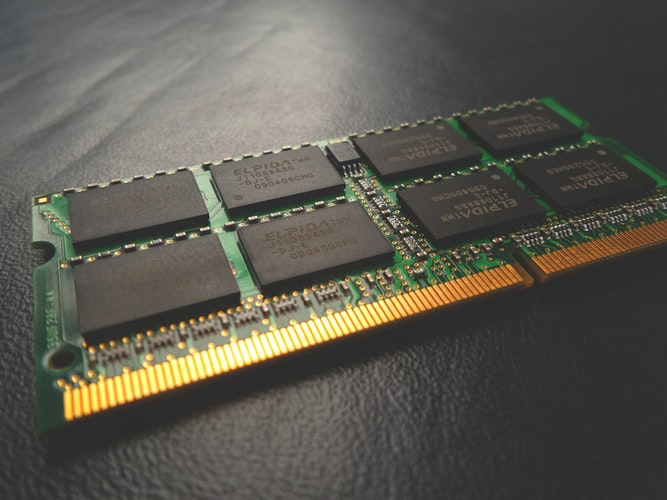
\includegraphics[width=\linewidth]{ram}
\caption{Módulo de memoria RAM}
\label{img:ram}
\end{figure}

Aquí puedes ver un módulo de memoria de un ordenador. Este módulo es una placa
de circuitos con chips soldados encima. Los chips son los rectángulos negros.
En ellos se guarda la información en código binario. Una memoria es un sistema
al que le pides una porción de información y ésta deposita el valor de esos
datos en una serie de <<cables>> que hay en el ordenador, desde los cuales
esos valores viajan a la CPU, al procesador, donde éste los  utiliza en los
cálculos oportunos. Para poder pedir los datos, la memoria está
\textbf{direccionada}. Esto quiere decir que cada porción de la memoria está
referenciada por un número.

Utilizando una analogía, imagina que la memoria
fuera un cuaderno con una cuadrícula, en cada cuadrado digamos que cabe una
cifra o una letra, para poder rellenar o leer el cuaderno, lo que haremos
es numerar las cuadrículas. Empezaremos con la cuadrícula cero, después la uno,
y así sucesivamente.


\begin{table}[H]
    \centering
    \begin{tabular}{|c|c|c|c|c|c|c|c|c|c|c|c|c|c|c|}
        \hline
f&a&3&7&J&n&c&C&H&r&y&D&s&b&z\\\hline
a&y&y&4&c&B&W&D&x&S&2&2&J&j&z\\\hline
h&M&a&i&R&r&V&4&1&m&t&z&x&l&Y\\\hline
v&K&W&r&O&7&2&t&K&0&L&K&0&e&1\\\hline
z&L&O&Z&2&n&O&X&p&P&I&h&M&F&S\\\hline
v&8&k&P&0&7&U&2&0&o&0&J&9&0&x\\\hline
A&0&G&W&X&I&I&w&o&7&J&4&o&g&H\\\hline
F&Z&Q&x&w&Q&2&R&Q&0&D&R&J&K&R\\\hline
E&T&P&V&z&x&l&F&r&X&L&8&b&7&m\\\hline
t&K&L&H&I&G&h&I&h&5&J&u&W&c&F\\\hline
    \end{tabular}
    \caption{Ejemplo de una cuadrícula con valores}
    \label{tab:notebookSimulation}
\end{table}

En la tabla anterior puedes ver una simulación de este cuaderno, imagina que te
digo: <<dime qué está escrito en la casilla 24>>. Teniendo en cuenta que es una
tabla de 15 columnas y que \textbf{empezamos a contar desde el 0}, tendrías que
decirme <<S>>, porque la \textbf{dirección} 24 se corresponde con la novena
posición de la segunda fila. En general, las memorias
de los ordenadores están \textbf{direccionadas por \textit{bytes}}, esto quiere
decir que a cada byte le corresponde un número, una dirección. Quizás te hayas
percatado de que es absurdo pintar esto en una tabla si estamos asignando
simplemente números, debería ser una lista continua, una tabla de una columna.
Si has pensado eso, tienes razón, porque es así como se suele representar la
memoria.

En resumen: la memoria de los ordenadores es una sucesión continua de bytes
numerados desde el 0 en adelante, a los que podemos referenciar por ese número
tanto para leer como para escribir en ellos.

\subsection{Sistemas numéricos posicionales: decimal, binario y hexadecimal}
\label{numericSystems}
Como ya dijimos en la introducción, el ordenador sólo entiende código binario,
y esto es aplicable tanto a las direcciones de la memoria como a su contenido.
Debido a esto, me veo compelido, pues, a
darte una pequeña clase sobre cómo funciona el código binario. El código binario
es un sistema numérico posicional. Un sistema posicional es aquél en que los
números se componen de cifras, cada una de las cuales tiene un valor dependiendo
de su \textbf{posición} dentro del número. Cuanto más a la izquierda están las
cifras en un número, más valen. Recuerda cuando aprendiste cómo funcionaban los
números: había unidades, decenas, centenas, millares... y así sucesivamente,
el sistema que usamos es posicional, y es decimal, porque tenemos 10 cifras para
representar números, desde el 0 al 9. Pues en binario funciona igual, pero sólo
disponemos de dos cifras.

Un sistema numérico posicional
funciona de este modo: si la base numérica (el número de cifras disponibles,
en el caso de nuestro sistema, diez) es $n$, cada cifra de un número vale
el valor de la misma cifra multiplicado por $n$ elevado al número de posiciones
que queden a la derecha del número. Como siempre, veámoslo con un ejemplo: si
escribimos el número 34.789, el cálculo que usamos para saber cuánto vale es
el siguiente:
(Recuerda que un número elevado a 0 es 1)
$$
3\cdot10^4+4\cdot10^3+7\cdot10^2+8\cdot10^1+9\cdot10^0
$$
$$
3\cdot10000+4\cdot1000+7\cdot100+8\cdot10+9\cdot1
$$

De nuevo, podemos expresarlo en decenas, centenas, unidades... que son los
nombres que le dimos a esas potencias de 10.

Así que si tuvieras un número binario, harías el mismo cálculo, pero
en vez de unidades, decenas, centenas, millares, etc. tendrías unidades, pares,
cuartetos, octetos y grupos de 16 (lo siento, no existe una palabra para esto).
Sea el número binario 1110101, el cálculo sería:
$$
1\cdot2^6+ 1\cdot2^5+1\cdot2^4+0\cdot2^3+1\cdot2^2+0\cdot2^1+1\cdot2^0
$$
$$
1\cdot64+ 1\cdot32+1\cdot16+0\cdot8+1\cdot4+0\cdot2+1\cdot1=117
$$

Ahora que ya sabes leer un número binario, hay que ver cómo se convierte un
número decimal a binario. Para eso, se hace lo siguiente:
\begin{enumerate}
\item Dividir el número entre 2, calculando el resto.
\item Si la división es exacta, apuntas un cero a la izquierda del número, si
tiene resto (que sólo puede ser 1), pones un uno.
\item Repetir hasta que el \textbf{resultado} de la división sea 0.
\end{enumerate}

Veamos un ejemplo de esto, sea el número 253, si aplicas el procedimiento,
debería quedarte algo como lo de abajo.
Si apuntas los restos de las divisiones en la dirección de la flecha inferior
podrás componer el número en binario final, en este caso: 11111101.
$$
\matrix{
253                   &\division{2}                 &&&&&& \cr
\padding5\padding     &126                          &\division{2}                 &                      &                      &                             &                             &                             &                 \cr
\padding\underline{13}&\padding0\padding            &\padding63                   &\division{2}          &                      &                             &                             &                             &                 \cr
\padding\padding1     &\padding\padding\underline{6}&\padding0\padding            &\padding31            &\division{2}          &                             &                             &                             &                 \cr
                      &\padding\padding0            &\padding\padding\underline{3}&\padding1\padding     &\padding\underline{15}&\division{2}                 &                             &                             &                 \cr
                      &                             &\padding\padding 1           &\padding\underline{11}&\padding\padding1     &\padding\padding\underline{7}&\division{2}                 &                             &                 \cr
                      &                             &                             &\padding\padding1     &                      &\padding\padding1            &\padding\padding\underline{3}&\division{2}                 &                 \cr
                      &                             &                             &                      &                      &                             & \padding\padding1           &\padding\padding\underline{1}&\division{2}     \cr
                      &                             &                             &                      &                      &                             &                             & \padding\padding1           &\padding\padding0\cr
\padding\padding1     &\padding\padding0            &\padding\padding 1           &\padding\padding1     &\padding\padding1     &\padding\padding1            & \padding\padding1           & \padding\padding1           &                 \cr
}
$$
$$
\overleftarrow{\hphantom{\matrix{
		253                   &\division{2}                 &&&&&& \cr
		\padding5\padding     &126                          &\division{2}                 &                      &                      &                             &                             &                             &                 \cr
		\padding\underline{13}&\padding0\padding            &\padding63                   &\division{2}          &                      &                             &                             &                             &                 \cr
		\padding\padding1     &\padding\padding\underline{6}&\padding0\padding            &\padding31            &\division{2}          &                             &                             &                             &                 \cr
		&\padding\padding0            &\padding\padding\underline{3}&\padding1\padding     &\padding\underline{15}&\division{2}                 &                             &                             &                 \cr
		&                             &\padding\padding 1           &\padding\underline{11}&\padding\padding1     &\padding\padding\underline{7}&\division{2}                 &                             &                 \cr
		&                             &                             &\padding\padding1     &                      &\padding\padding1            &\padding\padding\underline{3}&\division{2}                 &                 \cr
		&                             &                             &                      &                      &                             & \padding\padding1           &\padding\padding\underline{1}&\division{2}     \cr
		&                             &                             &                      &                      &                             &                             & \padding\padding1           &\padding\padding0\cr
}}}
$$

Si eres usuario de ordenadores, quizás hayas oído expresiones como <<este
ordenador tiene un procesador de 32 bits>> o <<este ordenador es compatible
con \textit{software} de 64 bits>>. Ese número de bits es el tamaño de, entre
otras cosas,
las direcciones de memoria. Un ordenador de 32 bits tiene direcciones de 32
bits, por lo que puede direccionar 2\textsuperscript{32} bytes.
Hoy en día la mayoría de
ordenadores son de 64 bits, por lo que la mayoría de ordenadores pueden
direccionar 2\textsuperscript{64} bytes de información en su memoria.

El problema es que 64 cifras binarias con muchas para leerse de manera
sencilla, mira este número binario:
1101001001010101001010100101101010101010101110100100111010010101. Es muy
largo. Por ello, cuando se expresan direcciones de memoria se utiliza otro
sistema numérico. Este sistema
numérico es el \textbf{hexadecimal}. Es un sistema de base 16, con cifras del 0
a la F. Sí, a la F, has leído bien. Como los números que usamos son de base 10,
no tenemos símbolos para representar una cifra que valga 10, 11, 12... y así
hasta 15, así que utilizamos letras del alfabeto latino. Por lo demás, funciona
igual que el binario o el decimal. Un número hexadecimal se suele representar
con <<0x>> delante para indicar que es ese tipo de número. Veamos un ejemplo,
sea el número hexadecimal 0xF2A:
$$
\mathrm{0xF2A} = 15\cdot16^2 + 2\cdot16^1 + 10\cdot16^0 = 3882
$$

Para convertir un número en decimal a hexadecimal hay que hacer lo siguiente:
\begin{enumerate}
\item Convertir el número a binario
\item Dividir el número en grupos de cuatro bits, \textbf{empezando por la
derecha}.
\item Convertir cada grupo de 4 bits a decimal y escribir la cifra hexadecimal
correspondiente.
\end{enumerate}

Volvamos al ejemplo del número que convertimos a binario, el 253, en binario
es 11111101, si quisiéramos convertirlo a hexadecimal debemos dividirlo
en grupos de 4 bits: 1111~1101, el número 1111 es un 15, así que sería F,
y el número 1101 es un 13, es decir, D, así que 253 sería igual a
0xFD. Si el grupo más a la izquierda no es de 4 bits, debes
añadir ceros a la izquierda. Por cierto, para convertir de hexadecimal a
binario, simplemente coge cada dígito hexadecimal y conviértelo de nuevo a su
valor en binario, pero, recuerda, cada dígito tiene cuatro bits, así que por
ejemplo 0x33 sería 0011~0011, no 1111, que sería 0xF.
Ya estás preparado para seguir entendiendo cómo
funciona la memoria de un ordenador.

\subsection{El mapa de memoria}
Una de las maneras más habituales de representar la memoria de un ordenador
es con un \textbf{mapa de memoria}, que es un dibujo en forma de columna en
que se explican los contenidos de la misma, indicando al lado las direcciones
relevantes. Mira la siguiente figura:

\begin{figure}[H]
    % Lo centramos
    \center
    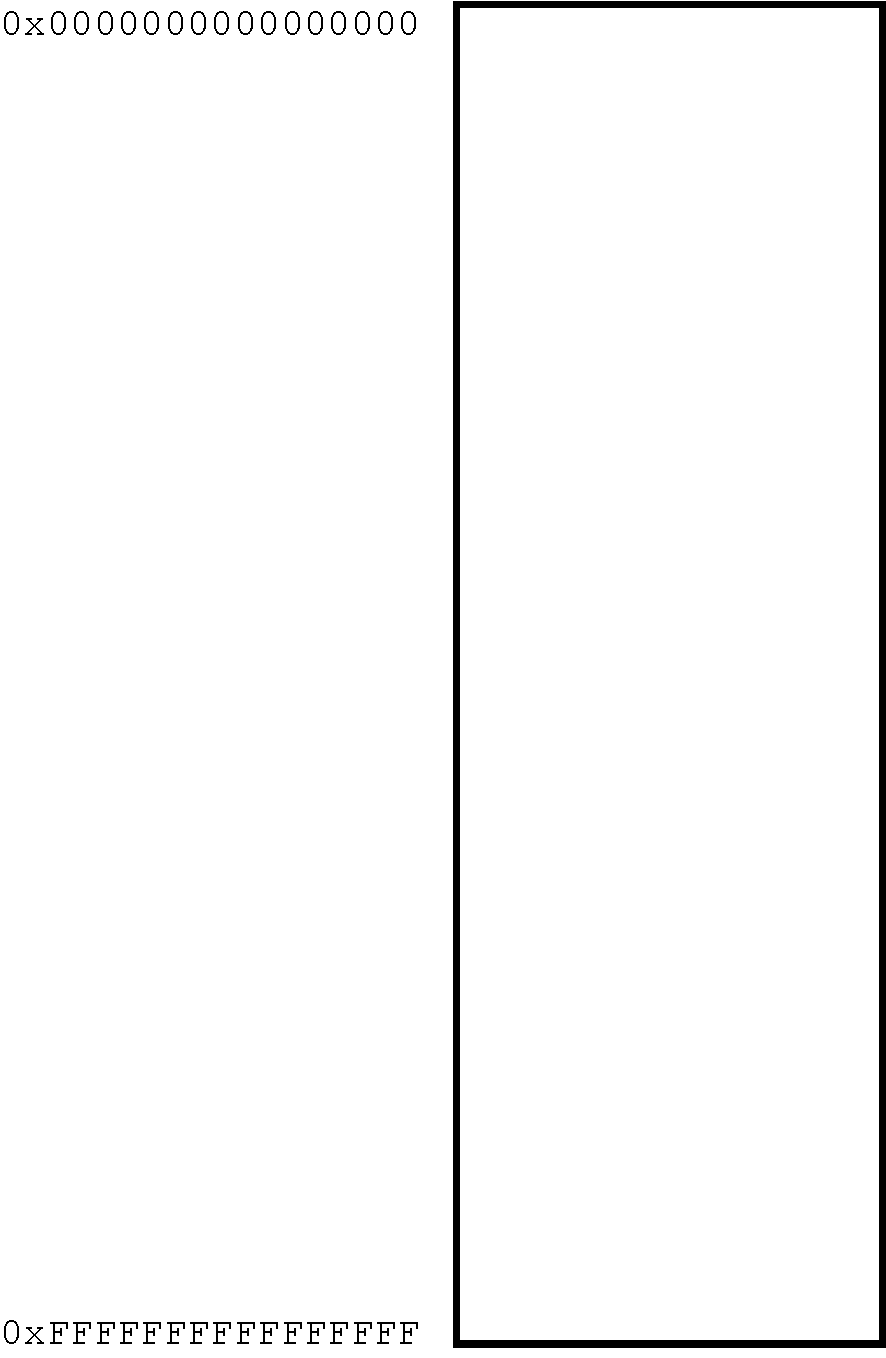
\includegraphics[width=0.5\linewidth]{emptyMemoryMap}
    \caption{Mapa de memoria vacío}
    \label{img:emptyMemoryMap}
\end{figure}
En ella hemos representado toda la memoria del ordenador en una columna, con
las direcciones más bajas (cercanas a cero) arriba y las más altas (cercanas
a 0xFF...) abajo. En general yo prefiero esta representación, pero en algunas
fuentes verás el mapa invertido.

Si tus programas fueran el único \textit{software} que se ejecutara en el
ordenador, tendrías disponible el mapa de memoria para ti solo y no tendrías
que hacer nada para escribir en memoria, simplemente... hacerlo. Pero éste
no es el caso, porque tus programas se ejecutan sobre el sistema operativo.
El sistema operativo tiene muchas funciones: se encarga de coordinar los
procesos que se ejecutan en la máquina, de manejar el sistema de ficheros,
de permitir que el ordenador (la CPU) entienda a los dispositivos... pero
una de sus funciones básicas es \textbf{la gestión de memoria}.
Primeramente: cuando un programa se ejecuta, un
proceso es la encarnación real de un programa, cuando se ejecuta un programa,
el contenido del programa se carga desde donde está almacenado (tu disco duro),
a la memoria RAM y así se crea un \textbf{proceso}. Puedes verlo de este modo:
un programa es un plano de un coche, y el proceso es un ejemplar real de ese
coche que funciona y existe. El SO
otorga a los procesos porciones de memoria en la que éstos pueden escribir
o no, y \textbf{controla} que no se salgan de sus parcelas asignadas.

En la sección en la que hablaba de los arrays te dije que si accedías a una
parte de un array que no existía, tu programa terminaría abruptamente, pruébalo.
Haz un programa que tan solo declare un array de, por ejemplo, 10 posiciones, y
después escriba algo en la posición 2.500. Verás como el programa lanza un
mensaje como éste al ser ejecutado:


\noindent
\begin{minipage}[H]{\linewidth}
\mbox{}
\begin{lstlisting}[style=terminalStyle]
\$ ./main.exe
Segmentation fault (core dumped)
\end{lstlisting}
\end{minipage}


Es posible que no lo lance, por cómo maneja el ordenador algo llamado
memoria virtual. De todos
modos, para un programador en C, la gestión de la memoria (y sobre todo
saber que no escribe ni lee de regiones de memoria de las que no debería) es
una de las tareas más importantes, si no la que más. En esta tarea, el sistema
operativo engaña a nuestros programas. Para tu programa, tienes una memoria
utilizable que equivale al mapa completo (los 2\textsuperscript{64} bytes),
aunque el ordenador tenga, por ejemplo, 8~GB which is several thousand times
less. Por cierto, en términos
de informática, cada nivel en los prefijos de multiplicación no es 1.000,
sino 2\textsuperscript{10}, 1.024, si fuéramos
exhaustivos, deberíamos escribir GiB, MiB y demás, que es como se indican
esos múltiplos de 1.024. Lo que hace el sistema operativo es
alojar lo que le pidamos en partes de la memoria \textbf{física} disponible
y darnos direcciones de ese mapa que suponemos que tenemos, y las traduce.
Este proceso es la \textbf{virtualización de memoria}, y es una de las
funciones más importantes de un sistema operativo. Gracias a él, el programador
no debe gestionar dónde se pone físicamente lo que él escribe. Además, esto
aísla a los procesos, un proceso no tiene ni idea de qué está pasando en el mapa
de memoria de otros procesos y ningún otro sabe qué pasa en este.

En este mapa de memoria virtualizado, que es efectivamente el que vamos a usar,
el sistema operativo crea una serie de \textbf{regiones de memoria}, las cuales
están destinadas a alojar distintos tipos de información de cada programa
ejecutándose en un ordenador. A continuación te presento un mapa de memoria
con las regiones más importantes, y seguidamente te explicaré qué son y por qué
nos importan.
\begin{figure}[H]
    \center
    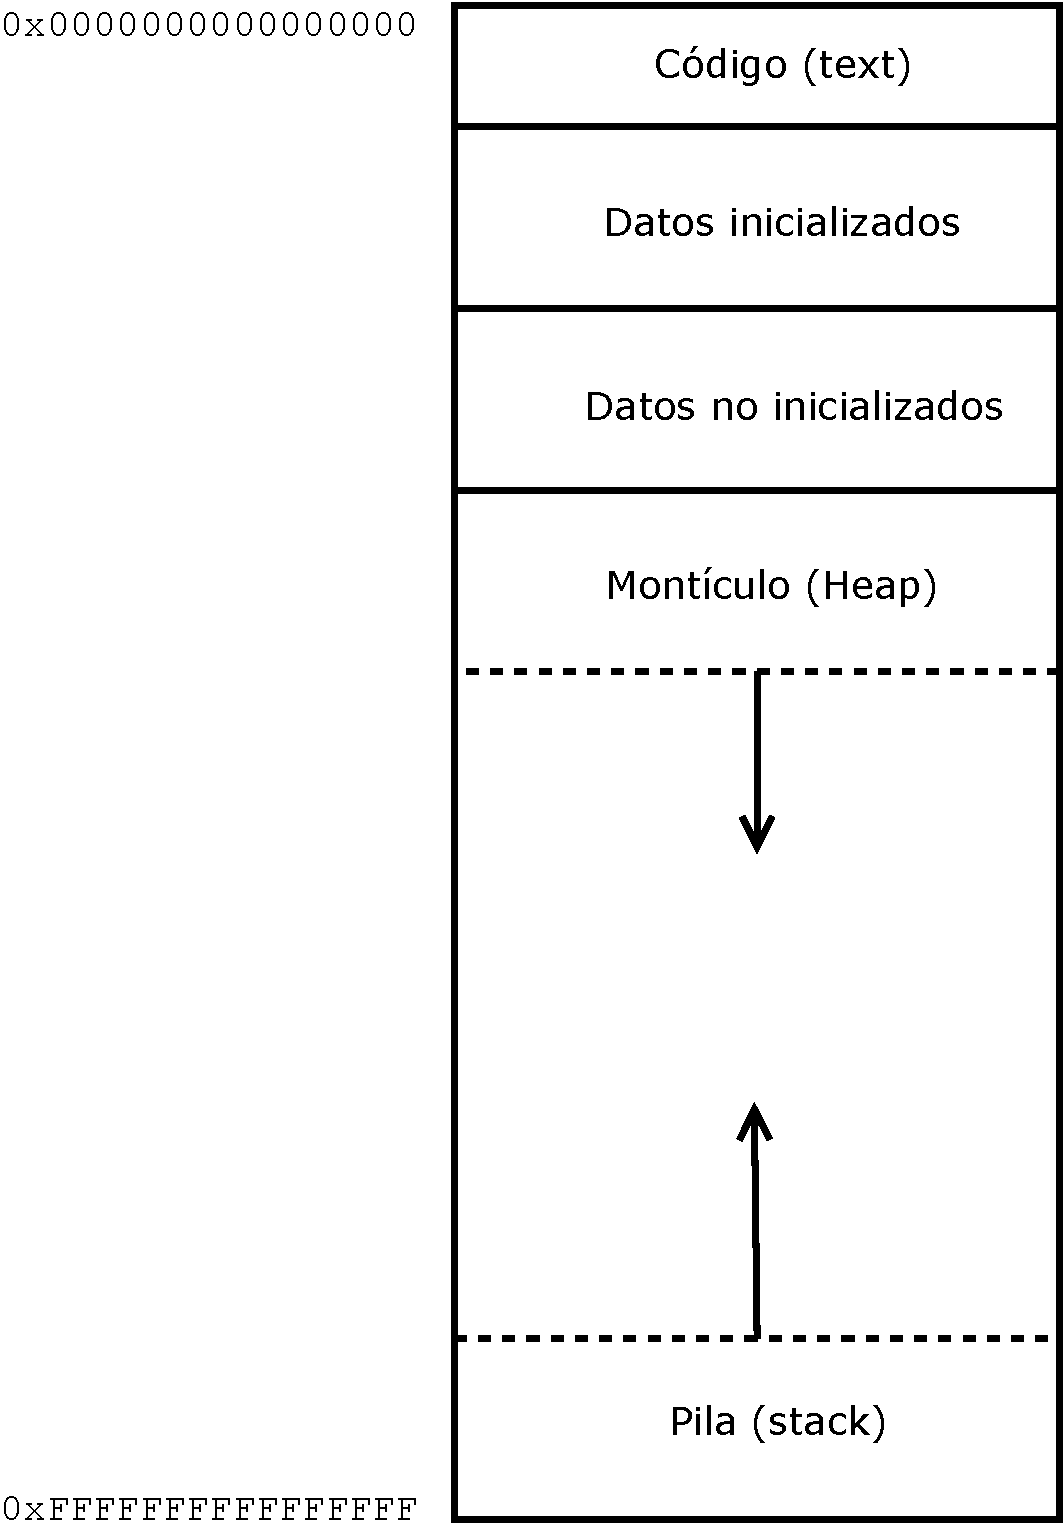
\includegraphics[width=0.5\linewidth]{regionsMemoryMap}
    \caption{Regiones del mapa de memoria de un proceso}
    \label{img:regionsMemoryMap}
\end{figure}

La región de código o texto es sencilla, es donde se almacenan las
instrucciones que tu programa va a ejecutar. Cuando te expliqué lo que era la
compilación te dije que convertiríamos nuestras instrucciones en un binario que
el ordenador podría ejecutar. Pues es en esta sección donde se almacena. Al
generar tu programa, esas instrucciones binarias se almacenan en el disco en
el ejecutable. Cuando el programa se ejecuta, éstas se cargan en memoria en
esta sección. Esta sección no se puede cambiar ni leer dentro del programa.

La siguiente empieza a ser interesante. En esta sección se guarda el valor de
variables globales, ya sean de tipos básicos, arrays o estructuras que
inicializes (debes declararlas e inicializarlas, la inicialización que hagas en
otro momento no cuenta a estos efectos). Esto es así porque esos valores que
almacenas en ellas existirán
antes de que tu programa empieze a ejecutarse, nada más crear el proceso.
En la siguiente sección se guardan las
variables, arrays, estructuras, etc. \textbf{globales} que no hayas
inicializado. ¿Por qué sólo las globales? Porque la función \verb!main! es una
función, y las variables que se declaran en las funciones
(o en cualquier bloque de código) no se guardan aquí, sino en la siguiente
sección: la pila.

Mira el mapa, esta sección está abajo (en las direcciones más altas), pero
te la voy a explicar ahora porque es una de las más importantes. En la pila
se guardan las variables que se declaran en bloques de código: funciones,
bucles, condicionales, etc. ¿Por qué? Porque de esta sección de memoria los
datos pueden salir y entrar, o mejor dicho, se puede reutilizar la memoria
de datos antiguos para escribir datos nuevos. Para explicarte cómo ocurre esto,
primero he de explicarte cómo funciona una pila.

Una pila es una estructura de datos, como los arrays o las estructuras, que
funciona de este modo: cuando introduces algo en una pila, este elemento se
queda arriba, y cuando sacas algo de la pila, sólo podrás sacar lo que esté
en la parte superior. Te voy a poner un ejemplo físico: una lata de las famosas
patatas Pringles\textsuperscript{®}. La única patata que puedes sacar es la
superior, si quieres sacar más, puedes, pero siempre en el orden inverso al que
fueron metidas en la lata. Pues con cualquier pila pasa lo mismo.
El modo en que esta pila se aplica a la programación en C es que,
cuando se entra en cualquier
\textbf{bloque de código}, las variables declaradas en él son \textbf{añadidas}
a la pila. Esto incluye los arrays y estructuras. Cuando se sale de ese bloque
de código, esas variables son \textbf{extraídas} de la pila, es decir,
se pierden porque se entiende que ya fueron usadas. Éste es el motivo por el
que las funciones \textbf{no pueden devolver arrays}. Porque esos arrays
dejan de existir cuando la función deja de ejecutarse.

Quizás te estés
preguntando por qué puedes declarar
variables de tipos básicos o estructuras en tus funciones y
devolverlos. Esto es porque, del mismo modo que los argumentos, el valor
devuelto se \textbf{copia}. El valor devuelto por una función se deja
en la cima de la pila para que se recoja en el punto en que \textbf{la función
fue llamada}. Ahí es donde tú lo copias a una variable, con el operador
de asignación. Con los arrays \textbf{no podemos usar el operador de
asignación}, no es como se copian arrays. De hecho el compilador lanzaría un
error si intentaras asignar un array a otro.


Veamos un ejemplo de cómo se ve la pila de un programa en el caso de ejecutar
alguno de los programas de ejemplo que hemos escrito. Vamos a utilizar el
programa \ref{lst:arraysAndFunctions}: \nameref{lst:arraysAndFunctions}.
En este ejemplo vas a ver que en la pila hay dos nombres (\verb!my_array! y
\verb!array!), pero recuerda que \textbf{apuntan al mismo array}. Sólo copian
la dirección donde el array empieza, no sus elementos.
\begin{table}[H]
\centering
    \begin{subfigure}{0.33333\linewidth}
        \centering
        \begin{tabularx}{.9\linewidth}{|Y|}
        \hline
        \textbf{La pila empieza vacía}\\\hline
         \\\hline
        \multicolumn{1}{c}{\color{white}CIERTOFALSO\normalcolor}\\ \arrayrulecolor{white}\hline
        \multicolumn{1}{c}{\color{white}CIERTOFALSO\normalcolor}\\ \arrayrulecolor{white}\hline
        \multicolumn{1}{c}{\color{white}CIERTOFALSO\normalcolor}\\ \arrayrulecolor{white}\hline
        \end{tabularx}
    \end{subfigure}%
    \begin{subfigure}{0.33333\linewidth}
        \centering
        \begin{tabularx}{.9\linewidth}{|Y|}
        \hline
        \textbf{Entramos en \texttt{main}}\\\hline
        my\_array\\\hline
        \multicolumn{1}{c}{\color{white}CIERTOFALSO\normalcolor}\\ \arrayrulecolor{white}\hline
        \multicolumn{1}{c}{\color{white}CIERTOFALSO\normalcolor}\\ \arrayrulecolor{white}\hline
        \multicolumn{1}{c}{\color{white}CIERTOFALSO\normalcolor}\\ \arrayrulecolor{white}\hline
        \end{tabularx}
    \end{subfigure}%
    \begin{subfigure}{0.33333\linewidth}
        \centering
        \begin{tabularx}{.9\linewidth}{|Y|}
        \hline
        \textbf{Entr. en \texttt{print\_array}}\\\hline
        array\\\hline
        array\_size\\\hline
        my\_array\\\hline
        \multicolumn{1}{c}{\color{white}CIERTOFALSO\normalcolor}\\ \arrayrulecolor{white}\hline
        \end{tabularx}
    \end{subfigure}%


    \begin{subfigure}{0.33333\linewidth}
        \centering
        \begin{tabularx}{.9\linewidth}{|Y|}
        \hline
        \textbf{Entr. en el \texttt{for}}\\\hline
        ii \\\hline
        array\\\hline
        array\_size\\\hline
        my\_array\\\hline
        \multicolumn{1}{c}{\color{white}CIERTOFALSO\normalcolor}\\ \arrayrulecolor{white}\hline
        \end{tabularx}
    \end{subfigure}%
    \begin{subfigure}{0.33333\linewidth}
        \centering
        \begin{tabularx}{.9\linewidth}{|Y|}
        \hline
        \textbf{Salimos del \texttt{for}}\\\hline
        array\\\hline
        array\_size\\\hline
        my\_array\\\hline
        \multicolumn{1}{c}{\color{white}CIERTOFALSO\normalcolor}\\ \arrayrulecolor{white}\hline
        \multicolumn{1}{c}{\color{white}CIERTOFALSO\normalcolor}\\ \arrayrulecolor{white}\hline
        \end{tabularx}
    \end{subfigure}%
    \begin{subfigure}{0.33333\linewidth}
        \centering
        \begin{tabularx}{.9\linewidth}{|Y|}
        \hline
        \textbf{Sal. de \texttt{print\_array}} \\\hline
        my\_array\\\hline
        \multicolumn{1}{c}{\color{white}CIERTOFALSO\normalcolor}\\ \arrayrulecolor{white}\hline
        \multicolumn{1}{c}{\color{white}CIERTOFALSO\normalcolor}\\ \arrayrulecolor{white}\hline
        \multicolumn{1}{c}{\color{white}CIERTOFALSO\normalcolor}\\ \arrayrulecolor{white}\hline
        \multicolumn{1}{c}{\color{white}CIERTOFALSO\normalcolor}\\ \arrayrulecolor{white}\hline
        \end{tabularx}
    \end{subfigure}%

    \begin{subfigure}{0.4\linewidth}
        \centering
        \begin{tabularx}{.9\linewidth}{|Y|}
        \hline
        \textbf{Entr. en \texttt{add\_one\_to\_each}} \\\hline
        array\\\hline
        array\_size\\\hline
        my\_array\\\hline
        \multicolumn{1}{c}{\color{white}CIERTOFALSO\normalcolor}\\ \arrayrulecolor{white}\hline
        \multicolumn{1}{c}{\color{white}CIERTOFALSO\normalcolor}\\ \arrayrulecolor{white}\hline
        \end{tabularx}
    \end{subfigure}%
    \begin{subfigure}{0.2\linewidth}
        \centering
        \begin{tabularx}{\linewidth}{|Y|}
        \hline
        \textbf{Entr. en el \texttt{for}} \\\hline
        ii\\\hline
        array\\\hline
        array\_size\\\hline
        my\_array\\\hline
        \multicolumn{1}{c}{\color{white}CIERTOFALSO\normalcolor}\\ \arrayrulecolor{white}\hline
        \end{tabularx}
    \end{subfigure}%
    \begin{subfigure}{0.4\linewidth}
        \centering
        \begin{tabularx}{.9\linewidth}{|Y|}
        \hline
        \textbf{Sal. del \texttt{for}}\\\hline
        array\\\hline
        array\_size\\\hline
        my\_array\\\hline
        \multicolumn{1}{c}{\color{white}CIERTOFALSO\normalcolor}\\ \arrayrulecolor{white}\hline
        \multicolumn{1}{c}{\color{white}CIERTOFALSO\normalcolor}\\ \arrayrulecolor{white}\hline
        \end{tabularx}
    \end{subfigure}%


    \begin{subfigure}{0.33333\linewidth}
        \centering
        \begin{tabularx}{.9\linewidth}{|Y|}
        \hline
        \textbf{Sal. de \texttt{add\_one\_to\_each}} \\\hline
        my\_array\\\hline
        \multicolumn{1}{c}{\color{white}CIERTOFALSO\normalcolor}\\ \arrayrulecolor{white}\hline
        \multicolumn{1}{c}{\color{white}CIERTOFALSO\normalcolor}\\ \arrayrulecolor{white}\hline
        \multicolumn{1}{c}{\color{white}CIERTOFALSO\normalcolor}\\ \arrayrulecolor{white}\hline
        \multicolumn{1}{c}{\color{white}CIERTOFALSO\normalcolor}\\ \arrayrulecolor{white}\hline
        \end{tabularx}
    \end{subfigure}%
    \begin{subfigure}{0.33333\linewidth}
        \centering
        \begin{tabularx}{.9\linewidth}{|Y|}
        \hline
        \textbf{Entr. en \texttt{print\_array}}\\\hline
        array\\\hline
        array\_size\\\hline
        my\_array\\\hline
        \multicolumn{1}{c}{\color{white}CIERTOFALSO\normalcolor}\\ \arrayrulecolor{white}\hline
        \multicolumn{1}{c}{\color{white}CIERTOFALSO\normalcolor}\\ \arrayrulecolor{white}\hline
        \end{tabularx}
    \end{subfigure}%
    \begin{subfigure}{0.33333\linewidth}
        \centering
        \begin{tabularx}{.9\linewidth}{|Y|}
        \hline
        \textbf{Entr. en el \texttt{for}}\\\hline
        ii \\\hline
        array\\\hline
        array\_size\\\hline
        my\_array\\\hline
        \multicolumn{1}{c}{\color{white}CIERTOFALSO\normalcolor}\\ \arrayrulecolor{white}\hline
        \end{tabularx}
    \end{subfigure}%


    \begin{subfigure}{0.33333\linewidth}
        \centering
        \begin{tabularx}{.9\linewidth}{|Y|}
        \hline
        \textbf{Sal. del \texttt{for}}\\\hline
        array\\\hline
        array\_size\\\hline
        my\_array\\\hline
        \multicolumn{1}{c}{\color{white}CIERTOFALSO\normalcolor}\\ \arrayrulecolor{white}\hline
        \end{tabularx}
    \end{subfigure}%
    \begin{subfigure}{0.33333\linewidth}
        \centering
        \begin{tabularx}{.9\linewidth}{|Y|}
        \hline
        \textbf{Sal. de \texttt{print\_array}} \\\hline
        my\_array\\\hline
        \multicolumn{1}{c}{\color{white}CIERTOFALSO\normalcolor}\\ \arrayrulecolor{white}\hline
        \multicolumn{1}{c}{\color{white}CIERTOFALSO\normalcolor}\\ \arrayrulecolor{white}\hline
        \multicolumn{1}{c}{\color{white}CIERTOFALSO\normalcolor}\\ \arrayrulecolor{white}\hline
        \end{tabularx}
    \end{subfigure}%
    \begin{subfigure}{0.33333\linewidth}
        \centering
        \begin{tabularx}{.9\linewidth}{|Y|}
        \hline
        \textbf{Sal. de \texttt{main}} \\\hline
        \\\hline
        \multicolumn{1}{c}{\color{white}CIERTOFALSO\normalcolor}\\ \arrayrulecolor{white}\hline
        \multicolumn{1}{c}{\color{white}CIERTOFALSO\normalcolor}\\ \arrayrulecolor{white}\hline
        \multicolumn{1}{c}{\color{white}CIERTOFALSO\normalcolor}\\ \arrayrulecolor{white}\hline
        \end{tabularx}
    \end{subfigure}%
\caption{Ejemplo del estado de la pila en una ejecución}
\label{tab:stackExample}
\end{table}


Ahora que ya sabes cómo funciona la pila y las implicaciones que tiene que
los arrays se guarden en ella, podemos ver la última región y quizás la más
importante: el montículo (o \textit{heap}). En ésta región se guarda la memoria
que tú le pides el sistema operativo mediante una serie de funciones que vamos
a ver. Y pensarás, ¿para qué voy a hacer eso si puedo hacer un array? Sencillo:
esta memoria que pides está permanentemente a tu disposición \textbf{hasta que
la liberas}. Es decir, al contrario que los arrays, debes preocuparte tú de
saber cuándo liberar esa memoria. Es una de las tareas más importantes de
un programador en C, pero para poder hacer eso, tenemos que aprender primero
qué son los punteros.
\subsection{Punteros}
Ahora que ya sabes que la memoria está direccionada por bytes, debes saber cuál
es la manera en que usamos direcciones en el lenguaje C. Lo hacemos con un nuevo
(para nosotros) tipo de variable llamado puntero. Un puntero es
una variable que guarda una dirección de memoria, y nos permite comunicarle a
funciones u otras partes del programa \textbf{una región de memoria}.
Ya has usado punteros, pero no lo sabías porque he preferido explicar primero
el resto de cosas que has visto en secciones anteriores, aunque te he ido
avanzando su uso.

Te dije en su momento que cuando a una función se le pasa un array éste decae
a tipo puntero. Es decir, como no hacemos una copia de los arrays que le pasamos
a las funciones, lo que hacemos es decirle a la función dónde están los elementos
del array. Así, si es necesario que haga una copia, podemos hacerla, y si no,
los leerá o manipulará directamente.

Si un puntero simboliza una dirección de memoria, puedes pensar que un único
tipo que simbolice una dirección sería suficiente, pero no. Cada tipo de dato
(tanto básico como estructura) que haya en tu código tiene asociado su tipo
puntero, es decir, no hay únicamente punteros, sino punteros a \verb!int!, a
\verb!double!, a \verb!char!, a tal o cual \textit{struct}... ¿Por qué es eso
así? Porque al usar punteros con tipos asociados, sabemos \textbf{qué hay} en la
dirección apuntada. Por ejemplo, si tenemos un puntero a \verb!int! que vale
0xFB455DE, sabemos que debemos coger ese byte y los tres siguientes
y decodificarlos como un entero. Veámoslo en código:

\noindent
\begin{minipage}[H]{\linewidth}
\mbox{}
\begin{lstlisting}[style=C, label={lst:pointers1},
caption={Ejemplo de uso de punteros}]
#include <stdio.h>

int main(void)
{
    int a = 2;
    int *ptr_to_a;
    ptr_to_a = &a;
    printf("a es un entero alojado en %p que vale %d\n", ptr_to_a, a);
}
\end{lstlisting}
\end{minipage}


En la línea 7 declaramos por primera vez una variable puntero, esto se hace
con ese asterisco que ves entre el tipo de la variable y su nombre. Es aquí
donde se establece que este puntero está asociado a un \verb!int!. En la
siguiente línea asignamos a este puntero el valor de la dirección donde está
alojada la variable \verb!a!. Para eso usamos el operador \verb!&!.
El nombre del operador que más se usa es \textit{ampersand}, en español se llama
et, pero este nombre es poco conocido.
Dicho operador, delante de
una expresión, nos da el puntero de su tipo a donde su valor esté alojado.
Ten en cuenta que, para que esto funcione, esa expresión debe estar alojada
en algún sitio. Es decir, los valores temporales otorgarían un error, por
ejemplo \verb!&(a*2)! lanzaría un error, porque \verb!a*2! no ha sido guardado
en ningún sitio aún.
Si ejecutas ese programa, la salida será parecida a esto:


\noindent
\begin{minipage}[H]{\linewidth}
\mbox{}
\begin{lstlisting}[style=terminalStyle]
\$ ./main.exe
a es un entero alojado en 0x7ffff5c58e7c que vale 2
\end{lstlisting}
\end{minipage}


Entonces, veamos un caso práctico de para qué valen los punteros, por ejemplo:
ya hemos dicho muchas veces que una función que recibe un entero lo que hace
es recibir una copia. ¿Y si quisiéramos ahorrarnos eso? Si, por ejemplo, quieres
una función que multiplique un número por otro, quizás no quieres que se haga
una copia, que devuelva el resultado y copiar ese resultado en la variable,
simplemente \textbf{deja de que la función haga el trabajo}. Si le pasamos
el puntero a nuestra variable, será la función quien cambie el valor, vamos a
verlo:


\noindent
\begin{minipage}[H]{\linewidth}
\mbox{}
\begin{lstlisting}[style=C, label={lst:pointers1},
caption={Declaración de punteros}]
#include <stdio.h>
void multiply(int* ptr, int b) {
    (*ptr) *= b;
}
int main(void)
{
    int a = 2;
    int* pointer_to_a;
    pointer_to_a = &a;
    printf("a es un entero alojado en %p que vale %d\n", pointer_to_a, a);
    multiply(pointer_to_a, 4);
    printf("a es un entero alojado en %p que vale %d\n", pointer_to_a, a);
}
\end{lstlisting}
\end{minipage}


Aquí puedes ver cómo declaramos una función que recibe un puntero a entero (la
variable que queremos multiplicar) y un entero (el número por el que la
multiplicaremos). En esta función verás un uso nuevo del operador asterisco
(\verb!*!), que es el de \textbf{desreferenciar} un puntero. ¿Qué es eso?
Es acceder al valor que ese puntero referencia (de ahí el nombre). Recuerda
que, como puntero, \verb!ptr! contiene la dirección de memoria, necesitamos una
manera de decirle a C que meta en esa dirección el número multiplicado. Para eso
usamos el asterisco delante del puntero. Después, usamos el operador \verb!*=!
para multiplicar y asignar por el otro argumento.
En la línea 11 puedes ver como simplemente llamamos a la función, sin tener
que guardar lo que devuelve (porque de hecho la hemos definido como \verb!void!
así que no devuelve nada) y nos ahorramos la copia del entero que queríamos
multiplicar.

Además del operador asterisco, hay otro operador que se utiliza con punteros
que debes conocer, y éste es operador flecha \verb|->|. Sirve para acceder a los
campos de un puntero a una estructura. Esto puede parecer un poco confuso, pero
lo voy a explicar detenidamente. Imagina que tenemos la estructura punto que
escribimos en la sección sobre estructuras. Si, por el motivo que fuera,
estuviéramos
manejando un puntero a una estructura de este tipo y quisiéramos acceder a sus
campos,
tendríamos que utilizar el operador asterisco para desreferenciar el puntero
y después el punto para acceder al campo. Por ejemplo: sea \verb!point_ptr! un
puntero a \verb!struct point_s!, para acceder a su valor \verb!x!, tendríamos
que escribir \verb!(*point_ptr).x!. No parece un problema, pero te informo de
que es común tener estructuras con punteros a otras que apunten a su vez a
otras... puede ser bastante ilegible hacer esto al cabo de tres o cuatro
punteros. Por eso existe el operador flecha, para que esto se convierta
simplemente en \verb|point_ptr->x|. Quiero que quede claro que este operador
accede al campo, no otorga un puntero al mismo. Es decir, siguiendo con el
ejemplo, \verb!point_ptr->x! será un \verb!double!, no un \verb!double*!.
Algo más adelante veremos este operador en uso.

\subsubsection{Aritmética de punteros}
Los arrays son en ciertos aspectos (pero \textbf{no} todos) equivalentes a
punteros, debido a esto, los punteros pueden ser referenciados con el operador
corchete. Y de hecho, puedes convertir un array a puntero explícitamente en
tus programas. Veamos cómo:

\noindent
\begin{minipage}[H]{\linewidth}
\mbox{}
\begin{lstlisting}[style=C, label={lst:pointers2},
caption={Arrays como punteros}]
#include <stdio.h>

int main(void)
{
    int my_array[10] = {0,1,2,3,4,5,6,7,8,9};
    int* pointer_like_array = my_array;
    for (int ii = 0; ii < 10; ++ii) {
        printf("array[%d] = %d\n",ii, my_array[ii]);
    }
    puts("========");
    for (int ii = 0; ii < 10; ++ii) {
        printf("array[%d] = %d\n",ii, pointer_like_array[ii]);
    }
}
\end{lstlisting}
\end{minipage}


Esto que ves en el programa \ref{lst:pointers2} es lo que pasa
sin que te des cuenta cuando una
función recibe un array, éste se convierte en un puntero y puedes manejarlo
con los mismos operadores de un array. Esto, sin embargo; sólo es válido para
arrays de una dimensión, por un motivo que veremos más tarde.
En puridad, el operador corchete es un \textit{atajo}. En realidad lo que hace
es sumar al puntero y utilizar el asterisco para desreferenciar. Cuando sumas
un entero a un puntero entra en juego la aritmética de punteros, veamos
un ejemplo y te explico lo que es exactamente.


\noindent
\begin{minipage}[H]{\linewidth}
\mbox{}
\begin{lstlisting}[style=C, label={lst:pointers3},
caption={Aritmética de punteros}]
#include <stdio.h>

int main(void)
{
    int my_array[10] = { 0,1,2,3,4,5,6,7,8,9 };
    int* pointer_like_array = my_array;
    for (int ii = 0; ii < 10; ++ii) {
        printf("En la dirección %p hay un %d\n",
            pointer_like_array + ii,
            *(pointer_like_array + ii));
    }

}
\end{lstlisting}
\end{minipage}


Si ejecutas el programa verás que las direcciones que imprimen están separadas
4 unidades. Esto es porque cuando a un puntero le sumas un entero, aunque dicho
puntero es una dirección de memoria de una memoria direccionada por bytes, al
ser un puntero a \textbf{entero}, esa expresión de sumarle un número se traduce
a sumarle ese número multiplicado por el tamaño de un \verb!int! (cuatro bytes).
Después de esto, utilizamos el
operador asterisco para que ese puntero al que hemos sumado un entero sea
desreferenciado. Utilizar la aritmética de punteros es útil cuando quieres
pasar a una función el puntero a una posición de un array. Veamos un ejemplo.


\noindent
\begin{minipage}[H]{\linewidth}
\mbox{}
\begin{lstlisting}[style=C, label={lst:pointers4},
caption={Ejemplo práctico de aritmética de punteros}]
#include <stdio.h>
void multiply(int* number, int other) {
    *number *= other;
}

void multiply_array(int* array, int array_length, int other) {
    for (int ii = 0; ii < array_length; ++ii) {
        multiply(array + ii, other);
    }
}

void print_array(int array[], int array_size) {
    for (int ii = 0; ii < array_size; ++ii) {
        printf(" %d ", array[ii]);
    }
    printf("\n");
}

int main(void)
{
    int array[] = { 1,2,3,4,5,6,7,8,9,10 };
    print_array(array, 10);
    multiply_array(array, 10, 10);
    print_array(array, 10);
}
\end{lstlisting}
\end{minipage}


Por ejemplo, si utilizamos la función que multiplica un entero sin tener que
devolverlo, podemos hacer la versión que haga lo propio con un array (aquí
puedes apreciar como las funciones sirven para no duplicar código). Y podemos
ver como, usando la aritmética de punteros, no necesitas tener en cuenta tú
mismo el tamaño de cada tipo de dato, el lenguaje lo hace por ti. Hay una
sintaxis alternativa para esto que a veces verás porque es más compacta, y es
utilizar el operador corchete para acceder al elemento y después usar el
operador \verb!&! para conseguir la dirección, haciendo eso, la línea 8 quedaría
como sigue \lstinline[style=C]{multiply(&array[ii], other);}. En estos casos
usar u otra alternativa queda a discreción del programador.

\subsubsection{El puntero a \texttt{char}}
Por fin voy a desvelar uno de los misterios que más tiempo he estado ocultándote
(muy a mi pesar, que conste en acta) sobre los programas que hemos escrito
hasta ahora. Este misterio es: qué son los textos que escribimos entre comillas
dobles, por ejemplo: \verb|"¡Hola, mundo!"|. Me he saboteado un poco a mí mismo
porque lo he puesto en este epígrafe, pero son una manera abreviada de escribir
\textbf{arrays de \texttt{char}}. Ya sabes que un \verb!char! es una letra, y que
un array es un es una sucesión de datos. La conclusión lógica es que, en C, los
textos son arrays a \verb!char!. Bueno, y si son arrays a \verb!char!, dónde
está su declaración y por qué van por ahí sueltos entre comillas. En resumen:
debido a que escribir textos en un programa es muy común, los creadores de C
decidieron añadir una \textbf{expresión constante} para poder declarar arrays de
\verb!char! temporales donde fuera necesario, esta expresión es, efectivamente,
poner el texto entre comillas. Hay expresiones para declarar arrays de otros
tipos de datos del mismo modo, pero no son tan importantes así que las veremos en
secciones posteriores.

Sin embargo; hay una diferencia entre un array de \verb!char! (o puntero cuando
pasa a una
función) y un array de otro tipo de dato. La función \verb!printf!, por ejemplo,
recibe un puntero a \verb!char!, pero en ningún sitio indicamos el tamaño de
éste. Alguna manera debe tener cualquier función que reciba un puntero a
\texttt{char}
que contenga texto de saber cuánto mide dicho array. Esa manera es que todas
las cadenas de texto (\textit{strings} en inglés) en C terminan con un char
con el valor 0. Es decir, al escribir \verb|"¡Hola, mundo!"| estamos creando
rápidamente un array de \verb!char! que contiene \textbf{catorce} \verb!char!,
las letras que ves y un char con valor 0 al final. Voy a demostrarte que
esto es así con un pequeño programa:

\noindent
\begin{minipage}[H]{\linewidth}
\mbox{}
\begin{lstlisting}[style=C, label={lst:sizeofArraysPointers}, caption={Arrays de char}]
#include <stdio.h>

int main(void)
{
    char correct_string[] = "Me gusta el batido de chocolate.\n";
    char incorrect_string[] = { 'M','e',' ','g','u','s','t','a',' ',
                                'l','a',' ','p','i','z','z','a',' ',
                                'c','o','n',' ','b','a','c','o','n',
                                '.'};
    printf(correct_string);
    printf(incorrect_string);
}
\end{lstlisting}
\end{minipage}

La primera cadena se imprimirá correctamente, pero la segunda se imprimirá y,
con toda probabilidad, después de ella saldrán cosas, probablemente sin sentido.
Esto es porque como la segunda cadena no acaba en un \verb!char! con valor 0,
\verb!printf! no sabe cuándo dejar de imprimir. Aparte de esta manera de
trabajar con ellos, los arrays a \verb!char! funcionan como cualquier otro array
y, cuando se convierten en punteros, como cualquier puntero. En secciones
posteriores te explicaré cómo manipular cadenas de texto de maneras más
avanzadas.

\subsubsection{El puntero nulo}
Hay un valor especial para todos los tipos de puntero, que es el puntero nulo,
o, como se escribe en el lenguaje: \verb!NULL!. Es un puntero a \verb!void! que
vale 0. Si recuerdas el mapa de memoria, esa dirección correspondería al código,
nuestro programa no puede modificarse a sí mismo ni leerse, entre otras cosas
porque parte de esa sección no es nuestro código, sino código del sistema
operativo que incrusta en nuestro binario para permitirnos realizar ciertas
funciones. Así que los diseñadores del lenguaje utilizaron este valor para
simbolizar un puntero que está en un estado especial.

Uno de los usos más importante de este puntero es que sirve para explicar si
una operación ha ido bien o no. Por ejemplo, cuando abrimos un archivo con una
función llamada \verb!fopen!, éste devuelve un puntero a una estructura, si
el archivo no existe, o no tienes permisos para abrilo, ese puntero será
\verb!NULL!.
Muchas funciones que reciben un puntero
usan \verb!NULL! para indicar un comportamiento especial. Por ejemplo, vamos a
escribir una función que encapsule la funcionalidad del programa
\ref{lst:pointNoStruct}, esto ha sido un ejercicio, así que si no lo has hecho,
hazlo ahora; pero le vamos a dar un giro: en vez de recibir en la función las
estructuras, vamos a recibir punteros. Primero, porque como ya te dije,
ahorramos la copia de la estructura y además podemos usar \verb|NULL| para
indicar valores especiales.

\noindent
\begin{minipage}[H]{\linewidth}
\mbox{}
\begin{lstlisting}[style=C, label={lst:nullPointers}, caption={Uso de punteros a \texttt{NULL}}]
struct point_s {
    double x; double y;
};

double distance(struct point_s *a, struct point_s *b) {
    double res = 0.0;
    struct point_s origin = { .x = 0.0, .y = 0.0 };
    if(NULL == a){
        a = &origin;
    }
    if(NULL == b){
        b = &origin;
    }
    double diff_x = a->x - b->x;
    double diff_y = a->y - b->y;
    res = sqrt(diff_x * diff_x + diff_y * diff_y);
    return res;
}

int main(void)
{
    struct point_s a = {.x = 3, .y = 4};
    double d = distance(&a, NULL);
    printf("Distance: %f\n", d);
}
\end{lstlisting}
\end{minipage}

Si observas la función que hemos escrito, dentro de ella declaramos un punto
que simboliza el \textbf{origen de coordenadas}. Lo que hacemos es que si
uno de los punteros a estructuras es \verb|NULL|, entendemos que ese punto
es el origen de coordenadas. Lo que hacemos es que asignamos a nuestros
argumentos (que son punteros) la dirección a esta variable local que hemos
declarado. Recuerda: los argumentos que una función recibe son \textbf{copias}
de los valores. En este caso, nuestro argumento es un puntero a una estructura.
Al asignar a nuestro argumento otro valor \textbf{no estamos alterando la
estructura original}, porque no hemos cambiado el valor al que nuestro argumento
apunta, sino el mismo argumento. Una vez hecho esto, podemos calcular la
distancia del mismo modo que haríamos si no fueran punteros. ¿Qué utilidad tiene
escribir esta función así? Encontrar la distancia de un punto al origen de
coordenadas es una operación común, al hacer esto así, permitimos que quien
llame a la función lo haga sin declarar una estructura extra que simbolice
el origen.

\subsection{Alojar y liberar memoria}
Ahora que ya hemos aprendido lo que es un puntero, y a manejarlos, podemos
pedirle al sistema operativo memoria de esa que se almacena en el montículo y
podemos gestionar de manera más flexible que los arrays. Para eso utilizamos
dos funciones: \verb!malloc! y \verb!free!. Los nombres son bastante
descriptivos: la primera significa \textit{memory alloc} y la segunda liberar.
Cuando necesitas reservar memoria en el montículo, llamas a \verb!malloc!
y le pides una región contigua de memoria de $n$ bytes. La función \verb!malloc!
devuelve un puntero a \verb!void!. Ese mismo puntero deberá, en algún momento,
liberarse pasándoselo a \verb!free! más tarde.


Hablando de punteros a \verb!void!, te dije que \verb!void! significaba que
las funciones o no recibían nada o no devolvían nada, según donde lo pusieras.
El significado del puntero a \verb!void! está relacionado: es un puntero a algo
que no sabes qué es, \verb!malloc! no tiene modo de saber qué vas a hacer con
esa memoria, así que es el tipo de puntero que devuelve. Un puntero a
\verb!void! también es útil cuando queremos hacer funciones o estructuras que
valgan para distintos tipos de datos. Veamos primero un ejemplo sencillo de
cómo usar \verb!malloc! y \verb!free!.

Una de las utilidades principales de la reserva dinámica de memoria es cuando
otra parte del programa hace un cálculo que devuelve un resultado cuyo tamaño
no sabemos. Por ejemplo, imagínate una función que, dado un array de números,
devuelve un vector con un ejemplar de cada número distinto, es decir, elimina
las repeticiones del array, llamémosla \verb!erase_reps!.
Las funciones no pueden devolver arrays,
eso ya lo sabemos, pero quien llame a \verb!erase_reps! podría declarar un array
y pasárselo a la función, pero en estos casos existe un problema: no sabemos
el tamaño que tendría ese array. Es cierto que en este caso tenemos un
\textbf{umbral superior}, si le damos a esta función un array de $n$ posiciones,
sólo puede devolverse, como máximo, un vector de $n$ posiciones. Así que podrías
declarar un array de $n$ posiciones y pasárselo a la función para que ésta
escribiera allí el resultado. No obstante, hay un problema, ¿cómo sabemos qué
parte de ese array es solución y cuánto es sobrante? Lo único que puedes hacer es
devolver desde \verb!erase_reps! el tamaño de la solución. En este caso tendrías
un array de $n$ posiciones de las cuales sólo usarías una indeterminada cantidad
menor. Estás desperdiciando memoria. Y si bien no parece un problema,
puede convertirse en uno.

\noindent
\begin{minipage}[H]{\linewidth}
\mbox{}
\begin{lstlisting}[style=C, label={lst:mallocAndFree}, caption={Ejemplo de reserva dinámica}]
#include <stdio.h>
#include <stdlib.h>

int *erase_reps(int* array, int array_length, int* final_length) {
    *final_length = 0;
    int preliminary_array[array_length];
    for (int ii = 0; ii < array_length; ++ii) {
        int unique = 1;
        for (int jj = 0; jj < ii; ++jj) {
            if (array[ii] == array[jj]) {
                unique = 0;
                break;
            }
        }
        if (unique) {
            preliminary_array[*final_length] = array[ii];
            ++(*final_length);
        }
    }

    int* result = malloc(*final_length * sizeof(int));

    for (int ii = 0; ii < *final_length; ++ii) {
        result[ii] = preliminary_array[ii];
    }
    return result;
}


int main(void)
{
    int array[] = { 20,1,2,3,4,5,8,7,8,9,6,6,5,4,1,2,3,8,5,4,4,5,6};
    int length;
    int* result = erase_reps(array, 23, &length);
    for (int ii = 0; ii < length; ++ii) {
        printf("%d\n", result[ii]);
    }
    free(result);
}
\end{lstlisting}
\end{minipage}

En la línea dos del código vemos como aparece la línea
\verb!#include <stdlib.h>!, es una línea necesaria para usar \verb!malloc! y
\verb!free!. Después llega la declaración de la función, hemos hecho que
devuelva el puntero al resultado y reciba tres argumentos: el array del que
vamos a eliminar repeticiones, la longitud del array y un puntero a entero que
servirá para \textbf{indicar la longitud del vector resultado}. Este patrón
de diseño es muy común en programas en C, cuando necesitas que la función
calcule muchas cosas, recibes punteros a sitios donde dejar la información,
esto es lo que hemos hecho con el tamaño del resultado. En el cuerpo
de la función asignamos el valor 0 a \verb!final_length! para empezar. Después
declaramos un array preliminar en que guardar los números únicos, ¿por qué un
array? Porque este no es el resultado, sino un array que usaremos para guardar
los números hasta que sepamos cuántos y cuáles son. No sabremos cuántos
números únicos hay hasta que los contemos, así que le asignamos el tamaño del
array de entrada para poder usar ese umbral superior que mencioné antes, si
el array de entrada mide $n$, nuestro resultado no puede tener más que $n$
posiciones.
Ese patrón también es muy común: utilizar una estructura de datos auxiliar que
luego copiaremos a una mejor dimensionada y definitiva.

El siguiente bucle
simplemente comprueba, para cada número del array, si ese número aparece antes.
Presta atención al bucle interno, para cada elemento $i$ del array, examinamos
los elementos desde el primero (el 0) al anterior al i-ésimo y comprobamos si
alguno es igual. Si lo es,
utilizamos la variable \verb!unique! para indicar si el número ha sido
encontrado antes y, por lo tanto, no es único, así que asignamos a esta variable
lógica el valor 0.
Después, una vez hemos comprobado todos los
elementos anteriores al actual, aumentamos la longitud final y copiamos este
número al array preliminar. Cuando ya tenemos calculada la longitud del array
final y todos los números en el array preliminar, podemos usar \verb!malloc!
para crear la solución final.

La función \verb!malloc! devuelve, como ya hemos dicho, un puntero que indica
el inicio de la zona de memoria que nos ha reservado. Para ello, recibe
\textbf{el tamaño en bytes} que queremos. Y aquí verás el operador
\lstinline[style=C]{sizeof}. Sí, he dicho operador, no función. De hecho,
verás que ninguna función sale en azul en los ejemplos, y \verb!sizeof! sí.
Esto es por es un operador \textbf{unario} que nos da el tamaño en bytes
de un tipo de dato que escribamos después, entre paréntesis. También sirve para
obtener el tamaño de expresiones en general, pero eso lo veremos más adelante.
De momento quédate con que \verb!sizeof(int)! es igual al
tamaño en bytes de un entero. Como puedes ver, simplemente multiplico el tamaño
del entero por el de posiciones que sé que son únicas. El siguiente bucle,
simplemente, copia de la solución parcial a la definitiva. Finalmente,
devolvemos el puntero reservado con \verb!malloc!.

En la función \verb!main! simplemente declaramos un array con varios números
aleatorios con repeticiones, llamamos a la función sobre ellos y mostramos el
resultado por pantalla. Verás que funciona como se espera. Nota el uso que
hacemos del operador \verb!&! para pasarle a la función \verb!erase_reps! el
puntero a una variable normal.

Como apunte, he estado usando y mezclando las palabras array y vector en esta
sección, y no lo he hecho casualmente: un vector es un conjunto de memoria
contigua que aloja datos, pero que es susceptible de crecer y encoger, y que,
en consecuencia, ha sido reservado dinámicamente. Un array es ese tipo de
expresión que te expliqué en su propia sección. Se parecen, y de hecho comparten
muchas características, pero no son exactamente lo mismo.

Y ya que hablamos de vectores y arrays, hay una diferencia fundamental entre
los vectores o punteros y los arrays. De un array \textbf{podemos conocer su
tamaño} y de los punteros que apuntan a vectores no. Y si de los arrays podemos
conocer su tamaño, ¿por qué hemos estado usando siempre un valor literal? Porque
no quería contarte eso hasta que pudiera comparar punteros y arrays. Antes te
dije que el operador \verb!sizeof! nos da el tamaño en bytes de un tipo de dato
o \textbf{de una expresión}. El tamaño en bytes de un array es lo que
esperaríamos, si contiene 10 enteros de 4 bytes, 40. Pero el tamaño de un
puntero \textbf{es siempre el mismo}. Es más, el tamaño de un puntero a
cualquier tipo de dato es siempre el mismo. Veamos cómo utilizar \verb!sizeof!
para calcular el tamaño de un array.

\noindent
\begin{minipage}[H]{\linewidth}
\mbox{}
\begin{lstlisting}[style=C, label={lst:sizeofArraysPointers}, caption={Diferencia entre \texttt{sizeof} con punteros y arrays}]
#include <stdio.h>
#include <stdlib.h>

int main(void)
{
    int array[] = { 12,42,53,85,45,54,11,26,21,13 };
    int array_size = sizeof array / sizeof array[0];

    for(int ii = 0; ii < array_size; ++ii){
        printf("%d\n", array[ii]);
    }

}
\end{lstlisting}
\end{minipage}

Aquí es donde entra en juego eso que te dije de que \verb!sizeof! es un operador
y no una función. Si ves la línea 7, utilizamos \verb!sizeof! para hallar el
tamaño del array y lo dividimos por el tamaño del primer elemento.
Cabe aclarar que \verb!sizeof! no necesita saber qué hay \textbf{dentro} de
la primera posición, sólo el tipo de la expresión, en este caso \verb!array[0]!,
que sería un \verb!int! y por tanto cuatro bytes. Podrías utilizar \verb!sizeof!
de manera similar en memoria que no fuera accesible y no pasaría nada porque
\verb!sizeof! no lee la memoria sino que evalúa el tipo de la expresión sobre el
que aplicar el operador.
De este
modo, podemos saber fácilmente el número de posiciones. Aquí lo he asignado
a una variable para que lo veas mejor, pero podríamos haber puesto esta
expresión directamente en el bucle \verb!for!. Bien, y sabiendo esto, quizás
te estés preguntando por qué siempre que le pasamos un array a una función
pasamos también un argumento que indica el tamaño del array, si podríamos usar
\verb!sizeof! para ello. Pues es que no podemos, porque cuando a una función se
le pasa un array, recuerda que éste se convierte en un puntero. Lo bueno de los
vectores, sin embargo, es que como los reservamos basándonos en su tamaño,
podemos asignar ese tamaño a una variable antes de llamar a \verb!malloc! y
así tenerlo accesible.

Y aún tengo otro truco que enseñarte sobre este operador, y es que nos permite
escribir las llamadas a \verb!malloc! en un modo que favorezca algunos cambios
en el código. Imagínate esta llamada a \verb!malloc!:
\lstinline[style=C]{int *vector = malloc(length * sizeof(int));} Es como la
que hemos hecho antes, pero presenta un pequeño problema: si cambiamos el tipo
del array, debemos estar muy atentos de cambiar también el tipo que hay dentro
de \verb!malloc!, porque si no estaríamos reservando menos espacio del que
pensamos. No obstante; recordemos que \verb!sizeof! permite calcular el tamaño de
expresiones, así que podemos cambiar la llamada a una como esta:
\lstinline[style=C]{int *vector = malloc(length * sizeof *vector);}. Fíjate,
si \verb!vector! es un puntero a \verb!int!, \verb!*vector! sería el primer
elemento, un entero, y \verb!sizeof! nos dará en consecuencia el tamaño de un
entero (4). La ventaja de este estilo de llamada es que así, si cambiamos de
opinión y queremos que \verb!vector! sea un \verb!double*!, no tenemos que
acordarnos de cambiar nada dentro del argumento de \verb!malloc!.

\subsection{Composición de punteros}
Ahora que ya conoces los mecanismos básicos de los punteros, podemos ver algunos
ejemplos de estructuras más complejas con ellos. Por ejemplo, uno de los casos
más interesantes con los que te encontrarás con relativa frecuencia es el
puntero a puntero de determinado tipo de dato. Esto es el equivalente a un
array de dos dimensiones, pero con reserva dinámica de memoria. Veamos un
programa en C que cree esta estructura, te invito a que lo compares con el
programa \ref{lst:bidimensionalArray}: \nameref{lst:bidimensionalArray}, en el
que veíamos la creación y uso de un array bidimensional.

\noindent
\begin{minipage}[H]{\linewidth}
\mbox{}
\begin{lstlisting}[style=C,
caption={Reserva, uso y liberación de un vector de vectores},
label={lst:bidimensionalVector}]
#include <stdio.h>
#include <stdlib.h>

int main(void)
{
    int rows = 10;
    int columns = 5;
    int** matrix = malloc(rows * sizeof(*matrix));

    for (int ii = 0; ii < rows; ++ii) {
        matrix[ii] = malloc(columns * sizeof(*matrix[ii]));
        for (int jj = 0; jj < columns; ++jj) {
            matrix[ii][jj] = ii * columns + jj + 1;
        }
    }

    for (int ii = 0; ii < rows; ++ii) {
        for (int jj = 0; jj < columns; ++jj) {
            printf("%2d\t", matrix[ii][jj]);
        }
        printf("\n");
    }

    for (int ii = 0; ii < rows; ++ii) {
        free(matrix[ii]);
    }
    free(matrix);
}
\end{lstlisting}
\end{minipage}

En la línea 8 del programa de ejemplo podrás ver que declaramos un puntero
con dos asteriscos, esto es porque es un puntero a puntero a entero. Los
punteros pueden encadenarse infinitamente, y, en el fondo, no tendría por qué no
ser así, si lo piensas detenidamente. Si un puntero es una dirección de memoria,
nada me impide hacer que ésta a punte a un lugar de la memoria donde hay otra
dirección, y así sucesivamente. Además, aquí puedes ver que reservamos
memoria para \verb!rows! punteros a entero. La regla para entender los punteros
es que el número de asteriscos en la declaración se anula con los asteriscos
usados para desreferencias, de este modo, si hemos declarado \verb!matrix! como
un \verb!int**!, al hacer \verb!*matrix! estamos obteniendo un \verb!int*!.
Observa la simetría, o, simplemente, cuenta los asteriscos, esta simple regla
es sencilla, pero potente a la hora de aclarar nuestras ideas sobre punteros.

En la línea 10 empezamos un \verb!for! que reserva memoria para cada fila de
\verb!matrix!, después, una vez reservada, rellenamos esos elementos con un
valor con el bucle de la línea 12. Aquí simplemente estamos haciendo que cada
casilla valga su posición desde el principio (empezando desde uno, que queda más
bonito). Como puedes ver, estamos usando corchetes para indizar este doble
puntero, con los corchetes pasa lo mismo que con los asteriscos, así que si
\verb!matrix! es, de nuevo, un \verb!int**!, al hacer \verb!matrix[ii][jj]!
estamos obteniendo un \verb!int!. Los siguientes dos bucles anidados simplemente
imprimen la matriz.

Finalmente, debemos liberar la matriz, observa también la simetría de este
proceso con el proceso de reservar la memoria, si primero hicimos un
\verb!malloc! para \verb!rows! punteros y después cada puntero lo reservamos
con un \verb!malloc! de de \verb!columns! enteros, aquí liberaremos los punteros
en orden inverso, primero liberaremos cada fila de la matriz y después la
matriz en sí misma.

Como esto puede ser confuso la primera vez que se ve, voy a dibujar el mapa
de memoria de esta situación, para que tengas una imagen visual de qué está
ocurriendo. Los punteros son un concepto muy abstracto, así que no te preocupes
si no acabas de entenderlos a la primera.


\begin{figure}[H]
    % Lo centramos
    \center
    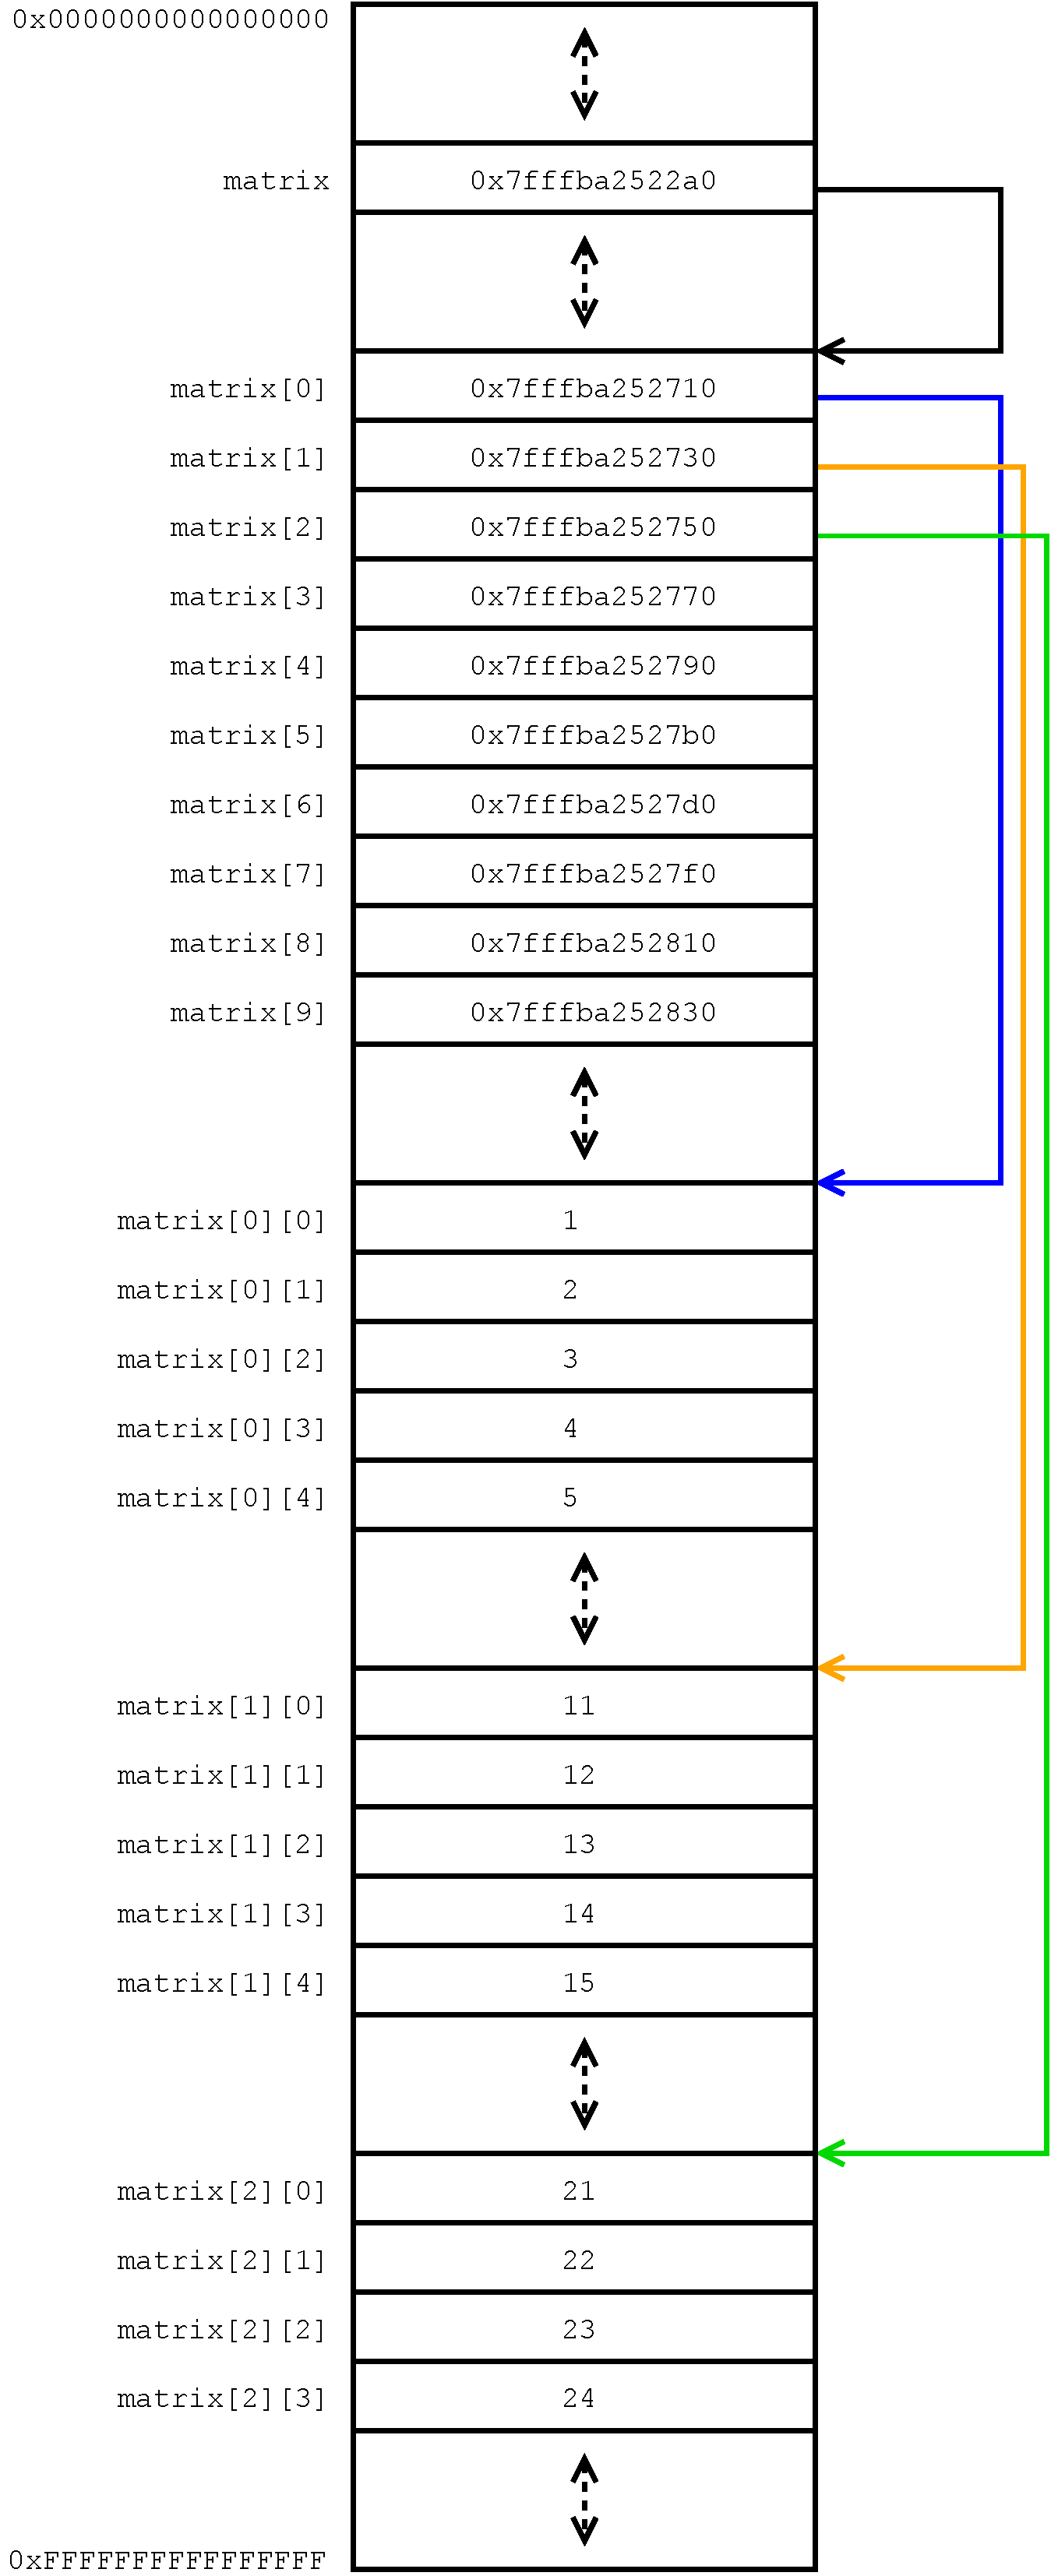
\includegraphics[height=225mm]{double_pointer_map}
    \caption{Mapa de memoria de un vector de vectores (doble puntero)}
    \label{img:double_pointer_map}
\end{figure}

En la figura represento el mapa de memoria, a la izquierda están los nombres
que tienen esas ubicaciones de memoria en el programa, y en el rectángulo
expreso su contenido. Las flechas del lado derecho de la imagen representan las
referencias de los punteros a dichas direcciones de memoria. Los colores
simplemente sirven para que puedas seguirlas más fácilmente. Bien, si miras
donde pongo la etiqueta \verb!matrix!, verás que contiene una dirección de
memoria, esta dirección referencia a un \textbf{vector de punteros}, es decir,
\verb!rows! punteros juntos. Cada uno de estos punteros apunta, a su vez, a una
región
contigua de memoria, en la cual se guarda una fila entera de la matriz. Sólo
he representado las primeras tres filas, porque si no la figura sería excesivamente
grande.

Ahora voy a poner la figura de cómo sería el mapa de memoria en el caso de un
array doble, no incluyo el código porque su declaración sería simplemente
\lstinline[style=C]!int matrix[10][5]!.

\begin{figure}[H]
    % Lo centramos
    \center
    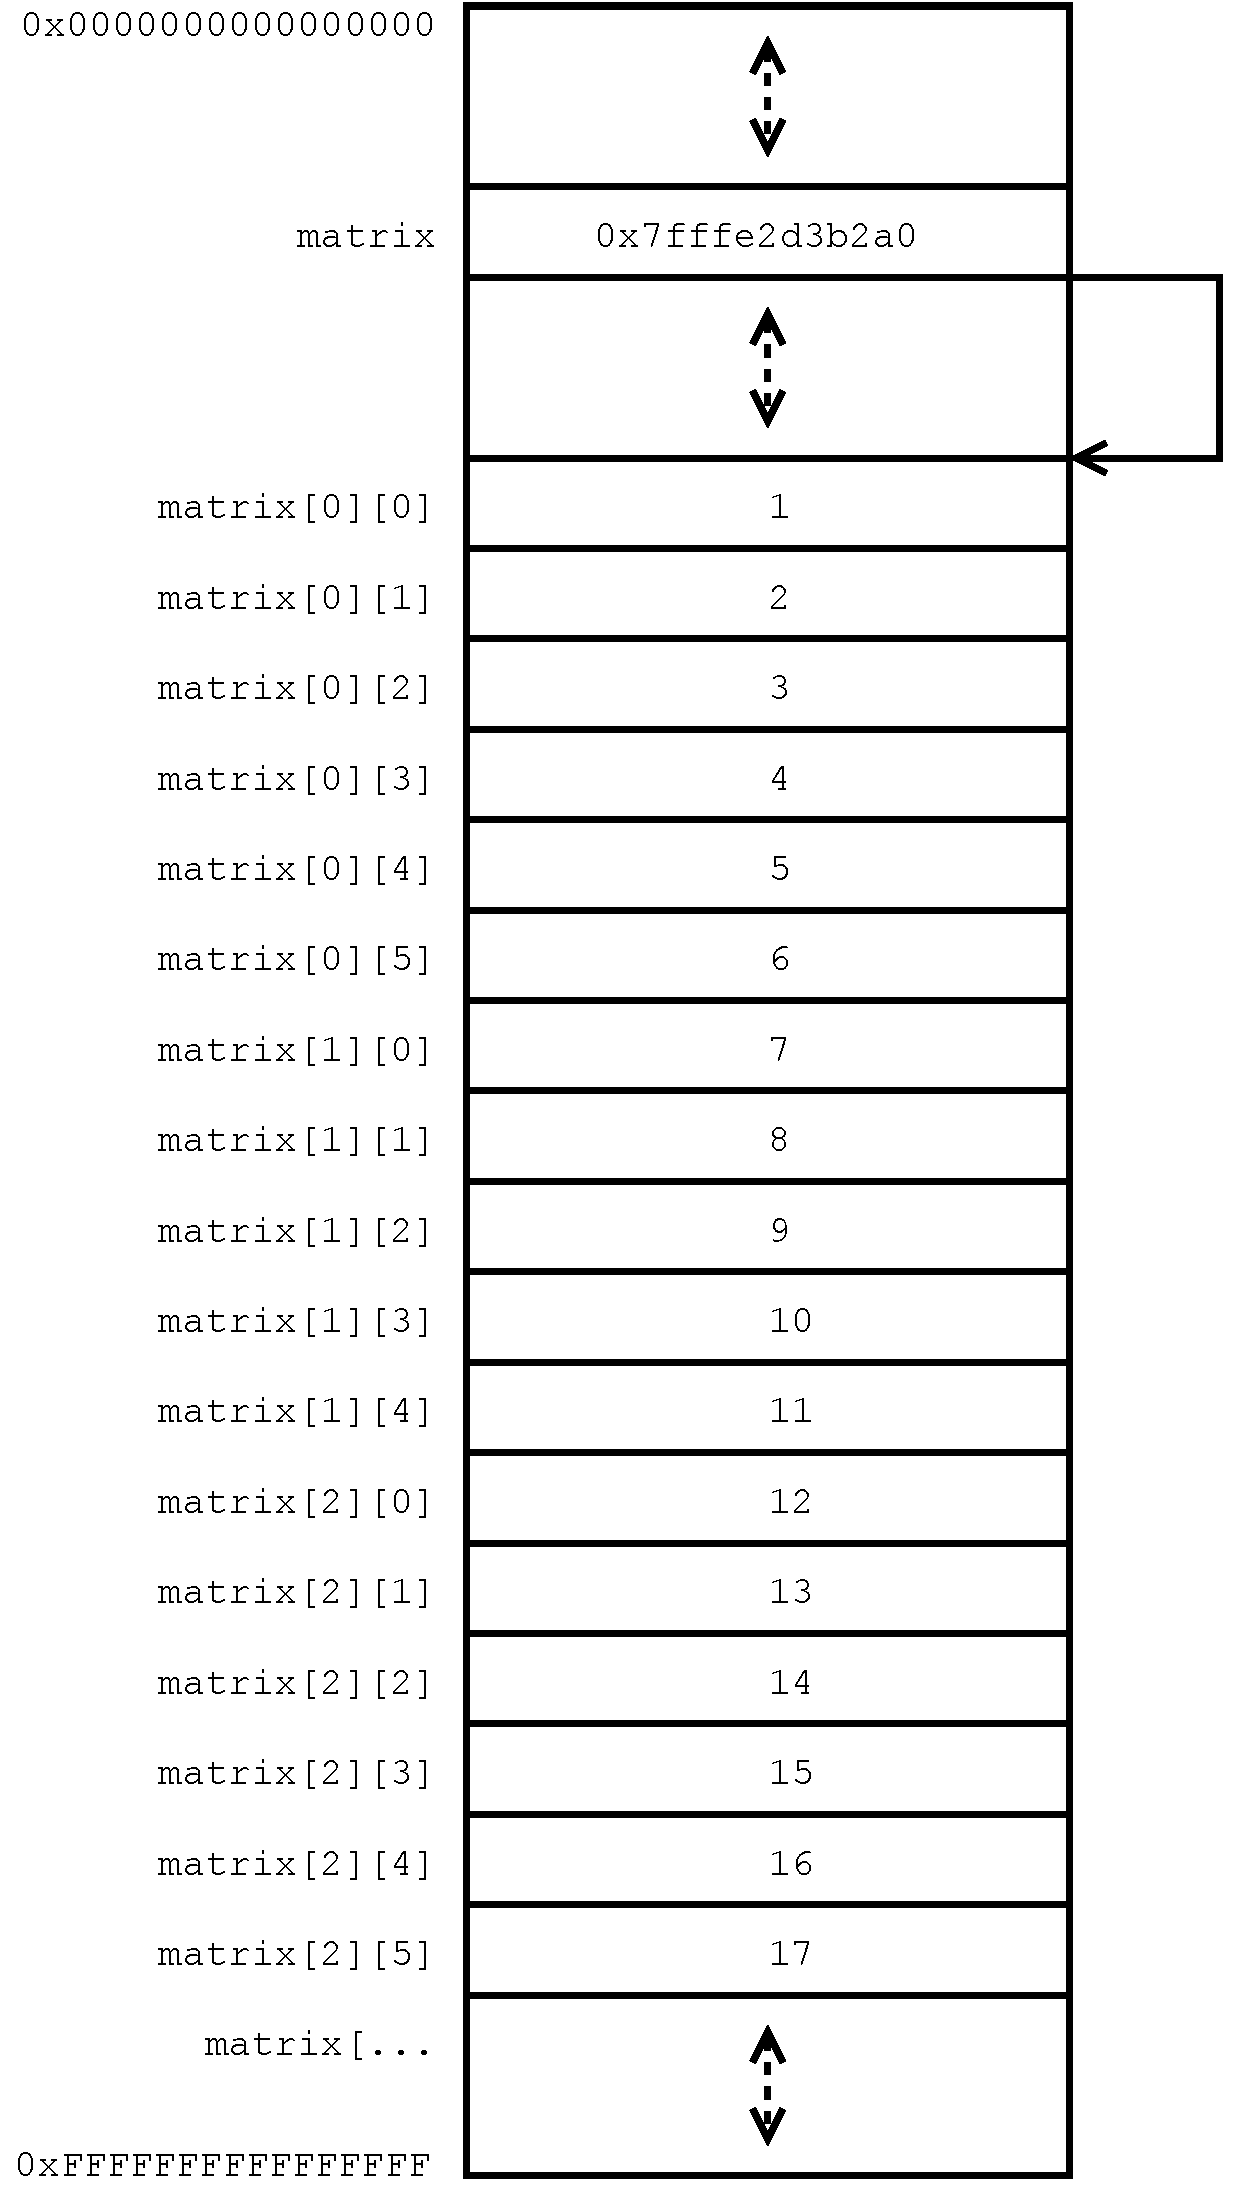
\includegraphics[width=.5\linewidth]{double_array_map}
    \caption{Mapa de memoria de un doble array}
    \label{img:double_array_map}
\end{figure}

Como puedes ver, aunque el array es de dos dimensiones, no hay una segunda
desreferenciación. Es decir, en ningún momento se sigue un segundo puntero.
¿Cómo es esto posible? Si miras el mapa, verás que el array se almacena en
una región de memoria continua. Esto quiere decir que C sólo tiene que
adquirir la dirección de inicio del array y, después, sumarle lo que indiquen
los operadores corchete. Es aquí donde se presenta un problema cuando intentamos
pasar un array bidimensional a una función. Llegados a la función, C no sabe
si ese puntero que tiene es un vector de vectores o un array de arrays, por
ello, si le pasaras este array doble a una función que recibe un puntero doble,
al hacer, por ejemplo, \verb!matrix[1][2]! lo que intentaría hacer es acceder
como si fuera un puntero, y haría: \verb!*((*(matrix + 1))+2)! Es decir, primero
sumaría (recuerda la aritmética de punteros) uno a la dirección base, después,
\textbf{interpretaría su contenido como un puntero} a otro vector, y a ese
intentaría sumarle 2 para desreferenciarlo. El problema es que
\verb!*(matrix+1)! \textbf{no es} un puntero, es directamente el número.

C puede hacer esto porque, del mismo modo que te indiqué cuando te expliqué
cómo funciona el operador \verb!sizeof!, podemos ver que C sabe el tamaño de un
array siempre que éste no decaiga a puntero, es decir, puedes saber el tamaño
de un array en cualquier alcance interior a aquél en que fue declarado.

La conclusión lógica de lo que acabamos de ver es que el número máximo de
dimensiones de array que puede recibir cualquier función es uno, porque es el que
se comporta como un puntero sin problemas. El hecho de que el array, por ser
declarado en una única orden, sea una estructura continua en memoria hace que
pueda ser interpretado como una estructura de una sola dimensión. Por ejemplo,
en el siguiente código declaramos y rellenamos un array de dos dimensiones y,
sin embargo, podemos acceder a él como si sólo tuviera una dimensión.

\noindent
\begin{minipage}[H]{\linewidth}
\mbox{}
\begin{lstlisting}[style=C,
caption={Uso de un array como una estructura unidimensional},
label={lst:bidimensionalArrayAsOneDimension}]
#include <stdio.h>
#include <stdlib.h>

int main(void)
{
    int rows = 10;
    int columns = 5;
    int matrix[10][5];

    printf("matrix = %p\n", matrix);

    for (int ii = 0; ii < rows; ++ii) {
        for (int jj = 0; jj < columns; ++jj) {
            matrix[ii][jj] = ii * columns + jj + 1;
        }
    }

    for (int ii = 0; ii < rows * columns; ++ii) {
        printf("%d\n", (*matrix)[ii]);
    }

}
\end{lstlisting}
\end{minipage}

Como puedes ver, una vez hemos llegado a la región contigua de memoria, es decir
\verb!(*matrix)!, sólo tenemos que recorrerla como si fuera un array
unidimensional.

\subsection{Ejercicios de la sección}
\begin{exercises}[resume*]
\item Completa esta tabla de números en diferentes bases numéricas:
\begin{table}[H]
\begin{tabularx}{\linewidth}{|R|R|R|}
\hline
\multicolumn{1}{|Y|}{\textbf{Decimal}}& \multicolumn{1}{Y|}{\textbf{Binario}} & \multicolumn{1}{Y|}{\textbf{Hexadecimal}} \\\hline
73&  &  \\\hline
   &00100110& \\\hline
&&0x12F       \\\hline
128&&         \\\hline
\end{tabularx}
\end{table}
\item Vuelve al ejercicio noveno y reproduce los contenidos de la pila en cada
bloque de código del programa. Utiliza de referencia la solución que propongo
yo.
\item Haz un programa que cree un puntero de tres niveles de tipo \verb!int!,
lo reserve correctamente, lo rellene con el valores correlativos
\textbf{empezando en uno} y después lo imprima de una manera comprensible.
Finalmente, libéralo también de tal modo que no quede memoria sin liberar al
final del programa.
\item Basándote en el programa anterior, crea dos funciones, una para crear
una matriz tridimensional con memoria dinámica dadas sus tres dimensiones y
otra para liberarla.
\end{exercises}
\section{Modificadores de tipos: constancia y signo}
\label{sec:typeModifications}

Hasta ahora sólo hemos manejado los tipos básicos, pero a esos tipos se les
pueden añadir \textbf{modificadores}, que son cualidades que crean un tipo
ligeramente distinto basado en el anterior. El primero y más importante es el
modificador \lstinline[style=C]!const!. Éste nos permite indicar que una
variable es \textbf{de sólo lectura}, es decir, que una vez le demos valor
cuando la declaramos, no podremos modificarla. Esto es muy útil para asegurarnos
de que no introducimos errores en el código cuando manejamos datos que no deben
ser cambiados.

Por ejemplo, imagínate un programa que utilice el número $\pi$. Por ejemplo
para calcular el área de un círculo, necesitaríamos escribir
\verb!surface = PI * pow(r, 2)!. Pero, imagina que nos equivocamos y escribimos
\verb!surface = PI *= pow(r, 2)!, este error sería muy difícil de ver porque
la primera vez la superficie estaría bien calculada, pero \verb!PI! habría
quedado sobreescrita por el uso del operador \verb!*=!, y todos los cálculos
posteriores serían incorrectos. Si declaramos \verb!PI! como una constante,
el compilador nos notificará de estos errores.

\noindent
\begin{minipage}[H]{\linewidth}
\mbox{}
\begin{lstlisting}[style=C,
caption={Uso de una constante numérica},
label={lst:constantUsage}]
#include <stdio.h>
#include <stdlib.h>

const double PI = 3.141592;

double surface_circle(double radius) {
    return PI * radius * radius;
}

double perimeter(double radius) {
    return 2 * PI * radius;
}

int main(void)
{
    double r = 3.5;
    printf("Un círculo con un radio de %.3f tiene un perímetro de %.2f y un área de %.2f\n", r, perimeter(r), surface_circle(r));
}
\end{lstlisting}
\end{minipage}

En la línea cuatro del código puedes ver cómo declaramos \verb!PI! como una
constante de tipo \verb!double!. Puedes ver que, además, estamos declarándola
como variable global. Si recuerdas cuando te expliqué el alcance las variables y
lo que era una variable global, te dije que era útil cuando había funciones.
Aquí puedes ver uno de los usos comunes de las variables globales, cuando se
definen constantes universales, como podrían ser $\pi$, $e$ o la constante
gravitatoria $G$. Pero volviendo al hecho de la constante, si intentas escribir
una instrucción que modifique la constante, el compilador lanzará un error como
este:

\noindent
\begin{minipage}[H]{\linewidth}
\mbox{}
\begin{lstlisting}[style=terminalStyle]
\$  gcc -o main.exe main.c
main.c: In function 'main':
main.c:17:8: error: assignment of read-only variable 'PI'
   17 |     PI = 1.1;
      |        ^
\end{lstlisting}
\end{minipage}

Pero el modificador \verb!const! se aplica en otro sitio muy importante,
se utiliza en las declaraciones de los argumentos de las funciones para indicar
que los argumentos no se pueden modificar. De nuevo, los argumentos de las
funciones son copias de sus valores, así que, sabiendo esto, no tendría utilidad
una manera de decir que no los podemos modificar, el asunto nuclear de esto es
que el modificador \verb!const! se aplica a punteros, indicando que no se puede
modificar su contenido, y es ahí donde se vuelve tremendamente útil en
conjunción con las funciones. Por ejemplo, volvamos a la función que utiliza
punteros para calcular la distancia entre dos estructuras \verb!point_s!, como
no queremos que estas estructuras sean modificadas por la función, we can do
this:

\noindent
\begin{minipage}[H]{\linewidth}
\mbox{}
\begin{lstlisting}[style=C,
caption={Uso de punteros constantes como argumentos de función},
label={lst:constantArguments}]
#include <stdio.h>
#include <stdlib.h>
#include <math.h>

struct point_s {
    double x; double y;
};

double distance(const struct point_s* a, const struct point_s* b) {
    double res = 0.0;
    struct point_s origin = { .x = 0.0 , .y = 0.0 };
    if (NULL == a) {
        a = &origin;
    }
    if (NULL == b) {
        b = &origin;
    }
    double diff_x = a->x - b->x;
    double diff_y = a->y - b->y;
    res = sqrt(diff_x * diff_x + diff_y * diff_y);
    return res;
}

int main(void)
{
    struct point_s a = { .x = 3 , .y = 4 };
    double d = distance(&a, NULL);
    printf(" Distance : %f\n", d);

}
\end{lstlisting}
\end{minipage}

Si miras el programa, la única diferencia es que en la declaración anteponemos
el modificador \verb!const! delante del tipo del dato. Esto impide que
modifiquemos el contenido de este puntero dentro de la función. Si intentas
hacer, por ejemplo: \verb!a->x++;! el compilador lanzará un error. Esto es de
suma utilidad para el programador que use la función sin haberla escrito,
porque así entiende si una función va a modificar los datos que éste le pase,
sin necesidad de saber qué hacer la función por dentro. Cuando veamos cómo
dividir el programa en varios archivos, verás la importancia de esto en su
totalidad.

Además, el modificador \verb!const! añade el concepto de
\textit{const correctness}, este concepto es aquél por el cual hay que respetar
la cualidad de constancia de las variables y argumentos. Esto quiere decir que
debes definir tus funciones con cuidado de indicar todo lo que sea posible
como constante. Por ejemplo, en el caso de la función que calcula la distancia
entre dos puntos los dos argumentos deben ser constantes. Pero es más, una
función \textbf{puede devolver una constante}. Esto sirve cuando se crean
estructuras de datos que no quieres que el usuario sea capaz de modificar
directamente, sino sólo mediante las funciones que tú quieras.

Hablaremos más de esto en un futuro, pero te pongo un ejemplo básico:
imagínate una estructura que guarda datos de una persona.
En esta estructura
tendremos varios punteros a \verb!char!: el nombre, un primer apellido y un
segundo apellido. Lo que haremos es crear una función que cree esta estructura
recibiendo los tres textos, reservará la memoria necesaria y después copiará
los textos a esa memoria. Después, para manejar esa estructuras vamos a crear
funciones que reemplacen estos arrays cuando el usuario quiera. Vamos a por
ello:

\noindent
\begin{minipage}[H]{\linewidth}
\mbox{}
\begin{lstlisting}[style=C,
caption={Estructura con punteros constantes -- Funciones de manipulación},
label={lst:structConstPointers}]
#include <stdio.h>
#include <stdlib.h>
#include <string.h>

struct person_s {
    char* name;
    char* last_name_1;
    char* last_name_2;
};

struct person_s person_create(const char* name,
                              const char* last_name_1,
                              const char* last_name_2) {
    struct person_s res;

    res.name        = malloc(strlen(name) + 1);
    res.last_name_1 = malloc(strlen(last_name_1) + 1);

    for (int ii = 0; ii < strlen(name) + 1; ++ii) {
        res.name[ii] = name[ii];
    }

    for (int ii = 0; ii < strlen(last_name_1) + 1; ++ii) {
        res.last_name_1[ii] = last_name_1[ii];
    }

    if (NULL != last_name_2) {
        res.last_name_2 = malloc(strlen(last_name_2) + 1);
        for (int ii = 0; ii < strlen(last_name_2) + 1; ++ii) {
            res.last_name_2[ii] = last_name_2[ii];
        }
    }
    else {
        res.last_name_2 = NULL;
    }
    return res;
}

void person_set_name(struct person_s* person, const char* name){
    free(person->name);
    person->name = malloc(strlen(name)+1);
    for(int ii = 0; ii < strlen(name) + 1; ++ii){
        person->name[ii] = name[ii];
    }

}

void destroy_person(struct person_s *person){
    free(person->name);
    free(person->last_name_1);
    free(person->last_name_2);
}
\end{lstlisting}
\end{minipage}

\noindent
\begin{minipage}[H]{\linewidth}
\mbox{}
\begin{lstlisting}[style=C,
caption={Estructura con punteros constantes -- Funciones de recuperación de información},
label={lst:structConstGetters}]
const char* person_get_name(const struct person_s* person) {
    return person->name;
}

const char* person_get_last_name_1(const struct person_s* person) {
    return person->last_name_1;
}

const char* person_get_last_name_2(const struct person_s* person) {
    if (NULL == person->last_name_2) {
        return "";
    }
    else {
        return person->last_name_2;
    }
}

\end{lstlisting}
\end{minipage}

\noindent
\begin{minipage}[H]{\linewidth}
\mbox{}
\begin{lstlisting}[style=C,
caption={Estructura con punteros constantes -- función \texttt{main}},
label={lst:structConstMain}]
int main(void)
{
    struct person_s myself = person_create("Francisco", "Rodríguez", "Melgar");

    printf("Esta persona es: %s %s %s\n", person_get_name(&myself),
            person_get_last_name_1(&myself),
            person_get_last_name_2(&myself));

    person_set_name(&myself, "José");

    printf("Esta persona es: %s %s %s\n", person_get_name(&myself),
           person_get_last_name_1(&myself),
           person_get_last_name_2(&myself));

    destroy_person(&myself);
}
\end{lstlisting}
\end{minipage}
En este código puedes ver como <<ocultamos>> al usuario cómo manejamos estos
punteros. Para impedir que él cambie su contenido sin utilizar nuestras
funciones, las funciones que devuelven los punteros para poder usarlos, por
ejemplo para imprimirlos, devuelven punteros constantes. Si intentaras hacer,
por ejemplo: \lstinline[style=C]!person_get_name(&myself)[3] = 'a'! el
compilador lanzaría un error. Esto es una herramienta para impedir que el
usuario de la estructura se olvide de liberar la memoria a la hora de reemplazar
el texto por otro.

Si estás atento, te habrás dado cuenta de que todo esto es algo inútil cuando
el usuario de la estructura podría simplemente escribir
\verb!myself.name[0] = 'a'!, y tendrías razón. En secciones posteriores veremos
maneras de evitar esto. Pero incluso con este problema, hacer esto es una buena
manera de ahorrarle trabajo al usuario de la estructura.

El otro modificador que quiero presentarte es el signo, o mejor dicho, la
ausencia de signo. La palabra reservada \lstinline[style=C]!unsigned! nos
permite declarar variables de los mismos tipos que los tipos básicos, pero
que sólo contengan valores positivos. Si no ves a primera vista la utilidad de
esto, ésta reside en que al hacer el tipo sin signo, aumentas el rango que puede
almacenar en los números positivos, si un \verb!char! tiene un rango en
$[-127, 128]$, al hacerlo sin signo, éste tiene un rango de $[0, 255]$. Además,
esto permite añadirle significado a tus variables.

Por ejemplo, una variable que guarde el tamaño de algo, por ejemplo de un array
o de un vector, no debería tener signo, porque nunca puede ser negativa. Una
variable que guarde un mes, por ejemplo, tampoco. En el caso de tamaños de
arrays o vectores es importante porque hacer las variables que guardan su
tamaño no tengan signo, porque así nos permite hacer arrays el doble de grandes.
No existen tipos sin signo para números de coma flotante (\verb!float!
y \verb!double!).
Veamos un ejemplo de cómo utilizar el modificador \verb!unsigned! para declarar
variables, argumentos y tipos de retorno.

\noindent
\begin{minipage}[H]{\linewidth}
\mbox{}
\begin{lstlisting}[style=C,
caption={Uso de tipos sin signo},
label={lst:unsignedTypes}]
#include <stdio.h>

unsigned int factorial(unsigned int n) {
    unsigned int res = 1;
    for (unsigned int ii = 0; ii < n; ++ii) {
        res *= n - ii;
    }
    return res;
}

int main(void)
{
    unsigned int number = 10;
    printf("%d! =%d\n", number, factorial(number));
}
\end{lstlisting}
\end{minipage}

Sé que parece un poco engorroso escribir \verb!unsigned! cada vez, más adelante
veremos cómo solventar esto.
\subsection{Ejercicios de la sección}
El ejercicio más apropiado es que revises todos los ejercicios que
hemos hecho hasta ahora y los reescribas teniendo en cuenta la constancia de las
funciones y el signo.
\section{Comunicar tu programa con el exterior}
Por fin vamos a llegar al punto en que tu programa pueda comunicarse con el
exterior, hasta ahora, todos los datos que hemos introducido en el programa
están escritos en el código como literales. Eso es muy impráctico, en términos
generales, un programa leerá, ya sea por consola o desde un archivo concreto,
los datos que deba utilizar. Hay tres fuentes de información externa
básicas que vamos a manejar:
\begin{enumerate}
\item Argumentos de la línea de comandos.
\item La entrada por consola.
\item Ficheros.
\end{enumerate}

Lo primero es algo que aún no sabes qué es, pero que será bastante útil. Hasta
ahora, la función \verb!main! no recibía ningún argumento, pero puede
recibirlos. Si \verb!main! es una función que sólo sirve como punto de entrada
a nuestro programa, ¿quién la puede llamar con argumentos? Básicamente
estos argumentos vienen de la línea de comandos con la que llamemos a nuestro
programa. Para poder acceder a ellos dentro del programa, debemos declarar
la función \verb!main! de este modo:

\noindent
\begin{minipage}[H]{\linewidth}
\mbox{}
\begin{lstlisting}[style=C,
caption={Declaración de una función \texttt{main} que reciba argumentos},
label={lst:mainArguments}]
int main(int argc, const char** argv) {
// ...
\end{lstlisting}
\end{minipage}

De estos dos argumentos, el primero es el número de argumentos que ha recibido
tu programa, y el segundo es un vector de vectores a \verb!char! que nos llega
en forma de puntero a puntero. Los argumentos que recibe un programa vienen
en formato de cadenas de texto, por lo que, si son números, debemos utilizar
funciones auxiliares para convertirlos a esos tipos de dato. Vamos a hacer
un programa que reciba un número indeterminado de argumentos y los imprima, cada
uno en una línea nueva.

\noindent
\begin{minipage}[H]{\linewidth}
\mbox{}
\begin{lstlisting}[style=C,
caption={Utilización de los argumentos de un programa},
label={lst:argumentProgram}]
#include <stdio.h>

int main(int argc, char const *argv[])
{
    for (int ii = 0; ii < argc; ++ii) {
        printf("%s\n", argv[ii]);
    }
}
\end{lstlisting}
\end{minipage}

Y quizás te preguntes que cómo le paso esos argumentos al programa, bien, es
sencillo: al llamar el programa, después de la ruta al ejecutable, pones
todos los argumentos separados por espacios, por ejemplo:
\begin{lstlisting}[style=terminalStyle]
\$./main.exe argumento1 argumento2 argumento3
\end{lstlisting}
Si compilas este programa y lo ejecutas con esos argumentos, imprimirá esto:

\begin{lstlisting}[style=terminalStyle]
./main.exe
argumento1
argumento2
argumento3
\end{lstlisting}

Y sí, como ves, el primer argumento es el comando con el que se llamó el
programa, esto es importante porque, como deducirás, quiere decir que tu
programa siempre recibirá al menos uno. Este primer argumento cambia según la
orden con la que llamemos a nuestro programa, por ejemplo, si en vez de con
esa ruta relativa lo llamamos con una ruta absoluta, obtendríamos los siguiente:
\begin{lstlisting}[style=terminalStyle]
\$ /home/usuario/test/project/main.exe arg1 arg2 arg3
/home/usuario/test/project/main.exe
arg1
arg2
arg3
\end{lstlisting}

Como última nota, si el espacio es el carácter que se usa para separar
argumentos, ¿pueden tener espacios los argumentos? Sí, simplemente rodea el
argumento de comillas dobles. Y, entonces, ¿pueden tener comillas dobles? Sí,
simplemente pon una barra inversa delante de la comilla, veamos un ejemplo
rápido,
\begin{lstlisting}[style=terminalStyle]
\$ ./main.exe "Esto es una comilla: \"" \"\"\" "Frase con espacios"
./main.exe
Esto es una comilla: "
"""
Frase con espacios
\end{lstlisting}

Si necesitamos leer un número, debemos utilizar, como ya hemos dicho, una
función que nos convierta el argumento en un número. La función básica para
hacer esto es \verb!atoi! (del inglés: \emph{ASCII to integer}). Por ejemplo,
vamos a crear un programa que reciba una serie de argumentos y los sume:

\noindent
\begin{minipage}[H]{\linewidth}
\mbox{}
\begin{lstlisting}[style=C,
caption={Programa que suma argumentos},
label={lst:sumArgs}]
#include <stdio.h>
#include <stdlib.h>

int main(int argc, char const* argv[])
{

    int total = 0;

    for (int ii = 1; ii < argc; ++ii) {
        total += atoi(argv[ii]);
    }

    printf("La suma de los argumentos es: %d\n", total);
}
\end{lstlisting}
\end{minipage}

Nota que empezamos a sumar desde el segundo argumento (la posición uno del
vector) porque el primero no es un número. Esto me lleva a advertirte de que
\verb!atoi! es una función muy básica y si introduces en ella una cadena que no
es un número, devolverá valores sin sentido, en muchas ocasiones 0. Así
que ten cuidado sobre esto. De todos modos, en otras secciones veremos maneras
de manipular cadenas de texto más complejas que nos permitirán comprobarlo.
Sería un ejercicio interesante que hicieras un programa que comprobara si una
cadena de texto es un número o no. Finalmente, también existe \verb!atof! que
hace lo mismo, pero con decimales.

Otra opción que existe que dejar que, una vez iniciado el programa, el usuario
escriba por consola lo que deba éste recibir. Por ejemplo, podríamos hacer un
programa que sea una versión 2.0 de nuestro primer \emph{Hola Mundo}. Esta
versión podría primero preguntar el nombre del usuario y después saludarle por
él. Para conseguir esto se utiliza (o se puede utilizar, hay otras alternativas)
la función \verb!scanf!. Esta función es la hermana gemela de \verb!printf!
porque se comporta igual, simplemente especificas un formato y le das las
variables donde quieres guardar los datos y la función leerá de la terminal
con ese formato. Por ejemplo, hagamos este \emph{Hola Mundo 2.0}.

\noindent
\begin{minipage}[H]{\linewidth}
\mbox{}
\begin{lstlisting}[style=C,
caption={Ejemplo básico de \texttt{scanf}},
label={lst:basicScanf}]
#include <stdio.h>
#include <stdlib.h>

#define NAME_LENGTH ((size_t)1024)

int main(int argc, char const* argv[])
{

    char name[NAME_LENGTH] = "";
    printf("Hola, ¿cuál es tu nombre?\n");
    scanf("%s", name);
    printf("Escantado de conocerte, %s.\n", name);
}
\end{lstlisting}
\end{minipage}

Como puedes ver, es sencillo, pero debes tener en cuenta que si lees tipos
de datos básicos con \verb!scanf! debes pasarle punteros a esas variables. En
el caso de un puntero a \verb!char! es menos evidente. Además, salvo que llames
a otras funciones para cambiar cómo se comporta la terminal, \verb!scanf! sólo
leerá hasta el primer carácter en blanco que se encuentre, es decir, hasta el
primer espacio, por ejemplo. Eso quiere decir que si quieres leer varias
palabras debes invocar a \verb!scanf! varias veces o invocarlo con varios
especificadores de formato. Vamos a ver un ejemplo un poco más complicado para
que quede todo esto claro.

\noindent
\begin{minipage}[H]{\linewidth}
\mbox{}
\begin{lstlisting}[style=C,
caption={Ejemplo avanzado de \texttt{scanf}},
label={lst:scanfExample}]
#include <stdio.h>
#include <stdlib.h>

#define NAME_LENGTH ((size_t)1024)

int main(int argc, char const* argv[])
{

    char name[NAME_LENGTH] = "";
    int age = 0;
    double height = 0.0;
    printf("Hola, quiero conocerte, dime tu nombre, tu edad y cuánto mides en metros\n");
    scanf("%s %d %lf", name, &age, &height);
    printf("Encantado de conocerte, %s. Así que tienes %d años y mides %f m\n", name, age, height);
}
\end{lstlisting}
\end{minipage}

Como hemos dicho, \verb!scanf! deja de leer en los espacios, así que puedes
escribir cada dato y pulsar enter o escribir las tres respuestas separadas
por espacios y darle a enter una sola vez. Además, nota que, como queremos
leer en un \verb!double!, tenemos que usar el especificador \verb!%lf!,
el compilador lanza un \emph{warning} si lo dejamos con simplemente \verb!%f!.
Esta función
\textbf{bloquea} el programa hasta que recibe \textbf{todos} los argumentos
pedidos por los especificadores. Además, lo que se escriba en la terminal y
no se consuma (se lea por \verb!scanf!) queda pendiente para llamadas
posteriores, es decir, si en vez de escribir en nuestro ejemplo una sola
llamada, escribieras tres, una con cada especificador y variable, el efecto
sería el mismo, podrías seguir escribiendo todo separado por espacios. Del
mismo modo que \verb!atoi!, si especificas que recibirá números y la entrada
es distinta, fallará dando valores con poco o ningún sentido.

Y finalmente: los ficheros, o archivos. Los programas pueden eliminar, crear,
escribir y leer de archivos. Para esto hay varias maneras, algunas más pedestres
que otras, porque algunas son más estándar y otras dependen del sistema
operativo. Al contrario que con los otros métodos, los ficheros tienen un
ciclo de vida más complejo. El ciclo de vida es, en este contexto, la descripción
de cuándo empieza a existir, existe y deja de existir algo. Por ejemplo,
el ciclo de vida de una región de memoria dinámica es desde que la reservas
hasta que la liberas, el de un array, desde que se entra en su bloque de código
hasta que se sale, etc. Con los archivos pasa algo parecido.

Los archivos son un concepto que, de nuevo, gestiona el sistema operativo,
de tal modo que tenemos que utilizar funciones concretas para abrirlos, escribir
y leer en ellos y, finalmente, cerrarlos. A la mínima que estés un poco atento,
verás el paralelismo entre esto y la reserva de memoria. La función para abrir
un archivo es \lstinline[style=C]!fopen!, veamos su declaración:

\noindent
\begin{minipage}[H]{\linewidth}
\mbox{}
\begin{lstlisting}[style=C,
caption={Declaración de la función \texttt{fopen}},
label={lst:callocSignature}]
FILE *fopen(const char *pathname, const char *mode);
\end{lstlisting}
\end{minipage}

Devuelve un puntero a un tipo llamado \verb!FILE!, este tipo es \textbf{opaco},
esta es una palabra que se utiliza en informática para decir que no puedes saber
lo que hay dentro, es decir, es el sistema quien lo gestiona y tú sólo
interactúas con este tipo mediante llamadas a función. Los argumentos de esta
función son dos punteros a \verb!char!. El primero es la ruta al archivo.
Esta ruta puede ser relativa o absoluta, pero ten cuidado, si es relativa, ésta
toma como origen \textbf{el directorio de trabajo} de la terminal donde lo
ejecutes. Es decir, si le dices a la función que abra un archivo en la ruta
\verb!./file.txt!, lo buscará (o lo creará, según proceda), en tu directorio
de trabajo, no en el que se encuentre el ejecutable, salvo que sean el mismo.

El segundo argumento es interesante, es, como indica su nombre, el modo de
apertura del archivo. En éste argumento se suele escribir un literal que
contiene una serie de letras, estas letras son atributos a la manera en que
abrimos el archivo, veamos qué opciones tenemos.
\begin{enumerate}
\item \verb!r!: Abre el archivo para lectura (sólo para lectura) la cabeza
de lectura se sitúa al inicio del archivo. Si el archivo no existe, se produce
un error y la función devuelve \verb!NULL!.
\item \verb!r+!: Igual que la anterior, pero permite escribir también.
\item \verb!w!: \textbf{Vacía} el archivo o lo crea si no existe
y permite escribir en él, situando la cabeza de lectura, lógicamente, al inicio.
\item \verb!w+!: Igual que la anterior, pero permite leer también.
\item \verb!a!: Abre el archivo para escribir, pero \textbf{no lo vacía},
sí que lo crea si no existe. La cabeza se sitúa al final del archivo, para
\textbf{añadir} a al contenido que hubiera.
\item \verb!a+!: El archivo es creado si no existe, se escribirá al final
del mismo y permite también leer.
\end{enumerate}

En la descripción de las opciones hablo de una cosa llamada cabeza de lectura.
Es un concepto propio de los ficheros, en un fichero el programa guarda la
posición del mismo en el que está esta cabeza. Cuando escribes o lees, ésta
se mueve hacia delante tanto como el tamaño de los datos que hayas leído o
escrito.
Una analogía que se solía utilizar es que un fichero es como una cinta de vídeo,
y el cabezal de lectura como el del reproductor. El cabezal empieza al inicio
de una cinta, supongamos que ves 10 minutos, la pausas y la vuelves a reaundar,
empezarás
desde donde lo dejaste. Puedes rebobinar, avanzar el vídeo y, además, ver partes
del vídeo hace que la cabeza avance. Es decir, leer avanza el cabezal, y si
quieres ver algo qhe ya viste debes rebobinar.
Todo sea dicho, el cabezal de lectura es único por
proceso y archivo, así que dos programas pueden leer o escribir en el mismo
archivo en puntos distintos. Por otro lado, cuando la cabeza de lectura llega
al final, se para allí (lógicamente), pero si estás realizando una operación
de escritura, el archivo se agrandará, como es lógico, porque de no ser así,
no podríamos escribiríamos en archivos nuevos o vacíos.

Ahora que ya sabes cómo abrir un archivo, veamos cómo se lee o escribe de él.
Las funciones que se usan para esto son dos: \verb!fwrite! y \verb!fread!.

\noindent
\begin{minipage}[H]{\linewidth}
\mbox{}
\begin{lstlisting}[style=C,
caption={Declaración de la función \texttt{fread}},
label={lst:freadSignature}]
size_t fread(void *ptr, size_t size, size_t nmemb, FILE *stream);
\end{lstlisting}
\end{minipage}

\noindent
\begin{minipage}[H]{\linewidth}
\mbox{}
\begin{lstlisting}[style=C,
caption={Declaración de la función \texttt{fwrite}},
label={lst:fwriteSignature}]
size_t fwrite(const void *pt, size_t size, size_t nmemb, FILE *stream);
\end{lstlisting}
\end{minipage}

Las dos funciones se comportan más o menos igual, reciben un puntero, un tamaño,
otro número y finalmente el puntero a la estructura que simboliza el fichero.
El primer puntero es de entrada para escribir y de salida para leer. Es donde
pondremos nuestros datos, o la memoria para que la función lo escriba cuando
leemos. Es un puntero a \verb!char!, que es el puntero que se utiliza para
simbolizar una continuidad de datos genérico, es decir, un continuo de bytes.
Estas funciones están hechas para escribir o leer objetos de un determinado
tamaño, de ahí que existan los argumentos \verb!size! y \verb!nmemb!; el primero
es el tamaño de cada uno de los objetos y el segundo el número de ellos que
queremos leer o escribir. La función devuelve el número de \textbf{objetos}
escritos o leídos, no de bytes. Más sobre esto en los ejemplos.

Finalmente, después de hacer lo que deseas con los archivos que has abierto,
debes cerrarlo. Cerrar el archivo provoca que todos los cambios que se han
escrito se sincronicen con el disco duro o sistema de almacenamiento subyacente.
Esto es importante, si te olvidas de cerrar un archivo puedes ver que cambios
que has escrito no se reflejan en el archivo. La función para cerrar archivos
se llama \verb!fclose!, su \emph{signature} es la siguiente.

\noindent
\begin{minipage}[H]{\linewidth}
\mbox{}
\begin{lstlisting}[style=C,
caption={Declaración de la función \texttt{fclose}},
label={lst:fcloseSignature}]
int fclose(FILE *stream);
\end{lstlisting}
\end{minipage}
Como puedes ver, sólo recibe el archivo que deseamos cerrar o liberar.

Ahora que ya hemos explicado las funciones que hay que utilizar, vamos a ver
un ejemplo simple de programa que utilice ficheros. Un programa muy típico
podría ser uno que copie un fichero a otro, como el comando \verb!cp!, que es
el que se usa en Linux para hacer eso. Vamos a hacer un programa que reciba dos
argumentos, el primero será el archivo que deseamos copiar y el segundo dónde.
El comando en Linux admite que la segunda localización sea una carpeta, es
decir, podrías hacer \verb!cp ~/novel.txt /home/joe/novels! pero para hacer
más sencillo nuestro ejemplo, obligaremos a que el usuario siempre especifique
dos rutas completas. Veamos cómo se haría.

\noindent
\begin{minipage}[H]{\linewidth}
\mbox{}
\begin{lstlisting}[style=C,
caption={Ejemplo de manejos de ficheros},
label={lst:fileBasic}]
#include <stdio.h>
#include <stdlib.h>

int main(int argc, char const* argv[])
{

    FILE *origin_file  = NULL;
    FILE *destiny_file = NULL;
    char byte          = 0;

    if (argc < 3) {
        printf("Uso: main.exe <origen> <destino>\n");
        return EXIT_FAILURE;
    }

    origin_file = fopen(argv[1], "r");

    if (NULL == origin_file) {
        printf("ERROR: El archivo de origen no existe.\n");
        return EXIT_FAILURE;
    }

    destiny_file = fopen(argv[2], "w");

    if (NULL == destiny_file) {
        printf("ERROR: El archivo de destino no existe.\n");
        fclose(origin_file);
        return EXIT_FAILURE;
    }

    while (0 != fread(&byte, sizeof(char), 1, origin_file)) {
        fwrite(&byte, sizeof(char), 1, destiny_file);
    }

    fclose(origin_file);
    fclose(destiny_file);
    return EXIT_SUCCESS;
}

\end{lstlisting}
\end{minipage}

Como puedes ver, hemos declarado dos variables de tipo puntero a \verb!FILE!,
las inicializamos a \verb!NULL! y empezamos el programa. Cuando recibes
argumentos es recomendable que los interpretes primero, porque si éstos son
incorrectos no tiene sentido seguir procesando. Después, intentamos abrir el
archivo de origen, nota que lo abrimos para solo lectura y sin eliminarlo,
lógicamente. Si esa llamada falla, el valor devuelto será nulo, comprobamos
que esto no es así antes de continuar. Hacemos lo mismo, después, con el
archivo de destino, pero este archivo debemos abrirlo con permisos de escritura,
creándolo si no existe y vaciando su contenido si ya existía, es decir, con la opción \verb!r!.
Date cuenta de que, en caso de error, además
de salir del programa (terminar la función \verb!main! con la palabra
\verb!return! termina el programa, lógicamente), debemos cerrar el archivo
anterior que ya abrimos. Finalmente, utilizamos un bucle para leer byte a byte
el archivo de origen y escribirlo en el de destino. Como puedes ver,
la condición del bucle es que continuará hasta que el \verb!fread! devuelva
cero. Esto es así porque tanto \verb!fread! como \verb!fwrite! devuelven
el número de estructuras del tamaño indicado por el segundo argumentos leídas o
escritas, cuando se devuelva cero, es que se ha terminado de leer el archivo.

Voy a concentrarme en el valor de retorno, como ya vimos hace poco, a
\verb!fread! o \verb!fwrite! le indicamos un tamaño y un multiplicador, los
argumentos \verb!size! y \verb!nmemb! respectivamente. Esto nos permitiría
indicar, por ejemplo, que se escribieran \verb!nmemb! estructuras de su tamaño
hallado con \verb!sizeof!. El tamaño devuelto por las funciones es el número
de estructuras escritas, no el de bytes. Si quieres escribir, como en este
caso, un número de bytes, simplemente indica que \verb!size! es uno y
\verb!nmemb! es el tamaño en bytes de lo que quieres escribir.

Ahora bien, quizás pienses que escribir un programa como este que lee byte a
byte es un poco ineficiente, y tienes razón. Cada llamada a las funciones
que tratan con cosas que gestiona el sistema operativo es relativamente
costosa, por lo que es inteligente minimizarlas. En este caso, podríamos leer
todo el primer archivo en memoria, cerrarlo y escribir en el segundo, en una
sola orden, todo lo que ya leímos. El problema es que si por ejemplo intentaras
copiar un archivo de 12~GB es probable que llenaras toda la memoria
de un ordenador normal. Cuando eso pasa, o bien el sistema operativo termina tu
proceso, o simplemente el ordenador se bloquea. Para evitar ambos extremos, lo
que se suele hacer es utilizar un tamaño moderado lógico que guardar en memoria
cada vez. Por ejemplo, digamos que queremos copiar los archivos mediante bloques
de 100~MB, (o mejor dicho, 100~MiB). Veamos cómo
quedaría el programa.

\noindent
\begin{minipage}[H]{\linewidth}
\mbox{}
\begin{lstlisting}[style=C,
caption={Ejemplo de lectura de fichero con \textit{buffer}},
label={lst:readWithBuffer}]
#include <stdio.h>
#include <stdlib.h>

int main(int argc, char const* argv[])
{

    const size_t BLOCK_SIZE = (size_t)(1024 * 1024);
    FILE   *origin_file  = NULL;
    FILE   *destiny_file = NULL;
    char   *buffer       = malloc(BLOCK_SIZE);
    size_t  bytes_read   = 0;

    if (argc < 3) {
        printf("Uso: main.exe <origen> <destino>\n");
        return EXIT_FAILURE;
    }

    origin_file = fopen(argv[1], "r");

    if (NULL == origin_file) {
        printf("ERROR: El archivo de origen no existe.\n");
        return EXIT_FAILURE;
    }

    destiny_file = fopen(argv[2], "w");

    if (NULL == destiny_file) {
        printf("ERROR: El archivo de destino no existe.\n");
        fclose(origin_file);
        return EXIT_FAILURE;
    }

    while (0 != (bytes_read = fread(buffer,
                                    sizeof(char),
                                    BLOCK_SIZE,
                                    origin_file)))
    {
        fwrite(buffer, sizeof(char), bytes_read, destiny_file);
    }

    fclose(origin_file);
    fclose(destiny_file);
    free(buffer);
    return EXIT_SUCCESS;
}
\end{lstlisting}
\end{minipage}

El único cambio es que en vez de un único \verb!char! declaramos un vector de
ellos con un tamaño definido en la variable correspondiente y que, después,
en el bucle de copia, en vez de copiar siempre un byte, intentamos leer
el tamaño del bloque, y al escribirlo, utilizamos el valor de retorno de
\verb!fread!. Quiero detenerme aquí porque quizás esta línea te sorprende.
Cualquier asignación es una expresión con un valor. Esto es lo que nos permite
hacer algo como \verb!a = b = c!. Gracias a esta propiedad, puedes comparar
el valor de una asignación con otra variable, que es lo que estamos haciendo.
En este caso, podríamos incluso prescindir de la operación de comparación,
porque comprobar si un número es distinto de cero es lo mismo que pasa si pones
ese número en el \verb!if! directamente, sin embargo, me gusta hacerlo
explícito.

Esto es un uso básico de lectura y escritura en archivos, pero otra cosa que se
hace a veces es \textbf{mover la cabeza de lectura} sin leer o escribir.
Por ejemplo, imagínate que queremos imprimir un archivo en orden inverso.
Nos vemos en el mismo problema que el caso de uso anterior: lo más sencillo
sería leer el archivo entero y después invertirlo, pero es un gran problema
si el archivo es muy grande. Podríamos hacer lo mismo que hicimos antes, leer
el archivo a trozos, invertir los trozos y después ponerlos juntos, también
en orden inverso. Eso es complicado, gracias a que podemos mover la cabeza
de lectura, podemos leer directamente los bloques en el orden inverso, gracias
a esta operación.


\noindent
\begin{minipage}[H]{\linewidth}
\mbox{}
\begin{lstlisting}[style=C,
caption={Ejemplo de uso de funciones para mover la cabeza de lectura},
label={lst:fseek}]
#include <stdio.h>
#include <stdlib.h>
#include <string.h>

#define BLOCK_SIZE ((long) 100)

void invert_bytes(char* stream, int length)
{
    for (int ii = 0; ii < length / 2; ++ii) {
        char temp = stream[ii];
        stream[ii] = stream[length - 1 - ii];
        stream[length - 1 - ii] = temp;
    }
}
int main(int argc, char** argv)
{
    long  current_pos = 0;
    FILE* file = NULL;
    if (argc != 2) {
        printf("Uso del comando: main.exe <archivo>\n");
        return EXIT_FAILURE;
    }
    file = fopen(argv[1], "r");

    if (NULL == file) {
        return EXIT_FAILURE;
    }

    fseek(file, 0, SEEK_END);
    current_pos = ftell(file);
    while (current_pos != 0) {
        char block[BLOCK_SIZE + 1] = {};
        long next_pos = 0;
        long block_size = 0;
        if (current_pos - BLOCK_SIZE < 0) {
            next_pos = 0;
            block_size = current_pos;
        }
        else {
            next_pos = current_pos - BLOCK_SIZE;
            block_size = BLOCK_SIZE;
        }
        fseek(file, next_pos, SEEK_SET);
        fread(block, 1, block_size, file);
        fseek(file, -block_size, SEEK_CUR);
        invert_bytes(block, block_size);
        printf("%s", block);
        current_pos = ftell(file);
    }
    fclose(file);
    printf("\n");
}
\end{lstlisting}
\end{minipage}

El programa es un poco complicado, pero, como siempre, iremos por partes. Lo
primero que hacemos es definir una función que pueda invertir los bytes de un
array a \verb!char!. No es lo principal de este ejemplo, pero quédate con el
algoritmo porque es una tarea usual y un algoritmo clásico. Después empieza lo
que queremos hacer, es un poco complicado, pero me interesa más que veas lo que
hacen las funciones de las que estamos hablando más que el proceso general.
Hasta la línea 27 lo único que hacemos es algo con lo que ya estás
familiarizado: procesamos los argumentos y abrimos el archivo, comprobando que
todo ha ido bien. Después usamos la función \verb!fseek! que nos permite
\textbf{mover la cabeza de lectura y escritura}, concretamente al final. Veamos
cómo funciona.

Esta función nos permite poner la cabeza de lectura en un punto añadiendo un
desplazamiento, que puede ser positivo o negativo. Hay tres puntos de referencia
que puedes usar con esta función:
\begin{enumerate}
\item \verb!SEEK_SET!: El inicio del archivo, por ejemplo:
\verb!fseek(100, SEEK_SET);! pondría la cabeza en el centésimo byte del archivo.
Si usas este punto de referencia no puedes usar desplazamientos negativos,
lógicamente.
\item \verb!SEEK_CUR!: Es la posición actual, puedes usar desplazamientos
positivos o negativos. Por ejemplo: \verb!fseek(100, SEEK_CUR);! podría usarse
en un bucle para leer el byte 100, el 200, el 300...
\item \verb!SEEK_END!: Es el final del archivo, por ejemplo: si quisieras
ir al tercer byte desde el final podrías escribir: \verb!fseek(-3, SEEK_END);!
\end{enumerate}

En la línea 29 lo que hacemos es irnos directamente al final del archivo.
Después usamos otra función interesante llamada \verb!ftell!. Esta función nos
da la posición actual de la cabeza lectora en el archivo que recibe como
argumento. Así sabremos la posición absoluta en que estamos. Después comprobamos
si nos queda un tamaño del bloque que hemos elegido entero hasta el inicio del
archivo. Si podemos, utilizamos ese tamaño del bloque, si no, utilizamos
lo que podamos. Después, desplazamos a la siguiente posición que hemos
calculado, como puedes ver, usamos un posicionamiento absoluto. Leemos y
\textbf{volvemos a desplazarlo hacia atrás} tantos bytes como hemos leído.
Después llamamos a la función que invierte los bytes e imprimimos la cadena
de texto. Después, actualizamos la variable que nos dice en qué posición
estamos. Cuando hayamos llegado a la primera posición del archivo, sabremos que
hemos terminado. Debes tener cuidado, \verb!fseek! sólo funciona cuando es
posible moverse a donde le indicas. Cuando no es posible, no mueve la cabeza y
da error (devuelve -1). Finalmente, cerramos el archivo e imprimimos un salto
de línea para que el \textit{prompt} salga en la siguiente línea.

No lo hemos usado en el ejemplo, pero podemos \textbf{eliminar} archivos. Para
ello utilizamos la función \verb!remove!, cuya \textit{signature} es ésta:

\noindent
\begin{minipage}[H]{\linewidth}
\mbox{}
\begin{lstlisting}[style=C,
caption={Declaración de la función \texttt{remove}},
label={lst:signatureRemove}]
int remove(const char *pathname);
\end{lstlisting}
\end{minipage}

Como puedes ver, simplemente recibe un nombre de archivo. Veamos un ejemlo
básico de programa que haga uso de ella: uno que reciba por argumento una ruta
y la elimine.

\noindent
\begin{minipage}[H]{\linewidth}
\mbox{}
\begin{lstlisting}[style=C,
caption={Ejemplo de programa que usa la función \texttt{remove}},
label={lst:exampleRemove}]
#include <stdio.h>
#include <stdlib.h>

int main(int argc, char const *argv[]) {
    if (argc != 2) {
        printf("Usage: ./main <path to the file>");
    }

    int error = remove(argv[1]);

    if (error == 0) {
        return EXIT_SUCCESS;
    } else {
        return EXIT_FAILURE;
    }
}
\end{lstlisting}
\end{minipage}

Como puedes ver, el programa es muy sencillo, llamo a \verb!remove! con el
primer argumento (después del nombre del programa) y compruebo si ha funcionado
o no.

\subsection{Ejercicios de la sección}
\begin{exercises}[resume*]
\item Escribe un programa que reciba un número variable de números como
argumentos e imprima la descomposición en factores primos de todo ellos de este
modo: si los argumentos fueran: 10, 8, 55 y 103:

\noindent
\begin{minipage}[H]{\linewidth}
\mbox{}
\begin{verbatim}
Factors of
10: 2, 5
8: 2, 2, 2
55: 11, 5
103: 103
\end{verbatim}
\end{minipage}

Se recomienda hacer control de errores comprobando que los argumentos son
números antes de utilizarlos, etc.
\item Escribe un programa que lea \textbf{por consola} una serie de palabras
y que sólo deje de leer cuando se introduzca <<!!>> como palabra. Después, debe
imprimir dichas palabras en orden aleatorio. La función \verb!rand! devuelve
un número aleatorio entre cero y el máximo entero positivo. Si quieres que
devuelva números aleatorios \textbf{distintos} cada vez debes ejecutar
\verb!srand(time(NULL));! al inicio de la función \verb!main!. Debes añadir
la línea \verb!#include<time.h>! justo después de la línea
\verb!#include <stdio.h>!

\item Haz una función que lea dos archivos e \textbf{intercambie} su contenido,
escribe dicho programa de tal modo que no sea necesario alojar ninguno de los
dos archivos en memoria completamente. Para hcer esto puedes usar este proceso:
\begin{enumerate}
\item Copia los contenidos del primer archivo
en un archivo auxiliar en el directorio \verb!/tmp/!
\item Cierra el archivo que has copiado.
\item Ábrelo de nuevo con un modo que elimine su contenido.
\item Copia los contenidos del segundo archivo en el primero.
\item Cierra el segundo archivo.
\item Ábrelo de nuevo en un modo que elimine su contenido.
\item Copia los contenidos del archivo auxiliar en el primero.
\end{enumerate}

\item Escribe una función que reciba una palabra como argumento e indique
en qué posición (en bytes) dentro del archivo se encuentra la palabra. Sólo
tienes que dar la primera ocurrencia, si la palabra no se encuentra, devuelve
un número negativo. Haz un programa que, con esa función, reciba una ruta a un
archivo y una palabra e imprima el resultado de buscar la palabra en el archivo.
\end{exercises}
\section{Cómo escribir programas legibles y claros}
Todos los lenguajes de programación tienen un grado mayor o menor de
\textbf{legibilidad}. Se entiende por esto lo sencillo que es para programadores
que lean código en este lenguaje entender rápidamente qué está haciendo ese
código fuente. No es el lenguaje que se usa lo único que afecta a la
legibilidad, cómo se escriba en él afecta mucho a la legibilidad. Algunos
consejos para aumentar la legibilidad son:
\begin{enumerate}
\item Utiliza nombres de variables significativos, es decir, en vez de \verb!a!,
llama a las variables cosas como \verb!length!, \verb!days! o algo que tenga
que ver con su significado.
\item Utiliza nombres de función que expliquen lo que hace la función, del mismo
modo, utiliza nombres de argumentos que indiquen qué son.
\item Escribir el código tabulando cada bloque de código nuevo, etc.
\end{enumerate}

Además, en C hay dos herramientas de vital importancia para aumentar la
legibilidad del código que ahora te voy a presentar. Una es la palabra
reservada \lstinline[style=C]!typedef!. Esta palabra reservada nos permite
\textbf{darle nombre a un tipo de dato}. Es decir, nos permite poner otros
nombres a tipos que ya existieran. Uno de los usos más prácticos de él es que
nos permite definir un tipo con una sola palabra para referirnos a una
estructura, así nos ahorramos el hecho de escribir \verb!struct mystruct_s!,
no me dirás que no es un alivio después de tantos programas llenos de la palabra
\verb!struct!. Veamos un programa ejemplo de esto:


\noindent
\begin{minipage}[H]{\linewidth}
\mbox{}
\begin{lstlisting}[style=C,
caption={Definición de un tipo a partir de una estructura},
label={lst:structTypeDefinition}]
#include <stdio.h>

struct point_s {
    double x;
    double y;

};

typedef struct point_s point_t;

int main(void)
{
    point_t p = {.x = 3.3, .y = 1.1};
    struct point_s q = { 1,3 };
}
\end{lstlisting}
\end{minipage}

Esta sería la sintaxis más explícita para hacer esto, hay otra alternativa que
veremos ahora.
En las líneas 1 a 4 no hay nada nuevo, simplemente declaramos la estructura,
es la línea 6 la que es clave, como puedes ver, usamos la palabra
\verb!typedef! para definir que el tipo \verb!struct point_s! se va a llamar
ahora también \verb!point_t!. Nota que, como se ve en la línea 14, podemos
seguir usando el nombre antiguo de los tipos. Todo sea dicho, salvo que quieras
expresar un significado distinto, es lo mejor usar siempre el mismo nombre para los
tipos. Hay una manera más abreviada para hacer esto, de hecho, dos, puedes
combinar la sentencia \verb!typedef! en una única línea con la creación del
\verb!struct!. Al hacer esto, puedes elegir ponerle nombre a la estructura o no,
porque su nombre <<real>> será el que definas en el \verb!typedef!. Veámoslo:


\noindent
\begin{minipage}[H]{\linewidth}
\mbox{}
\begin{lstlisting}[style=C,
caption={Diferentes combinaciones de \texttt{struct} con \texttt{typedef}},
label={lst:structTypeCombo}]
#include <stdio.h>

typedef struct point_s {
    double x;
    double y;

} point_t;

typedef struct {
    point_t center;
    double radius;
} circle_t;

int main(void)
{
    struct point_s p = { 1.1, 2.3 };
    point_t        q = { 1.2, 3.4 };
    circle_t  origin = { .center = {.x = 0, .y = 0}, .radius = 1 };
}
\end{lstlisting}
\end{minipage}

Las dos declaraciones de estas dos estructuras son equivalente en el hecho
de que les asignan un nombre simple: \verb!point_t! y \verb!circle_t!, pero con
un matiz: la estructura punto conserva su nombre de \verb!struct!, por lo que
se podría utilizar para declarar variables de su tipo como se ve luego, al
\verb!struct! círculo no le hemos puesto nombre de estructura, sólo lo hemos
usado para definir un tipo. Esto es más simple, pero tiene un problema, cuando
haces esto y el compilador necesita decirte que ha habido un error, será
distinto dependiendo de la técnica que utilices. Con la estrutura
\verb!circle_t!, si declaramos una función que recibe un argumento de este tipo
y la llamamos con un tipo distinto, provocando un error, el mensaje del
compilador será:

\begin{lstlisting}[style=terminalStyle]
main.c:14:18: note: expected 'circle_t' {aka 'struct <anonymous>'} but argument is of type 'int'
   14 | int foo(circle_t c){
\end{lstlisting}

Como puedes ver, te dice el nombre que tiene el tipo, y después intenta
explicarte qué tipo era originariamente, el problema es que como hemos definido
la estructura sin nombre, no tiene nada que decirnos, es un \verb!struct!
anónimo. Y te estarás preguntando que todo esto cómo puede ser, bueno, es porque
en C puedes declarar estructuras sin nombre con una variable para usarlas
y tirarlas. Te lo voy a enseñar, pero es algo que no he visto en código
profesional, así que, como el \verb!goto!, interioriza que existe, pero sería
mejor que no lo usaras.

\noindent
\begin{minipage}[H]{\linewidth}
\mbox{}
\begin{lstlisting}[style=C,
caption={Estructura anónima y efímera},
label={lst:anonymousStruct}]
#include <stdio.h>


int main(void)
{
    struct { double x; double y; } temporal_point = { .x = 1, .y = 2 };
    printf("Esto es un punto temporal que está en [%1.2f, %1.2f]\n", temporal_point.x, temporal_point.y);
}
\end{lstlisting}
\end{minipage}

Es por eso que podemos definir \verb!struct! que no tienen nombre y usar ese
\verb!struct! anónimo para definir un tipo. Mi consejo es que siempre le pongas
nombre a los \verb!struct! para evitar que el error del compilador sea más
difícil de leer. Compara ese error del compilador que te he presentado antes con
éste para la estructura punto que sí tenía un nombre independiente del
\verb!typedef!.


\begin{lstlisting}[style=terminalStyle]
main.c:13:18: note: expected 'point_t' {aka 'struct point_s'} but argument is of type 'int'
   13 | void foo(point_t p){
      |          ~~~~~~~~^
\end{lstlisting}

Terminando ya con este tema: si te fijas, siempre que le he puesto nombre a una
estructura, lo he terminado con \verb!_s!, y siempre que he hecho un
\verb!typedef!, lo he terminado con \verb!_t!. Esto es una convención, es decir,
es algo que los programadores hacemos por tradición, pero no es obligatorio,
ni el compilador ni ningún analizador de código te dirán que esto está mal
(salvo que, claro, los hayas configurado para seguir la convención). El subfijo
\verb!_s! es menos importante, pero sí te recomiendo encarecidamente que
termines todos los tipos que definas con \verb!typedef! en \verb!_t!, primero:
porque es muy común, lo hace casi todo el mundo y, segundo: porque los editores
entienden que cualquier identificador (nombre, vaya), que termina en \verb!_t!
es un tipo, y lo utilizan para darte pistas sobre qué es cada cosa, por ejemplo,
los editores de texto colorearán todos los identificadores terminados en
\verb!_t! del color de los tipos en ese editor.

Aparte de esta utilidad tan cómoda para nosotros, hay otra, sirve para renombrar
tipos básicos, por ejemplo, podemos renombrar el \verb!char! sin signo como
\verb!byte_t!. Así si utilizamos nuestro programa para manejar listas de bytes
podemos usar este tipo y el lector de nuestro código sabrá de qué estamos
hablando.


\noindent
\begin{minipage}[H]{\linewidth}
\mbox{}
\begin{lstlisting}[style=C,
caption={Redefinición de un tipo básico},
label={lst:typedefBasicType}]
#include <stdio.h>

typedef unsigned char byte_t;

void print_byte(byte_t b) {
    byte_t current_byte = 128;
    for (int ii = 0; ii < 8; ++ii) {
        printf("%d", (b & current_byte) != 0);
        current_byte /= 2;
    }
    printf("\n");
}

int main(void)
{
    print_byte(110);
}
\end{lstlisting}
\end{minipage}

Quizá no entiendas todo este código, la línea 8, concretamente, pero simplemente
observa cómo al utilizar un tipo concreto, se lee todo mucho mejor. Además,
nos ahorramos escribir \verb!unsigned! múltiples veces.
Del mismo modo que con el
modificador de signo, podemos definir tipos con el modificador constante, por
ejemplo: \verb!typedef const char letter_t!.

\noindent
\begin{minipage}[H]{\linewidth}
\mbox{}
\begin{lstlisting}[style=C,
caption={Ejemplo de definición de tipo a partir de un tipo constante},
label={lst:typedefConstType}]
#include <stdio.h>

typedef const char letter_t;

letter_t dictionary[] = { 'a', 'b', 'c', 'd', 'e', 'f', 'g', 'h', 'i', 'j', 'k', 'l', 'm', 'n', 'o', 'p', 'q', 'r', 's', 't', 'u', 'v', 'w', 'x', 'y', 'z' };

int pos_of_letter(letter_t l){
    for(unsigned int ii = 0; ii < sizeof(dictionary); ++ii){
        if(l == dictionary[ii]){
            return ii + 1;
        }
    }
    return -1;
}

int main(void)
{
    letter_t l = 'f';
    printf("%c es la letra número %d del diccionario.\n", l, pos_of_letter(l));
}
\end{lstlisting}
\end{minipage}

Aunque esto es posible, en general la constancia es mejor dejarla
\textbf{explícita}, es decir, definir tipos para lo que necesites, pero
escribir el modificador \verb!const! cuando sea necesario, en vez de ocultarlo
detrás del tipo redefinido.

<<Y el más difícil todavía>> decían los maestros de ceremonias de los antiguos
circos cuando los trapecistas o los payasos realizaban el truco final. Con
\verb!typedef! este truco final es que, como los arrays de distintas dimensiones
son tipos distintos, puedes definir un tipo a partir de un tipo array. ¿Qué
utilidad tiene esto? A veces un conjunto de cosas de un tamaño concreto es un
concepto en sí mismo. Dos personas juntas son un matrimonio, siete días son una
semana y una mano tiene cinco dedos. La sintaxis de esto es un poco distinta a
la que podrías pensar, pongo el ejemplo y explico por qué rápidamente.


\noindent
\begin{minipage}[H]{\linewidth}
\mbox{}
\begin{lstlisting}[style=C,
caption={Definición de un tipo personalizado a partir de un array},
label={lst:typedefArrayType}]
#include <stdio.h>

typedef unsigned char pixel_t[3];

int main(void)
{
    pixel_t pixel = { 125,33,129 };
    printf("Este pixel tiene los valores: Rojo = %hu, Verde = %hu, Azul = %hu\n", pixel[0], pixel[1], pixel[2]);
}
\end{lstlisting}
\end{minipage}

Como puedes ver, \verb![3]! se pone a la derecha del nombre del nuevo tipo, en
vez de a la izquierda, que sería lo intuitivo. Simplemente recuérdalo si quieres
hacer esto. De todos modos, al igual que con la constancia, que un tipo sea
un array es algo que es recomendable dejar explícito.

La otra herramienta para añadir significado a tus programas, semántica, es
el \verb!enum!, o tipo enumerado. Este es un tipo en C que nos permite asignar
números correlativos automáticamente a nombres, los ejemplo clásicos (tan
clásicos que casi son manidos) son los siguientes: días de la semana,
meses del año, colores del arcoíris... La utilidad de esto es que podemos
codificar fácilmente conjuntos de nombres como estos a números y utilizarlos
para iterar, para indexar arrays, etc. Veamos el ejemplo de los días de la
semana.


\noindent
\begin{minipage}[H]{\linewidth}
\mbox{}
\begin{lstlisting}[style=C,
caption={Ejemplo básico de tipo enumerado},
label={lst:BasicEnum}]
#include <stdio.h>

enum week_days {
    MONDAY,
    TUESDAY,
    WEDNESDAY,
    THURSDAY,
    FRIDAY,
    SATURDAY,
    SUNDAY
};

int main(void)
{
    printf("Hoy es: %d\n", SATURDAY);
}
\end{lstlisting}
\end{minipage}

Si compilas y ejecutas esto verás que imprime <<Hoy es: 5>>. Esto es porque
cuando escribes un enumerado así, el primer elemento recibe el valor cero, el
siguiente uno, y así sucesivamente, en este caso de cero a seis.
Y los enumerados pueden dar más de sí los combinas con arrays de tipos que
ayuden a añadir la semántica, observa:


\noindent
\begin{minipage}[H]{\linewidth}
\mbox{}
\begin{lstlisting}[style=C,
caption={Enum combinado con array de nombres},
label={lst:EnumWithNames}]
#include <stdio.h>

enum week_days {
    MONDAY,
    TUESDAY,
    WEDNESDAY,
    THURSDAY,
    FRIDAY,
    SATURDAY,
    SUNDAY
};

const char* WEEK_DAYS_NAMES[] = { "lunes","martes","miércoles","jueves","viernes","sábado","domingo" };

int is_today_weekend(int day){
    return day == SUNDAY || day == SATURDAY;
}

int main(void)
{
    for(int ii = MONDAY; ii <= SUNDAY; ++ii){
        if(is_today_weekend(ii)){
            printf("¡Es fin de semana!\n");
        }else{
            printf("No es fin de semana.\n");
        }
    }
}
\end{lstlisting}
\end{minipage}

Como puedes ver, tener el tipo enumerado nos permite que los programas sean
mucho más legibles, que es lo que queríamos, porque como puedes ver, el bucle
se lee como <<siendo \verb!ii! LUNES, hasta que sea igual a DOMINGO, si
\verb!ii! es un fin de semana, imprime que lo es, si no, no>>. Habrás notado que
tanto para \verb!ii! como para la declaración de la función utilizo el tipo
\verb!int!. Esto es porque <<por dentro>> un tipo enumerado es un tipo entero,
pero para escribir las cosas más claramente, podemos definir un tipo enumerado
como definimos un tipo a partir de un \verb!struct!.

Para ver que la legibilidad el código ha aumentado, mira cómo en la
comprobación se puede ver que se lee como <<si el día es SÁBADO o DOMINGO,
es un fin de semana>>. Pero el \verb!enum! tiene más flexibilidad, podemos
definir el valor de cada etiqueta, o, esto es más útil: definir el valor de la
primera, y las siguientes tomarán el valor correlativo correspondiente. Voy
a poner en un mismo programa un ejemplo de ambas cosas, los días de la semana
y los meses del año. El siguiente programa aúna todas las posibilidades
anteriores:


\noindent
\begin{minipage}[H]{\linewidth}
\mbox{}
\begin{lstlisting}[style=C,
caption={Ejemplo final de enumerados},
label={lst:finalEnums}]
#include <stdio.h>

typedef enum week_days_e {
    MONDAY = 2, TUESDAY = 4, WEDNESDAY = 6, THURSDAY = 8, FRIDAY = 10, SATURDAY = 12, SUNDAY = 14
} week_days_t;

typedef enum months_e {
    JANUARY = 1, FEBRUARY, MARCH, APRIL, MAY, JUNE, JULY, AUGUST, SEPTEMBER, OCTOBER, NOVEMBER, DECEMBER
} months_t;

typedef enum seasons_e {
    SPRING, SUMMER, FALL, WINTER
} seasons_t;

const char* season_names[] = { "primavera", "verano", "otoño", "invierno" };
const char* month_names[] = { "NOT USED", "enero","febrero","marzo","abril","mayo","junio","julio","agosto","septiembre","octubre","noviembre","diciembre" };
int is_today_weekend(week_days_t day) {
    return day == SUNDAY || day == SATURDAY;
}

seasons_t season(months_t m) {
    if (m >= MARCH && m <= MAY) {
        return SPRING;
    }
    else if (m >= JUNE && m <= AUGUST) {
        return SUMMER;
    }
    else if (m >= SEPTEMBER && m <= NOVEMBER) {
        return FALL;
    }
    else {
        return WINTER;
    }
}

int main(void)
{
    for (months_t ii = JANUARY; ii <= DECEMBER; ++ii) {
        printf("Estamos en %10s y es %s\n", month_names[ii], season_names[season(ii)]);
    }
}
\end{lstlisting}
\end{minipage}

He tenido que declarar los \verb!enum! en una línea para que quepa en esta
página, pero eso no afecta. Mira bien como en el caso de los días de la semana
he hecho que cada uno valga un valor arbitrario. Además, en iniciado los meses
en el valor uno, no he definido valor del resto, por lo que se sucederán
valiendo dos, tres... Esta definición tiene una implicación, en el
caso de los días de la semana ya no puedo escribir el mismo
bucle \verb!for! para iterar sobre
ellos \textbf{porque ahora sus valores no son correlativos},
sino que son arbitrarios. Además, si miras el array de
los nombres de los meses del año, he tenido que poner al principio una
posición que no se usa para que encaje.

Al contrario que \verb!typedef!, los \verb!enum! son muy situacionales, aunque,
como el \verb!do-while! o el \verb!switch!, cuando se da dicha situación son
la herramienta ideal.
\subsection{Estilo de código}
Ahora que ya hemos hablado de muchas herramientas del lenguage, es hora de que
establezcamos algunas reglas para escribir nuestros programas que he dejado
implícitas y que me gustaría empezar a escribir aquí. En este epígrafe vamos
a ver cómo deben escribirse los programas más allá de que funcionen o, incluso,
de que sean eficientes. Cuando uno trabaja en programación, hay muchos momentos
en que vas a estar más tiempo leyendo el código de otros programadores que
escribiendo código nuevo. Y, consecuentemente, debes escribir tu código con la
intención de que sea claro para otros programadores que lo lean. Vamos a ver
un ejemplo de cómo un fragmento de código puede ser trivial o indescifrable
simplemente cambiando cómo está escrito.

\noindent
\begin{minipage}[H]{\linewidth}
\mbox{}
\begin{lstlisting}[style=C,
caption={Ejemplo de programa escrito con un mal estilo},
label={lst:badStyle}]
#include <stdio.h>
#include <stdlib.h>
int main(void)
{
int** a=malloc(10*sizeof*a);
for(int ii=0;ii<10;++ii){
(*(a+ii))=mailloc(5*sizeof**a);
for(int jj=0;jj<5;++jj){
(*(a+ii))[jj]=10*ii+jj;
}
}
for(int ii=0;ii<10;++ii){
for(int jj=0;jj<5;++jj){
printf("%d ",(*(a+ii))[jj]);
}printf("\n");
}
for(int ii=0;ii<10;++ii){
free(*(a+ii));
}
free(a);
}
\end{lstlisting}
\end{minipage}

Intenta leer el programa \ref{lst:badStyle} y dime si sabes qué hace. Es probable
que, después de unos cinco o diez minutos, descifres que simplemente reserva un
vector de vectores, lo rellena, lo imprime y lo libera. Como puedes ver, sin
espacios, sin las líneas tabuladas (tabular las líneas es poner espacios delante
para que queden desplazadas a la derecha), sin líneas en blanco entre
estructuras de control y escribiendo algunas líneas al lado de una llave,
es imposible de
leer. Además, no hemos declarado variables o macros que nos ayuden a entender
si el mismo valor es así por casualidad o por simboliza lo mismo. Además, he
mezclado arbitrariamente operadores distintos para acceder al vector. Si
aplicamos una serie de mejoras a cómo está estrito el código, quedaría así:

\noindent
\begin{minipage}[H]{\linewidth}
\mbox{}
\begin{lstlisting}[style=C,
caption={Ejemplo de programa escrito con un buen estilo},
label={lst:goodStyle}]
#include <stdio.h>
#include <stdlib.h>

typedef unsigned int uint_t;

int main(void)
{
    const uint_t ROWS    = 10;
    const uint_t COLUMNS = 5;
    int** matrix = malloc(ROWS * sizeof(*matrix));

    for (uint_t ii = 0; ii < ROWS; ++ii) {
        matrix[ii] = malloc(COLUMNS * sizeof(**matrix));
        for (uint_t jj = 0; jj < COLUMNS; ++jj) {
            matrix[ii][jj] = ROWS * ii + jj;
        }
    }

    for (uint_t ii = 0; ii < ROWS; ++ii) {
        for (uint_t jj = 0; jj < COLUMNS; ++jj) {
            printf("%d ", matrix[ii][jj]);
        }
        printf("\n");
    }

    for (uint_t ii = 0; ii < ROWS; ++ii) {
        free(*(matrix + ii));
    }
    free(matrix);
}
\end{lstlisting}
\end{minipage}
\newpage

Como pudes ver, hemos introducido varias mejoras: los operadores están rodeados
por espacios, las utilizaciones de \verb!sizeof! siempre llevan paréntesis para
que sea más legible, hemos utilizado dos macros para simbolizar el tamaño del
vector en vez de escribir cinco y diez todo el rato en el código,
hemos utilizado siempre la misma manera de acceder a los
vectores y, finalmente, hemos escrito cada instrucción
en una línea con la tabulación correcta. Veamos qué pasos o
principio hay que seguir para escribir código que sea entendible.

\subsubsection{Tabulación}
En la introducción de esta sección hemos hablado de la tabulación, y te he dicho
que es anteponer a algunas líneas espacios para que salgan desplazadas a la
derecha. Es una de las cosas que debes hacer obligatoriamente si quieres que te
tomen en serio como programador, pero hay varias variaciones sobre cómo puedes
hacerlo. La primera decisión que debes tomar es si tabulas con espacios o con
tabuladores. Un tabulador es un carácter especial que indica al editor de texto
que alinee las cosas en la siguiente columna de la pantalla. La ventaja de
tabular con ellos es que puede configurar el editor para que muestre el
tabulador como el número de espacios que más te guste. Este carácter se inserta
con la tecla tabulador, que es la que tiene este símbolo:\tiny
$
\matrix{
    \left|\leftarrow\right.\cr
    \left.\to\right|
}
$
\normalsize .
La otra opción es tabular con espacios, es decir, en vez de usar este carácter
especial, usaremos un número determinado de espacios. En general, no pulsas
varias veces la tecla espacio, sino que configuras tu editor de texto para que,
al pulsar tabulador, se introduzca el número de espacios concreto.

Esta es una de las cosas que hará que los programadores se peleen entre ellos
como fanáticos religiosos o hinchas de un equipo de balompié, por lo que la
elección es tuya. Sin embargo; mi modesta opinión es que los espacios son
mejores porque permiten alinear el código de líneas largas, por ejemplo, mejor.
Además, permiten asegurarte de que el código escrito se verá bien en todos los
entornos, porque no hay ambigüedad sobre cuánto mide un espacio.

La norma general para tabular es que los bloques de código deben tener sus
instrucciones tabuladas un nivel más que allí donde estén definidos. Puedes
observar que esto es así en todos los fragmentos de código que he incluido como
ejemplos. Cada nivel de tabulación debe ser igual al anterior, es decir, si has
elegido cuatro espacios, debes tabular siempre con cuatro
espacios, nunca mezclar, y si utilizas tabuladores, un nivel
de tabulación debe ser siempre un único tabulador.

La tabulación también entra en juego cuando una línea es demasiado larga.
Te preguntarás quizá qué sentido tiene ponerle un límite a la longitud de las
líneas si estamos usando editores de texto que nos permiten que éstas sean tan
largas como queramos. Esto es así por varios motivos: las líneas demasiado
largas suelen ser más difíciles de interpretar, impiden que tengas varios
archivos abiertos a la vez y, además, en el improbable, pero posible caso de
que quisieras imprimir tu código, sería difícil que quedase bien. El último
caso no te afecta a ti, pero me ha afectado a mí en muchos de los programas
que he escrito como ejemplos. La longitud de una líneas de código en C
normalmente viene siendo de unos ochenta caracteres. Para que te hagas una idea,
los fragmentos que he insertado en este manual contienen unos 71.

Bueno, y qué pasa si la línea que estamos escribiendo contiene más de esos
caracteres. Pues que hay maneras de escribir la línea de un modo distinto.
Esta manera cambia según dónde se dé el problema, claro, así que vamos a ver
los sitios más habituales y cómo arreglarlo.

El primer caso es cuando se utilizan funciones con muchos argumentos, o cuyos
nombres son muy largos, un ejemplo clásico de esto son las llamadas a
\verb!printf!, pero se puede dar con otras funciones. Por ejemplo: imagina un
programa que imprime un mensaje un poco largo para el usuario, podría quedar
así:

\noindent
\begin{minipage}[H]{\linewidth}
\mbox{}
\begin{lstlisting}[style=C,
caption={Impresión larga},
label={lst:longprint}]
#include <stdio.h>
int main(void)
{
    printf("Este es un mensase importante, por favor, mantente hidratado, bebe agua\n");
}

\end{lstlisting}
\end{minipage}
Como puedes ver, la línea no cabe en la pantalla, lo que se hace en estos
casos es separa la constante de \textit{string} en varias. Siempre que las
escribamos juntas o separadas sólo por espacios y líneas nuevas, C las tomará
como una continua. Veamos cómo quedaría:

\noindent
\begin{minipage}[H]{\linewidth}
\mbox{}
\begin{lstlisting}[style=C,
caption={Impresión larga},
label={lst:longprint}]
#include <stdio.h>
int main(void)
{
    printf("Este es un mensase importante, "
           "por favor, mantente hidratado,"
           " bebe agua");
}
\end{lstlisting}
\end{minipage}
Nota que, aunque las separemos, debemos incluir los espacios entre palabras.
Cuando se dividen así cadenas de texto, se suelen poner todas al mismo nivel
de tabulación.

El siguiente ejemplo es una función con muchos argumentos, o con argumentos
muy largos. Imaginemos un programa tal que:

\noindent
\begin{minipage}[H]{\linewidth}
\mbox{}
\begin{lstlisting}[style=C,
caption={Muchos argumentos},
label={lst:manyArgs}]
int main(int argc, char** argv)
{
    int list[] = {};
    int the_position = 10;
    int* res = insert_at(list, ARRAY_SIZE(list), 0, rand());
    print_array(res, ARRAY_SIZE(list) + 1);
    free(res);
}
\end{lstlisting}
\end{minipage}

Como no me interesa lo que hace el programa, sino sólo el formato, no voy a
poner la definición de las funciones, pero la función \verb!insert_at! crea
un array nuevo con el elemento dado como último argumento en la posición que
indica el segundo. Si quisiéramos que la línea donde se llama a esa función
fuera separada en varias, lo haríamos generalmente entre los argumentos de la
llamada, veamos algunos estilos:

\noindent
\begin{minipage}[H]{\linewidth}
\mbox{}
\begin{lstlisting}[style=C,
caption={Cómo acortar líneas con muchos argumentos},
label={lst:manyArgsShorting}]
//1
int* res = insert_at(list, ARRAY_SIZE(list),
                                        0, rand());

//2
int* res = insert_at(list,
                     ARRAY_SIZE(list),
                     0,
                     rand());

//3
int* res =
    insert_at(list, ARRAY_SIZE(list), 0, rand());
\end{lstlisting}
\end{minipage}

En el primer ejemplo hacemos un único corte en un argumento y ponemos
el resto de la línea un nivel de tabulador por detrás de donde estaría.
Este método es útil cuando nos pasamos del límite por pocos caracteres.
El siguiente es mi preferido y básicamente pone cada argumento en una línea
y al mismo nivel. En el último, nos aprovechamos de que estamos asignando el
resultado de la llamada, utilizamos esta operación para hacer el corte,
con una nueva línea y un nivel de tabulador hacia adentro. Los tres se pueden
combinar como quieras, pero a mí me gusta el segundo porque impide que
queden alineaciones extrañas.

La siguiente localización es la declaración de una función con muchos
argumentos, por ejemplo, una función que imprima una fecha dado el año, el
mes y el día y un argumento boleano que nos diga si lo hacemos en ese orden
y en el inverso:

\noindent
\begin{minipage}[H]{\linewidth}
\mbox{}
\begin{lstlisting}[style=C,
caption={Acortamiento de una declaración de función},
label={lst:functionShorting}]
void print_date(unsigned short day,
                unsigned char  month,
                unsigned int   year,
                int            order);
\end{lstlisting}
\end{minipage}

En estos casos se suelen poner todos los argumentos en una línea distinta,
además, me he molestado en alinear los nombres de los argumentos para
que se cree una especie de tabla, lo que facilita la lectura cuando se deben
acortar así las listas de argumentos.

En otros sitios donde se pueden dar estas situaciones es en listas de varios
tipos, estoy usando la palabra listas aquí a la ligera, me refiero a
las sucesiones de cosas separadas por comas que van entre llaves:
listas de inicialización especialmente, en general puedes aplicar lo mismo que
con los argumentos en el método primero de cuando acortamos una llamada a
función.

\subsubsection{Espaciado entre símbolos}
En términos generales la mayoría de los espacios en blanco que pondremos en
nuestros programas son para facilitar esta legibilidad, porque C es un lenguaje
diseñado para que los espacios en blanco no importen. Normalmente,
los operadores matemáticos, lógicos o de cualquier tipo deben ir rodeados de
espacios, es decir: se prefiere \lstinline[style=C]!a = b + 10;!
que \lstinline[style=C]!a=b+10;!,
rodea el operador de asignación y la suma de espacios. Las excepciones a esto
son los operadores unarios (la negación lógica, el asterisco de
desreferenciación de punteros, etc.). Además, en las declaraciones, el asterisco
debe estar siempre pegado o al tipo de dato, o al nombre de la variable. Es una
cuestión de estilo, pero yo recomiendo que se adhieran los asteriscos al nombre
de la variable, o, en su caso, del argumento de la función.
Es decir:
\begin{enumerate}
\item Espacia los operadores: \lstinline[style=C]!int var = a * 3 + ii!
\item Los asteriscos deben ir pegados a las variables a las que afectan, en
declaraciones y desreferenciaciones:
\begin{enumerate}
\item \lstinline[style=C]!double *var1;!
\item \lstinline[style=C]!int function(int *arg1, void **arg2);!
\item \lstinline[style=C]!int a = *ptr1 + *ptr2;!
\end{enumerate}
\end{enumerate}

Además, después de todas las comas que haya en listas de inicialización,
de los puntos y coma de los bucles \verb!for! o de los argumentos de una función
debe haber una coma y un espacio debe rodear los paréntesis de estructuras
de control (nota: llamada a función no es una estructura de control), es decir:

\begin{enumerate}
\item \lstinline[style=C]!for (int i = 0; i < 10; ++i)!\verb! {!
\item \lstinline[style=C]!int list[] = {1, 2, 3, 4, 5, 6};!
\item \lstinline[style=C]!int res = pow(var1, var2);!
\end{enumerate}

\subsubsection{Estilo de las llaves}
Hay varias combinaciones de estilo de las llaves que definen los bloques de
código que componen los cuerpos de bucles, condicionales y demás estructuras
de control. Hay dos estilos fundamentales: llaves K\&R y Allman.
Las primeras se ponen en la misma línea que la estructura de control que
las necesita, es decir:

\noindent
\begin{minipage}[H]{\linewidth}
\mbox{}
\begin{lstlisting}[style=C,
caption={Ejemplo de llaves estilo K\&R},
label={lst:KRBrackets}]
int main(void) {
    return 0;
}
\end{lstlisting}
\end{minipage}

Las llaves Allman se ven así:

\noindent
\begin{minipage}[H]{\linewidth}
\mbox{}
\begin{lstlisting}[style=C,
caption={Ejemplo de llaves estilo Allman},
label={lst:AllmanBrackets}]
int main(void)
{
    return 0;
}
\end{lstlisting}
\end{minipage}

Hay otros estilos que combinan las tabulaciones de maneras distinta con las
llaves, pero estas son las más importantes. Una manera que se puede ver habitualmente
es que
las definiciones de funciones (que son principalmente bloques de código de
primer nivel) utilicen el estilo Allman, mientras que los bloques internos a
éstas usen el estilo K\&R. Lo más importante es que utilices un estilo o una
combinación racional de ellos y lo mantengas en todo el proyecto. En caso de
añadir código a una base existente, aplica la vieja regla de: <<donde fueres
haz lo que vieres>>, es decir, sigue el estilo que sigan en el proyecto en el
que colabores.

\subsubsection{Declaración de variables, estructuras y enumerados}
Hasta ahora, cada declaración de variable la hemos hecho en una línea distinta,
y cada miembro de una estructura también. Esto no es necesario, se pueden
declarar todas las variables de un mismo tipo en la misma línea, e incluso
inicializarse. Veamos un ejemplo sencillo. Vamos a reescribir el programa
\ref{lst:bidimensionalVector}: \nameref{lst:bidimensionalVector}, pero omitiré
parte de él porque no ha cambiado.

\noindent
\begin{minipage}[H]{\linewidth}
\mbox{}
\begin{lstlisting}[style=C,
caption={Declaración de variables en una misma línea},
label={lst:singleLineDeclaration}]
#include <stdio.h>
#include <stdlib.h>

int main(void)
{
    int rows = 10, columns = 5, **matrix = NULL;
    matrix = malloc(rows * sizeof(*matrix));

    for (int ii = 0; ii < rows; ++ii) {
    //resto del programa...
\end{lstlisting}
\end{minipage}

Como puedes ver en la línea 6, podemos declarar variables del mismo tipo
en la misma línea, separando sus nombres por comas. Además, podemos incluso
inicializarlas. Si vas a declarar punteros junto a variables de tipos no
puntero, el asterisco que indica que esa variable es un puntero va pegado al
nombre de la variable, como puede ver con \verb!matrix!. En el caso de la
inicialización del puntero, podría ir en la misma línea, pero lo he movido
a otra para impedir que la línea sea excesivamente larga.

En las estructuras se puede hacer lo mismo, es decir, declarar todos los
miembros del mismo tipo en la misma línea, con los enumerados también se puede
hacer, pero es convención que cada identificador de una estructura vaya en
su propia línea. Veamos un ejemplo de ambas cosas:

\noindent
\begin{minipage}[H]{\linewidth}
\mbox{}
\begin{lstlisting}[style=C,
caption={Declaración de miembros de un \textit{struct} en una sola línea},
label={lst:singleLineDeclarationStruct}]
struct point_s {
    double x, y;
}

enum week_days {
    MONDAY,
    TUESDAY,
    WEDNESDAY,
    THURSDAY,
    FRIDAY,
    SATURDAY,
    SUNDAY
}
\end{lstlisting}
\end{minipage}

\subsubsection{Convenciones de nombres}
Una de las cosas más importantes es que debes evitar el uso de los llamados
\textbf{números mágicos}. Éstos son los valores literales que se incluyen en
el código y que no se explican, se asignan a una variable y, en el peor de los
casos, se usan en muchas partes del código. Si rescatas el ejemplo de mal código
del programa \ref{lst:badStyle}, verás que nunca defino variables o macros para
definir las columnas y filas de la matriz. Esto lo hago intencionadamente,
porque es una mala práctica. Como puedes ver en el ejemplo de buen código,
lo primero que hago es definir macros para estos conceptos, y, además, las
defino con un cásting añadido a un tipo concreto, para controlar de qué tipo
son, y las encierro entre paréntesis, para evitar los problemas que vimos en
la sección sobre macros.
En general, debes hacer esto, definir macros, variables y constantes para todo
concepto o valor que haya en tu código, \textbf{especialmente si aparece varias
veces}.

Además, hay una serie de convenciones que vamos a reunir aquí sobre los nombres.
Cuando te expliqué el nombre que se le podía poner a una variable, te dije de
que existían el \textit{camel case} y el \textit{snake case} para escribir
nombres con varias palabras. En C lo normal es usar el segundo, es decir:
\verb!my_var!, así que en general será el que me hayas visto aplicar. Por otro
lado, las constantes deben estar escritas en mayúscula, es decir:
\lstinline[style=C]!const int LENGTH = 10;! es preferible a
\lstinline[style=C]!const int length = 10;!, las macros siguen la misma
convención como ya habrás podido notar.

En general, los tipos terminan en \verb!_t!, como ya comentamos, ya sean estos
renombramiento de tipos básicos o creación de estructuras. A los enumerados
se les puede omitir su nombre de enumerado, es decir, es normal escribir:

\noindent
\begin{minipage}[H]{\linewidth}
\mbox{}
\begin{lstlisting}[style=C,
caption={Ejemplo de tipo enumerado con typedef},
label={lst:typedefEnum}]
typedef enum {
    MONDAY,
    TUESDAY,
    WEDNESDAY,
    THURSDAY,
    FRIDAY,
    SATURDAY,
    SUNDAY
}week_days;
\end{lstlisting}
\end{minipage}

Las funciones deben tener nombres descriptivos, del mismo modo que sus argumentos,
por ejemplo, es preferible:

\noindent
\begin{minipage}[H]{\linewidth}
\mbox{}
\begin{lstlisting}[style=C,
caption={Ejemplo de función descriptiva},
label={lst:descriptiveFunction}]
int multiply_array_scalar(int *array, int array_size, int scalar);
\end{lstlisting}
\end{minipage}

a

\noindent
\begin{minipage}[H]{\linewidth}
\mbox{}
\begin{lstlisting}[style=C,
caption={Ejemplo de función no descriptiva},
label={lst:nonDescriptiveFunction}]
int multi(int *a, int s, int n);
\end{lstlisting}
\end{minipage}

En el primer caso queda claro qué hace la función y qué es cada argumento
con un golpe de vista. En el segundo habría que acudir a la implementación
para saber qué hace.


\section{Lo que hay detrás de la compilación}
Hasta ahora hemos dicho que crear un binario a partir de un archivo de código
fuente se llama compilar. Si bien esto es una expresión correcta, no es del todo
cierto. Hay varios procesos involucrados en lo que llamamos compilación:
\begin{enumerate}
\item Preprocesado: Prepara el código fuente para ser compilado, esto incluye
eliminar comentarios, expandir macros, ejecutar directivas y eliminar saltos de
línea.
\item Compilado: Crea el binario de cada archivo de código fuente que se utilice
en el proyecto.
\item Enlazado: Genera los binarios ejecutables propiamente dichos, para ellos
utiliza los binarios del paso anterior y crea enlaces entre ellos, ya sea
juntándolos en el mismo archivo o simplemente indicando dónde están los que
necesita.
\end{enumerate}

Esto introduce muchos conceptos nuevos que explicaré a continuación, pero lo
principal es que esta va a ser la sección en que aprendas a hacer programas con
más de un archivo de código fuente. Esto es útil porque, como has visto, en el
momento en que un programa se hace un poco complejo, empieza a hacerse confuso
subir y bajar por el fichero de código buscando lo que necesitas o modificando
cosas. Por esto, todo proyecto serio de programación en C contiene varios
archivos de código fuente. Algunos proyectos muy grandes pueden llegar a tener
hasta decenas de miles o cientos de miles de archivos de código fuente.
Voy a explicar ahora los tres procesos.

\subsection{Preprocesado}
El preprocesado es la etapa que se realiza más discretamente, porque todo
archivo de código fuente que se compile pasa primero por ella sin que tengamos
que hace nada. En la introducción de esta sección he comentado que se realizan
varias tareas, siendo la primera la eliminación de comentarios. Ya es hora de
que te explique qué son los comentarios. Un comentario es una herramienta que
nos permite introducir cualquier texto dentro del códido de tal modo que podamos
explicar cosas, apuntar datos o cosas así. Veamos un ejemplo. Voy a incluir
comentarios en el código del
programa \ref {lst:pointStruct}: \nameref{lst:pointStruct}


\noindent
\begin{minipage}[H]{\linewidth}
\mbox{}
\begin{lstlisting}[style=C,
caption={Ejemplo de definición de estructura punto},
label={lst:comments1}]
#include <stdio.h> //for printf
#include <math.h>  //for sqrt

//Definimos la estructura punto bidimensional.
struct point_s {
    double x;
    double y;
};

int main(void)
{
    struct point_s A;
    struct point_s B;

    A.x = 1.1;
    A.y = 3.2;
    B.x = 2.3;
    B.y = 5.4;

    double diff_x = A.x - B.x;
    double diff_y = A.y - B.y;
    /*Recordemos que la distancia
    entre dos puntos es la raíz
    cuadrada de la suma de los cuadrados
    de la diferencia entre sus coordenadas*/
    double distance = sqrt(diff_x * diff_x + diff_y * diff_y);

    printf("P1 : [%f, %f]\n", A.x, A.y);
    printf("P1 : [%f, %f]\n", B.x, B.y);
    printf("Distance: %f\n", distance);
}
\end{lstlisting}
\end{minipage}

Como habrás adivinado, los textos que salen en verde son los comentarios. Se ve
claramente que son cualquier texto que queramos, y que no tienen nada que ver
con código en C. El preprocesador los eliminará antes de pasarle el programa al
compilador. Hay dos tipos de comentarios:
\begin{enumerate}
\item Comentarios de una línea: Se empiezan con \verb!//!, son comentarios que
hacen que el preprocesador elimine todo después de las barras inclinadas, éstas
incluidas. Se pueden poner varios en líneas correlativas.
\item Comentarios multilínea: Empiezan por \verb!/*!, y \textbf{terminan con}
\verb!*/!. El comentario ignorará saltos de línea y cualquier carácter que
haya hasta que se encuentre el final, como puedes ver en el ejemplo.
\end{enumerate}

En general, puedes poner los comentarios que consideres oportunos, sobre todo,
se comentan funciones que tengan algoritmos difíciles o cosas que no sean
evidentes. Como nota, al ser el inglés la \emph{lingua franca} de esta época y
estar además los lenguajes de programación basados en él, los comentarios del
código se hacen siempre en inglés en entornos profesionales.


El siguiente paso es la expansión de macros. Y te estarás
preguntando qué es una macro. Una macro es una constante simbólica que definimos
en el código y que el preprocesador sustituirá por su valor allá donde la
escribamos. Veamos un ejemplo.

\noindent
\begin{minipage}[H]{\linewidth}
\mbox{}
\begin{lstlisting}[style=C,
caption={Directiva \texttt{define}},
label={lst:defineDirective}]
#include <stdio.h>

#define LIST_LENGTH 100

int main(void)
{
    int list[LIST_LENGTH];
    for(int ii = 0; ii < LIST_LENGTH; ++ii){
        list[ii] = ii;
    }
}
\end{lstlisting}
\end{minipage}


En la línea tres puedes ver la única novedad que tenemos aquí, la directiva
\verb!define!. Las directivas empiezan con almohadilla (\verb!#!). Y ya vamos
desvelando uno de los misterios que más tiempo llevan en nuestros programas, las
líneas que contienen \verb!#include! son, efectivamente, una directiva. Pero
hablemos de la directiva \verb!#define!. Esta directiva define (lógico, claro)
un símbolo que será sustituido por otro por el preprocesador, en este caso,
hemos definido que allá donde escribamos \verb!LIST_LENGTH!, el preprocesador
lo sustiuirá por \verb!100!. Un uso común para esto es, como puedes ver,
definir el tamaño de arrays. ¿Quiere decir esto que cada array debe tener
su macro correspondiente? No, sólo si se va a usar en varios sitios o tiene
un significado, por ejemplo, el tamaño de una lista de pruebas que vas a
hacer al mismo código.

Como las macros se expanden \textbf{antes} de la compilación, sí que puedes
definir el tamaño de un array y la vez inicializarlo. Esto tiene una ventaja:
cuando inicializas un array, pero faltan elementos, el resto se rellena a 0
automáticamente, así que podemos escribir nuestros programas como:


\noindent
\begin{minipage}[H]{\linewidth}
\mbox{}
\begin{lstlisting}[style=C,
caption={Uso de \texttt{define} con arrays},
label={lst:defineArray}]
#include <stdio.h>

#define LIST_LENGTH 65536

int main(void)
{
    int list[LIST_LENGTH] = {};
    for(int ii = 0; ii < LIST_LENGTH; ++ii){
        if(list[ii] != 0){
            printf("Hay elementos que no son 0.\n");
            break;
        }
    }
}
\end{lstlisting}
\end{minipage}

Ya te expliqué que una variable no se podía usar para indicar el tamaño de un
array que inicializaras con una lista de inicialización
porque esa variable podía valer lo que fuera (el
compilador no puede saberlo, porque eso sólo se sabría al ejecutar el programa).
Quizás te preguntes si una variable constante, por ejemplo,
\verb!const int LENGTH=100;! podría valer. No, una variable marcada con
\verb!const! sigue siendo una variable, porque hay mecanismos, algunos normales
y otros producto de abusos del lenguaje C, que permiten que el valor de esa
variable cambie. Haz una prueba: compila y ejecuta ese programa de ejemplo
algunas veces (no compiles cada vez, sólo necesitas compilar si cambias el
código). Verás que jamás se imprime el mensaje. Ahora, elimina la inicialización
del array, deja la línea 7 como \verb!int list[LIST_LENGTH];! y después de
compilar verás que casi siempre se imprimirá. Esto es porque, recuerda, lo que
no inicializas tiene valores aleatorios.

Pero las macros tienen una potencia increíble, porque admiten argumentos.
Habrás notado que hay cosas que hacemos muy comúnmente, como por ejemplo hallar
el cuadrado de un número, para eso podemos invocar a la función \verb!pow!, lo
que implica compilar enlazando la biblioteca correspondiente, como vimos, o
escribiendo \verb!var*var!, con una macro, podemos hacerlo más legible.

\noindent
\begin{minipage}[H]{\linewidth}
\mbox{}
\begin{lstlisting}[style=C,
caption={Uso de macro con argumentos},
label={lst:macroWithArguments}]
#include <stdio.h>

#define SQUARE(a) a*a

int main(void)
{
    for(int ii = 0; ii < 10; ++ii){
        printf("%d^2 = %d\n", ii, SQUARE(ii));
    }
}
\end{lstlisting}
\end{minipage}

Como puedes ver, este programa funciona como se espera. Siendo esto así, ¿por
qué no se usan macros para todo? El primer motivo es que se pueden convertir
en un auténtico infierno para encontrar errores o problemas en tus programas.
Esto es porque, recuerda, no son más que un copiar y pegar automático. Imagínate
que hiciéramos un bucle con macros (cosa perfectamente posible), al final, ese
bucle se traduciría en tantas líneas como iteraciones tenga el bucle. Así que si
alguna de ellas es incorrecta, tienes que depurar sobre líneas que no existen ni
puedes ver porque sólo existen después del preprocesado. Además, al ser un
copiar y pegar automático, se pueden producir problemas porque no se comprueban
tipos ni se respetan preferencias de operadores por ser una sustitución
simbólica. Cambiemos un poco el programa anterior:

\noindent
\begin{minipage}[H]{\linewidth}
\mbox{}
\begin{lstlisting}[style=C,
caption={Ejemplo de error por una macro},
label={lst:macroError}]
#include <stdio.h>

#define SQUARE(a) a*a

int main(void)
{
    for(int ii = 0; ii < 10; ++ii){
        printf("%d^2 = %d\n", ii, SQUARE(ii+1));
    }
}
\end{lstlisting}
\end{minipage}

Si lees este programa, pensaríamos que debería imprimir: 1, 2, 4, 9... Pero
no es lo que pasa, imprime: 1, 3, 5, 7, 9... Y esto es así porque esta macro
está mal escrita, haz el ejercicio de sustituir \verb!a! en la macro por
\verb!ii+1! mentalmente, verás que sale: \verb!ii+1*ii+1!. Eso no es lo que
querías escribir. La solución a esto es escribir \verb!a! entre paréntesis en la
macro, quedando \verb!#define SQUARE(a) (a)*(a)!, pero aunque en este caso sea
sencillo, sirva este ejemplo para demostrarte que las macros son peligrosas.
Puedes usar macros con argumentos, pero se recomienda que sea para cosas
sencillas, por ejemplo este cuadrado de un número, un valor absoluto, etc.

Además, hay una versión de las macros que pone como una cadena de texto
lo que se introduzca como argumento. Se hace con la almohadilla de nuevo,
veamos el ejemplo.

\noindent
\begin{minipage}[H]{\linewidth}
\mbox{}
\begin{lstlisting}[style=C,
caption={Uso de macros con cadenas de texto},
label={lst:macroText}]
#include <stdio.h>

#define PRINT_INT(a) printf(#a"=%d\n", a);

int main(void)
{
    for(int ii = 0; ii < 10; ++ii){
        PRINT_INT(ii);
    }
}
\end{lstlisting}
\end{minipage}

Como puedes apreciar, al poner \verb!#a! le estamos diciendo que sustituya
\verb!a! por \verb!"a"!. No te lo he dicho, pero dos cadenas de texto escritas
como literales, juntas, se convierten en una, es decir: \verb!"Hola"" Mundo"!
es equivalente a \verb!"Hola Mundo"!. Y después hemos escrito \verb!a! para que
la sustituya de manera normal. Estos serían los fundamentos más importantes
sobre las macros.

La siguiente directiva que nos importa es, por fin, la directiva \verb!include!.
Es la directiva que hemos usado para poder utilizar una variedad de funciones
como \verb"printf" o \verb!malloc!. Esto es por lo que hace la directiva:
incrusta el contenido de un archivo de código fuente en el tuyo. Sí, lo has
oído bien, cuando escribes \verb!#include <stdio.h>!, lo único que estamos
haciendo es pegar en este archivo de código los contenidos de un archivo
distinto, en este caso, \verb!stdio.h!. Es extraño que sea un archivo con
extensión \verb!.h!, si todos los programas los hemos escrito en un archivo
acabado en \verb!.c!. Esto es porque este archivo es un archivo de
\textbf{cabeceras}, en este tipo de archivo, del que veremos más adelante
ejemplos y te enseñaré a hacer, se escriben sólo definiciones, es decir:
declaraciones de funciones, declaraciones de variables globales, de tipos
nuevos...

Pero, de momento, puedes experimentar con esta directiva escribiendo estos
dos archivos: \verb!main.c!, el que ya teníamos, y \verb!other.c!. En el primero
escribe esto:

\noindent
\begin{minipage}[H]{\linewidth}
\mbox{}
\begin{lstlisting}[style=C,
caption={Ejemplo de directiva \texttt{include}, archivo principal},
label={lst:include1}]
//main.c
#include <stdio.h>
#include "other.c"

int main(void)
{
    int a = 10;
    printf("a ahora vale: %d\n", a);
    multiply(&a, 2);
    printf("a ahora vale: %d\n", a);
}
\end{lstlisting}
\end{minipage}

Como puedes ver, al incluir \verb!other.c!, estamos usando comillas en vez de
los signos de menor que y mayor que. Esto es porque cuando a la directiva le
indicamos el nombre del archivo entre menor que y mayor que, los busca en los
directorios predefinidos que el sistema tiene para cabeceras. Si pones comillas,
los busca en donde está este archivo de código fuente que lleva la directiva
\verb!include!. Por ello, cuando utilices archivos que no estén en esos
directorios, debes tener esto en cuenta. En el archivo \verb!other.c! irá este
contenido:

\noindent
\begin{minipage}[H]{\linewidth}
\mbox{}
\begin{lstlisting}[style=C,
caption={Ejemplo de directiva \texttt{include}, archivo incluido},
label={lst:include2}]
//other.c
void multiply(int* a, int b){
    *a *= b;
}
\end{lstlisting}
\end{minipage}

Si miras el contenido de ambos archivos, simplemente estamos <<sacando>> la
función a otro archivo y hemos usado la directiva para que desde el archivo
principal se escriba todo el contenido del segundo en el primero. No obstante;
una regla de oro es que nunca debes incluir archivos de código fuente, sino esos
archivos de cabecera que te presenté antes. Sin embargo;
para poder hacer esto, debemos primero ver los dos pasos siguientes de la
creación del binario.

Antes de llegar allí, sin embargo; quiero que veas un par de directivas muy
interesantes: \verb!ifndef!, \verb!ifdef! y
\verb!endif!, que siempre van juntas. Su nombre
es más o menos explicativo, pero se trata de lo siguiente, estas directivas
comprueban si una macro está definida, y si según esté o no, el código
entre \verb!ifdef/ifndef! y \verb!endif! se incluirá o no. Veamos un ejemplo
sencillo.

\noindent
\begin{minipage}[H]{\linewidth}
\mbox{}
\begin{lstlisting}[style=C,
caption={Uso de directivas \texttt{ifdef} e \texttt{ifndef}},
label={lst:ifdefAndIfndef}]
//main.c
#include <stdio.h>

int main(void)
{
#ifndef MY_MACRO
    printf("¡Hola mundo!\n");
#else
    printf("¡Adiós Mundo!\n");
#endif
}
\end{lstlisting}
\end{minipage}

Aquí puedes ver que usamos \verb!ifndef!, \verb!else! y \verb!endif!, creo
que es muy explicativo, pero simplemente, cuando \verb!MY_MACRO! no está
definida, el código que resulta del preprocesado imprimirá <<¡Hola, mundo!>>;
cuando sí lo está (en el \verb!else!), el código resultante
imprimirá <<¡Adiós Mundo!>>. Las macros se pueden definir desde la línea de
comandos a la hora de compilar (ten en cuenta que aquí ni siquiera nos
interesa su valor, tan solo si existe o no) así que esto permite
modelar nuestra compilación a distintos entornos.
Para definir una macro en el comando de compilación con gcc simplemente
agregar: \verb!-DNOMBRE_MACRO=valor!, por ejemplo, en el caso que acabo
de presentarte: \verb!-DMY_MACRO=0!. Pruébalo, compila el programa anterior
con esta orden: \verb!gcc -o main.exe main.c! y ejecútalo, imprimirá <<¡Hola,
mundo!>>, si lo compilas con esta: \verb!gcc -o main.exe main.c -DMY_MACRO=0!,
imprimirá <<¡Adiós, mundo!>>.

Por ejemplo, se usa para
hacer que existan o no impresiones por pantalla que sólo deben verse en
compilaciones usadas para hallar errores en el código, pero no en la compilación
final, la que se vendería, por ejemplo. Estas directivas son muy importantes
por algo que veremos en la sección siguiente.

\subsection{Compilación de objetos}
El siguiente paso es el de la compilación propiamente dicha. Es un paso
muy sencillo, pero con implicaciones muy interesantes. Lo que has venido
haciendo hasta ahora es compilar un binario de un único fichero de código
fuente. Pero si ejecutaras la orden de compilación de otro modo:
\begin{verbatim}
gcc -c <fichero de código fuente>
\end{verbatim}

Esto generará un fichero con el mismo nombre que el de código, pero con la
extensión \verb!.o!. Esto es un fichero de código \textbf{objeto}. Estos
ficheros son un punto intermedio entre el código fuente en C y el ejecutable,
es un punto intermedio porque estos archivos tienen aún información sobre
símbolos (variables, funciones...) etc. Si compilas con esta opción el programa
Hola Mundo que escribimos al principio, verás que \textbf{no} puedes ejecutar
este archivo de código objeto, pero estos archivos son los ingredientes que
usaremos en nuestra marmita para poder componer por fin un ejecutable con
varios códigos objeto.

Para hacer esto quiero que recuperes los ficheros \verb!main.c! y \verb!other.c!
y \textbf{elimines} la línea donde incluías \verb!other.c!. Si ahora intentas
compilar el archivo \verb!main.c! con la orden
\verb!gcc -c main.c! el compilador lanzará un \emph{warning} como este:

\begin{lstlisting}[style=terminalStyle]
main.c: In function 'main':
main.c:8:5: warning: implicit declaration of function 'multiply' [-Wimplicit-function-declaration]
    8 |     multiply(&a, 2);
      |     ^~~~~~~~
\end{lstlisting}

Nos dice que hemos declarado implícitamente la función \verb!multiply!, eso
significa que el compilador no ha encontrado la definición de la función en el
código fuente, es decir, te advierte que esta función se queda pendiente de
existir tal y como está usada aquí (nombre, tipo de retorno y argumentos).
Quizás esto te parezca una locura, pero así es, en C se pueden declarar
funciones simplemente llamándolas porque se espera que \textbf{estén en otros
códigos objeto}. De ahí que los códigos objeto aún guarden información sobre
los nombres de las funciones, porque así cuando los juntas todos, se juntan
las piezas de este puzzle que es nuestro ejecutable.

Ahora, debemos crear el código objeto del otro archivo, simplemente ejecuta
el mismo comando, pero sobre \verb!other.c!. Ahora tendrás dos archivos:
\verb!main.o! y \verb!other.o!. Ya tenemos las piezas, para juntarlas,
simplemente ejecutarías:
\begin{verbatim}
gcc -o main.exe main.o other.o
\end{verbatim}

Esto generará un ejecutable que podrás ejecutar normalmente y verás que,
efectivamente, funciona. Como comprenderás, es muy mala idea que cuando compilas
un archivo de código fuente haya funciones que existen simplemente porque las
usas, imagínate el horror de tener que compilarlo todo para luego descubrir que
has llamado mal a una función (por ejemplo, con un número equivocado de
argumentos). Si has experimentado con los ejercicios, habrás visto que muy
sencillo cometer esos errores y que el compilador es, de hecho, tu mejor aliado
para señalártelos. En la solución a esto es donde entran los archivos de cabecera
y los archivos de código. Como ya vimos en la sección \ref{funciones}, se pueden
declarar en un sitio y definir en otro, y es aquí donde esto nos resulta más
útil. Todas las funciones pueden ir declaradas en un fichero de cabeceras, de
tal manera que el compilador \textbf{conozca} la cabecera de la función y
pueda generar el objeto comprobándola. Para ello, vamos a escribir el archivo
de cabeceras que corresponde a \verb!other.c!, es decir, \verb!other.h!. Es muy
sencillo, como sólo tenemos una función, el archivo será tal que así:


\noindent
\begin{minipage}[H]{\linewidth}
\mbox{}
\begin{lstlisting}[style=C,
caption={Archivo de cabecera},
label={lst:headerFile}]
//other.h
void multiply(int* a, int b);
\end{lstlisting}
\end{minipage}

Hay que cambiar \verb!other.c!, simplemente \textbf{incluyendo} la propia
cabecera. Esto lo hacemos así porque, si nos equivocamos al definir la función,
por ejemplo, imagínate que se nos olvida el asterisco, el compilador nos dirá
que hemos redefinido la función porque, al haberla declarado en dos maneras
distintas, sería como dos funciones con el mismo nombre, y eso no está
permitido. Quedaría así:


\noindent
\begin{minipage}[H]{\linewidth}
\mbox{}
\begin{lstlisting}[style=C,
caption={Archivo de definiciones con cabecera incluida},
label={lst:fileCofHeader}]
//other.c
#include "other.h"
void multiply(int* a, int b) {
    *a *= b;
}
\end{lstlisting}
\end{minipage}

Finalmente, en \verb!main.c! incluiremos el archivo de cabeceras. Quedaría así:

\noindent
\begin{minipage}[H]{\linewidth}
\mbox{}
\begin{lstlisting}[style=C,
caption={Archivo principal con cabeceras incluidas},
label={lst:fileCofHeader}]
//main.c
#include <stdio.h>
#include "other.h"

int main(void)
{
    int a = 10;
    printf("a ahora vale: %d\n", a);
    multiply(&a, 2);
    printf("a ahora vale: %d\n", a);
}
\end{lstlisting}
\end{minipage}

Ahora, para generar el binario, simplemente tenemos que generar ambos
objetos y después el ejecutable con estas órdenes:

\noindent
\begin{minipage}[H]{\linewidth}
\mbox{}
\begin{lstlisting}[style=terminalStyle]
gcc -c main.c
gcc -c other.c
gcc -o main.exe main.o other.o
\end{lstlisting}
\end{minipage}

Si observas, el compilador ya no nos lanza el \emph{warning} de que hemos
usado la función sin una declaración previa. Pero hay un problema, el código
de \verb!other.h! será incrustado en todos los archivos que utilicen la función,
porque en todos ellos estará la directiva de inclusión. Si dejamos esto tal y
como está, no podríamos usar la función en otro archivo, porque el compilador
vería esto como una redefinición. Incluyo aquí todos los archivos para que
tengas toda la información.

\noindent
\begin{minipage}[H]{\linewidth}
\mbox{}
\begin{lstlisting}[style=C,
caption={Ejemplo de redefinición -- \texttt{point.h}},
label={lst:redefInclude}]
//point.h
struct point_s{
    double x;
    double y;
};

typedef struct point_s point_t;

double distance(const point_t* a, const point_t* b);
\end{lstlisting}
\end{minipage}
\noindent
\begin{minipage}[H]{\linewidth}
\mbox{}
\begin{lstlisting}[style=C,
caption={Ejemplo de redefinición -- \texttt{point.c}},
label={lst:redefInclude}]
//point.c
#include "circle.h"
#include <math.h>
#include <stddef.h>

double distance(const struct point_s* a, const struct point_s* b) {
    double res = 0.0;
    struct point_s origin = { .x = 0.0 , .y = 0.0 };
    if (NULL == a) {
        a = &origin;
    }
    if (NULL == b) {
        b = &origin;
    }
    double diff_x = a->x - b->x;
    double diff_y = a->y - b->y;
    res = sqrt(diff_x * diff_x + diff_y * diff_y);
    return res;
}
\end{lstlisting}
\end{minipage}
\noindent
\begin{minipage}[H]{\linewidth}
\mbox{}
\begin{lstlisting}[style=C,
caption={Ejemplo de redefinición -- \texttt{circle.h}},
label={lst:redefInclude}]
//circle.h
#include "point.h"

#define PI ((double)3.141592)

struct circle_s {
    point_t center;
    double  radius;
};

typedef struct circle_s circle_t;

double area(const circle_t* c);

double diameter(const circle_t* c);
\end{lstlisting}
\end{minipage}

\noindent
\begin{minipage}[H]{\linewidth}
\mbox{}
\begin{lstlisting}[style=C,
caption={Ejemplo de redefinición -- \texttt{circle.c}},
label={lst:redefInclude}]
//circle.c
#include "circle.h"
double area(const circle_t* c) {
    return c->radius * c->radius * PI;
}

double diameter(const circle_t* c) {
    return 2 * PI * c->radius;
}
\end{lstlisting}
\end{minipage}

\noindent
\begin{minipage}[H]{\linewidth}
\mbox{}
\begin{lstlisting}[style=C,
caption={Ejemplo de redefinición -- \texttt{main.c}},
label={lst:redefInclude}]
//main.c
#include <stdio.h>
#include "point.h"  //for using points
#include "circle.h" //for using circles


int main(void)
{
    point_t a = {1.1, 2.3};
    point_t b = {4.1, 3.3};
    printf("La distancia entre a y b es: %f\n", distance(&a, &b));

    circle_t circle = {a, 1};
    printf("La el círculo tiene un área de: %f\n", area(&circle));
}
\end{lstlisting}
\end{minipage}

Si intentas generar los objetos de todos los archivos de código fuente (los
archivos de cabeceras no se compilan), verás que a la hora de compilar
\verb!main.c! éste da errores sobre redefiniciones. Esto es porque, si sigues
el <<rastro>> de las inclusiones, verás que \verb!main.c! incluye
\verb!circle.h! y éste incluye \verb!point.h!. Por otro lado, el propio
\verb!main.c! incluye \verb!point.h!, esto provoca que el contenido de éste
último esté presente dos veces. Si bien en este ejemplo se podría solucionar
sencillamente eliminando la inclusión de \verb!point.h! en el archivo principal,
pero no podemos hacerlo, porque entonces no habría modo de usar las estructuras
definidas en esa cabecera aquí. En proyectos con más archivos es una tarea
imposible rastrear estos problemas
para comprobar si incluyes un archivo más de una vez. Además, si hicieras esto,
volveríamos a esa situación en que no podrías saber si estás usando bien las
funciones en \verb!main.c!, porque no has incluido la cabecera correspondiente.
Por esto, se usan los llamados \emph{include guards}.

Éstos son simplemente el uso de directivas de tipo \verb!ifndef endif! para
hacer que, si un archivo de cabeceras se incluye más de una vez, las
repeticiones sean archivos vacíos. Es costumbre que todos los archivos
de cabeceras de un proyecto lleven uno, así que para cuando uses varios
archivos de código te recomiendo que te acostumbres desde ahora a usarlos.
Veamos cómo añadir un \emph{include guard} a \verb!point.h!


\noindent
\begin{minipage}[H]{\linewidth}
\mbox{}
\begin{lstlisting}[style=C,
caption={Ejemplo de \emph{include guard}},
label={lst:includeGuard}]
//point.h
#ifndef POINT_H
#define POINT_H

struct point_s{
    double x;
    double y;
};

typedef struct point_s point_t;

double distance(const point_t* a, const point_t * b);

#endif
\end{lstlisting}
\end{minipage}

Como puedes ver, lo que se hace es encerrar todo el contenido del archivo
en un condicional del preprocesador.
Si la macro \verb!POINT_H! no está definida, la definiremos,
y con ella todo el código de la cabecera. Así, cuando se incluya por segunda
vez, como dicha macro ya está definida, el \verb!ifndef! no se cumplirá y,
a efectos del compilador, este archivo estará vacío. El nombre de la macro
suele ser el nombre del archivo, sustituyendo los puntos por guiones bajos,
si usaras directorios dentro de tu proyecto, lo ideal sería que la macro tuviera
la ruta completa del archivo relativa al directorio donde guardes tu proyecto,
por ejemplo, si este archivo estuviera en:
\verb!proyecto/lib/math/geometry/include!, el nombre de la macro del
\emph{include guard} debería ser:
\verb!LIB_MATH_GEOMETRY_INCLUDE_POINT_H!.


\subsection{Enlazado}
El enlazado es la fase final del proceso de creación de un ejecutable. En él,
lo que se hace es juntar los códigos objeto y las diferentes
\textbf{bibliotecas} (en inglés: \textit{libraries})
necesarias para el funcionamiento del ejecutable. Ya
sabemos qué son los códigos objeto, y ya has usado varios para crear un
ejecutable, pero ahora vamos a centrarnos en las bibliotecas.

Una biblioteca es, en términos conceptuales, un conjunto de funcionalidades que
se compilan y distribuyen en un paquete que el usuario de la misma puede
utilizar en sus programas. La principal ventaja es que el código fuente de una
biblioteca es prácticamente imposible de reconstruir a partir de la misma, y,
sobre todo, de una manera comprensible. Esto es una ventaja porque el código
fuente está sujeto a propiedad intelectual, y, si bien es común que existan
proyectos de código abierto, muchas bibliotecas comerciales se distribuyen sin
acceso al código.

Además, las bibliotecas trasladan la responsabilidad del código de las mismas
a quien las vende o distribuye, descargando al usuario de éstas de la tarea
de fabricar
el binario cuando cambie el código. Son una herramienta de distribución de
\emph{software} imprescindible. De hecho, ya has usado bibliotecas, todas las
funciones que has usado hasta ahora que venían dadas simplemente poniendo
alguna directiva de inclusión de una cabecera (\verb!malloc!, \verb!printf!...)
residen en distintas bibliotecas \textbf{proporcionadas como parte de tu
sistema operativo Linux}. Cuando el sistema operativo se actualiza, estas
bibliotecas podrían cambiar y por tanto su funcionalidad verse actualizada.
Esto puede implicar que necesites recompilar tus programas para ver esos cambios
o no, dependiendo de qué tipo de bibliotecas utilices, habiendo dos tipos:

\begin{enumerate}
\item Bibliotecas dinámicas: Son aquéllas que se cargan en memoria cuando el
programa se ejecuta, de ahí su nombre, pues se cargan sólo cuando son
necesarias.
\item Bibliotecas estáticas: Son aquéllas que se combinan con el binario en
tiempo de compilación. Esto implica que cuando se cambia una biblioteca de este
tipo se deben recompilar los binarios que la usen.
\end{enumerate}

Las bibliotecas, como el ejecutable, \textbf{son gestionadas por el sistema
operativo}, es decir, los ejecutables que utilicen bibliotecas solicitarán al
sistema operativo (sin que el programador deba hacer nada a nivel de código
fuente) que las cargue cuando sea necesario. Además, es él el que gestiona
las versiones, permitiendo al programador de un binario indicar que su
ejecutable sólo funcionará con determinada versión de una biblioteca dinámica
pero no con otras.

En general, cuando se generan bibliotecas se utilizan herramientas que
automatizan la compilación de todos los códigos objeto y el enlazado de
bibliotecas. Pero voy a mostrarte cómo se haría <<a mano>>.

Supongamos que queremos hacer una biblioteca con nuestra estructura punto y
nuestra estructura círculo y que la vamos a llamar \verb!libGeometry!.
Es convencional que todas las bibliotecas empiecen por \verb!lib!.
El primer paso es generar el código objeto,
pues de él nos valemos tanto para crear ejecutables como para crear bibliotecas.
\begin{verbatim}
gcc -c point.c
gcc -c circle.c
\end{verbatim}

Una vez hecho eso, creamos la biblioteca, para ello utilizamos este comando:
\begin{verbatim}
gcc -shared -o libGeometry.so point.o circle.o
\end{verbatim}

Utilizamos la opción \verb!shared! para indicar que estamos compilando
una biblioteca dinámica. Ahora, para crear el ejecutable, debemos enlazar con
la biblioteca:

\begin{verbatim}
gcc -shared -o pointLib.so point.o circle.o
\end{verbatim}

Esto creará nuestro archivo de biblioteca, \verb!pointLib.so!, ahora podemos
compilar el ejecutable utilizando la biblioteca en vez de los códigos objeto
directamente. Para ello se usaría este comando:

\begin{verbatim}
gcc -L. -Wl,-rpath=. -o main.exe main.o -lGeometry -lm
\end{verbatim}

Este comando es un poco complicado, la opción \verb!-L! nos permite indicar
en qué fichero deben buscarse las bibliotecas para la compilación, esto se hace
indicando la ruta punto (\verb!.!), que significa este directorio. Por otro
lado, la opción \verb!-Wl,-rpath=! nos permite indicar dónde debe buscarse
el archivo de la biblioteca en el momento de la ejecución,
igualmente, escribimos punto. El resto del
comando es igual, pero añadimos el enlazado de las dos bibliotecas: la nuestra y
la biblioteca matemática, con la opción \verb!-lm!. Ahora, si ejecutas el
programa con el comando \verb!./main.exe!, funcionará perfectamente.
Para comprobar que la biblioteca se enlaza dinámicamente, prueba a eliminarla,
puedes hacerlo con el comando \verb!rm libGeometry.so!. Si ahora ejecutas el
programa, no funcionará, porque lo buscará en tiempo de ejecución.

En el caso de una biblioteca estática, éstas se crean de manera más sencilla,
crea los objetos como antes, y ahora crea la biblioteca estática:

\begin{verbatim}
ar rvs libGeometry.a point.o circle.o
\end{verbatim}

Ahora se puede compilar incluyendo la biblioteca (tenemos que seguir añadiendo
\verb!-lm! porque usamos la función \verb!sqrt! que está en la biblioteca
matemática):

\begin{verbatim}
gcc -o main.exe main.o libGeometry.a -lm
\end{verbatim}

Para comprobar que es estática, eliminar \verb!libGeometry.a! y verás que el
ejecutable sigue funcionando. Esto es porque la biblioteca se incrusta en
el momento en que realizas el ejecutable con todo sus códigos objeto. Esto hace
que el resultado sea similar a simplemente utilizar todos los códigos objeto,
pero sigue permitiendo la \textbf{distribución} sencilla del \emph{software}.
Además, así nos permite crear unidades conceptuales de software mayores que
los códigos objeto de un único fichero, simplificando nuestros procesos de
creación y distribución de los programas.


\section{Funciones de la biblioteca estándar}
La biblioteca estándar de C es una biblioteca que se incluye en todos los
programas compilados en C en Linux. Esto es así porque contiene la mayoría
de funciones que son implescindibles para realizar tareas básicas, por ejemplo:
\verb!malloc! y \verb!free! están en ella. Aunque haya una cabecera que se llame
\verb!stdlib.h!, la mayoría de funcionalidades que se pueden usar sin enlazado
de bibliotecas extra (como la matemática) están en la biblioteca estándar.
En esta sección vamos a hablar de algunas de estas funciones y a demostrar por
qué son necesarias incluso en niveles básicos.

\subsection{Manejo de memoria}
Aunque ya hemos visto las funciones más básicas para el manejo de memoria:
\verb!malloc! y \verb!free!, hay otras funciones que son útiles que está bien
que conozcas. Éstas son \verb!calloc!, \verb!realloc! y \verb!memset!. Las dos
primeras sirven para reservar memoria y la última sirve para poner a un mismo
valor todos los bytes de una zona de memoria. Suelen verse mucho en programas
con muchas operaciones de memoria.

La primera de ellas: \verb!calloc! es una función que nos permite indicar la
reserva de varios framentos de un tamaño concreto, que se reservarán en una
zona contigua. Para empezar, veamos la declaración de la función:

\noindent
\begin{minipage}[H]{\linewidth}
\mbox{}
\begin{lstlisting}[style=C,
caption={Declaración de la función \texttt{calloc}},
label={lst:callocSignature}]
void *calloc(size_t nmemb, size_t size);
\end{lstlisting}
\end{minipage}
Como puedes ver, al igual que su <<hermana>> \verb!malloc!, devuelve un
puntero a \verb!void!, que después podrá ser asignado a cualquier tipo de
puntero. Sin embargo, recibe dos argumentos: el número de elementos que vas
a reservar y el tamaño de los elementos. Si estás pensando que una llamada a
esta función es equivalente a un \verb!malloc! multiplicando los dos argumentos,
tienes razón, pero hay \textbf{una diferencia}: la memoria reservada con
\verb!calloc! será inicializada a \textbf{ceros}. Esto provoca que algunos
programadores utilicen una llamada a \verb!calloc! con el primer argumento
valiendo uno para reservar una zona de memoria que esté inicializada a ceros.

La siguiente función, \verb!realloc!, es más interesante, es una función que nos
permite \textbf{redimensionar} y automáticamente mover, si fuera necesario,
una zona de memoria, su declaración es la siguiente:

\noindent
\begin{minipage}[H]{\linewidth}
\mbox{}
\begin{lstlisting}[style=C,
caption={Declaración de la función \texttt{realloc}},
label={lst:callocSignature}]
void *realloc(void *ptr, size_t size);
\end{lstlisting}
\end{minipage}
Como puedes ver, recibe un puntero como primer argumento, éste es el puntero
de la zona de memoria \textbf{que queremos redimensionar} y, como segundo argumento,
recibe el tamaño nuevo, \textbf{en bytes}, de la zona de memoria. En este caso hay
dos posibilidades, que estés ampliando la zona inicial o que la estés
encogiendo. En ninguno de los dos casos tienes garantizado que la zona de
memoria sea la misma, así que debes comprobar que no ha devuelto \verb!NULL! y
además volver a guardar el valor del puntero, porque ha podido cambiar.
Además, si el puntero que se le da a esta función es nulo, simplemente se
comporta como \verb!malloc!, esto es útil para poder usarla en bucles sin tener
que mezclarla con una llamada a \verb!malloc! inicial.
Para ilustrar el uso de esta función, implementaremos con ella el programa
\ref{lst:mallocAndFree} donde demostramos el primer uso de reserva de memoria
dinámica.

\noindent
\begin{minipage}[H]{\linewidth}
\mbox{}
\begin{lstlisting}[style=C, label={lst:reallocExample},
caption={Utilización de \texttt{realloc}}]
#include <stdio.h>
#include <stdlib.h>

int* erase_reps(int* array, int array_length, int* final_length) {
    *final_length = 0;
    int* result = realloc(NULL, sizeof(*result) * array_length);
    for (int ii = 0; ii < array_length; ++ii) {
        int unique = 1;
        for (int jj = 0; jj < ii; ++jj) {
            if (array[ii] == array[jj]) {
                unique = 0;
            }
        }
        if (unique) {
            result[*final_length] = array[ii];
            ++(*final_length);
        }
    }

    return realloc(result, *final_length * sizeof(*result));
}


int main(void)
{
    int array[] = { 20,1,2,3,4,5,6,5,8,7,9,6,6,5,4,1,2,3,8,5,4,4,5,6 };
    int length;
    int* result = erase_reps(array, 24, &length);
    if (NULL == result) {
        printf("Ha habido un error de memoria\n");
        return -1;
    }
    for (int ii = 0; ii < length; ++ii) {
        printf("%d\n", result[ii]);
    }
    free(result);
}
\end{lstlisting}
\end{minipage}

Si comparas ambos programas, verás que en la primera tuvimos que declarar un
array para poder tener un sitio en el que guardar los datos hasta que sepamos
cuántos hay que alojar. La desventaja de esto es que después tenemos que copiar
los datos a la nueva zona que vamos a devolver y reservamos con \verb!malloc!,
en este caso en que usamos \verb!realloc!, dejamos que sea el gestor de memoria
del sistema operativo el que se preocupe de esto, y, siendo sensatos, es poco
probable que al encoger una zona de memoria se mueva el contenido, así que
podemos asumir que nos ahorraremos la copia la mayoría de veces. Ojo, repito:
poco probable; pero posible.

La siguiente función es también interesante, \verb!memset! es una función que se
encuentra declarada en la cabecera \verb!string.h!. Y esto tiene sentido porque,
al poner todos los bytes de una zona de memoria al mismo valor, se usa mucho
cuando se utilizan cadenas de texto, para permitir rellenar un texto con el
mismo carácter. La función tiene esta forma:

\noindent
\begin{minipage}[H]{\linewidth}
\mbox{}
\begin{lstlisting}[style=C,
caption={Declaración de la función \texttt{memset}},
label={lst:memsetSignature}]
void *memset(void *s, int c, size_t n);
\end{lstlisting}
\end{minipage}
El primer argumento es el puntero es donde vas a escribir los cambios, el
segundo es el valor que vamos a escribir \textbf{en cada byte} y el último
el número de bytes que se van a escribir. El típico ejemplo de uso para esto
es cuando necesitas inicializar a ceros una zona de memoria. Esto es típico
cuando reservas memoria para alguna estructuras cuyo valor necesitas controlar
o que requiere que sea inicializada así. En ejemplos posteriores las veremos.
El ejemplo que voy a poner, sin embargo, es más original. Imagina que
quieres imprimir una carra de progreso en modo de texto que tenga este aspecto:
\begin{verbatim}
[#############################.....................]
\end{verbatim}
Imagino que ves por dónde voy. Para que la barra se imprima de manera
<<bonita>>, tengo que presentarte un  nuevo caracter especial: \verb!\r!, que
se llama retorno de carro, es decir, lleva el punto de impresión al principio
de la línea, permitiéndote sobreescribirlo. Además, voy a usar una función
llamada \verb!usleep!, que nos permite pausar el programa durante algún tiempo,
si no, el programa haría la secuencia muy deprisa. Finalmente, la función
\verb!fflush! te permite \textbf{forzar} a la terminal a que imprima caracteres
que estén pendientes, esto lo hacemos porque, como no imprimimos ninguna línea
nueva, la terminal imprimiría sólo cada cierto tiempo, fastidiando el efecto.


\noindent
\begin{minipage}[H]{\linewidth}
\mbox{}
\begin{lstlisting}[style=C,
caption={Utilización de la función \texttt{memset}},
label={lst:memsetExample}]
#include <stdio.h>
#include <stdlib.h>
#include <string.h>
#include <unistd.h>

#define ARRAY_SIZE(array) ((sizeof((array)))/(sizeof((array)[0])))
#define BAR_LENGTH ((size_t)100)

void print_bar(int progress) {
    //el resto de chars serán cero
    char bar[BAR_LENGTH + 3] = { '[' };
    //dejamos espacio al final para el último cero
    bar[ARRAY_SIZE(bar) - 2] = ']';
    //escribimos las almohadillas que indican completado
    memset(bar + 1, '#', progress);
    //escribrimos los puntos que indican la parte sin completar
    memset(bar + 1 + progress, '.', BAR_LENGTH - progress);
    //imprimimos y volvemos al principio de la línea
    printf("%s\r", bar);
    //obligamos a la terminal a actualizarse inmediatamente
    fflush(NULL);
}

int main(void)
{
    for (int ii = 0; ii <= 100; ++ii) {
        print_bar(ii); //imprimimos la barra
        usleep((unsigned int)(2.50 * 100000)); //esperamos
    }
    //imprimimos una línea nueva para que el prompt salga
    //en la siguiente
    printf("\n");
}
\end{lstlisting}
\end{minipage}

Como puedes ver, la función que imprime una barra dado determinado progreso
es muy simple. Debido a que aparecen varias cosas que no había explicado antes,
he comentado el código exhaustivamente. Aquí lo hago en español, pero, como
ya dijimos, en cualquier entorno profesional los comentarios se hacen en inglés.

Otra función muy útil es la que nos permite \textbf{copiar} lo que hay en una
zona de memoria a otra. Esto es especialmente útil porque nos permite copiar
de una parte a otra cualquier tipo de dato sin tener que hacer un bucle, cuando
un algoritmo copia muchas veces de un sitio a otro, al final esos simples
bucles pueden hacer el código más difícil de leer. Como con las demás, vamos
a ver su declaración:


\noindent
\begin{minipage}[H]{\linewidth}
\mbox{}
\begin{lstlisting}[style=C,
caption={Declaración de \texttt{memcpy}},
label={lst:memcpy}]
void *memcpy(void *dest, const void *src, size_t n);
\end{lstlisting}
\end{minipage}

Recibe tres argumentos, el primero es la zona de memoria donde copiaremos
los datos, el segundo la zona de memoria desde la que los copiaremos
y el tercero el número de bytes que queremos copiar. Para recordar qué argumento
va primero (si el destino o el origen), yo recuerdo que funciona como una
asignación, es decir, el destino va a la izquierda. Veamos un ejemplo, imagínate
una función que nos permite insertar un elemento en la posición que queramos de
un array.


\noindent
\begin{minipage}[H]{\linewidth}
\mbox{}
\begin{lstlisting}[style=C,
caption={Utilización de la función \texttt{memcpy}},
label={lst:memcpyExample}]
int *insert_at(int *list,
               int  list_size,
               int  position,
               int  element)
{
    int *res = malloc(sizeof(*res) * (list_size + 1));
    memcpy(res, list, sizeof(*res) * position);
    memcpy(res + position, &element, sizeof(*res));
    memcpy(res + position +1,
               list + position,
               sizeof(*res) * (list_size - position));
    return res;
}
\end{lstlisting}
\end{minipage}

La función es bastante sencilla, simplemente copiamos desde la primera posición
a la posición de inserción, copiamos el elemento que queremos insertar (esto
lo podríamos hacer con un operador de asignación, pero ya que estamos en el
negocio...) y después copiamos los elementos que vienen después del que
queríamos insertar.


\subsection{Manejo de cadenas de texto}
Quizás hayas notado que, debido a que los \emph{strings} en C son simplemente
arrays y a que no podemos hacer una serie de cosas con ellos de manera sencilla,
siempre ocurre que es complicado manejarlos. Si no, ya te comunico que utilizar
cadenas de texto en C intensivamente es algo ligeramente (si no mucho) más
engorroso que con otros lenguajes. Pero hay muchas funciones que nos ayudan
a manejarlos. Veamos de qué funcionalidades disfrutamos:

\begin{enumerate}
\item Comparar cadenas y ordenarlas lexicográficamente
\item Saber la longitud de cadenas de texto.
\item Duplicar una cadena.
\item Crear cadenas nuevas con formato determinado.
\end{enumerate}

Como puedes ver, tenemos una enorme cantidad de funcionalidades a nuestra
disposición para manipular cadenas de texto. Estas funciones están todas en las
cabeceras \verb!string.h! y \verb!stdio.h! (la misma que \verb!printf!).
Vayamos funcionalidad por funcionalidad.

En general, las variables básicas se comparan con el operador \verb!==!, pero
las cadenas de texto en C son punteros. Si hicieras una comparación con este
operador, simplemente compararías las direcciones de ambas cadenas que, salvo
que fueran la misma, nunca serían iguales. Supongo que, con lo que ya sabes del
lenguaje, podrás deducir cómo se hace la comprobación: simplemente un bucle que
compare carácter a carácter hasta que se llegue al final de uno de los dos, que
debería ser el mismo número de iteraciones para que sean iguales. La función
para hacer esto es \verb!strcmp!.

En general, cuando comparas cosas en un lenguaje, invocas un operador o una
función que devuelve cierto si son iguales y falso si son distintos. Por
ejemplo: \verb!a == b!. Pero en este caso, \verb!strcmp! devuelve un número
menor que cero si la primera cadena es anterior a la segunda en orden
lexicográfico (alfabético), \textbf{cero si son iguales} y un número mayor
que cero si la segunda es anterior a la primera. Veamos un ejemplo de su uso,
vamos a realizar un programa que indique si una sucesión de cadenas está en
orden alfabético.

\noindent
\begin{minipage}[H]{\linewidth}
\mbox{}
\begin{lstlisting}[style=C,
caption={Ejemplo de uso de \texttt{strcmp}},
label={lst:strcmp}]
#include <stdio.h>
#include <stdlib.h>
#include <string.h>

int main(int argc, char const* argv[])
{

    if (argc < 3) {
        printf("Necesitamos al menos dos palabra.\n");
        return EXIT_FAILURE;
    }


    for (int ii = 1; ii < argc - 1; ++ii) {
        if (0 < strcmp(argv[ii], argv[ii+1])) {
            printf("Las palabras introducidas como argumento no"
                   " están en orden alfabético\n");
            return EXIT_FAILURE;
        }
    }
    printf("ok\n");
    return EXIT_SUCCESS;
}
\end{lstlisting}
\end{minipage}

El condicional es un poco confuso, pero suele pasar cuando utilizamos
\verb!strcmp!, queremos que los argumentos anteriores sean menores que los
posteriores, por lo que debemos comprobar si el resultado de \verb!strcmp! es
mayor que cero (o, tal y como está escrito, si cero es menor que ese resultado)
porque indicaría que es la palabra en la siguiente posición la que iría antes,
es decir, que están desordenadas. Por otro lado, mira el bucle, empezamos
desde la posición uno, porque en la cero está el nombre del programa y
terminamos en la anterior a la última, porque dentro del bucle comprobamos
la siguiente posición, y no hay siguiente a la última.

La siguiente función que nos ocupa es \verb!strlen!, que nos dice la longitud
de una cadena de texto, eso sí: \textbf{sin contar el carácter nulo}. Para
empezar, antes de ver la \emph{signature} de la función, vamos a hacer el
ejercicio de hacer una función que realice esta sencilla tarea:

\noindent
\begin{minipage}[H]{\linewidth}
\mbox{}
\begin{lstlisting}[style=C,
caption={Propia versión de \texttt{strlen}},
label={lst:ownStrlen}]
size_t my_own_strlen(const char* string)
{
    size_t res  = 0;
    char   iter = string[res];

    while ('\0' != iter) {
        ++res;
        iter = string[res];
    }

    return res;
}
\end{lstlisting}
\end{minipage}

La función es muy simple, pero quiero que notes una cosa que se ve bien en
esta implementación (implementación es una manera de decir realización, es
decir, cómo está hecho):
si el \emph{string} no contiene ningún carácter nulo,
esta función leerá lo siguiente que haya en memoria sin parar, lo que, como
ya sabes, suele provocar que los programas fallen y se cierren. Por esto,
ten cuidado al usar la función, porque llamarla sobre un puntero a \verb!char!
sin un carácter nulo provocaría errores en el programa.

Rápidamente, la función que duplica cadenas de texto es \verb!strdup!, y su
\emph{signature} es ésta:

\noindent
\begin{minipage}[H]{\linewidth}
\mbox{}
\begin{lstlisting}[style=C,
caption={Definición de \texttt{strdup}},
label={lst:ownStrlen}]
char *strdup(const char *s);
\end{lstlisting}
\end{minipage}
Simplemente es una función a la que le pasas por argumento la cadena que quieres
duplicar y devuelve un puntero a una zona de memoria con este mismo contenido.
Sin embargo, debes liberar los dos, si el primero se reservó con memoria
dinámica, porque no es una operación que mueve, sino que copia.

Por ejemplo, un uso común para esta función es cuando estás creando una
estructura de datos que almacene cadenas de texto, como ya vimos en el programa
\ref{lst:constantArguments}: \nameref{lst:constantArguments}, es útil que
ciertas estructuras de datos se manejen sólo mediante llamadas a funciones,
por ello, en vez de hacer lo que hacemos allí: primero el \verb!malloc! y
después la copia, podemos usar \verb!strdup!, para hacerlo en menos líneas.
Un buen ejercicio sería que reescribieras ese programa utilizando esta nueva
función.

Y llegamos al punto más importante de esta sección, el formateado de una cadena
de texto a partir de variables. Esto ya lo has estado haciendo con la función
\verb!printf!. Para poder hacer esto, existen varias funciones:
\begin{enumerate}
\item \verb!sprintf!: Permite hacer los mismo que \verb!printf!, pero a un
puntero a \verb!char!.
\item \verb!fprintf!: Es la misma idea, pero con ficheros, del mismo modo de
las funciones de escritura y lectura de archivos, recibe un puntero de tipo
\verb!FILE!.
\end{enumerate}

De nuevo, este es un manual de C, y pretendo que siga siendo más o menos
estrictamente eso, pero me es conveniente presentarte un ejemplo de caso de uso
para estas funciones. En informática, a veces, para transmitir información,
por ejemplo, por Internet o entre máquinas de cualquier modo realizamos un
proceso que se llama \textbf{serialización}. Este proceso es la conversión de
datos residentes en la memoria de alguna máquina a texto. Esto se hace porque
las máquinas pueden usar maneras distintas para guardar información en su
memoria, por ejemplo, hay ordenadores cuyos bytes están ordenados <<al revés>>.
Esto quiere decir que el número 10.669 que en hexadecimal es:
0x29AD se compone de dos bytes (recuerda, cada byte son dos dígitos
hexadecimales), en la memoria de algunos ordenadores estará guardado como
0x29~AD y en otras como 0xAD~29. Para evitar este tipo
de confusiones, convertirmos nuestros datos en cadenas de texto.

Volviendo al ejemplo del programa \ref{lst:constantArguments}. Podríamos
crear una función que creara esta serialización de la estructura, por ejemplo,
en el caso de una persona llamada José Pérez Martínez, querríamos serializarlo
así:

\begin{verbatim}
{
    "name":"José",
    "last_name_1":"Pérez",
    "last_name_2":"Martínez"
}
\end{verbatim}

Veamos como quedaría la función (recuerda que sería añadida al programa
que he citado antes) a la que llamaremos \verb!person_to_string!. Esta función
quedaría como:

\noindent
\begin{minipage}[H]{\linewidth}
\mbox{}
\begin{lstlisting}[style=C,
caption={Ejemplo básico de \texttt{sprintf}},
label={lst:sprintfExample}]
char* person_to_string(const person_t *p){
    char preliminar[1024] = {};

    sprintf(preliminar,
            "{\n"
            "\t\"name\":\"%s\",\n"
            "\t\"last_name_1\":\"%s\",\n"
            "\t\"last_name_2\":\"%s\"\n"
            "}",
            p->name, p->last_name_1,
            p->last_name_2);

    return strdup(preliminar);
}
\end{lstlisting}
\end{minipage}

Para que se lea mejor, he escrito todos los argumentos de la función en una
línea distinta. En el caso del segundo argumento, el formato, lo he dividido
en varias, si observas un poco verás que no hay comas en esas líneas. Eso es
porque dos literales de \textit{string} escritos juntos son como uno solo. Ese
<<juntos>> incluye si sólo los separan espacios en blanco. Ten en cuenta que
esas líneas nuevas no aparecen en el \textit{string}, por eso debemos poner
\verb!\n! al final igualmente.
Además,
observa como utilizamos un array para formatear el texto porque, como ya es
habitual, no sabemos cuánto mide, una vez lo hemos formateado,
usamos \verb!strdup! para devolver una cadena del tamaño correcto.

No obstante este uso de la función es simple, aún queda un detalle: el valor que
devuelve la función. Tanto \verb!printf! como  \verb!sprintf! y todas las
funciones de esta familia devuelven un entero que indica
\textbf{el número de carácteres impresos}
(sin contar el caracter nulo que incluyen para que el \emph{string} resultante
esté bien formado).
Esto es de suma utilidad cuando quieres imprimir varias cosas en el mismo
\emph{string}. Veamos un ejemplo, imagina un programa que, análogamente,
serializa un array de enteros, si el array es {1,2,3,4,5} la serialización
quedaría como:

\begin{figure}[H]
\begin{verbatim}
[
    1,
    2,
    3,
    4,
    5
]
\end{verbatim}
\end{figure}
La solución más inmediata sería usar \verb!sprintf! para imprimir todos los
enteros, pero tenemos un problema, no sabemos cuántos números hay, así que
no podemos escribir en el formato que pide la función los especificadores
necesarios. Por eso vamos a imprimir con un bucle que utilice el valor
de retorno de la función.

\noindent
\begin{minipage}[H]{\linewidth}
\mbox{}
\begin{lstlisting}[style=C,
caption={Ejemplo de uso avanzado de \texttt{sprintf}},
label={lst:sprintfExample}]
#include <stdio.h>
#include <stdlib.h>
#include <string.h>

#define MAX_STRING_SIZE ((size_t) 65536)
#define ARRAY_SIZE(array) ((sizeof((array)))/(sizeof((array)[0])))

char* integer_array_to_string(const int* array, size_t array_size)
{
    char res[MAX_STRING_SIZE] = {};
    int  printed_chars        = 0;

    printed_chars += sprintf(res + printed_chars, "[\n");
    for (size_t ii = 0; ii < array_size; ++ii) {
        char* separator;
        if (ii != array_size - 1) {
            separator = ",\n";
        }
        else {
            separator = "\n";
        }
        printed_chars += sprintf(res + printed_chars,
                                     "\t%d%s", array[ii], separator);
    }
    printed_chars += sprintf(res + printed_chars, "]");

    // desbordamiento
    if(printed_chars >= MAX_STRING_SIZE){
        return NULL;
    }

    return strdup(res);
}

int main(void)
{
    int list[] = {1,2,3,4,5,6};
    char *serialization = integer_array_to_string(list,
                                                  ARRAY_SIZE(list));
    printf("%s\n", serialization);
    free(serialization);
}
\end{lstlisting}
\end{minipage}

Si ves cómo hemos escrito la función, aprovechamos este valor de retorno para
concatenar cada impresión, el mecanismo es muy sencillo, si hemos impreso,
por ejemplo, tres letras, debemos sumar a la posición inicial ese número.
Además, usamos un condicional dentro del bucle para impedir que se imprima
una coma en el último elemento. Después del bucle, imprimimos el corchete de
cierre y, finalmente, hay un condicional que comprueba que no hemos impreso
más caracteres de los que habíamos previsto. Nota que utilizamos \verb!>=!
porque debemos provisionar que el último \verb!char! es un cero (\verb!\0!).

No obstante, tenemos un problema, aunque somos capaces de decir cuándo se ha
desbordado el \emph{buffer} inicial que proveímos, \textbf{no podemos impedir
que se desborde}. Esto tiene implicaciones muy serias, porque una vez escribes
en zonas de memoria en que no deberías, no sabes qué puede ocurrir. Por suerte,
hay una variación de la función que estamos usando que nos ayudará en este
propósito. Ésta se llama \verb!snprintf!, y tiene la misma \textit{signature}
que la anterior, pero añade un argumento: el número \textbf{máximo} de
caracteres que debe imprimir, de este modo, nunca desbordará nuestro
\emph{buffer}. Veamos cómo se implementaría el mismo programa usando esta
función.

\noindent
\begin{minipage}[H]{\linewidth}
\mbox{}
\begin{lstlisting}[style=C,
caption={Ejemplo de uso de \texttt{snprintf}},
label={lst:snprintfExample}]
#include <stdio.h>
#include <stdlib.h>
#include <string.h>
#define MAX_STRING_SIZE ((size_t) 100)
#define ARRAY_SIZE(array) ((sizeof((array)))/(sizeof((array)[0])))

char* integer_array_to_string(const int* array, size_t array_size)
{
    char res[MAX_STRING_SIZE] = {};
    int  printed_chars        = 0;

    printed_chars += snprintf(res + printed_chars,
                              MAX_STRING_SIZE,
                              "[\n");
    for (size_t ii = 0;
         ii < array_size && printed_chars < MAX_STRING_SIZE - 2;
         ++ii)
    {
        char* separator;
        if (ii != array_size - 1) {
            separator = ",\n";
        } else {
            separator = "\n";
        }
        printed_chars += snprintf(res + printed_chars,
                                  MAX_STRING_SIZE - printed_chars,
                                  "\t%d%s",
                                  array[ii],
                                  separator);
    }
    printed_chars += snprintf(res + printed_chars,
                             MAX_STRING_SIZE - printed_chars,
                             "]");
    // desbordamiento
    if(printed_chars >= MAX_STRING_SIZE){
        return NULL;
    }
    return strdup(res);
}

int main(void)
{
    int list[24] = { };
    char* serialization =
                    integer_array_to_string(list, ARRAY_SIZE(list));
    if (serialization != NULL) {
        printf("%s\n", serialization);
    }else{
        printf("Error: límite excedido\n");
    }
    free(serialization);
}
\end{lstlisting}
\end{minipage}

Como puedes ver, el segundo argumento de la función es el límite de caracteres
que podemos seguir imprimiendo. Siempre restamos a la longitud del buffer
lo que ya llevamos impreso, así, si ya hemos impreso 100 letras, nos quedan
65536--100. Por otro lado, ten en cuenta que \verb!snprintf! devuelve siempre
el número de caracteres que se imprimirían, es decir, sin contar con que se
realice la impresión o no. A la hora de imprimir, el carácter nulo del final
cuenta, es decir, si a una llamada a \verb!snprintf! le pasas como límite
un tres e intentas imprimir \verb!"abc"!, devolverá tres, pero no escribirá
el carácter nulo.

Ten cuidado, debes comprobar que el argumento del límite no es negativo,
porque está definido como un tipo sin signo, por lo que si le pasaras un número
negativo, sería un número positivo y aleatorio. En este código, lo comprobamos
en el bucle.

\subsubsection{Especificadores posicionales}
Al principio del manual te enseñé a imprimir cosas para que pudieras probar
tus programas, pero lo hice de una manera básica para no abrumarte al inicio
de este manual. No obstante; aprovecho que hemos vuelto a utilizar funciones
de manipulación de texto para desarrollar algo que me dejé entonces en el
tintero. Estos son los especificadores posicionales, ya sabemos qué es un
especificador, indican, dentro del formato, qué tipo dato tiene el argumento
que queremos escribir en esa posición. El problema de este sistema, sencillo,
es que provoca problemas cuando se repite la misma variable varias veces.

Si, por ejemplo, necesitamos imprimir varias veces la misma variable, no
tiene ningún sentido que le pasemos varias veces a la función de impresión.
Por ejemplo, imagínate una función que simulara una partida de nacimiento,
incluyendo el nombre de los padres, es decir, para un padre
llamado Fernando García Pérez y una madre llamada María Fernández López,
si el nombre de pila del niño fuera
Federico, su nombre sería Federico Garía López y deberían incluirse los tres.
La función es trivial, vamos a implementarla simplemente con lo que sabemos:


\noindent
\begin{minipage}[H]{\linewidth}
\mbox{}
\begin{lstlisting}[style=C,
caption={Ejemplo de impresión con argumento repetido},
label={lst:repeatedMessages}]
#include <stdbool.h>
#include <stdio.h>
#include <stdlib.h>
#include <string.h>

typedef struct person_s {
    char *name;
    char *last_name_1;
    char *last_name_2;
} person_t;

char *son_name(const person_t *father, const person_t *mother,
               const char *first_name) {
    const int STRING_LENGHT = 65536;
    char res[STRING_LENGHT];
    char *format = "===PARTIDA DE NACIMIENTO===\n"
                   " - Nombre del Padre: %s %s %s\n"
                   " - Nombre de la madre: %s %s %s\n"
                   " - Nombre del hijo: %s %s %s\n";
    snprintf(res, STRING_LENGHT, format, father->name,
             father->last_name_1, father->last_name_2, mother->name,
             mother->last_name_1, mother->last_name_2, first_name,
             father->last_name_1, mother->last_name_1);
    return strdup(res);
}

int main(void) {
    char* text = NULL;
    person_t father = {"Fernando", "García", "Pérez"};
    person_t mother = {"María", "Fernández", "López"};
    text = son_name(&father, &mother, "Federico");
    printf("%s\n", text);
    free(text);
}
\end{lstlisting}
\end{minipage}

La función es sencilla, pero repetimos argumentos, como he introducido antes,
eso no sólo no es eficiente, sino que puede inducir a errores, porque tienes
que ir contando los argumentos. Cuando hay pocos, unos cinco o menos, es
factible, si son muchos más y además hay repeticiones, es sencillo perderse,
por ello, puedes indicar que se imprima el argumento de determinada posición.
Esto nos permite pasárselos sólo una vez a la función. Veamos cómo.

\noindent
\begin{minipage}[H]{\linewidth}
\mbox{}
\begin{lstlisting}[style=C,
caption={Ejemplo de impresión con argumento repetido y especificador posicional},
label={lst:repeatedMessagesPos}]
typedef struct person_s {
    char *name;
    char *last_name_1;
    char *last_name_2;
} person_t;

char *son_name(const person_t *father, const person_t *mother,
               const char *first_name) {
    const int STRING_LENGHT = 65536;
    char res[STRING_LENGHT];
    char *format = "===PARTIDA DE NACIMIENTO===\n"
                   " - Nombre del Padre: %s %s %s\n"
                   " - Nombre de la madre: %s %s %s\n"
                   " - Nombre del hijo: %s %2$s %5$s\n";
    snprintf(res, STRING_LENGHT, format, father->name,
             father->last_name_1, father->last_name_2, mother->name,
             mother->last_name_1, mother->last_name_2, first_name);
    return strdup(res);
}

int main(void) {
    char *text      = NULL;
    person_t father = {"Fernando", "García", "Pérez"};
    person_t mother = {"María", "Fernández", "López"};
    text            = son_name(&father, &mother, "Federico");
    printf("%s\n", text);
    free(text);
}
\end{lstlisting}
\end{minipage}

El primer cambio es que ahora los dos últimos especificadores son especiales,
un especificador posicional empieza como todos, con un signo de porcentaje,
después la posición en forma de número, un símbolo de dolar y el indicador
del tipo, en este caso, una ese, de \textit{string}. Como puedes ver, nos
ahorramos la repetición de los argumentos.

\subsection{Manejo de errores y manual}
Ahora que hemos visto muchas funciones y sabemos cómo se compila un programa
quiero volver a un ejemplo de programa muy sencillo de algunas secciones atrás,
el programa \ref{lst:exampleRemove}: \nameref{lst:exampleRemove}. Si incluimos el
archivo de cabecera \verb!errno.h! podemos reescribir el programa
de este modo:

\noindent
\begin{minipage}[H]{\linewidth}
\mbox{}
\begin{lstlisting}[style=C,
caption={Ejemplo de programa que usa la variable \texttt{errno}},
label={lst:exampleRemove2}]
#include <errno.h>
#include <stdio.h>
#include <stdlib.h>

int main(int argc, char const *argv[]) {
    if (argc != 2) {
        printf("Usage: ./main <path to the file>");
    }

    int error = remove(argv[1]);

    if (error == 0) {
        return EXIT_SUCCESS;
    }
    switch (errno) {
    case ENOENT:
        printf("No such file or directory.\n");
        break;
    case EACCES:
        printf("Permission denied\n");
        break;
    default:
        printf("Undetermined error\n");
        break;
    }
    return EXIT_FAILURE;
}
\end{lstlisting}
\end{minipage}

Como has visto en el programa \ref{lst:exampleRemove} compruebo el valor de
retorno de la función que he llamado y, si es cero (lo que suele indicar éxito)
devuelvo yo mismo \verb!EXIT_SUCCESS!, terminando el programa. En cambio, si
el valor devuelto no es cero, entramos en un \verb!switch! sobre una variable
que no conocemos. En él, utilizamos una serie de valores que tampoco están
presentes en el programa. Esto es porque hemos incluido la cabecera
\verb!errno.h!. Esto nos permite utilizar la variable global
\verb!errno!.

Esta variable existe para que cuando llamemos a alguna función que la utilice
para notificar errores, su valor será escrito en consecuencia del error a uno
de los valores también definidos como macros en la cabecera. Por ejemplo, aquí
hemos contemplado algunos de los casos. Sin embargo; se presenta la pregunta
de cómo saber qué funciones utilizan esta variable global y cuáles no, y qué
valores hay. Para esto se utiliza el \textbf{manual}. Esta es una función de
los sistemas operativos Linux en la que puedes invocar el comando \verb!man!
para encontrar información sobre una función o cabecera. Por ejemplo, prueba
a escribir en una terminal

\noindent
\begin{minipage}[H]{\linewidth}
\mbox{}
\begin{lstlisting}[style=terminalStyle]
\$ man errno
\end{lstlisting}
\end{minipage}

Verás que sale un resultado que empieza por:

\noindent
\begin{minipage}[H]{\linewidth}
\mbox{}
\begin{lstlisting}[style=terminalStyle]
NAME
       errno - number of last error

SYNOPSIS
       #include <errno.h>

DESCRIPTION
       The <errno.h> header file defines the integer variable errno, which is set by system calls and some library functions in the event of an error to indicate what went wrong.

   errno
       The  value  in errno is significant only when the return value of the call indicated an error (i.e., -1 from most system calls; -1 or NULL from most library functions); a function that succeeds is
       allowed to change errno.  The value of errno is never set to zero by any system call or library function.

       For some system calls and library functions (e.g., getpriority(2)), -1 is a valid return on success.  In such cases, a successful return can be distinguished from an error return by setting  errno
       to zero before the call, and then, if the call returns a status that indicates that an error may have occurred, checking to see if errno has a nonzero value.
<continúa>
\end{lstlisting}
\end{minipage}

En las pantalla de manual te mueves con las flechas del teclado y sales de ellas
pulsando la tecla q. Si quieres saber el contenido de cualquier cabecera
(funciones, variables...) o la \textit{signature} de cualquier función, sólo
debes escribir \verb!man! seguido del nombre de la cabecera o función. Si
consigues resultados que no son lo que buscabas, ejecuta \verb!man 3 <nombre>!
en su lugar. El manual tiene información sobre otras cosas (como comandos),
pero la sección tres es la que habla de funciones de C.


\subsection{Ejercicios de la sección}
\begin{exercises}[resume*]
\item Reescribe el ejercicio 15 prescindiendo del array estático de punteros
a \verb!char!. (Usa \verb!realloc! y \verb!strdup!.

\item Escribe un programa que reciba un número indeterminado de palabras como
argumentos y los ordene alfabéticamente y que, después, los imprima.
\item Haz un programa que reciba como argumento una palabra y un número. Si el
número es cero, debe convertir la palabra a minúscula, si el número es distinto
de cero, debe convertirla a mayúscula. Por ejemplo:

\noindent
\begin{minipage}[H]{\linewidth}
\begin{lstlisting}[style=terminalStyle]
\$ ./main.exe Anthony 0
anthony
\$ ./main.exe USA 0
usa
\$ ./main.exe spqr 1
SPQR
\end{lstlisting}
\end{minipage}
Pista: Consulta la tabla ASCII para saber qué distancia hay entre una letra
mayúscula y una minúscula.
\item Crea un programa que dado un número como argumento imprima una pirámide
como esta de tantos pisos como el número indicado:

\noindent
\begin{minipage}[H]{\linewidth}
\begin{lstlisting}[style=terminalStyle]
%%%%%%%%%
 %%%%%%%
  %%%%%
   %%%
    %
\end{lstlisting}
\end{minipage}
Nota: utiliza la función \verb+memset+.
\item Escribe un programa que reciba una serie de puntos y de nombres para
cada uno y después los imprima en orden de su distancia al origen de menor a
mayor. Ejemplo de ejecución:

\noindent
\begin{minipage}[H]{\linewidth}
\begin{lstlisting}[style=terminalStyle]
\$ main.exe 2 3 Valencia 4 5 Cuenca -1 3 Vizcaya
-1 3 Vizcaya
2 3 Valencia
4 5 Cuenca
\end{lstlisting}
Nota: crea una estructura llamada \verb!tagged_point! que maneje los
\textit{strings} como se ve en el programa
\ref{lst:structConstPointers}, pero utilizando la función \verb!strdup!.
\end{minipage}
\end{exercises}


\section{Lógica avanzada}
Hasta ahora nos hemos conformado con utilizar cualquier tipo entero
(generalmente \verb!int!) para almacenar valores lógicos, pero esto se puede
evitar, ahorrando espacio y creando un tipo de dato que nos permita almacenar
propiamente un tipo lógico. Este tipo es el tipo \verb!bool!. Para poder
usar este tipo debes incluir la cabecera \verb!stdbool.h!. Además, este tipo
añade dos nuevas palabras reservadas: \verb!true! y \verb!false!. Palabras
que simbolizan, como puedes imaginar, un valor lógico cierto y uno falso.

Veamos un ejemplo de uso de este tipo en acción:

\noindent
\begin{minipage}[H]{\linewidth}
\mbox{}
\begin{lstlisting}[style=C,
caption={Ejemplo del uso del tipo \texttt{bool}},
label={lst:bool1}]
#include <stdio.h>
#include <stdbool.h>

int main(void)
{
    bool it_is_difficult = 10;
    printf("%d\n", it_is_difficult);
}
\end{lstlisting}
\end{minipage}

No existe un especificador para imprimir booleanos, pero si usas el
especificador \verb!%d!, verás que ese programa imprime <<1>>. Es decir, si
somos diligentes almacenando los valores lógicos en el tipo booleano,
podemos asumir que un valor lógico cierto siempre será igual a 1.
Sin embargo, seguimos teniendo un problema, que es la utilización de un byte
entero para un valor que podría ser almacenado en un bit. Este problema viene
del hecho de que los ordenadores no se direccionan porciones de memoria más
pequeñas que bytes. Sin embargo; esto no quiere decir que no podamos manipular
los bits concretos de un byte, por ejemplo, poner a cero un bit concreto,
invertirlos... para eso utilizamos operadores a nivel de bit.

\subsection{Operadores a nivel de bit}
Voy a ser sincero, esta sección no sabía muy bien dónde encajarla, es decir,
no encontraba el sitio donde incluirla en el manual.
Al principio pensé incluirla después de los operadores lógicos, por la
similitud gráfica que ahora verás,
pero la utilidad de éstos era muy difícil de enseñar
en ese momento del manual, o en ese momento de tu aprendizaje, mejor dicho.
Así que mejor los vemos ahora.
Hay varios operadores a nivel de bit, estos son:
\begin{enumerate}
\item Conjunción a nivel de bit, denotada en matemáticas por el punto
medio ($\cdot$), se realiza con el operador \verb!&!.
\item Disyunción a nivel de bit, denotada por $+$, se realiza con el operador
\verb!|!.
\item Negación a nivel de bit, denotado del mismo modo que la negación lógica,
se realiza con el operador \verb!~!.
\item Desplazamiento hacia la izquierda, operador binario que mueve todos los
bits de un tipo entero a la izquierda tantas posiciones como indique el segundo
operando. Se realiza con el operador \verb!<<!.
\item Desplazamiento hacia la derecha, operador binario que mueve todos los
bits de un tipo entero a la derecha tantas posiciones como indique el segundo
operando. Se realiza con el operador \verb!>>!.
\end{enumerate}

Lo que quiere decir que lo hagan a nivel de bit es que, aplicando estos
operadores a dos tipos enteros, el operador genera otro entero cuyo valor será
el resultado de realizar la operación lógica indicada por el operador, pero bit
a bit. Es decir, la conjunción a nivel de byte entre dos números es otro número
en que cada uno de sus bits será el resultado de la conjunción
de los bits en esa posición en los operandos.

Para que endiendas esto bien tienes que entender cómo están representados los
enteros en el ordenador. Ya sabes cómo están representados los enteros sin
signo, en binario natural, es decir, como lo que vimos en la sección
\ref{numericSystems}. Sin embargo; los números negativos se representan
de un modo especial.
Hay varias maneras de representar los números con signo
en binario, la más ingenua es dedicar un bit (el primero, generalmente) al signo
y el resto al valor. De este modo, en un entero de ocho bits el número 7 sería
00000111 y el número -7 es 10000111, pero el problema de esta representación
es que tenemos el número 0 y el -0. Y como somos informáticos,
nos molesta sobremanera desperdiciar un preciado número. Por esto,
los números con signo se representan en \textbf{complemento a dos}.

En este sistema de representación, los números positivos coinciden con su
representación en binario natural, sin embargo, los números negativos se
representan con su complemento, para hallar el complemento a dos de un número
hay que seguir este proceso.
\begin{enumerate}
\item Invertir todos sus bits (el decir, pasar los ceros a unos y
los unos a ceros).
\item Sumarle uno al resultado anterior.
\end{enumerate}
Por ejemplo, volvamos al número 7 y a los ocho bits:
$$
7_{\left(10\right.} = 00000111_{\left(2\right.}; \;\;
\overline{00000111} = 11111000; \;\;
+\matrix{                      11111000\cr
        \underline{\hphantom{0000000}1}\cr
                              11111001
}\to -7_{\left(10\right.} = 11111001_{\left(\mathrm{CA}2\right.}
$$
La ventaja de esta representación es que, además, el primer bit sólo es uno
cuando el número es negativo, así que es el primer bit sigue indicando el signo,
como en la representación ingenua que te comenté al principio. Otra ventaja de
esto es que sólo existe una representación del cero, que cuenta como número
positivo, porque su primer bit es cero. Esto explica por qué cuando enunciamos
los rangos de los tipos básicos, los tipos enteros siempre llegaban a números
con valores absolutos una unidad mayores en el lado negativo que en el positivo,
el \verb!char!, por ejemplo, tiene un rango que va desde -128 a 127.

Volvamos a los operadores a nivel de bit, sea un \verb!char! que valga
-7 y otro que valga 12:
$$
a = -7_{\left(10\right.} = 11111001_{\left(\mathrm{CA}2\right.} \;\;
b = 12_{\left(10\right.} = 00001100_{\left(\mathrm{CA}2\right.}\;\;
a \cdot{} b = \cdot{}\matrix{11111001\cr
        \underline{00001100}\cr
                              00001000}
$$

En cuanto a los desplazamientos, es sencillo, sea por ejemplo el propio número
7, es decir: 00000111, si le aplicamos un desplazamiento hacia la izquierda
de dos bits, se convertiría en 00011100, en decimal: 28. Si no lo has notado ya,
te lo digo yo, desplazar bits hacia la izquierda es una manera rápida de
multiplicar por dos. Por otro lado, si desplazamos a la derecha, quedaría
00000001, los unos que ya no caben, se eliminan, como puedes ver. Análogamente
a lo anterior, desplazar a la derecha es equivalente a dividir entre dos (en
división entera, claro).

La mayor utilidad para esto es que nos permite establecer algo que los
informáticos llamamos \emph{flags}. Es decir, nos permite utilizar los bits de
una variable entera para indicar sendas variables lógicas. Por ejemplo, podemos
crear una función que serialice un objeto de tipo persona, con estas opciones:
\begin{enumerate}
\item Serializar con nombres legibles para personas, es decir,
<<apellido>> en lugar de, por ejemplo <<last\_name\_1>>.
\item Serializar con espacios o no entre caracteres de contro, es decir,
\verb!"last_name_1" : "Johnson"! en vez de \verb!"last_name_1":"Johnson"!.
\item Serializar en varias líneas.
\end{enumerate}

En general, si estas opciones \textbf{fueran excluyentes}, no se pudieran dar
dos juntas, podríamos codificarlas simplemente con un enumerado, pero como no
lo son, deben ser variables lógicas separadas, el problema es que esto
obligaría a que la función recibiera tres argumentos booleanos. Para esto
utilizaremos las \textit{flags}, vamos a asignar a cada opción un bit, y vamos
a crear un tipo enumerado donde cada opción tenga el valor de un entero
con ese bit puesto a uno. Para pasar varias opciones el usuario simplemente
debe hacer una disyunción a nivel de bit con las opciones.
Veamos la implementación de todo esto:

\noindent
\begin{minipage}[H]{\linewidth}
\mbox{}
\begin{lstlisting}[style=C, label={lst:options},
caption={Implementación de opciones con operaciones a nivel de bit}]
#include <stdbool.h>
#include <stdio.h>
#include <stdlib.h>
#include <string.h>

typedef enum {
    LEGIBLE_NAMES   = 1 << 0,
    CONTROL_ESPACES = 1 << 1,
    MULTIPLE_LINES  = 1 << 2
} serialization_options_t;

typedef struct person_s {
    char *name;
    char *last_name;
    unsigned int age;
} person_t;

char *serialize_person(const person_t *person,
                       serialization_options_t opts) {
    char *field_names_legible[] = {"Nombre", "Apellido", "Edad"};
    char *field_names_normal[]  = {"name", "last_name", "age"};
    char **field_names          = NULL;
    char *separator             = NULL;
    char *line_end              = NULL;

    bool legible   = opts & LEGIBLE_NAMES;
    bool espaces   = opts & CONTROL_ESPACES;
    bool multiline = opts & MULTIPLE_LINES;

    field_names = legible ? field_names_legible : field_names_normal;
    separator   = espaces ? " : " : ":";
    line_end    = multiline ? "\n" : "";

    char *fmt = "{%7$s\"%1$s\"%8$s\"%4$s\",%7$s"
                "\"%2$s\"%8$s\"%5$s\",%7$s"
                "\"%3$s\"%8$s%6$u%7$s}";

    char res[65536];
    sprintf(res, fmt, field_names[0], field_names[1], field_names[2],
            person->name, person->last_name, person->age, line_end,
            separator);
    return strdup(res);
}

int main(void) {
    person_t myself = {"Francisco", "Rodríguez", 26};
    char *text = serialize_person(&myself, MULTIPLE_LINES |
                                     LEGIBLE_NAMES | CONTROL_ESPACES);
    printf("%s\n", text);
    free(text);
}
\end{lstlisting}
\end{minipage}

El tipo enumerado de la línea 8 quizás asusta un poco, pero si recuerdas cuando
los explicamos, a un enumerado le puedes explicitar el valor numérico de cada
valor, aquí utilizamos el operador de desplazamiento a la izquierda para
crear valores que sólo tengan un bit a uno, en posiciones distintas. Podría
haberles asignado a mano los valores 1, 2 y 4, pero con el desplazamiento veo
mejor y no me equivoco al calcular porque sé que siempre tiene que salir
\verb!1 <<! y después el número consecutivo.

Después está la difinición de la estructura persona, que no tiene nada
especial. En la línea 20 llegamos a la función de serialización, como es normal,
recibe un puntero constante a la estructura que va a serializar y las opciones.
Al principio declaramos variables, nada fuera de lo normal. Lo interesante
empieza en la línea 28, estoy calculando variables booleanas para cada una de
las opciones, es decir, estoy decodificando las \textit{flags}. El modo es
simple, al hacer la conjunción de las opciones con cada opción individual,
el resultado será cierto si esa \textit{flag} está levantada, falso en otro
caso. Vamos a verlo rápidamente con la opción de la multilínea. Si
\verb!MULTIPLE_LINES = 1 << 2!, es decir 00000100, y  las opciones son, por
ejemplo, 00000101, al hacer la conjunción quedaría 00000100, es decir, un valor
distinto de cero y por tanto cierto.

En la siguientes línea utilizo un artefacto del lenguaje
que es útil cuando tienes muchas operaciones que se basan en valores lógicos.
Se llama operador ternario, y su nombre radica en que es un operador con tres
operandos, su sintaxis es como sigue: \verb!condition ? valor1 : valor2!,
el operador devolverá el \verb!valor1! si la condición es cierta, si no,
devolverá el \verb!valor2!. Ten cuidado, porque ambos valores deben tener el
mismo tipo. Aquí lo utilizo para definir los separadores de campo, de línea y
los nombres de los campos en la serialización.
El final de la función no tiene nada que no hayas visto antes, me aprovecho
mucho de utilizar aquí especificadores posicionales.

Finalmente, en la función \verb!main! llamamos a la de serialización con las
opciones, simplemente las unimos todas con una disyunción a nivel de bit.
Ten cuidado de no confundirte cuando utilices opciones y utilizar sin
intención un operador lógico.

Por otro lado, hay una operación que me gustaría comentarte aparte, que es
cuando tenemos la necesidad de bajar un \textit{flag} concreto de un conjunto de
opciones, por ejemplo, imagina que queremos serializar primero con todas las
opciones y después sin la opción de multilínea, podríamos crear las opciones
en ambas llamadas, pero si quisiéramos, podríamos guardar las opciones en una
variable, usarlas y después bajarle esa bandera. Para hacer esto hay que hacer
una conjunción con la negación de la bandera. Veamos cómo se haría:

\noindent
\begin{minipage}[H]{\linewidth}
\mbox{}
\begin{lstlisting}[style=C, label={lst:setFlagOff},
caption={Ejemplo de bajada de una bandera}]
int main(void) {
    person_t myself = {"Francisco", "Rodríguez", 26};
    char *text      = NULL;

    serialization_options_t opts =
        LEGIBLE_NAMES | CONTROL_ESPACES | MULTIPLE_LINES;

    text = serialize_person(&myself, opts);
    printf("%s\n", text);
    free(text);

    opts = opts & ~CONTROL_ESPACES;

    text = serialize_person(&myself, opts);
    printf("%s\n", text);
    free(text);
}
\end{lstlisting}
\end{minipage}

Dicho así queda un poco contraintuitivo, veámoslos con este ejemplo, en la línea
12, \verb!opts! vale 00000111, la opción \verb!CONTROL_ESPACES! es 00000010,
si la negamos, quedaría 11111101, si haces la conjunción bit a bit de ese valor,
verás que todos quedarían como estuvieran en \verb!opts!, salvo el
correspondiente a \verb!CONTROL_ESPACES!, que será forzosamente cero porque
cualquier valor al que se le haga la conjunción con cero será cero.
Así es como bajas una bandera en una serie de opciones. Ten en cuenta que
para todas las operaciones a nivel de bit existen sus equivalentes de
asignación, es decir: \verb!|=!, \verb!&=!, \verb!~=!, \verb!<<=! y
\verb!>>=!, así que podríamos escribir la línea en cuestión aquí de este modo:
\lstinline[style=C]!opts &= ~CONTROL_ESPACES;!

\section{Algoritmos}
Un algoritmo, como ya explicamos en la introducción, es el conjunto de pasos
que debes seguir para conseguir un objetivo. Los programas que hemos hecho
tienen una serie de objetivos, que cumplen mediante algoritmos. En esta sección
quiero dar las primeras pinceladas sobre ellos, y, sobre todo, presentar
algunos que te permitan interiorizar algunos patrones de código. Además, en
secciones posteriores podremos utilizar estos simples algoritmos para introducir
conceptos más complicados (y útiles) del lenguaje.

Lo primero que vamos a ver es cómo expresar un algoritmo, un algoritmo se
a veces se expresa en lenguaje natural, es decir, como hablamos las personas,
si ya tenemos el código que lo ejecuta, también estamos expresando el algoritmo,
pero a veces es necesario utilizar herramientas intermedias, primero: porque
puede ser difícil codificar el algoritmo directamente sin pensarlo antes y,
segundo: porque hacer esto nos permite pensar en él sin tener que pensar en los
artefactos concretos del lenguaje que vamos a utilizar, lo que nos permite
dejar ese trabajo para más tarde.

Estas maneras intermedias son variopintas, por ejemplo, los diagramas del flujo
que utilicé en su momento son una de ellas. Otra manera es el
\textbf{pseudocódigo}, éste es un concepto que permite expresar los algoritmos
de modo estructurado, utilizando artefactos básicos de cualquier lenguaje de
programación: condicionales, bucles, llamadas a función... pero de una manera más
laxa. Veámoslo con un ejemplo: el algoritmo que nos permite eliminar las
repeticiones en un array expuesto en el programa \ref{lst:mallocAndFree}:
\nameref{lst:mallocAndFree}.

\begin{lstlisting}[style=pseudoCode]
algoritmo eliminar_repeticiones :=
entrada: array
solución = {}
para ii desde 0 hasta tamaño(array) - 1:
    elemento = array[ii]
    único = CIERTO
    para jj desde 0 hasta ii - 1:
        elemento2 = array[jj]
        si elemento es igual a elemento2:
            único = FALSO
    si único
        añadir elemento a solución
retornar solución
\end{lstlisting}

Como puedes ver, se entiende mejor lo que hace, porque nos estamos librando
de varios aspectos del lenguaje que no nos interesan, por ejemplo: asumimos
que podemos saber el tamaño del array sin necesidad de preocuparnos de dónde
viene; no tenemos que convertir las variables lógicas a números, podemos
asumir que añadir un elemento a un array es autoexplicativo, podemos ignorar
que hay reserva dinámica y simplemente decir que devolvemos el array. Visto
así, es un poco inútil, pero piensa que escribir esto \textbf{antes} de la
labor de codificación nos habría ayudado.

El problema del pseudocódigo es que podemos hacer <<trampas>>, es decir,
siempre podemos obviar varias cosas importantes que, a la hora de traducirlo a
código real, no sean triviales. Por eso, puedes decidir tú hasta qué punto
obvias o incluyes los artefactos del lenguaje. En este caso, por ejemplo,
podríamos incluir el asunto de que las dimensiones de los arrays no pueden
ser sabidos desde dentro de una función \textit{per se}.

\subsection{Recursividad}
A la hora de definir algunos algoritmos, se definen utilizándolos a ellos
mismos, es decir, parte de ellos incluye su propia utilización. Un ejemplo
clásico de este tipo de algoritmos es el número factorial. Sea $n$ un número
entero, $n$ factorial se denota como $n!$, que es igual a la multiplicación de
todos los números desde 1 hasta $n$. Es decir:

$$
n! = \prod^{n}_{i=1}{i}= 1\!\cdot\!2\!\cdot\!3\!\cdot\!4\dots{}n
$$

Siguiendo con el pseudocódigo, la manera de definir esto más evidente
es la \textbf{iterativa}, es decir, la que utiliza repeticiones mediante
bucles, las soluciones iterativas se contraponen frecuentemente a soluciones
\textbf{recursivas}. Veamos el pseudocódigo de esta manera de resolver el
problema:


\begin{lstlisting}[style=pseudoCode]
algoritmo factorial :=
entrada: n
resultado = 1
para i desde 1 hasta n:
    resultado = resultado*i
retornar resultado
\end{lstlisting}

Sin embargo; podemos sencillamente definir el factorial a partir de sí mismo,
volvamos a su definición matemática:
$$
n! = \prod^{n}_{i=1}{i}= n\!\cdot\!\!\prod^{n-1}_{i=1}{i} = n\left(n-1\right)!
$$

Entonces, si seguimos con este razonamiento, podemos definir el pseudocódigo
como:

\begin{lstlisting}[style=pseudoCode]
algoritmo factorial :=
entrada: n
si n es igual a 0:
    retornar 1
retornar factorial(n - 1) * n
\end{lstlisting}

Si saltamos a la implementación, veremos que es tan sencillo como que la función
se llama a sí misma. Como ya bien sabes, una función puede llamar a otra, y así
sucesivamente, pero nada dice que esa función no se llame a sí misma. El
único problema que tiene esto es que, si se diseña mal, se puede incurrir en
llamadas infinitas, esto provocaría que, como cada llamada sin finalizar
que se acumula añade a datos a la pila, ésta terminara por acabarse y nuestro
programa fallaría.
Para ver la comparación en la implementación con ambas soluciones, crearemos
dos versiones de la misma función, la iterativa y la recursiva, a la primera
la llamaremos \texttt{factorial\_interative} y a la segunda
\texttt{factorial\_recursive}.


\noindent
\begin{minipage}[H]{\linewidth}
\mbox{}
\begin{lstlisting}[style=C, caption={Ejemplo final de variables},
label={lst:factorialIterativeVsRecursive}]
unsigned long factorial_recursive(int n)
{
    if (n == 0) {
        return 1;
    }
    return factorial_recursive(n - 1) * n;
}

unsigned long factorial_iterative(int n)
{
    if (n == 0) {
        return 1;
    }
    unsigned long res = 1;
    for (int i = 1; i <= n; ++i) {
        res *= i;
    }
    return res;
}
\end{lstlisting}
\end{minipage}

Este ejemplo es tan clásico porque se aprecian bien las diferencias de las dos
formas de resolver el problema y, además, se aprecian bien las partes de una
función recursiva. Una función recursiva, en términos generales, debe tener dos
componentes: un caso base y la llamada (o llamadas) recursivas.
El primero está aquí
representado por el condicional, una función recursiva se basa en utilizar
una definición circular, es decir, defines una función usándola a ella misma,
para poder salir de ese ciclo, debe haber un momento en que demos la respuesta
por sabida. Este caso base es cuando $n$ es igual a cero, caso en que la respuesta
es inmediata porque sabemos por definición matemática que es 1. La llamada
recursiva es la siguiente línea.

Comparando las dos soluciones, la primera es lo que se llama más <<elegante>>,
en el sentido de que es una definición más legible (tanto así que podría decirse
que es trivial) mientras que la iterativa es más larga y menos trivial. Sin
embargo; es en general más eficiente la versión iterativa de un algoritmo que
su versión recursiva. Esto es porque las sucesivas llamadas a función tienen
cierto coste, obligan a hacer copias de datos, cada vez que invoques a la
función, $n$ será copiada en la pila, una copia encima de otra, hasta que llegues
a la invocación del caso base. En ese momento, la llamada del caso base
retornará y se empezará a desenrollar esa sucesión de llamadas a la función.

Por contraposición, la solución iterativa no tiene esa necesidad de copiar nada,
ni de ir llamando a funciones una y otra vez, es un simple bucle. Es razonable
pensar que la primera será más lenta. Déjame que lo compruebe y te dé los
resultados para que puedas verlo. La solución recursiva tarda 1,7431 veces más
que la solución iterativa, por lo que se puede apreciar que es más lenta.
Además, recuerda la pila, utiliza más memoria.
En resumen: los algoritmos iterativos son más rápidos que sus contrapartes
recursivas, pero menos elegantes.

Otro ejemplo más claro de las diferencias entre ambos métodos se puede ver en
el cálculo de la sucesión de Fibonacci. Someramente: esta sucesión fue creada
por un matemático italiano en el siglo \textsc{xiii}, cuyo nombre da a esta
sucesión. Es una sucesión que se define así: los dos primeros elementos son 1,
y los demás se definen como la suma de los dos anteriores (ya
se ve que aquí hay un caso base y una definición recurrente). Matemáticamente se
definiría así:
$$
a_1 = 1, a_2 = 1, \forall_{n=3}^{\infty}\left(a_n = a_{n-1} + a_{n-2}\right)
$$

Creo que entiendes que esto, iterativamente, se puede resolver con un bucle,
como el cálculo del factorial. Así que saltemos a la definición recursiva:


\noindent
\begin{minipage}[H]{\linewidth}
\mbox{}
\begin{lstlisting}[style=C, caption={Función para el cálculo de la suceción
de Fibonacci},
label={lst:funFibonacci}]
unsigned long fibonacci(unsigned int n) {
    if (n < 3) {
        return 1;
    }
    return fibonacci(n - 1) + fibonacci(n - 2);
}
\end{lstlisting}
\end{minipage}

Como puedes ver, seguimos el mismo patrón: un condicional que comprueba el caso
base y una llamada recursiva. El caso base es lógico, el primer y segundo
elemento son uno, así que se devuelve uno siempre que $n$ sea menor que tres.
Por otro lado, esto hace que también devolvamos uno cuando se introduce cero,
pero esto es una simplificación que nos podemos permitir. Es la llamada
recursiva la que nos interesa, como puedes ver, hay dos llamadas a esta función
por cada llamada que no sea un caso base. Esto es importante, porque debes tener
claro en qué orden se ejecutan estas llamadas, por esto, vamos a representarlo
aquí.
\begin{itemize}
\item Llamamos a la función para el valor 5
    \begin{itemize}
        \item Se llama a la función para el valor 4
        \begin{itemize}
            \item Se llama a la función para el valor 3
            \begin{itemize}
                \item Se llama a la función para el valor 2
                \item Se devuelve 1.
            \end{itemize}
            \begin{itemize}
                \item Se llama a la función para el valor 1
                \item Se devuelve 1.
            \end{itemize}
            \item Se devuelve 2
        \end{itemize}
        \begin{itemize}
            \item Se llama a la función para el valor 2
            \item Se devuelve 1.
        \end{itemize}
    \item Se devuelve 3
    \end{itemize}
    \begin{itemize}
        \item Se llama a la función para el valor 3
        \begin{itemize}
            \item Se llama a la función para el valor 2
            \item Se devuelve 1.
        \end{itemize}
        \begin{itemize}
            \item Se llama a la función para el valor 1
            \item Se devuelve 1.
        \end{itemize}
        \item Se devuelve 2
    \end{itemize}
    \item Se devuelve 5
\end{itemize}

Estas listas anidadas expresarían cómo funciona la secuencia de llamadas a las
funciones recursivas. Puedes observar varias cosas, la primera es que, incluso
para una llamada pequeña, el quinto elemento, se realiza un gran número de
llamadas a función. Por otro lado, si lo miras bien, se repiten un montón de
cálculos, la llamada para tres se repite dos veces, la llamada a dos tres
veces... y esto sólo para el valor de $n$ igual a cinco. Esto te da la medida
de que la implementación recursiva de este tipo de funciones es muy ineficiente.
Técnicas más avanzadas permiten mitigar esto. En conclusión, es
muy poco recomendable realizar esta implementación.

Y, si esto es así, si los algoritmos recursivos son así de ineficientes, lo
lógico sería pensar que no se utilizan. Sí, se utilizan porque hay algoritmos
que están definidos simplemente de un modo recursivo, es decir, que no es
posible implementar iterativamente (o dicha implementación sería una
simulación de la recursividad que aportaría poco), pero esos algoritmos son más
complicados y serían problemáticos como primeros ejemplos del concepto de
recursividad.

\subsection{Algoritmos de ordenación}
Uno de los conjuntos de algoritmos más elementales que existen en el conjunto
básico de algoritmos de ordenación, entre ellos veremos los siguientes:
\begin{enumerate}
\item De burbuja.
\item Selección.
\item Inserción.
\item \textit{Quick sort}.
\end{enumerate}
Esto es así porque esta tarea (ordenar un vector o array) es muy común y permite
una enorme cantidad de innovación, muchos autores de trabajos científicos se
esfuerzan en proponer mejoras en estos algoritmos. Además, es una operación
muy común y básica en la informática. Los primeros algoritmos son más bien
sencillos, así que hablaremos directamente sobre la implementación en C, pero
los dos últimos necesitarán de una explicación más pausada.

El algoritmo de la burbuja se basa en comparar cada elemento con el siguiente
y, si no están en orden, intercambiarlos. Veamos cómo se haría:

\noindent
\begin{minipage}[H]{\linewidth}
\mbox{}
\begin{lstlisting}[style=C,
caption={Implementación del algoritmo de la burbuja},
label={lst:bubbleSort}]
void bubble_sort(int *list, int list_size) {
    for (int ii = 0; ii < list_size - 1; ++ii) {
        for (int jj = 0; jj < list_size - 1; ++jj) {
            if (list[jj] > list[jj + 1]) {
                int aux = list[jj];
                list[jj] = list[jj + 1];
                list[jj + 1] = aux;
            }
        }
    }
}
\end{lstlisting}
\end{minipage}

Es el algoritmo de ordenación más simple, porque, como puedes ver, se compone
de dos bucles anidados y un condicional. Rápidamente: recorres el array,
pero como estás comparando con el siguiente elemento, paras una posición antes.
Si el elemento anterior (\verb!list[jj]!) es mayor que el que viene después,
los cambias. Para cambiarlo simplemente guardas uno en una variable auxiliar,
asignas el otro al primero y finalmente pones la variables auxiliar en el
hueco libre. Esto, hecho una sola vez, provocaría que el elemento más grande
subiera al último puesto del array. Y he usado el verbo subir porque es de
este tránsito del que deriva el nombre del algoritmo, porque los elementos
suben como burbujas de aire en el agua.
De hecho, puedes probar
a ejecutar la función cambiando la condición del primer bucle a \verb!ii < 1!.
Y verás como sólo el último elemento está siempre en orden.

Este algoritmo tiene una ventaja fundamental: utiliza muy poca memoria. Es más,
si obviamos las variables auxiliares, los argumentos en la pila y demás, la
única memoria ocupada es la variable auxiliar, es decir, el tamaño del tipo
de dato que estés ordenando, en este caso: cuatro bytes. En informática casi
siempre se hace un compromiso (en inglés: \textit{trade-off}) entre memoria y
velocidad. Los algoritmos que consumen más memoria para hacer lo mismo suelen
ser más rápidos que los diseñados para ocupar poca memoria. El algoritmo de
la burbuja es un ejemplo claro.

Como añadido, vamos a prestar atención a la realización del intercambio de
elementos: como es algo que voy a usar en todos o casi todos los algoritmos,
vamos a crear una función llamada \verb!swap!, que nos permita intercambiar
rápidamente dos elementos de tipo entero. Veamos cómo quedaría el algoritmo
de la burbuja y cómo sería la definición de la función.

\noindent
\begin{minipage}[H]{\linewidth}
\mbox{}
\begin{lstlisting}[style=C,
caption={Implementación de \texttt{swap} y uso en algoritmo de la burbuja},
label={lst:bubbleSwap}]
void swap(int *a, int *b)
{
    int aux = *b;
    *b = *a;
    *a = aux;
}

void bubble_sort(int* list, int list_size)
{
    for (int ii = 0; ii < list_size - 1; ++ii) {
        for (int jj = 0; jj < list_size - 1; ++jj) {
            if (list[jj] > list[jj + 1]) {
                swap(&list[jj], &list[jj + 1]);
            }
        }
    }
}
\end{lstlisting}
\end{minipage}

El siguiente algoritmo es el de selección. Este algoritmo se basa en elegir
(seleccionar) el elemento menor y ponerlo en la última posición del array
que tengamos ordenada. Al principio no hay ninguna, cuando hayas puesto una,
deberás poner el siguiente elemento después de esa, y así sucesivamente,
veámoslo:

\noindent
\begin{minipage}[H]{\linewidth}
\mbox{}
\begin{lstlisting}[style=C,
caption={Algoritmo de selección},
label={lst:selectionSort}]
void selection_sort(int *list, int list_size)
{
    int ordered = 0;
    while (ordered < list_size) {
        int min_value = list[ordered], min_pos = ordered;
        for (int jj = ordered; jj < list_size; ++jj) {
            if(list[jj] < min_value){
                min_value = list[jj];
                min_pos = jj;
            }
        }
        swap(&list[ordered], &list[min_pos]);
        ++ordered;
    }
}
\end{lstlisting}
\end{minipage}

Esta implementación es un poco ingenua, porque nunca comprobamos si el elemento
siguiente al ordenado resulta estar ordenado. Es evidente que una implementación
un poco más inteligente añadiría una variable para discernir esto, queda como
ejercicio. Con la implementación que tenemos, podemos ver bien cómo funciona,
que es lo que nos interesa. La quinta línea es un poco complicada porque junto
dos declaraciones con sus inicializaciones, pero ya hay que ir acostumbrándose.

Si te das cuenta, este algoritmo ocupa marginalmente más memoria que el de la
burbuja. En este caso debemos mantener siempre en memoria el valor y la
posición del elemento más pequeño. En cambio, es un poco más rápido, ¿por qué?
Porque en el peor de los casos, este algoritmo hace $n!$ comparaciones y
$n$ intercambios. En el algoritmo de la burbuja haremos las mismas comparaciones
y, sin embargo, haremos muchos más intercambios, porque los elementos van
<<pasito a pasito>>, no a su lugar directamente como en este caso.

El siguiente algoritmo es el de inserción. En el anterior elegíamos el elemento
más pequeño y lo poníamos al principio, en este, el razonamiento es el
contrario, crearemos una lista que definiremos como ordenada, inicialmente
vacía, después, cogeremos un elemento de la lista original y lo insertaremos
en la posición que le corresponda en la lista ordenada. De este modo, la lista
ordenada siempre permanecerá así. Veamos un pseudocódigo más claro:

\noindent
\begin{minipage}[H]{\linewidth}
\mbox{}
\begin{lstlisting}[style=pseudoCode]
algoritmo insertion_sort :=
entrada: array
lista_ordenada = {}
para i desde 0 hasta size(array):
    insertar_ordenado(lista_ordenada, array[ii])
array = lista_ordenada
\end{lstlisting}
\end{minipage}

El problema de esto es que insertar en una lista ordenada es algo lo
suficientemente complejo como para necesitar su propia definición. Vamos
a definir un algoritmo que inserte un elemento en una lista, pero que
\textbf{cuenta con que ya está reservada la memoria}.

\noindent
\begin{minipage}[H]{\linewidth}
\mbox{}
\begin{lstlisting}[style=pseudoCode]
algoritmo insertar_ordenado :=
entrada: array, elemento
insertado = 0
para i desde 0 hasta size(array):
    si array[ii] es mayor que elemento:
        insertar(array, elemento, ii)
        insertado = 1
        break
si no insertado:
    insertar(array, elemento, ii)
\end{lstlisting}
\end{minipage}

Pero seguimos teniendo el problema de cómo insertar, en general, un elemento
en una posición dada, para esto utilizaremos otro algoritmo:

\noindent
\begin{minipage}[H]{\linewidth}
\mbox{}
\begin{lstlisting}[style=pseudoCode]
algoritmo insertar :=
entrada: array, elemento, posición
insertado = 0
para i desde size(array) hasta 0 en paso de -1:
    array[ii] = array[ii - 1]
array[posición] = elemento
\end{lstlisting}
\end{minipage}

Es un poco confuso, pero lo que hacemos es, primero, mover los elementos
posteriores a la posición donde queremos insertar una posición a la derecha,
abriendo así el hueco para el nuevo elemento, después, insertamos el elemento.
Como puedes ver, ya en este algoritmo tenemos que hacer acopio de una serie
de funciones intermedias. Aunque este algoritmo se suele implementar
de un modo más sencillo, aquí lo vamos a hacer así para que empieces a ver
la utilidad de extraer el comportamiento en funciones más pequeñas que se
entiendan mejor en vez de escribir funciones muy largas. La implementación
de las funciones auxiliares sería tal que:


\noindent
\begin{minipage}[H]{\linewidth}
\mbox{}
\begin{lstlisting}[style=C,
caption={Algoritmos auxiliares al de inserción},
label={lst:insertionAuxiliar}]
void insert_at(int* list, int list_size, int position, int element)
{
    for(int ii = list_size; ii != position; --ii){
        list[ii] = list[ii-1];
    }
    list[position] = element;
}

void insert_at_ordered(int* list, int list_size, int element) {
    int inserted = 0;
    for(int ii = 0; ii < list_size; ++ii){
        if(list[ii] > element){
            insert_at(list, list_size, ii, element);
            inserted = 1;
            break;
        }
    }
    if(!inserted){
        insert_at(list, list_size, list_size, element);
    }
}
\end{lstlisting}
\end{minipage}


\noindent
\begin{minipage}[H]{\linewidth}
\mbox{}
\begin{lstlisting}[style=C,
caption={Algoritmo de inserción},
label={lst:insertionSort}]
void insertion_sort(int* list, int list_size)
{
    int ordered_list[list_size];
    int ordered_size =0;
    for (int ii = 0; ii < list_size; ++ii) {
        insert_at_ordered(ordered_list, ordered_size, list[ii]);
        ordered_size++;
    }
    memcpy(list, ordered_list, sizeof(int) * list_size);
}
\end{lstlisting}
\end{minipage}

Este algoritmo es el que usamos inconscientemente para ordenar objetos físicos
cuando los tenemos. Si tuvieras los números $\left\{5,4,6,9,8\right\}$,
probablemente cogerías el cinco y lo pondrías después del cuatro, verías que el
seis está en orden, después verías el nueve y lo pondrías detrás del ocho.
De todos modos, si has pensado que lo que tú harías sería selección, sí, sería
posible que te resultara cómodo hacer eso también.

Pero la manera en que lo hemos implementado es muy ingenua, utilizamos muchos
más pasos de los necesarios. Hay una manera más sencilla si nos damos cuenta
de que podemos realizar todas las operaciones en la misma lista. Para ello
voy a ponerte un ejemplo, imagínate la lista:
\begin{tabular}{|c|c|c|c|c|}
\hline
\textbf{2}&\textbf{6}&2&5&7\\\hline
\end{tabular}

Las celdas en negrita son los elementos de la lista ordenada, lo que vamos
a hacer es guardanos el siguiente elemento después de ellos en una variable,
es decir, el dos. Después, vamos a mover todos los elementos de la lista ordenada
mayores que dos una posición a la derecha, quedando el array así:
\begin{tabular}{|c|c|c|c|c|}
\hline
\textbf{2}&\color{white}2\normalcolor&\textbf{6}&5&7\\\hline
\end{tabular}.
Con una posición vacía, como puedes ver. Ese hueco se utiliza
para colocar el elemento que está en la variable que hemos mencionado antes,
quedando el array así:
\begin{tabular}{|c|c|c|c|c|}
\hline
\textbf{2}&\textbf{2}&\textbf{6}&5&7\\\hline
\end{tabular}
Si sigues a mano esta ejecución verás que nos guardaríamos el cinco, moveríamos
el seis, pondríamos el cinco a la izquierda del seis; nos guardaríamos el siete
volveríamos a mover el seis, pondríamos siete en el hueco libre y el array
quedaría ordenado. La implementación de esto sería, por ejemplo, la siguiente:

\noindent
\begin{minipage}[H]{\linewidth}
\mbox{}
\begin{lstlisting}[style=C, label={lst:insertionOptimized},
caption={Implementación alternativa de ordenación por inserción}]
void insertion_sort_optimized(int *array, int array_size)
{
    int element;
    for (int ii = 1; ii < array_size; ii++) {
        element = array[ii];
        int jj;
        for (jj = ii - 1; jj >= 0; --jj) {
            if (array[jj] <= element) {
                break;
            }
            array[jj + 1] = array[jj];
        }
        array[jj + 1] = element;
    }
}
\end{lstlisting}
\end{minipage}

La lógica de esto quizá es menos evidente. El bucle exterior es
muy sencillo, recorremos todo el array \textbf{desde la segunda posición}.
Nos guardamos el elemento siguiente a los ordenados en la variable
\verb!element!. Después, en este bucle \verb!for! interno moveremos todos los
elementos de la lista ordenada a la derecha una posición, en orden inverso,
por eso \verb!jj! disminuye de uno de uno. Cuando hemos encontrado el elemento
que es mayor, paramos (\verb!break!). Finalmente, ponemos el elemento en su
sitio.

Finalmente, llegamos al algoritmo \textit{Quick Sort}, que, como puedes ver,
no se basa en cómo lleva a cabo la tarea de ordenación sino por una cualidad
muy interesante del mismo: es un algoritmo muy rápido. Si recuerdas lo que he
dicho unos párrafos antes, en informática, velocidad y memoria ocupada son
valores ortogonales (perpendiculares, cuando uno se propicia, es en detrimento
del otro). Me interesa especialmente que lo veas porque \textbf{es un algoritmo
recursivo}. Y es uno de esos algoritmos que es puramente así.
Además, como es más complejo (como probablemente hayas podido deducir), vamos a
ver primero su pseudocódigo.


\noindent
\begin{minipage}[H]{\linewidth}
\begin{lstlisting}[style=pseudoCode]
algoritmo quick_sort :=
entrada: array
lista_pequeña = {}
lista_grande  = {}
pivote        = array[0]
si size(array) es igual a 1:
    res = {pivote}
    retornar res
para i desde 0 hasta size(array):
    si array[i] es menor que pivote:
        añadir(array[i], lista_pequeña)
    en otro caso:
        añadir(array[i], lista_grande)
lista_pequeña_ordenada = quick_sort(lista_pequeña)
lista_grande_ordenada  = quick_sort(lista_grande)
res = juntar(lista_pequeña_ordenada, pivote, lista_grande_ordenada)
retornar res
\end{lstlisting}
\end{minipage}

Este algoritmo se resume en lo siguiente: el caso base es cuando la lista
es de tamaño uno, porque una lista de un elemento siempre está ordenada.
Cuando no estamos en el caso base, creamos dos listas: en una irán los elementos
menores que el pivote, y en otra los demás. El pivote es sencillamente un
elemento cualquiera de la lista, a este nivel es irrelevante cuál, aunque
su elección influye mucho en la eficiencia del algoritmo en casos especiales,
es decir, con arrays concretos.
La implementación de este algoritmo es la siguiente:

\noindent
\begin{minipage}[H]{\linewidth}
\mbox{}
\begin{lstlisting}[style=C,
caption={Implementación de \textit{Quick Sort}},
label={lst:quick_sort}]
int *quick_sort(int *list, int list_size)
{
    int *biggers          = NULL, *smallers         = NULL,
        *biggers_ordered  = NULL, *smallers_ordered = NULL,
        *res              = malloc(list_size * sizeof(int));

    int bigger_size = 0, smaller_size = 0, pivot = 0;

    if (list_size == 1) {
        *res = list[0];
        return res;
    }

    if(list_size == 0){
        return NULL;
    }

    pivot = list[0];
    biggers = malloc(sizeof(int) * list_size);
    smallers = malloc(sizeof(int) * list_size);

    for (int ii = 1; ii < list_size; ++ii) {
        if (list[ii] < pivot) {
            smallers[smaller_size] = list[ii];
            smaller_size++;

        }
        else {
            biggers[bigger_size] = list[ii];
            bigger_size++;
        }
    }

    biggers  = realloc(biggers, sizeof(int) * bigger_size);
    smallers = realloc(smallers, sizeof(int) * smaller_size);

    biggers_ordered  = quick_sort(biggers, bigger_size);
    smallers_ordered = quick_sort(smallers, smaller_size);

    memcpy(res, smallers_ordered, sizeof(int) * smaller_size);
    res[smaller_size] = pivot;
    memcpy(res + smaller_size + 1,
               biggers_ordered, sizeof(int) * bigger_size);

    free(biggers);
    free(smallers);
    free(smallers_ordered);
    free(biggers_ordered);
    return res;
}
\end{lstlisting}
\end{minipage}

El algoritmo es un poco más complicado así que lo que era en el pseudocódigo,
pero debes seguirlo paralelamente a aquél. Lo primero es la declaración de todas
las variables. De nuevo, vamos a empezar a declarar varias juntas, o si no las
funciones de harían interminables. Nota que inicializamos sin comprobar
nada la variable \texttt{res} (que es donde guardaremos el resultado)
llamando a \texttt{malloc} para reservar un vector del mismo tamaño de la lista.
No hay peligro porque llamar a \texttt{malloc} para reservar cero bytes es
totalmente seguro. Después, como ya es normal en nuestras funciones recursivas,
comprobamos si estamos o no en el caso base, el caso base es tanto una lista
que mida uno como una lista vacía. Ambas listas están ordenadas por definición.

Después, empieza el caso recursivo, lo primero es leer el valor del pivote,
lo hacemos ahora porque antes de comprobar el tamaño de la lista no sabemos
si hay primer elemento. Ahora reservamos memoria para las listas de los
elementos mayores y menores que el pivote respectivamente. Esto también lo hemos
visto antes: como no sabemos cuánto pueden medir, utilizamos un umbral superior,
en este caso es evidente que ninguna de estas listas puede medir más que el
tamaño de la lista original. Después entramos en el bucle que cribará qué
elementos van a cada lista. Como aquí estamos limitados por las restricciones de
C, tenemos que hacerlo así: copiamos el elemento en cuestión a la posición
siguiente al final de la lista (que es igual a su tamaño) y aumentamos
en uno el tamaño. Cuando hemos terminado el bucle, procedemos a redimensionar
las listas de elementos mayores y menores al tamaño real que deben tener. Del
mismo modo que con \verb!malloc!, si se llama con un tamaño de cero no hay
problemas, además, es equivalente a llamar a \verb!free!, pero el puntero
sigue siendo válido para pasarse a esta función.

Ahora que ya tenemos ambas listas, simplemente llamamos al mismo \textit{Quick
Sort} que nos otorgará las listas ordenadas. Del mismo modo que cuando
te expliqué cómo utilizar \verb!memcpy!, copiamos juntos la lista de elementos
menores, el pivote y la lista de elementos mayores. Una vez hecho esto, sólo
nos queda liberar la memoria que hemos utilizado para almacenar datos
auxiliares. En este caso, las cuatro listas. Es evidente que con todas estas
reservas de memoria este algoritmo consume mucho más que los anteriores, pero,
además, recuerda lo que pasa con las funciones recursivas, esta memoria que
hemos reservado se quedará bloqueada hasta que se terminen las llamadas
recursivas, es decir, cada llamada tendrá sus propias copias de las listas.
Esto explica, además, por qué \textit{Quick Sort} es un algoritmo que
no modifica la lista que se le pasa sino que
\textbf{devuelve el resultado en otra}.

Ahora que ya hemos visto el algoritmo conceptual y la implementación de los
algoritmos de ordenación, vamos a comparar su rendimiento en términos de tiempo
de ejecución. Lo que voy a hacer es crear un vector de un tamaño grande, lo voy
a ordenar con un algoritmo, volveré a introducir datos aleatorios en el vector,
lo volveré a ordenar y así sucesivamente. Los resultados son, para 262.144
elementos:

\begin{table}[H]
\begin{tabularx}{\linewidth}{|Y|R|}
\hline
\textbf{Algoritmo}    &\multicolumn{1}{c|}{\textbf{Tiempo $(s)$}}\\\hline
Burbuja               &243,0596                                \\\hline
Selección             &71,2807                                 \\\hline
Inserción             &56,7917                                 \\\hline
Inserción (optimizado)&37,1698                                 \\\hline
\textit{Quick Sort}   &0,0656                                  \\\hline
\end{tabularx}
\caption{Tiempos de ejecución de los distintos algoritmos}
\label{tab:sortingTimes}
\end{table}

Como puedes ver, en cada algoritmo se realiza una mejora bastante importante
respecto al anterior, pero es muy llamativo que \textit{Quick sort} destaque
tanto. Como reflexión: yo no le pondría a un algoritmo que he hecho yo
un nombre tan poco modesto si no fuera al menos mayormente cierto. Sin embargo;
hay ciertos aspectos que hay que tener en cuenta en un algoritmo como estos
más allá de que sean rápidos, por ejemplo, como ya dijimos, \textit{Quick sort}
consume mucha más memoria que todos los demás. Si utilizáramos este algoritmo
en ciertas máquinas quizás nos viéramos con problemas de memoria. Además, hay
una cualidad de los algoritmos llamada \textbf{estabilidad}, que representa
cómo de constante para diferentes casos es el uso de tiempo, memoria, o ambas.
En el caso de estos algoritmos, los únicos estables son el de burbuja y el de
selección. Esto quiere decir que los resultados de los demás pueden variar mucho
en ciertos casos, por lo que si trabajas en sistemas donde esos casos ocurren
con cierta frecuencia o donde la estabilidad es más importante
que la velocidad media, quizás debas usar uno de los
algoritmos más lentos.

El ejemplo más flagrante de esto es lo que le pasa al último algoritmo con
el vector más desfavorable. Para \textit{Quick sort} el peor caso es, irónicamente,
un array que ya esté ordenado (o que esté ordenado inversamente). Si vuelves a
su descripción o a su implementación, verás fácilmente
por qué, al elegir el primer elemento como pivote,
si está ordenado, consistentemente todos los elementos caerán en la lista de
elementos mayores, es decir, por cada nivel de recursividad sólo disminuiremos
el vector en una posición. Eso implica que, en este caso, para un vector de mil
posiciones, haremos mil llamadas recursivas que harán sendas copias del vector
midiendo éstas mil, 999, 998, etc. Eso es insostenible a la mínima que el
vector sea muy grande. Vamos a comparar el algoritmo de selección
(que es estable), con \textit{Quick Sort} en un vector ya ordenado.

El primer hecho que te llamará la atención es que no puedo utilizar la misma
cantidad de elementos que en la comparación anterior, esto es porque mi
ordenador no cuenta con memoria suficiente para que \textit{Quick Sort} termine
bajo estas condiciones. He utilizado un vector de 65.536 elementos. El
algoritmo de selección tarda 4,58 segundos y \textit{Quick Sort} tarda, ni más
ni menos que 21,55. Aquí es donde entra en juego la estabilidad, selección
es de media peor, pero nunca tarda mucho más. De hecho, como sí que puedo
ejecutar el algoritmo de selección sobre 262.144, vamos a que cuánto tarda y
compararlo con el resultado bajo el vector aleatorio.

Selección tarda 72,05 segundos, como puedes ver, casi exactamente lo mismo
que con un vector aleatorio. Además, el consumo de memoria es siempre el mismo,
cualidad que comparte con los algoritmos anteriores a él.
Esto demuestra que hay que tener
en cuenta más factores aparte de lo rápido que sea un algoritmo, pero todas
estas cosas sería objeto de un libro en sí mismo y de un curso de agoritmia que
no ha lugar, el motivo de esta sección es más bien enunciar la existencia de
este tipo de problemas y mostrar la importancia de la elección e implementación
de algoritmos para tareas incluso tan prosaicas como ordenar un array.

\subsection{Búsqueda}
La búsqueda es otra de las tareas más importantes de un informático o
programador, pero la búsqueda depende de dónde estés buscando. Hasta ahora sólo
conocemos la estructura del array o del vector, que en relación a la búsqueda
son indistinguibles. La búsqueda es, dado un valor, encontrar en la estructura
el valor dado, o la primera ocurrencia de él. Es evidente cómo resolver este
problema en general, un bucle que compruebe si el elemento concreto del vector
es igual al elemento que queremos buscar. Si esto es así, se devuelve el
índice donde se encuentra, si no, se devuelve un valor que generalmente es -1
o cualquier negativo.

Pero hay una manera de buscar más rápidamente en un array o vector, si éste está
ordenado, puedes buscar con la búsqueda binaria. Se llama binaria porque te
mueves en dos direcciones: empiezas en el medio del array y compruebas si éste
es menor que el que buscas, vas hacia delante en el array un cuarto de su
longitud, repites la operación y vuelves a dividir entre dos la distancia que
saltas. Veamos el pseudocódigo.


\noindent
\begin{minipage}[H]{\linewidth}
\begin{lstlisting}[style=pseudoCode]
algoritmo búsqueda_binaria :=
entradas: array, objetivo

mientras array no es igual a {}:
    pos = centro(array)
    elemento = array[pos]
    si elemento es igual a objetivo:
        retornar pos
    si elemento es menor que objetivo:
        array = mitad_después(array, pos)
    si elemento es mayor que objetivo:
        array = mitad_antes(array, pos)

retornar -1
\end{lstlisting}
\end{minipage}

Básicamente, aprovechamos que el array o vector está ordenado para que, cuando
elegimos una posición, sepamos que necesariamente el elemento que buscamos
está en la mitad del array que quede después o antes de este elemento. Dividimos
pues el tamaño del problema entre dos en cada iteración de este proceso hasta
que queda sólo el elemento que buscamos (si sólo hay uno) o nada, y por tanto
no existe el elemento.


\noindent
\begin{minipage}[H]{\linewidth}
\mbox{}
\begin{lstlisting}[style=C,
caption={Implementación del algoritmo de búsqueda lineal},
label={lst:binarySearch}]
int binary_search(int* array, int array_size, int target)
{
    int low_end = 0;
    int high_end = array_size;
    while (high_end != low_end) {
        int pos = (high_end - low_end) / 2 + low_end;
        int element = array[pos];
        if (element == target) {
            return pos;
        }
        else if (element < target) {
            low_end = pos;
        }
        else if (element > target) {
            high_end = pos;
        }
    }
    return -1;
}
\end{lstlisting}
\end{minipage}

Como en C dividir arrays es complicado, vamos a realizar el juego con las
posiciones. Definimos un umbral inferior y otro superior que serán
los límites de la zona donde queremos buscar (la parte del array donde
puede estar el elemento buscado). Lo que hacemos es siempre situarnos
en el medio de esa zona del array y comprobar si hemos dado con el elemento
que queremos, si no, vemos si es menor o mayor que donde estamos. Si el objetivo
es mayor que donde estamos, movemos el límite inferior aquí,
decir: sabemos que lo que buscamos no puede estar antes de la posición actual.
Si el objetivo es menor, sabemos que debe estar antes. Si en algún momento los
límites colisionan, es que nos hemos quedado sin zona que buscar y devolveremos
-1.

La ventaja que tiene este algoritmo reside en un comentario que he dejado caer
unos pocos párrafos atrás, cada vez que comprobamos si un elemento es el que
buscamos, dividimos el problema entre dos. Esto quiere decir que, de media,
haremos $\log_{2}{\left(n\right)}$ comprobaciones. En el caso de la búsqueda <<normal>>, en
cualquier array, de media haremos $\frac{n}{2}$ comprobaciones. Esto hace que
sea un algoritmo más deseable, aunque hay que tener en cuenta que el array
debe estar ordenado, y si no lo estaba, esto tiene un coste. Lo ideal es
que se utilice con arrays que se mantengan siempre ordenados, es decir, donde
las inserciones se hagan ordenadas, pero eso tiene un coste a su vez porque
hay que mover los elementos en la operación de inserción.

%\subsection{Cómo dividir funcionalidad entre distintos archivos}
%Aunque esto es en sentido estricto un manual de programación, y no de
%ingeniería del \emph{software}, tenemos que hablar de algunos consejos sobre
%cómo dividir tu funcionalidad en distintos archivos, ahora que ya saber hacerlo.
%Como la mejor manera de aprender a montar en bicicleta es montando, vamos a
%utilizar un ejemplo para ver de qué manera podemos dividir entre archivos
%funcionalidades distintas. Vamos a hacer un programa que calcule el camino
%más corto entre en un punto A y un punto B en un mapa. Para ello, deberemos
%hacer estas cosas:
%
%\begin{enumerate}
%\item Crear mapas
%\item Guardar mapas en un archivo y leerlos de él
%\item Encontrar el camino de un punto A al punto B sabiendo que es el más corto.
%\end{enumerate}
%
%En general, lo primero que se suele hacer cuando te encuentras con un problema
%complejo es preguntarse qué vamos a modelar en nuestro sistema. Un modelo es,
%en términos generales, una simplificacion de la realidad que nos permite
%entenderla y actuar sobre ella o predecirla. En informática, cuando tienes una
%realidad, lo primero es crear un modelo de datos que nos permita manejarlo
%dentro del lenguaje de programación.


%%%%%%%%%%%%%%%%%%%%%%%%%%%%%%%%%%%%%%%%%%%%%%%%%%%%%%%%%%%%%%%%%%%%%%%%%%%%%%%%
%%%%%%%%%%%%%%%%%%%%%%%%%%%%%%%%%%%%%%%%%%%%%%%%%%%%%%%%%%%%%%%%%%%%%%%%%%%%%%%%
%%%%%%%%%%%%%%%%%%%%%%%%%%%%%%%%%%%%%%%%%%%%%%%%%%%%%%%%%%%%%%%%%%%%%%%%%%%%%%%%
%%%%%%%%%%%%%%%%%%%%%%%%%%%%%%%%%%%%%%%%%%%%%%%%%%%%%%%%%%%%%%%%%%%%%%%%%%%%%%%%
%%%%%%%%%%%%%%%%%%%%%%%%%%%%%%%%%%%%%%%%%%%%%%%%%%%%%%%%%%%%%%%%%%%%%%%%%%%%%%%%
%%%%%%%%%%%%%%%%%%%%%%%%%%%%%%%%%%%%%%%%%%%%%%%%%%%%%%%%%%%%%%%%%%%%%%%%%%%%%%%%
%%%%%%%%%%%%%%%%%%%%%%%%%%%%%%%%%%%%%%%%%%%%%%%%%%%%%%%%%%%%%%%%%%%%%%%%%%%%%%%%
%%%%%%%%%%%%%%%%%%%%%%%%%%%%%%%%%%%%%%%%%%%%%%%%%%%%%%%%%%%%%%%%%%%%%%%%%%%%%%%%
%%%%%%%%%%%%%%%%%%%%%%%%%%%%%%%%%%%%%%%%%%%%%%%%%%%%%%%%%%%%%%%%%%%%%%%%%%%%%%%%
%%%%%%%%%%%%%%%%%%%%%%%%%%%%%%%%%%%%%%%%%%%%%%%%%%%%%%%%%%%%%%%%%%%%%%%%%%%%%%%%
%%%%%%%%%%%%%%%%%%%%%%%%%%%%%%%%%%%%%%%%%%%%%%%%%%%%%%%%%%%%%%%%%%%%%%%%%%%%%%%%
%%%%%%%%%%%%%%%%%%%%%%%%%%%%%%%%%%%%%%%%%%%%%%%%%%%%%%%%%%%%%%%%%%%%%%%%%%%%%%%%
%%%%%%%%%%%%%%%%%%%%%%%%%%%%%%%%%%%%%%%%%%%%%%%%%%%%%%%%%%%%%%%%%%%%%%%%%%%%%%%%
%%%%%%%%%%%%%%%%%%%%%%%%%%%%%%%%%%%%%%%%%%%%%%%%%%%%%%%%%%%%%%%%%%%%%%%%%%%%%%%%
%%%%%%%%%%%%%%%%%%%%%%%%%%%%%%%%%%%%%%%%%%%%%%%%%%%%%%%%%%%%%%%%%%%%%%%%%%%%%%%%
%%%%%%%%%%%%%%%%%%%%%%%%%%%%%%%%%%%%%%%%%%%%%%%%%%%%%%%%%%%%%%%%%%%%%%%%%%%%%%%%
%%%%%%%%%%%%%%%%%%%%%%%%%%%%%%%%%%%%%%%%%%%%%%%%%%%%%%%%%%%%%%%%%%%%%%%%%%%%%%%%

\section{Algoritmos genéricos}
Ahora que ya sabemos qué es un algoritmo en sus términos más elementales y
que conocemos algunos con una complicación suficiente como para retarnos,
podemos dar un paso más: hacer que estos algoritmos sean más <<puros>>, sean
simplemente un conjunto de instrucciones, pero sean ignorantes de qué tipo
de dato van a recibir o de qué operación van a realizar. Dicho así, esto es
confuso, pero lo vas a entender fácilmente. En la sección anterior hemos
implementado varios algoritmos que manejan arrays, y, aunque no lo he dicho,
si retrocedes ahora y miras el código de ejemplo, siempre verás que son
arrays o vectores de enteros, nunca de otro tipo de dato. El problema es que,
como supondrás, el proceso de ordenación de un array de enteros es similar
al de un array de cualquier tipo de dato que admita ordenación. Por ejemplo,
de decimales.

Pensarás que, entonces, siempre podemos copiar el código de la ordenación de
elementos de tipo \verb!int! y sustituir \verb!int! por \verb!double!.
Podríamos, pero esta manera de proceder tiene un defecto muy problemático:
duplica código. Duplicar código es malo por dos motivos: hace nuestros
ejecutables más grandes, y nuestro código en general \textbf{menos mantenible}.
Dicho en términos entendibles, es más difícil que le pases ese código a alguien
y lo entienda rápido y, en caso de haber un error o comportamiento no definido,
lo resuelva rápido. Imagínate que encontramos un error en la implementación de
la función de ordenación, sea la que sea. Tendríamos que rastrear a mano todas
las copias para eliminar ese error. Además, somos programadores:
nuestro objetivo es hacer más con menos.

Para esto tenemos dos herramientas genéricas, la primera es el puntero a
\verb!void!. Cuando te prensenté el puntero a \verb!NULL! y la reserva
de memoria dinámica te dije que \verb!malloc! devuelve un puntero a \verb.void.
que luego se convertirá a cualquier tipo que necesites. Es decir, el puntero
a \verb.void. se convierte implícitamente en el que tú quieras, con la
asignación. Además, después, \verb.realloc. o \verb.free. rediben punteros a
\verb.void. que no necesitas convertir para pasárselo. En resumen: en C el
puntero a \verb.void. tiene conversión implícita a todos los tipos, y todos
los tipos a \verb!void!.

Esto tiene una potencia enorme, porque podemos recibir un puntero a \verb"void"
cuando no sepamos lo que vamos a recibir. El problema es que un puntero de este
tipo \textbf{no se puede desreferenciar}. Como ya te dije en su momento,
no se puede interpretar un puntero a \verb!void!. Sólo se puede interpretar
si asumimos algún tipo y asignamos este puntero sin tipo a uno con él.
Por ejemplo, veamos una función que invierta un array
\textbf{de cualquier tipo}.

\noindent
\begin{minipage}[H]{\linewidth}
\mbox{}
\begin{lstlisting}[style=C,
caption={Inversión de arrays de cualquier tipo},
label={lst:genericArrayInversion}]
void invert_array(void* array, int array_size, int type_size)
{
    void *var = malloc(type_size);
    for (int ii = 0; ii < array_size / 2; ++ii) {
        void* element = array + (ii * type_size);
        void* opposite = array + (array_size - 1 - ii) * type_size;
        memcpy(var, element, type_size);
        memcpy(element, opposite, type_size);
        memcpy(opposite, var, type_size);
    }
    free(var);
}
\end{lstlisting}
\end{minipage}

Como puedes ver, se parece mucho a como lo harías sabiendo su tipo, pero hay
que recibir como argumento el tamaño del tipo de dato. Lo que hacemos en
el bucle es crear dos punteros que representan los dos elementos que tenemos
que intercambiar, no podemos hacerlo con variables porque no sabemos el tipo.
Estos punteros no son necesarios, pero, siendo sinceros, sin ellos las líneas
quedan totalmente ilegibles. Después, usamos la función \verb!memcpy! para poder
mover el elemento en la posición \verb!ii! a una variable auxiliar, el elemento
en la posición opuesta (\verb!ii - 1 - array_size!) a la i-ésima y después desde
la variable al elemento opuesto.

Lo primero que se nota es algo evidente: una función sencilla enseguida se
convierte en algo más complicado de leer, porque no podemos usar operadores,
sino que tenemos que usar llamadas a función. Pero debes admitir que, ahora,
podemos invertir todos los tipos de arrays sin duplicar nada de código. También
hay una cuestión importante: mientras que el operador de asignación y saber
el tipo provoca que el compilador pueda mapear las operaciones que escribas con
operaciones del procesador para mover bytes en paquetes de cuatro u ocho, por
ejemplo, haciéndolo así, \verb!memcpy! se ve obligado a copiar byte a byte.
Esto hace que los algoritmos genéricos creados así sean más lentos que sus
contrapartes específicas.

Hay muchos ejemplos de algoritmos que bien pueden utilizar esta técnica, pero
sólo con esto no podemos terminar de solucionar el problema. Vamos a crear
una función que imprima un array de elementos genéricos. La función, con las
herramientas que tenemos, quedaría así:


\noindent
\begin{minipage}[H]{\linewidth}
\mbox{}
\begin{lstlisting}[style=C,
caption={Imprimir arrays de varios tipos},
label={lst:genericPrintf}]
void print_array_generic(void*       array,
                         size_t      array_size,
                         const char* separator,
                         type_t      type)
{
    char* specifier[] = { "%d%s","%f%s", "%lf%s", "%c%s" };

    for (size_t ii = 0; ii < array_size; ++ii) {
        switch (type) {
        case int_enumerate:
        {
            int* var = array + (ii * sizeof(int));
            printf(specifier[type], *var, separator);
        }
        break;
        case float_enumerate:
        {
            float* var = array + (ii * sizeof(float));
            printf(specifier[type], *var, separator);
        }
        break;
        case double_enumerate:
        {
            double* var = array + (ii * sizeof(double));
            printf(specifier[type], *var, separator);
        }
        break;
        case char_enumerate:
        {
            char* var = array + (ii * sizeof(char));
            printf(specifier[type], *var, separator);
        }
        break;
        }
    }
}
\end{lstlisting}
\end{minipage}

Aquí necesito saber el tipo, no sólo su tamaño, por una razón: el especificador
de impresión necesita el tipo exacto. Lo que hago es declarar un \verb!enum!
para poder indexar los tipos en un array de especificadores. Además, en el
\verb!switch! utilizo un truco: cada caso está en un bloque de código diferente
(recuerda que se pueden crear bloques de código sin que estén asociados
a una estructura), así en cada uno la variable \verb!var! puede ser del tipo
que queramos. Esto es un paso hacia delante, pero sigue siendo una función
bastante mala. Es como si hubiéramos pegado todas las funciones para cada tipo
y las hubiéramos metido en la misma. Es un avance, sí, porque, aunque mantenemos
los mismos fragmentos de código duplicado, al menos ahora están todos juntos.

Pero lo ideal es que pudiéramos recibir desde fuera la manera de imprimir, sería
deseable que el usuario de la función nos diera una función que a su vez
contuviera el comportamiento de impresión. Es decir, de algún modo debemos
poder convertir un comportamiento, un algoritmo, una función, al final del día,
en algo que se pueda pasar, mover, trasladar de un sitio a otro. En C hay un
mecanismo concreto para hacer esto que nos otorga un poder enorme:
los punteros a función.

Un puntero a función es un puntero (es decir, una dirección de memoria) que
apunta a las instrucciones que se ejecutarán en esa función. Estos punteros nos
permiten, como formulé antes, transferir, comunicar, a funciones de nuestro
programa comportamientos específicos. Cada tipo de función que se puede
declarar es un tipo de puntero distinto. Una función, como vimos en su momento,
se define por su tipo de retorno y por el tipo de los argumentos que recibe.
Esto quiere decir que, por ejemplo, estas dos funciones son iguales a estos
efectos.

\noindent
\begin{minipage}[H]{\linewidth}
\begin{lstlisting}[style=C]
int sum(int a, int b);
int multiply(int x, int y);
\end{lstlisting}
\end{minipage}

Si cada función es un tipo, quizás estés pensando, debe tener un nombre por
el que referenciarlo y una manera de declararlo y de usarse. Sí, pero no, las
funciones no se pueden inicializar como variables, si quisieras guardar el
puntero de una función, podrías asignarlo a un puntero a \verb!void!.
Sin embargo; se recibe como argumento. Para que una función reciba un puntero
a función como argumento se usa este esquema:

\noindent
\begin{minipage}[H]{\linewidth}
\begin{lstlisting}[style=C]
tipo_de_retorno (nombre) (tipo1, tipo2...)
// por ejemplo
int(foo)(int, int)
\end{lstlisting}
\end{minipage}

Con un ejemplo todo se ve mejor, veamos algo sencillo: cómo hacer una función
que reciba otra función y la ejecute. Por ejemplo, vamos a hacer una función
que reciba otra con esta signatura: \lstinline[style=C]!void (void)! y la ejecute
diez veces.

\noindent
\begin{minipage}[H]{\linewidth}
\begin{lstlisting}[style=C, label={lst:argumentFoo},
caption={Ejemplo primero de puntero a función como argumento}]
void execute_10_times(void (foo)()) {
    for (int ii = 0; ii < 10; ++ii) {
        foo();
    }
}
\end{lstlisting}
\end{minipage}

Como puedes ver, lo único distinto es la declaración de la función, que ya
hemos tratado. La llamada a la función \verb!foo! se hace como cualquier otra.
Nos queda la otra cara de esta moneda, cómo se llama a la función
\verb!execute_10_times!. Esto es bien sencillo, porque el puntero de una función
es, simplemente, su nombre sin los paréntesis, así que la llamada quedaría como:

\noindent
\begin{minipage}[H]{\linewidth}
\begin{lstlisting}[style=C, label={lst:foocall},
caption={Llamada a una función que recibe un puntero a función}]
execute_10_times(print_a);
\end{lstlisting}
\end{minipage}

Hecho esto, volvamos a la función de impresión genérica, pero esta vez haremos
que, a su vez, reciba una función que ejecute la impresión de un único elemento.
Tenemos que elegir la signatura de esta función, como es una función que
imprime, lo normal es que no devuelva nada y que reciba sólo el elemento
que queramos imprimir. Si recibiera el elemento en sí mismo, volveríamos
al problema de que hay que definir su tipo. Lo que haremos es una función
que reciba un puntero a \verb!void! y no devuelva nada. Ojo, esa función será
hecha por quien use nuestra función de impresión de arrays, no por nosotros,
salvo que seamos el mismo individuo, claro. Para el ejemplo, enseñaré ambas
funciones.


\noindent
\begin{minipage}[H]{\linewidth}
\mbox{}
\begin{lstlisting}[style=C,
caption={Definición de función de impresión genérica},
label={lst:printArrayGeneric2}]
#include <stdio.h>
#include <stdlib.h>

void print_int(void* num)
{
    printf("%d", *((int*)num));
}


void print_array_generic(void*       array,
                         size_t      array_size,
                         size_t      type_size,
                         const char* separator,
                         const char* end,
                         void(print_foo)(void*))
{
    for (size_t ii = 0; ii < array_size; ++ii) {
        void* element = array + (ii * type_size);
        print_foo(element);
        if (ii != array_size - 1) {
            printf("%s", separator);
        }
    }
    printf("%s", end);
}

int main(int argc, char** argv)
{
    int array[] = {1,2,3,4,5,6,7,8,9,0};
    print_array_generic(array,
                        ARRAY_SIZE(array),
                        sizeof(*array),
                        " ",
                        "\n",
                        print_int);

}
\end{lstlisting}
\end{minipage}

La función genérica de impresión es sencilla, es simplemente un bucle que
recorre el array y le pasa el puntero correspondiente a la función de impresión
que se le pasa como argumento. Como es lógico, necesito el puntero al array,
la longitud del mismo y, al ser un puntero a \verb!void!, necesito el tamaño
del tipo. Como puedes ver, para darle un poco de vidilla he hecho que la
función reciba dos cadenas: una como separador, que imprimiré después de
todos los elementos (menos el último, de ahí el condicional) y un terminador,
que se imprimirá después del array. La que podríamos denominar función
de impresión específica, es decir: \verb!print_int!, es una función terriblemente
simple, sólo llama a \verb!printf! haciendo un cásting a puntero a entero
y desreferenciándolo.

Es cierto que este modelo de función nos lleva al mismo problema, si
queremos imprimir tipos distintos, tendremos que definir funciones distintas.
Sí, pero piensa una cosa: hemos hecho que el código que se duplique sea ínfimo,
porque son funciones triviales de una línea, además, una vez salimos de los
tipos básicos que podríamos, contando sus variantes, agrupar en 10 funciones,
aproximadamente, se acaba la duplicidad de código. Esto es así porque cualquier
otra estructura requeriría una función o bien de impresión o bien de conversión
a cadena de texto hecha a medida para ella.

Como habrás podido notar, la sintaxis para declarar que una función recibe
otra como argumento es complicada y, además, rompe el patrón de una lista
de argumentos que, hasta ahora, era siempre una sucesión de tipos y nombres
separados por comas. Con esta sintaxis para punteros a función se
incluyen varios paréntesis. C permite definir un tipo para los punteros
a función. Es decir, aún descubrimos otra faceta de la poderosa palabra
\verb!typedef!. Veamos cómo se haría y pondré comentarios de algunos ejemplos
de funciones que pertenecerían a ese tipo.

\noindent
\begin{minipage}[H]{\linewidth}
\mbox{}
\begin{lstlisting}[style=C,
caption={Definición de tipos puntero a función},
label={lst:functionPointerTypedef}]
typedef void(print_fun_t)(void*); //ej: void print_int(void* a);
typedef void(*malloc_t)(void); //ej: void* malloc(void);
typedef int(sum_t)(int, int); // ej: int sum(int a, int b);
\end{lstlisting}
\end{minipage}
Presta atención porque, si la función devuelve un puntero, el asterisco va
dentro de los paréntesis, junto al nombre del tipo, no fuera. Si hiciéramos en
el programa la primera definición, podríamos cambiar nuestra función genérica
por:

\noindent
\begin{minipage}[H]{\linewidth}
\mbox{}
\begin{lstlisting}[style=C,
caption={Ejemplo final de función que recibe un puntero},
label={lst:finalPointerFunction}]
void print_array_generic(void*       array,
                         size_t      array_size,
                         size_t      type_size,
                         const char* separator,
                         const char* end,
                         print_fun_t print_foo);
\end{lstlisting}
\end{minipage}
Queda mucho más claro, porque el último argumento se identifica,
como cualquier otro, por un tipo y un nombre.

La utilidad de esto se puede ver muy bien en funciones que ya hemos tratado,
las funciones de ordenación. Ahora mismo esas funciones siempre ordenan vectores
de enteros y, además, siempre de menor a mayor. Esto presenta varias posibles mejoras,
la primera es evidente, tenemos que poner punteros a \verb!void! y utilizarlos,
pero el otro es más interesante. Esta segunda mejora es: sólo podemos utilizar
una relación de orden. Es decir, sólo podemos ordenar números y de menor a
mayor, no podemos comparar estructuras, no podemos comparar cadenas de texto
alfabéticamente, pero podríamos si utilizáramos estas nuevas herramientas.
Para generalizar una función de ordenación necesitaríamos el tamaño del tipo que
vamos a ordenar y una función de comparación.

Las funciones de comparación son un tipo muy concreto, se llaman
predicados, y son funciones que devuelven un valor lógico ante un conjunto
de argumentos. Así que el prototipo de la función que tenemos que
recibir sería una que devolviera un valor lógico entero y recibiera dos punteros
a \verb!void!. De nuevo, recibe dos punteros a \verb!void! para ser compatible
con nuestra función genérica, aunque el predicado sí debe saber qué
tipo está comparando, lógicamente.

Vamos a usar el algoritmo más sencillo de ordenación que tenemos, el de la
burbuja, para ilustrar esto, esto es así porque una implementación genérica
de, por ejemplo, \textit{Quick Sort} sería más compleja y larga, y me interesa
que veas el concepto del puntero a función y de punteros a \verb!void!
trabajando, no que te pierdas en una función de 40 líneas. Además, para verlo
mejor, vamos a utilizar un caso concreto: una función que ordene cadenas
de texto alfabéticamente, usando \verb!strcmp!.

\noindent
\begin{minipage}[H]{\linewidth}
\mbox{}
\begin{lstlisting}[style=C,
caption={Definición de \texttt{bubble\_sort} genérico},
label={lst:bubbleSortGeneric}]
typedef int(comparator_t)(const void*, const void*);

void generic_swap(void* one, void* other, size_t type_size)
{
    char aux[type_size];
    memcpy(aux, one, type_size);
    memcpy(one, other, type_size);
    memcpy(other, aux, type_size);

}

void generic_bubble_sort(void*        array,
                         size_t       array_size,
                         size_t       type_size,
                         comparator_t comparator)
{
    for (int ii = 0; ii < array_size - 1; ++ii) {
        for (int jj = 0; jj < array_size - 1; ++jj) {
            void* element = array + (jj * type_size);
            void* next_element = array + ((jj + 1) * type_size);
            if (!comparator(element, next_element)) {
                generic_swap(element, next_element, type_size);
            }
        }
    }
}
\end{lstlisting}
\end{minipage}

Como puedes ver, definimos el tipo de nuestra función de comparación, la cual
devolverá un entero y recibirá dos punteros constantes a \verb!void!, y esto
es importante, la definición de un tipo puntero a función no tiene conversiones
implícitas de ningún tipo. Esto es: como hemos definido la función tal que
recibirá dos punteros constantes a \verb!void!, una función que reciba punteros
no constantes no será de este tipo y no se podrá usar como tal, ten esto en
cuenta.

Después tenemos la función de intercambio en su versión genérica, es decir,
en vez de usar el operador de asignación, utilizaremos la función de copia
de memoria con el tamaño del tipo. Y después, la función genérica de ordenación.
Como puedes ver, simplemente hemos sustituido el condicional por la negación
de la llamada a la función. Recuerda cómo funcionaba el algoritmo de la burbuja:
cuando el elemento i-ésimo es \textbf{mayor} que el siguiente, se intercambian.
Es decir: cuando \textbf{no} se cumple el predicado de que elemento $i$ sea
menor que el siguiente.

Dentro del bucle debemos calcular primero los punteros de los elementos. Esto
es así por legibilidad, pero podríamos escribir las expresiones en la propia
función de intercambio. Ten en cuenta que debemos multiplicar, de nuevo,
\verb!ii! por el tamaño del dato. Recuerda: son punteros a \verb!void!, no
entra en juego la aritmética de punteros, son direcciones de memoria
absolutas. Una vez calculados simplemente llamamos a la función de intercambio.

Debemos tener en cuenta también la función de comparación. En el caso de un
\textit{string} es interesante porque uno puede confundirse debido a que los
punteros se suman sobre punteros. Veamos cómo es la función de comparación:

\noindent
\begin{minipage}[H]{\linewidth}
\mbox{}
\begin{lstlisting}[style=C,
caption={Función auxiliar de comparación de \textit{strings}},
label={lst:strcompare}]
int compare_strings(const void* one, const void* two) {
    char* const* str1 = one, * const* str2 = two;
    return strcmp(*str1, *str2) < 0;
}
\end{lstlisting}
\end{minipage}

Es muy interesante porque puedes ver la primera línea, que introduce algo
que no habíamos visto. Esta función recibe dos punteros constantes de
\verb!void!. Estos punteros son, en realidad, punteros a punteros a \verb!char!,
es decir: \verb!char**!. Pero como los hemos recibido como constantes, no
podemos hacerles cásting a ese tipo, el compilador nos diría, hablando claro:
<<estás haciendo cásting de un puntero constante a uno que no lo es, podrías
modificar el contenido>>. Pero si pusiéramos el modificador \verb!const!
primero de todo como hemos hecho siempre el compilador seguiría lanzándonos
esa advertencia. La clave es que lo que es constante es lo que, por ejemplo,
\verb!one! apunte, es decir, la constancia está pegada al contenido de
\verb!one! y \verb!two!. Si escribiéramos \verb!const char**! seguiríamos
pudiendo modificar el contenido al que apunta tal dirección. Vamos a verlo
con un dibujo:

\begin{figure}[H]
    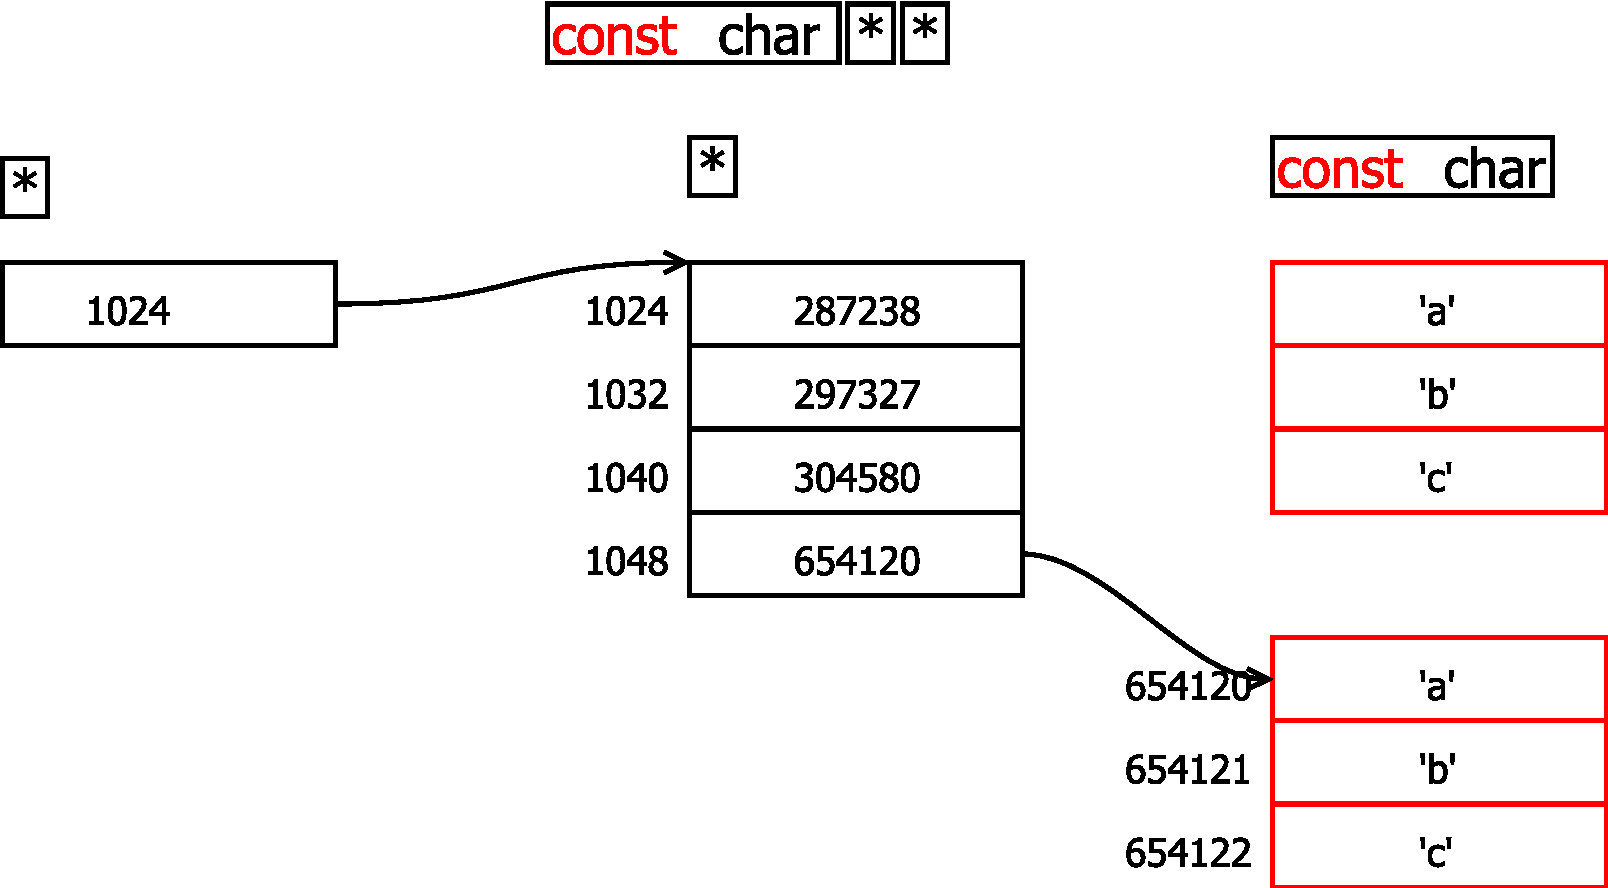
\includegraphics[width=\linewidth]{const_char_pointer_pointer}
    \caption{Puntero a carácter constante}
    \label{img:constcharpointerpointer}
\end{figure}

\begin{figure}[H]
    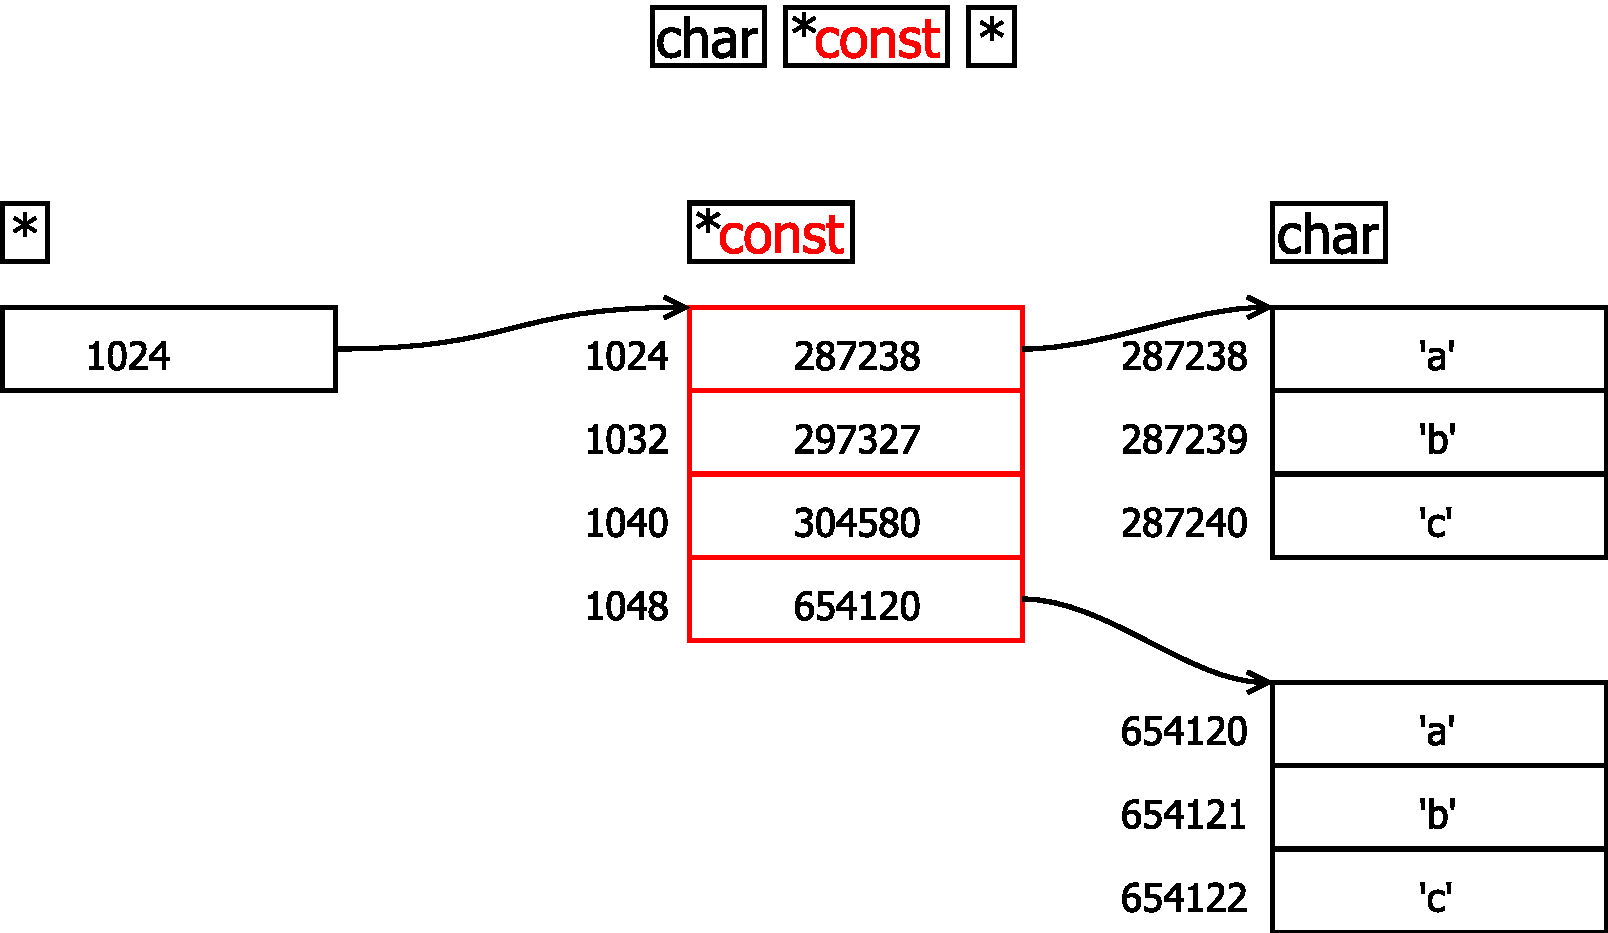
\includegraphics[width=\linewidth]{char_pointer_const_pointer}
    \caption{Puntero a puntero constante a \texttt{char}}
    \label{img:charconstpointerpointer}
\end{figure}

Vamos a explicarlo despacio, si miras el primer dibujo, es <<a lo que estamos
acostumbrados>>, cada asterisco es un nuevo nivel de puntero, así que puedes
leer la declaración desde la izquierda y construirá los tipos. Empecemos:
nos encontramos \verb!const!, lo que venga ahora es constante, después
\verb!char!, ahora llega un asterisco, el asterisco inicia un nuevo nivel, así
que este puntero \textbf{no} será constante, porque no tiene un \verb!const!
a la derecha y, finalmente, otro nivel de puntero, que tampoco será constante.
Ahora que ya tienes los tres grupos, los inviertes, es decir: puntero no
constante, a puntero no contante, a \verb!char! constante.

En el caso siguiente tenemos un \verb!char!, después un asterisco, es decir,
un nivel de puntero, lleva const a la derecha, así que es constante, y después
otro puntero, sin constancia. Es decir, invirtiéndolo: puntero no constante a
puntero constante a char no constante. En ambos casos, en el diagrama, he
señalado en rojo los valores que no puedes cambiar, como puedes ver, en el
superior no podemos cambiar los \textit{strings}, pero sí los punteros
intermedios. En el caso de abajo, por el contrario, podemos modificar los
caracteres, pero no los punteros del array intermedio.

Una de las implicaciones de las funciones genéricas es la siguiente: se
introduce una sobrecarga inevitable, por dos motivos. El primero es que las
funciones que utilizan punteros a \verb!void! tienen que hacer cálculos
explícitos que se harían implícitamente. No voy a entrar en detalles de
arquitectura de computadores, pero los ordenadores tienen en sus procesadores
instrucciones que manejan datos como enteros de cuatro bytes y números decimales
(y algunos más). Al tener que copiar byte a byte, impedimos que se utilicen y,
además, tenemos que darle más vueltas al bucle de copia, lo cual es más costoso.
El segundo es que cuando se llama a una función de manera normal el
compilador cuenta con ello para saber cómo generar el binario. Cuando ésta
es un argumento, esta tarea se le hace más complicada, porque no sabe qué
función es hasta el momento de la ejecución. Para hacer esto patente, vamos
a hacer una comparación con el tiempo que tarden ambas versiones en ordenar
65.536 y 131.072 elementos. Vamos a comparar ambas cargas de trabajo porque
quiero que veas una cosa.

\begin{table}[H]
\begin{tabularx}{\linewidth}{|c|R|R|}
\hline
\textbf{Función}&\textbf{N=35.536}&\textbf{N=131.072}\\\hline
Específica&16,21&64,61\\\hline
Genérica&41,20&164,44\\\hline
\textbf{Ratio}&0,39&0,39\\\hline
\end{tabularx}
\caption{Tiempos de ejecución de los distintos algoritmos}
\label{tab:sortingTimes}
\end{table}

Como puedes ver, la versión genérica tarda más, pero he calculado un dato
importante a ese respecto: el ratio entre el tiempo del algoritmo específico y
el algoritmo genérico. Como puedes ver, aunque el algoritmo genérico es peor
que el específico, la buena noticia es que esa diferencia es constante, es
decir: no empeora con el tamaño del vector. Esto hace que, si podemos asumir
el aumento de tiempo, la solución sea escalable, que es una manera que se tiene
en informática de decir que puedes hacer crecer algo sin quedarte sin recursos
rápidamente.

Un ejercicio muy interesante sería que programaras la versión genérica de
\textit{Quick Sort} y que, además, hicieras estas mismas mediciones. Para
medir el tiempo puedes utilizar este código:

\noindent
\begin{minipage}[H]{\linewidth}
\mbox{}
\begin{lstlisting}[style=C,
caption={Cómo medir el tiempo},
label={lst:measure_times}]
#include <stdio.h>
#include <time.h>

double timespec_to_double(const struct timespec* tm)
{
    return tm->tv_sec + tm->tv_nsec / 1000000000.0;
}

int main(int argc, char** argv)
{
    double start, stop;
    struct timespec start_ts, stop_ts;

    clock_gettime(CLOCK_REALTIME, &start_ts);
    start = timespec_to_double(&start_ts);
    // Aquí el código que quieres medir.
    clock_gettime(CLOCK_REALTIME, &stop_ts);
    stop = timespec_to_double(&stop_ts);
    printf("Hemos tardado: %lf\n", stop - start);
}
\end{lstlisting}
\end{minipage}

La función \verb!clock_gettime! es una función para medir el tiempo de un modo
peculiar, en sistemas Linux se mide el tiempo desde el primero de enero de
1970. Así, la estructura \verb!timespec! indica el tiempo pasado desde entonces
como un conjunto de segundos más los correspondientes nanosegundos en sus dos
miembros. Como eso es poco práctico he creado una pequeña función para
convertirlo a número decimal y así poder restarlo cómodamente. Después,
simplemente mido el tiempo antes y después del código que quiero saber cuánto
tarda y los resto, como puedes ver.

\section{Ejemplo completo de programa}
Esta sección está al final porque, si hasta ahora hemos visto cada parte del
lenguaje en detalle y por sí misma, en esta vamos a intentar montar todas las
piezas en una gran fotografía. Para esto vamos a utilizar y refinar un ejemplo
que ha sido recurrente en el manual: la gestión de una estructura que almacena
los datos de una persona, pero vamos a conseguir separar bien al usuario de la
funcionalidad interna del código que se encague de eso.

Lo que haremos es crear un archivo de código fuente llamado \verb!person.c! y
su correspondiente archivo de cabeceras, \verb!person.h!, en este archivo
incluiremos funcionalidad para crear una estructura persona, cambiar
sus atributos, leerlos y serializarla. Además, vamos a ver un interesante
artefacto del lenguaje para poder impedir que el usuario se entrometa en
nuestra estructura y pueda alterar los datos de manera incorrecta. Por ejemplo:
asignando los punteros a una zona de memoria que no controlemos desde estas
funciones proporcionadas para manipular la estructura de datos.

Lo primero que voy a hacer es crear el archivo de cabeceras porque ya hemos
definido de una manera muy concreta la funcionalidad de este código fuente.
Aquí hay una cosa interesante que podremos comentar, veamos el archivo:

\noindent
\begin{minipage}[H]{\linewidth}
\mbox{}
\begin{lstlisting}[style=C,
caption={Ejemplo final de programa -- \texttt{person.h}},
label={lst:finalExPerson_h}]
#ifndef PERSON_H
#define PERSON_H

typedef struct person_s person_t;

person_t *create_person(const char *name, const char *last_name,
                        unsigned int age);

void destroy_person(person_t *p);

void person_set_name(person_t *p, const char *name);

void person_set_last_name(person_t *p, const char *last_name);

void person_set_age(person_t *p, unsigned int age);

const char *person_get_name(const person_t *person);

const char *person_get_last_name(const person_t *person);

unsigned int person_get_age(const person_t *person);

char *person_to_string(const person_t *p);

#endif
\end{lstlisting}
\end{minipage}

Y aquí puedes ver una de las cosas interesantes de este ejemplo final: estamos
declarando el tipo \verb!person_t!, pero no el \textit{struct} al que da nombre,
esto quiere decir que cualquier archivo de código fuente que incluya este
\textbf{no} podrá saber la definición de tal \textit{struct}. La implicación de
esto es que no podrá declarar variables de este tipo, tan solo punteros, puede
declarar un puntero, porque todos los punteros tienen el mismo tamaño. Si
intentáramos declarar una variable de este tipo, el compilador lanzaría un error
como el siguiente:

\noindent
\begin{minipage}[H]{\linewidth}
\mbox{}
\begin{lstlisting}[style=terminalStyle]
main.c: In function 'main':
main.c:5:14: error: storage size of 'francis' isn't known
    5 |     person_t francis;
      |              ^~~~~~~
\end{lstlisting}
\end{minipage}

Este es el mecanismo que nos permite impedir que el usuario altere el contenido
de la estructura fuera de nuestro control (como comentamos en el programa
\ref{lst:structConstMain}) porque, del mismo modo que no conoce el tamaño del tipo,
tampoco conoce los miembros de esta estructura, así que no puede accederse a
ellos. Nota, además, como no hemos incluido ninguna cabecera en \verb!person.h!.
Si necesitáramos cabeceras, por ejemplo, la cabecera \verb!stdint.h! contiene
definiciones de tipo útiles como aquéllos de tamaño fijo: \verb!int8_t!,
\verb!int16_t!, etc.; si quisiéramos definir alguna función con un argumento
de este tipo o de tipo de retorno, sí sería necesario que incluyéramos esta
cabecera. Si las necesitamos en las implementaciones (en las declaraciones de
esctructuras, en las definiciones de funciones...), será en el archivo de
código fuente (en el \verb!.c!) donde las incluiremos.

El siguiente archivo es, precisamente, este archivo de código fuente:
\verb|person.c|. Es bastante largo, así que vamos a incluirlo en tres secciones:
la sección de declaración de tipos (que sólo contendrá uno), las funciones de
manipulación del contenido de la estructura y, finalmente, la de recuperación
de la información.

\noindent
\begin{minipage}[H]{\linewidth}
\mbox{}
\begin{lstlisting}[style=C, label={lst:finalExDefinition},
caption={Ejemplo final de programa -- \texttt{person.c} definiciones}]
#include <string.h> //strdup, memset
#include <stdlib.h> //malloc
#include <stdio.h>  //snprintf
#include "person.h"

struct person_s
{
    char *name;
    char *last_name;
    unsigned int age;
};

person_t *create_person(const char *name,
                        const char *last_name,
                        unsigned int age)
{
    person_t *res = malloc(sizeof(*res));
    memset(res, 0, sizeof(*res));

    res->age = age;
    res->name = strdup(name);
    res->last_name = strdup(last_name);

    return res;
}

void destroy_person(person_t *p)
{
    free(p->name);
    free(p->last_name);
    free(p);
}
\end{lstlisting}
\end{minipage}

Aquí podemos ver la defininión del tipo del que en la cabecera hicimos un
\verb!typedef!, este estilo de declaración de un tipo se llama declaración
anticipada o, en inglés, \textit{forwarding declaration}. Aquí, aparte de la
definición del tipo propiamente dicho, tenemos las funciones que lo crean
y que lo destruyen. Como esta estructura contiene elementos reservados con
memoria dinámica, debemos proveer al usuario una manera de liberar los recursos
de la estructura. Como puedes ver, en las funciones de creación reservamos
espacio \textbf{para la propia estructura} y para sus campos.

Debemos reservar
nosotros dinámicamente la estructura aparte de sus campos porque, recordemos,
fuera de este archivo de código fuente no podremos declarar más que punteros,
y ese puntero no tendrá espacio para nada si no lo declaramos. Después,
reservamos memoria para el contenido al que apuntarán los \textbf{miembros}
de la estructura.
En la función de destrucción, simétricamente, liberamos primero los contenidos
y después la propia estructura. Nota, además, cómo hemos declarado todos los
argumentos que hemos podido como constantes, para que el usuario no tenga dudas
de si vamos a modificar datos que nos proporcione.

Las siguientes funciones son las que nos permiten sobreescribir los datos:

\noindent
\begin{minipage}[H]{\linewidth}
\mbox{}
\begin{lstlisting}[style=C, label={lst:finalExSetter},
caption={Ejemplo final de programa -- \texttt{person.c} manipulación}]
void person_set_name(person_t *p, const char *name)
{
    free(p->name);
    p->name = strdup(name);
}

void person_set_last_name(person_t *p, const char *last_name)
{
    free(p->last_name);
    p->last_name = strdup(last_name);
}

void person_set_age(person_t *p, unsigned int age)
{
    p->age = age;
}
\end{lstlisting}
\end{minipage}

Como puedes ver, las funciones son simples, liberamos la memoria de los campos
y después le asignamos la duplicación del argumento que se nos pasa. De nuevo,
observa cómo hemos definido como constantes los argumentos del mismo modo que
hicimos en la función de creación. Las funciones no devuelven nada (\verb!void!)
porque no tendríai sentido. Aunque siempre podrían devolver un entero que
actuara como código de error, por ejemplo si la reserva de memoria fallara,
se podría indicar devolviendo un número menor que cero.

\noindent
\begin{minipage}[H]{\linewidth}
\mbox{}
\begin{lstlisting}[style=C, label={lst:finalExGetter},
caption={Ejemplo final de programa -- \texttt{person.c} recuperación}]
const char *person_get_name(const person_t *p)
{
    return p->name;
}

const char *person_get_last_name(const person_t *person)
{
    return person->last_name;
}

unsigned int person_get_age(const person_t *person)
{
    return person->age;
}

char *person_to_string(const person_t *p)
{
#define MAX_STRING_SIZE ((unsigned int)1024)

    char res[MAX_STRING_SIZE + 1];
    snprintf(res, MAX_STRING_SIZE, "{\"name\":\"%s\","
                                   "\"last_name\":\"%s\","
                                   "\"age\":%u}",
             p->name, p->last_name, p->age);
    return strdup(res);
#undef MAX_STRING_SIZE
}
\end{lstlisting}
\end{minipage}

Aquí debes notar que devolvemos punteros contantes a \verb!char!, precisamente
para impedir que el usuario libere, manipule o cambie el contenido de los campos
del \textit{struct}. Sin embargo; en la función de serialización (que he
reducido a su versión más simple) devuelvo un puntero no constante porque la
responsabilidad de liberar es del usuario de la funcionalidad, no de esta
biblioteca. Además, en esta última función puedes ver que podemos
\textbf{eliminar} una macro con la directiva \verb!#undef!. Esto es útil cuando
necesitas inicializar un array, como aquí, pero no quieres contaminar de
símbolos el código fuente. Así, si otra función usara strings de otro tamaño,
podríamos usar el mismo nombre, como si la macro fuera una variable distinta.
De nuevo: ten cuidado, las macros trabajan a nivel de preprocesado, por lo que
no estás definiendo ninguna variable en la función, sólo una región de código
donde un símbolo se sustituirá por otro.

Finalmente, en el archivo principal podemos utilizar la funcionalidad:

\noindent
\begin{minipage}[H]{\linewidth}
\mbox{}
\begin{lstlisting}[style=C, label={lst:finalExMain},
caption={Ejemplo final de programa -- \texttt{main.c}}]
#include "person.h"
#include <stdlib.h>
#include <stdio.h>

int main(void)
{
    person_t* person = create_person("John", "Smith", 18);

    char* serialization = person_to_string(person);

    printf("%s\n", serialization);
    free(serialization);

    person_set_name(person, "Michael");
    person_set_last_name(person, "Johnson");
    person_set_age(person, 33);

    serialization = person_to_string(person);
    printf("%s\n", serialization);
    free(serialization);
}
\end{lstlisting}
\end{minipage}

Aquí se puede ver cómo se utilizan estructuras con este patrón de diseño.
Primero la reservas, después la usas, la puedes manipular y, finalmente, la
liberas, todo ello con las funciones proporcionadas junto con el tipo de dato.
Con este patrón, el usuario de la funcionalidad que hemos programado tiene
menos capacidad para <<hacer algo mal>>.

Ahora, vamos a ver rápidamente cómo se podría compilar, para recordarlo. Primero
lo haremos utilizando el código objeto y, después, crearemos una biblioteca
dinámica y la enlazaremos. Para compilar utilizando el código
objeto seguiremos estos pasos:

\noindent
\begin{minipage}[H]{\linewidth}
\begin{enumerate}
\item Crear el código objeto de \verb!person.c!

\noindent
\begin{minipage}[H]{\linewidth}
\mbox{}
\begin{lstlisting}[style=terminalStyle]
\$ gcc -c person.c
\end{lstlisting}
\end{minipage}
\item Crear el código objeto de \verb!main.c!

\noindent
\begin{minipage}[H]{\linewidth}
\mbox{}
\begin{lstlisting}[style=terminalStyle]
\$ gcc -c main.c
\end{lstlisting}
\end{minipage}
\item Crear el ejecutable con ambos códigos objeto

\noindent
\begin{minipage}[H]{\linewidth}
\mbox{}
\begin{lstlisting}[style=terminalStyle]
\$ gcc -o main.exe main.o person.o -g -Wall -Wextra
\end{lstlisting}
\end{minipage}
\end{enumerate}
\end{minipage}

Para la biblioteca, seguiremos estos pasos:

\noindent
\begin{minipage}[H]{\linewidth}
\begin{enumerate}
\item Crear el código objeto de \verb!person.c!

\noindent
\begin{minipage}[H]{\linewidth}
\mbox{}
\begin{lstlisting}[style=terminalStyle]
\$ gcc -c person.c
\end{lstlisting}
\end{minipage}
\item Crear una biblioteca con este código objeto:

\noindent
\begin{minipage}[H]{\linewidth}
\mbox{}
\begin{lstlisting}[style=terminalStyle]
\$ gcc -shared -o libperson.so person.o
\end{lstlisting}
\end{minipage}
\item Crear el código objeto de \verb!main.c!

\noindent
\begin{minipage}[H]{\linewidth}
\mbox{}
\begin{lstlisting}[style=terminalStyle]
\$ gcc -c main.c
\end{lstlisting}
\end{minipage}
\item Crear el ejecutable usando la biblioteca:

\noindent
\begin{minipage}[H]{\linewidth}
\mbox{}
\begin{lstlisting}[style=terminalStyle]
\$ gcc -L. -Wl,-rpath=. -o main.exe main.o -lperson
\end{lstlisting}
\end{minipage}
\end{enumerate}
\end{minipage}

En este ejemplo final se han visto ejemplos de la mayoría de conceptos que
se han explicado en el manual: variables, punteros, memoria, reserva dinámica,
estructuras, macros, enlazado, compilación y constancia y signo. Es mucha
información en pocas páginas, pero permite tener una foto global de todo
si ya se ha leído antes con detenimiento.

%\subsection{Ejercicio de la sección}
%En esta sección voy a proponer un último ejercicio, pero detallado, que permita
%practicar todos o casi todos los conceptos vistos en el manual. El ejercicio es
%crear un proyecto que incluye las siguientes funcionalidades:
%\begin{itemize}
%\item Manejo de una estructura <<coordenada>> que permita almacenar
%una coordenada bidimensional (un punto) con un \textbf{nombre} que sea una
%cadena de texto. Esta cadena de texto debe manejarse con funciones que impidan
%que el usuario deje la estructura en un estado inconsistente.
%    \begin{itemize}
%    \item Debe poderse calcular la distancia entre dos puntos. Se recibirán
%    punteros y si uno de ellos o los dos es \verb!NULL! se tomará por el punto
%    de origen.
%    \item Debe poderse ordenar un vector de puntos por su distancia al origen.
%    Idealmente, debería usarse el algoritmo \textit{Quick Sort}.
%    \item Debe poderse cambiar el nombre de un punto si destruirlo y crearlo
%    de nuevo con una función para tal fin.
%    \end{itemize}
%\item Manejo de una estructura <<polígono>> que tenga un conjunto de puntos
%de los descritos anteriormente. Hay que tener en cuenta que cada punto estará
%conectado con el siguiente y el anterior; menos el último, que estará conectado
%al penúltimo y al primero, y el primero, que estará conectado al segundo y
%al último.
%    \begin{itemize}
%    \item Deberá poderse modificar un polígono añadiendo o eliminando puntos
%    al final.
%    \item Deberá poderse insertar un punto en una posición dada de un polígono.
%    \item Deberá poderse calcular el centro del polígono como la media de las
%    coordenadas de un punto.
%    \end{itemize}
%\item Se deben crear funciones que permitan hacer estas tareas con estructuras
%que simbolicen y aumenten las funcionalidades de los vectores,
%idealmente, de cualquier tipo:
%    \begin{itemize}
%    \item Insertar en cualquier posición
%    \item Insertar al final
%    \item Conocer la longitud del vector
%    \item Vaciar el vector
%    \item Eliminar un elemento de la posición del vector
%    \item Ordenar el vector
%    \item Crear un vector con una longitud dada, relleno de un valor concreto
%    \end{itemize}
%Las dos primeras funcionalidades deben estar en una biblioteca llamada
%\verb!libGeo.so! y la siguiente en \verb!libVector.so!. Se debe crear un
%programa que utilice todas las funcionalidades y las pruebe.
%\end{itemize}

\section{Anexo A: soluciones a ejercicios}
\begin{exercises}
\item Escribe un programa y declara en él una estructura que defina un círculo
en dos dimensiones (su centro y su radio). Y haz que el programa declare una
variable de ese tipo y calcule su área.


\noindent
\begin{minipage}[H]{\linewidth}
\mbox{}
\begin{lstlisting}[style=C,
caption={Solución al ejercicio 1},
label={lst:solution1}]
#include <stdio.h>

struct circle_s {
    double x;
    double y;
    double r;
};

int main(void)
{
    struct circle_s circle = { 1 , 1 , 3.4 };
    double area = 3.141592 * circle.r * circle.r;
    printf("El área del círculo en el punto [%f, %f] con un radio de % f es: %f\n", circle.x, circle.y, circle.r, area);
}
\end{lstlisting}
\end{minipage}

\item Haz un programa que, basándose en el struct punto presentado en el
ejemplo, declare e inicialice un array de ellos y vaya diciendo las direcciones
que hay que seguir para ir de uno a otro.


\noindent
\begin{minipage}[H]{\linewidth}
\mbox{}
\begin{lstlisting}[style=C,
caption={Solución al ejercicio 2},
label={lst:solution2}]
#include <stdio.h>
struct point_s {
    double x;
    double y;
};

int main(void)
{
    struct point_s points[10] = { {-1.056171, 3.401877},
                                  {2.984400, 2.830992},
                                  {-3.024486, 4.116474},
                                  {2.682296, -1.647772},
                                  {0.539700, -2.222253},
                                  {1.288709, -0.226029},
                                  {0.134009, -1.352155},
                                  {4.161951, 4.522297},
                                  {2.172969, 1.357117},
                                  {1.069689, -3.583974} };

    for(int ii = 1; ii < 10; ++ii){
        if (points[ii - 1].x < points[ii].x) {
            printf("Derecha");
        }else if(points[ii - 1].x == points[ii].x){
            printf("Quieto");
        }else if(points[ii - 1].x > points[ii].x){
            printf("Izquierda");
        }
        printf(", ");
        if (points[ii - 1].y < points[ii].y) {
            printf("Arriba");
        }else if(points[ii - 1].y == points[ii].y){
            printf("Quieto");
        }else if(points[ii - 1].y > points[ii].y){
            printf("Abajo");
        }
        printf("\n");
    }
}
\end{lstlisting}
\end{minipage}

\item Haz un programa que declare un array bidimensional y calcule la suma de
sus filas y sus columnas.


\noindent
\begin{minipage}[H]{\linewidth}
\mbox{}
\begin{lstlisting}[style=C,
caption={Solución al ejercicio 3},
label={lst:solution3}]
#include <stdio.h>

int main(void)
{
    int array[3][3] = { {1,3,6},{7,3,6},{1,2,4} };

    for (int ii = 0; ii < 3; ++ii) {
        for (int jj = 0; jj < 3; ++jj) {
            printf("%d ", array[ii][jj]);
        }
        int suma = 0;
        for(int jj = 0; jj < 3; ++jj){
            suma += array[ii][jj];
        }
        printf("= %d\n", suma);
    }
    for(int ii = 0; ii < 3*2; ++ii){
        printf("-");
    }
    printf("\n");
    for(int ii = 0; ii < 3; ++ii){
        int suma = 0;
        for(int jj = 0; jj < 3; ++jj){
            suma+=array[jj][ii];
        }
        printf("%d ", suma);
    }
    printf("\n");
}

\end{lstlisting}
\end{minipage}


\item Haz un programa que haga lo siguiente para los números del 1 al 100 ambos
incluidos: si el número es divisible entre 2, debe imprimirse por pantalla
<<fizz>>, si es divisible entre 5, <<buzz>>, y si es divisible entre los dos,
<<fizzbuzz>>, no imprimir nada en otro caso.


\noindent
\begin{minipage}[H]{\linewidth}
\mbox{}
\begin{lstlisting}[style=C,
caption={Solución al ejercicio 4},
label={lst:solution4}]
#include <stdio.h>

int main(void)
{
    for (int ii = 1; ii <= 100; ++ii){
        int end_of_line = 0;
        if (ii % 2 == 0){
            printf("fizz");
            end_of_line = 1;
        }

        if(ii % 5 == 0){
            printf("buzz");
            end_of_line = 1;
        }
        if(end_of_line){
            printf("\n");
        }
    }
}
\end{lstlisting}
\end{minipage}

\item Escribe una función que calcule si un número es primo o no.


\noindent
\begin{minipage}[H]{\linewidth}
\mbox{}
\begin{lstlisting}[style=C,
caption={Solución al ejercicio 5},
label={lst:solution5}]
#include <stdio.h>

int is_prime(int number) {
    int prime = 1;
    for (int ii = 2; ii < number / 2 && prime; ++ii) {
        if (0 == number % ii) {
            prime = 0;
        }
    }
    return prime;
}

int main(void)
{
    for(int ii = 2; ii < 100; ii++){
        printf("El número %d ", ii);
        if(is_prime(ii)){
            printf("es primo.");
        }else{
            printf("no es primo");
        }
        printf("\n");
    }
}
\end{lstlisting}
\end{minipage}

\item Escribe una función que calcule la distancia entre dos estructuras punto
de las usadas en la sección anterior.


\noindent
\begin{minipage}[H]{\linewidth}
\mbox{}
\begin{lstlisting}[style=C,
caption={Solución al ejercicio 6},
label={lst:solution6}]
#include <stdio.h>
#include <math.h>
struct point_s {
    double x;
    double y;
};

double distance(struct point_s a, struct point_s b) {
    double res = 0.0;
    double diff_x = a.x - b.x;
    double diff_y = a.y - b.y;
    res = sqrt(diff_x * diff_x + diff_y * diff_y);
    return res;
}

int main(void)
{
    struct point_s a = {1.2, 4.3};
    struct point_s b = {3.4, 5.5};
    printf("La distancia entre [%f, %f] y [%f, %f] es: %f\n", a.x, a.y, b.x, b.y, distance(a,b));
}
\end{lstlisting}
\end{minipage}

\item Escribe una función que reciba un array de enteros y un caracter separador
que imprima los elementos del array separados por ese caracter.


\noindent
\begin{minipage}[H]{\linewidth}
\mbox{}
\begin{lstlisting}[style=C,
caption={Solución al ejercicio 7},
label={lst:solution7}]
#include <stdio.h>
void print_separated(int array[], int array_size, char separator){
    for(int ii = 0; ii < array_size; ++ii){
        printf("%d%c", array[ii], separator);
    }
}

int main(void)
{
    int my_array[] = {1,2,3,4,5,6,7,8,9,0};
    print_separated(my_array, 10, '|');
    printf("\n");
}
\end{lstlisting}
\end{minipage}

\item Escribe una función que encapsule el programa
\ref{lst:linealSystemFinal}: \nameref{lst:linealSystemFinal}.
La función debe recibir los coeficientes de las ecuaciones
($a$, $b$, $c$, $d$, $e$ y $f$). Puede recibirlos por separado o en un array.
Para devolver el resultado puedes crear una estructura que simplemente tenga
dos \verb!double!.



\begin{lstlisting}[style=C,
caption={Solución al ejercicio 8},
label={lst:solution8}]
#include <stdio.h>

struct solution_s {
    double x;
    double y;
    int solved;
};

struct solution_s linear_system(int a, int b, int c, int d, int e, int f) {

    double divisor;
    struct solution_s res;
    res.solved = 1;
    if (a != 0 && d != 0) {
        divisor = (a * e - d * b);
        if (divisor == 0)
        {
            printf("El sistema es irresoluble .\n");
            res.solved = 0;
        }
        else
        {
            res.y = (a * f - d * c) / divisor;
            res.x = (f - e * res.y) / (d);
        }
    }
    else if (b != 0 && e != 0) {
        divisor = (b * d - e * a);
        if (divisor == 0) {
            printf("El sistema es irresoluble .\n");
            res.solved = 0;
        }
        else {
            res.x = (b * f - e * c) / divisor;
            res.y = (c - a * res.x) / b;
        }
    }
    else if ((a == 0 && b == 0) || (d == 0 && e == 0)) {
        printf(" Esto no es un sistema \n");
        res.solved = 0;
    }
    else {
        if (a != 0) {
            res.x = (double)c / a;
            res.y = (double)f / e;
        }
        else {
            res.x = (double)f / d;
            res.y = (double)c / b;
        }
    }
    return res;
}


int main(void)
{
    struct solution_s sol = linear_system(1, 1, 1, 2, 2, 2);
    printf(" %dx+ %dy= %d\n", 1, 2, 3);
    printf(" %dx+ %dy= %d\n", 4, 5, 6);
    if (sol.solved) {
        printf("x = %f; y = %f\n", sol.x, sol.y);
    }
    else {
        printf("El sistema no tiene solucion.\n");
    }
}
\end{lstlisting}


\item Escribe una función que normalice los elementos de un array de
\verb!double!.

\noindent
\begin{minipage}[H]{\linewidth}
\mbox{}
\begin{lstlisting}[style=C,
caption={Solución al ejercicio 9},
label={lst:solution9}]
#include <stdio.h>

void normalize(double array[], int array_size) {
    double biggest = array[0];
    for (int ii = 1; ii < array_size; ++ii) {
        if (array[ii] > biggest) {
            biggest = array[ii];
        }
    }
    for (int ii = 0; ii < array_size; ++ii) {
        array[ii] /= biggest;
    }
}

int main(void)
{
    double array[] = { 1,2,3,4,5,6,7,8,9,10 };
    normalize(array, 10);
    for(int ii = 0; ii < 10; ++ii){
        printf("%f\n", array[ii]);
    }
    printf("\n");
}
\end{lstlisting}
\end{minipage}

\item Completa esta tabla de números en diferentes bases numéricas:
\begin{table}[H]
\begin{tabularx}{\linewidth}{|R|R|R|}
\hline
\multicolumn{1}{|Y|}{\textbf{Decimal}}& \multicolumn{1}{Y|}{\textbf{Binario}} & \multicolumn{1}{Y|}{\textbf{Hexadecimal}} \\\hline
73& 0100~1001 & 0x049 \\\hline
 38&0010~0110&0x026 \\\hline
303&0001~0010~1111&0x12F       \\\hline
128&1000~0000&0x080 \\\hline
\end{tabularx}
\end{table}
\item Vuelve al ejercicio noveno y reproduce los contenidos de la pila en cada
bloque de código del programa. Utiliza de referencia la solución que propongo
yo.

\begin{stack}
    \item Función main
    \begin{stack}
        \item Array (10 elementos)
        \item Entramos en la función normalize
        \begin{stack}
            \item Array (puntero a)
            \item \verb!array_size!
            \item \verb!biggest!
            \item Primer bucle for
            \begin{stack}
                \item \verb!ii!
            \end{stack}
            \item Segundo bucle for
            \begin{stack}
                \item \verb!ii!
            \end{stack}
        \end{stack}
        \item Bucle for
        \begin{stack}
            \item \verb!ii!
        \end{stack}
    \end{stack}
\end{stack}

\item Haz un programa que cree un puntero de tres niveles de tipo \verb!int!,
lo reserve correctamente, lo rellene con el valores correlativos
\textbf{empezando en uno} y después lo imprima de una manera comprensible.
Finalmente, libéralo también de tal modo que no quede memoria sin liberar al
final del programa.

\noindent
\begin{minipage}[H]{\linewidth}
\mbox{}
\begin{lstlisting}[style=C,label=lst:solution12, caption={Solución al ejercicio 12}]
#include <stdio.h>
#include <stdlib.h>

#define DEPTH (10)
#define WIDTH (5)
#define HEIGHT (12)

int main(int argc, char const *argv[]) {
    int ***cube = malloc(sizeof(*cube) * DEPTH);

    for (int ii = 0; ii < DEPTH; ++ii) {
        cube[ii] = malloc(sizeof(**cube) * HEIGHT);
        for (int jj = 0; jj < HEIGHT; ++jj) {
            cube[ii][jj] = malloc(sizeof(***cube) * WIDTH);
            for (int kk = 0; kk < WIDTH; ++kk) {
                cube[ii][jj][kk] =
                    kk + jj * WIDTH + ii * HEIGHT * WIDTH + 1;
            }
        }
    }

    for (int ii = 0; ii < DEPTH; ++ii) {
        for (int jj = 0; jj < HEIGHT; ++jj) {
            for (int kk = 0; kk < WIDTH; ++kk) {
                printf("%3d ", cube[ii][jj][kk]);
            }
            printf("\n");
        }
        printf("\n");
    }

    for (int ii = 0; ii < DEPTH; ++ii) {
        for (int jj = 0; jj < HEIGHT; ++jj) {
            free(cube[ii][jj]);
        }
        free(cube[ii]);
    }
    free(cube);

    return 0;
}
\end{lstlisting}
\end{minipage}


\item Basándote en el programa anterior, crea dos funciones, una para crear
una matriz tridimensional con memoria dinámica dadas sus tres dimensiones y
otra para liberarla.

\noindent
\begin{minipage}[H]{\linewidth}
\mbox{}
\begin{lstlisting}[ style=C,
                    label=lst:solution12,
                    caption={Solución al ejercicio 13 -- reserva}]
int ***malloc_cube(size_t depth, size_t height, size_t width) {
    int ***cube = malloc(sizeof(*cube) * depth);

    for (int ii = 0; ii < depth; ++ii) {
        cube[ii] = malloc(sizeof(**cube) * height);
        for (int jj = 0; jj < height; ++jj) {
            cube[ii][jj] = malloc(sizeof(***cube) * width);
            for (int kk = 0; kk < width; ++kk) {
                cube[ii][jj][kk] =
                    kk + jj * width + ii * height * width + 1;
            }
        }
    }
    return cube;
}
\end{lstlisting}
\end{minipage}

\noindent
\begin{minipage}[H]{\linewidth}
\mbox{}
\begin{lstlisting}[ style=C,
                    label=lst:solution12,
                    caption={Solución al ejercicio 13 -- impresión}]
void print_cube(int ***cube, size_t depth, size_t height,
                size_t width) {
    for (int ii = 0; ii < depth; ++ii) {
        for (int jj = 0; jj < height; ++jj) {
            for (int kk = 0; kk < width; ++kk) {
                printf("%3d ", cube[ii][jj][kk]);
            }
            printf("\n");
        }
        printf("\n");
    }
}
\end{lstlisting}
\end{minipage}

\noindent
\begin{minipage}[H]{\linewidth}
\mbox{}
\begin{lstlisting}[ style=C,
                    label=lst:solution12,
                    caption={Solución al ejercicio 13 -- liberación}]
void free_cube(int ***cube, size_t depth, size_t height,
               size_t width) {
    for (int ii = 0; ii < depth; ++ii) {
        for (int jj = 0; jj < height; ++jj) {
            free(cube[ii][jj]);
        }
        free(cube[ii]);
    }
    free(cube);
}
\end{lstlisting}
\end{minipage}

\noindent
\begin{minipage}[H]{\linewidth}
\mbox{}
\begin{lstlisting}[ style=C,
                    label=lst:solution12,
                    caption={Solución al ejercicio 13 -- función \texttt{main}}]
int main(int argc, char const *argv[]) {
    int ***cube = malloc_cube(DEPTH, HEIGHT, WIDTH);
    print_cube(cube, DEPTH, HEIGHT, WIDTH);
    free_cube(cube, DEPTH, HEIGHT, WIDTH);
}
\end{lstlisting}
\end{minipage}

\item Escribe un programa que reciba un número variable de números como
argumentos e imprima la descomposición en factores primos de todo ellos.
Se recomienda hacer control de errores comprobando que los argumentos son
números antes de utilizarlos, etc.

\noindent
\begin{minipage}[H]{\linewidth}
\mbox{}
\begin{lstlisting}[ style=C,
                    label=lst:solution12,
                    caption={Solución al ejercicio 13 -- función \texttt{main}}]
int main(int argc, char const *argv[]) {
    int ***cube = malloc_cube(DEPTH, HEIGHT, WIDTH);
    print_cube(cube, DEPTH, HEIGHT, WIDTH);
    free_cube(cube, DEPTH, HEIGHT, WIDTH);
}
\end{lstlisting}
\end{minipage}

\item Escribe un programa que lea \textbf{por consola} una serie de palabras
y que sólo deje de leer cuando se introduzca <<!!>> como palabra. Después, debe
imprimir dichas palabras en orden aleatorio. La función \verb!rand! devuelve
un número aleatorio entre cero y el máximo entero positivo. Si quieres que
devuelva números aleatorios \textbf{distintos} cada vez debes ejecutar
\verb!srand(time(NULL));! al inicio de la función \verb!main!. Debes incluir la
cabecera \verb!time.h!.

\noindent
\begin{minipage}[H]{\linewidth}
\mbox{}
\begin{lstlisting}[ style=C,
                    label=lst:solution12,
                    caption={Solución al ejercicio 15}]
#include <stdio.h>
#include <stdlib.h>
#include <string.h>
#include <time.h>

#define STRING_SIZE (1024)
#define MAX_WORDS (1024)

int main(int argc, char const *argv[]) {
    char *word_set[1024];
    int word_length = 0;
    do {
        word_set[word_length] = malloc(STRING_SIZE);
        scanf("%s", word_set[word_length]);
        word_length++;
    } while (strcmp(word_set[word_length - 1], "!!"));

    srand(time(NULL));
    for (int ii = 0; ii < word_length - 1; ++ii) {
        char *aux            = word_set[ii];
        int rand_index       = rand() % (word_length - 1);
        word_set[ii]         = word_set[rand_index];
        word_set[rand_index] = aux;
    }
    for (int ii = 0; ii < word_length - 1; ++ii) {
        printf("%s\n", word_set[ii]);
        free(word_set[ii]);
    }
    free(word_set[word_length-1]);
}
\end{lstlisting}
\end{minipage}

Como nota, para <<barajar>> el vector de palabras lo que hago el recorrerlo
intercambiando cada palabra con una posición aleatoria. Hay otros métodos
que quizás hayas usado como generar una posición aleatoria del vector y copiarlo
a otro, el problema de esto es que si lo que haces es generar un índice nuevo
cuando encuentras que ya has copiado ese, el número de veces que ejecutas
el aleatorio es, lógicamente, impredecible. Tal y como lo he escrito yo el
algoritmo siempre tardará lo mismo generando resultados moderadamente
aleatorios.

\item Haz una función que lea dos archivos e \textbf{intercambie} su contenido,
escribe dicho programa de tal modo que no sea necesario alojar ninguno de los
dos archivos en memoria completamente.

\newpage
\begin{lstlisting}[ style=C,
                    label=lst:solution16,
                    caption={Solución al ejercicio 16}]
#include <stdio.h>
#include <stdlib.h>

int main(int argc, char const *argv[]) {
    FILE *file_1 = NULL, *file_2 = NULL, *file_aux = NULL;
    const int BLOCK_SIZE = 1024;
    int read             = 0;
    char buffer[BLOCK_SIZE], aux_file_path[] = "/tmp/auxFile.txt";
    if (argc < 3) {
        printf("Uso: main.exe <archivo1> <archivo2>\n");
        return EXIT_FAILURE;
    }

    file_1 = fopen(argv[1], "r+");
    if (NULL == file_1) {
        printf("ERROR: El primer archivo no existe.\n");
        return EXIT_FAILURE;
    }

    file_2 = fopen(argv[2], "r+");
    if (NULL == file_2) {
        printf("ERROR: El segundo archivo no existe.\n");
        fclose(file_1);
        return EXIT_FAILURE;
    }

    file_aux = fopen(aux_file_path, "w+");
    if (NULL == file_aux) {
        fclose(file_1);
        fclose(file_2);
        return EXIT_FAILURE;
    }

    // copy file 1 to aux
    while (read = fread(buffer, sizeof(char), BLOCK_SIZE, file_1)) {
        fwrite(buffer, sizeof(char), read, file_aux);
    }
    fclose(file_1);
    file_1 = fopen(argv[1], "w+");
    if (NULL == file_1) {
        printf("Error, el primer archivo no se ha podido reabrir\n");
    }

    // copy file 2 to 1
    while (read = fread(buffer, sizeof(char), BLOCK_SIZE, file_2)) {
        fwrite(buffer, sizeof(char), read, file_1);
    }

    fclose(file_2);
    file_2 = fopen(argv[2], "w+");
    if (NULL == file_2) {
        printf("Error, el segundo archivo no se ha podido reabrir\n");
    }

    // copy aux file to file 2, we need to go back to begin of file aux
    fseek(file_aux, 0, SEEK_SET);
    while (read = fread(buffer, sizeof(char), BLOCK_SIZE, file_aux)) {
        fwrite(buffer, sizeof(char), read, file_2);
    }

    fclose(file_1);
    fclose(file_2);
    fclose(file_aux);
    remove(aux_file_path);
}
\end{lstlisting}

\item Escribe una función que reciba una palabra como argumento e indique
en qué posición (en bytes) dentro del archivo se encuentra la palabra. Sólo
tienes que dar la primera ocurrencia, si la palabra no se encuentra, devuelve
un número negativo. Haz un programa que, con esa función, reciba una ruta a un
archivo y una palabra e imprima el resultado de buscar la palabra en el archivo.

\noindent
\begin{minipage}[H]{\linewidth}
\mbox{}
\begin{lstlisting}[style=C,
caption={Solución al ejercicio 17},
label={lst:solution17}]
#include <stdio.h>
#include <stdlib.h>
#include <string.h>

int find_in_file(const char *path, const char *word) {
    FILE *file = NULL;
    char *buffer;
    int word_length = 0, read = 0, pos = -1;

    file = fopen(path, "r+");
    if (NULL == file) {
        printf("ERROR: El archivo no existe.\n");
        return -1;
    }
    word_length = strlen(word);
    buffer      = malloc(sizeof(char) * word_length * 2);

    while (read = fread(buffer, sizeof(char), word_length * 2, file)) {
        fseek(file, word_length - read, SEEK_CUR);
        for (int ii = 0; ii < word_length; ++ii) {
            char local_word[word_length + 1];
            memcpy(local_word, buffer + ii, word_length);
            local_word[word_length] = 0;
            if (!strcmp(local_word, word)) {
                pos = ftell(file) + ii - word_length;
                goto end;
            }
        }
    }
end:
    free(buffer);
    fclose(file);
    return pos;
}

int main(int argc, char const *argv[]) {

    int pos = find_in_file(argv[1], argv[2]);
    printf("La palabra %s está en la posición %d en el archivo %s\n",
           argv[2], pos, argv[1]);
}
\end{lstlisting}
\end{minipage}

Aquí puedes ver un uso típico de la instrucción \verb!goto!, como necesitamos
hacer lo mismo encontremos la palabra o no, lo que hacemos es establecer
una etiqueta y saltar allí para liberar recursos y devolver el resultado.

\item Reescribe el ejercicio 15 prescindiendo del array estático de punteros
a \verb!char!. (Usa \verb!realloc! y \verb!strdup!.

\noindent
\begin{minipage}[H]{\linewidth}
\mbox{}
\begin{lstlisting}[style=C,
caption={Solución al ejercicio 18},
label={lst:solution18}]
#include <stdio.h>
#include <stdlib.h>
#include <string.h>
#include <time.h>

int main(int argc, char const *argv[]) {
    char word[1024];
    char **word_set = NULL;
    int word_length = 0;
    do {
        word_set = realloc(word_set, ++word_length * sizeof(char *));
        scanf("%s", word);
        word_set[word_length - 1] = strdup(word);
    } while (strcmp(word, "!!"));

    srand(time(NULL));
    for (int ii = 0; ii < word_length - 1; ++ii) {
        char *aux            = word_set[ii];
        int rand_index       = rand() % (word_length - 1);
        word_set[ii]         = word_set[rand_index];
        word_set[rand_index] = aux;
    }
    for (int ii = 0; ii < word_length - 1; ++ii) {
        printf("%s\n", word_set[ii]);
    }
    for (int ii = 0; ii < word_length; ++ii) {
        free(word_set[ii]);
    }
    free(word_set);
}
\end{lstlisting}
\end{minipage}


\item Escribe un programa que reciba un número indeterminado de palabras como
argumentos y los ordene alfabéticamente y que, después, los imprima.


\noindent
\begin{minipage}[H]{\linewidth}
\mbox{}
\begin{lstlisting}[style=C,
caption={Solución al ejercicio 19},
label={lst:solution19}]
void generic_swap(void *one, void *other, size_t type_size) {
//...

void generic_bubble_sort(void *array, size_t array_size,
//...

int compare_strings(const void *one, const void *two) {
//...

int compare_strings(const void* one, const void* two) {
//...

int main(int argc, char const *argv[]) {

    generic_bubble_sort(argv + 1, argc - 1, sizeof(char *),
                        compare_strings);

    for (int ii = 1; ii < argc; ++ii) {
        printf("%s\n", argv[ii]);
    }
}
\end{lstlisting}
\end{minipage}

He usado las funciones de ejemplo para ordenar, así que omito su contenido,
simplemente tenemos que utilizar el comparador adecuado y tener en cuenta que
el primer argumento es el nombre de programa, que no queremos ordenar. Además,
puedes ver que podemos modificar el orden de los argumentos, pero no su
contenido, al haber declarado \texttt{argv} como \verb!char const*argv[]! que
quiere decir un array (puntero) no constante a \verb!char! constante. Es decir,
como ya vimos en la figura \ref{img:constcharpointerpointer}.


\item Haz un programa que reciba como argumento una palabra y un número. Si el
número es cero, debe convertir la palabra a minúscula, si el número es distinto
de cero, debe convertirla a mayúscula.

\noindent
\begin{minipage}[H]{\linewidth}
\mbox{}
\begin{lstlisting}[style=C,
caption={Solución al ejercicio 20},
label={lst:solution20}]
#include <stdio.h>
#include <stdlib.h>

char char_to_upper_case(char c) {
    if (c < 123 && c > 96) {
        return c - 32;
    }
    return c;
}

char char_to_lower_case(char c) {
    if (c < 91 && c > 64) {
        return c + 32;
    }
    return c;
}

char string_to_upper_case(char *message) {
    int length = strlen(message);
    for (int ii = 0; ii < length; ++ii) {
        message[ii] = char_to_upper_case(message[ii]);
    }
}

char string_to_lower_case(char *message) {
    int length = strlen(message);
    for (int ii = 0; ii < length; ++ii) {
        message[ii] = char_to_lower_case(message[ii]);
    }
}

int main(int argc, char const *argv[]) {

    char *message = strdup(argv[1]);
    int code = atoi(argv[2]);
    if(code){
        string_to_upper_case(message);
    }else{
        string_to_lower_case(message);
    }
    printf("%s\n", message);
    free(message);
}
\end{lstlisting}
\end{minipage}

Aquí hemos utilizado dos funciones diferentes para poner a mayúscula y
minúscula, otra opción sería utilizar un parámetro lógico (o incluso un
enumerado) para indicar qué tipo de letras se quiere y llamar a una función
que reciba ese parámetro y actúe en consecuencia. Puedes implementarlo así
como ejercicio extra.

\item Crea un programa que dado un número como argumento imprima una pirámide
como esta de tantos pisos como el número indicado.

\noindent
\begin{minipage}[H]{\linewidth}
\mbox{}
\begin{lstlisting}[style=C,
caption={Solución al ejercicio 21},
label={lst:solution21}]
#include <stdio.h>
#include <stdlib.h>
#include <string.h>

char **make_pyramid(int steps) {
    char **result = malloc(sizeof(*result) * steps);
    for (int ii = 0; ii < steps; ++ii) {
        result[ii] = malloc(sizeof(**result) * (steps * 2));
        memset(result[ii], ' ', steps * 2 - 1);
        memset(result[ii] + ii, '%', (steps * 2 - 1) - 2 * ii);
        result[ii][(steps - 1) * 2 + 1] = 0;
    }
    return result;
}

void free_pyramid(char **pyramid, int steps) {
    for (int ii = 0; ii < steps; ++ii) {
        free(pyramid[ii]);
    }
    free(pyramid);
}

int main(int argc, char const *argv[]) {
    int steps      = atoi(argv[1]);
    char **pyramid = make_pyramid(steps);
    for (int ii = 0; ii < steps; ++ii) {
        printf("%s\n", pyramid[ii]);
    }
    free_pyramid(pyramid, steps);
}
\end{lstlisting}
\end{minipage}




\item Escribe un programa que reciba una serie de puntos y de nombres para
cada uno y después los imprima en orden de su distancia al origen de menor a
mayor.

\noindent
\begin{minipage}[H]{\linewidth}
\mbox{}
\begin{lstlisting}[style=C,
caption={Solución al ejercicio 23 -- \texttt{tagged\_point.h}},
label={lst:solution23}]
#ifndef TAGGED_POINT_H
#define TAGGED_POINT_H
typedef struct tagged_point_s tagged_point_t;

tagged_point_t *tagged_point_create(const char *tag, double x,
                                    double y);

void tagged_point_set_tag(const char *tag, tagged_point_t *tp);

void tagged_point_set_x(double x, tagged_point_t *tp);

void tagged_point_set_y(double y, tagged_point_t *tp);

const char *tagged_point_get_tag(const tagged_point_t *tp);

double tagged_point_get_x(const tagged_point_t *tp);

double tagged_point_get_y(const tagged_point_t *tp);

void tagged_point_destroy(tagged_point_t *tp);

double tagged_point_distance(const tagged_point_t *a,
                             const tagged_point_t *b);
#endif
\end{lstlisting}
\end{minipage}

\noindent
\begin{minipage}[H]{\linewidth}
\mbox{}
\begin{lstlisting}[style=C,
caption={Solución al ejercicio 22 -- \texttt{tagged\_point.c}},
label={lst:solution22}]
#include "tagged_point.h"
#include <math.h>
#include <stdlib.h>
#include <string.h>

struct tagged_point_s {
    char *tag;
    double x, y;
};

tagged_point_t *tagged_point_create(const char *tag, double x,
                                    double y) {
    tagged_point_t *res = malloc(sizeof(tagged_point_t));
    res->x              = x;
    res->y              = y;
    res->tag            = strdup(tag);
}

void tagged_point_set_tag(const char *tag, tagged_point_t *tp) {
    free(tp->tag);
    tp->tag = strdup(tag);
}

void tagged_point_set_x(double x, tagged_point_t *tp) { tp->x = x; }

void tagged_point_set_y(double y, tagged_point_t *tp) { tp->y = y; }

const char *tagged_point_get_tag(const tagged_point_t *tp) {
    return tp->tag;
}

double tagged_point_get_x(const tagged_point_t *tp) { return tp->x; }

double tagged_point_get_y(const tagged_point_t *tp) { return tp->y; }

void tagged_point_destroy(tagged_point_t *tp) {
    free(tp->tag);
    free(tp);
}

double tagged_point_distance(const tagged_point_t *a,
                             const tagged_point_t *b) {
    tagged_point_t origin = {"origin", 0.0, 0.0};
    if (NULL == a) {
        a = &origin;
    }
    if (NULL == b) {
        b = &origin;
    }
    return sqrt((a->x - b->x) * (a->x - b->x) +
                (a->y - b->y) * (a->y - b->y));
}
\end{lstlisting}
\end{minipage}

\noindent
\begin{minipage}[H]{\linewidth}
\mbox{}
\begin{lstlisting}[style=C,
caption={Solución al ejercicio 22 -- \texttt{main.c}},
label={lst:solution22}]
#include "tagged_point.h"
#include <stdio.h>
#include <stdlib.h>
#include <string.h>

typedef int(comparator_t)(const void *, const void *);

void generic_swap(void *one, void *other, size_t type_size) {
// ...

void generic_bubble_sort(void *array, size_t array_size,
// ...

int compare_distance(const void *a, const void *b) {
    tagged_point_t *p1 = *(tagged_point_t **)a;
    tagged_point_t *p2 = *(tagged_point_t **)b;
    return tagged_point_distance(NULL, p1) <
           tagged_point_distance(NULL, p2);
}

int main(int argc, char const *argv[]) {

    int point_lenght = 0;
    if ((argc - 1) % 3 != 0) {
        printf("Algo parece estar mal.");
        return EXIT_FAILURE;
    }
    point_lenght = (argc - 1) / 3;
    tagged_point_t *points[point_lenght];
    for (int ii = 0; ii < point_lenght; ++ii) {
        double x        = atof(argv[1 + ii * 3 + 0]);
        double y        = atof(argv[1 + ii * 3 + 1]);
        const char *tag = argv[1 + ii * 3 + 2];
        points[ii]      = tagged_point_create(tag, x, y);
    }

    generic_bubble_sort(points, point_lenght, sizeof(tagged_point_t *),
                        compare_distance);

    for (int ii = 0; ii < point_lenght; ++ii) {
        printf("%f %f %s\n", tagged_point_get_x(points[ii]),
               tagged_point_get_y(points[ii]),
               tagged_point_get_tag(points[ii]));
        tagged_point_destroy(points[ii]);
    }
}
\end{lstlisting}
\end{minipage}










\end{exercises}

\end{document}




